\documentclass[11pt]{report}
\usepackage{float}
\usepackage[english]{babel}
\usepackage[letterpaper,top=3cm,bottom=3cm,left=3cm,right=3cm]{geometry}
\usepackage{amsmath}
\newcommand*{\defeq}{\stackrel{\text{def}}{=}}
\usepackage{booktabs}
\usepackage{graphicx}
\usepackage{pdfpages}
\usepackage{hyperref}
\usepackage{tabularx}
\usepackage{subcaption}
\usepackage{bbm}
\usepackage[T1]{fontenc}
\usepackage[authoryear]{natbib}
\bibliographystyle{plainnat} % Common for engineering / CS TFMs
\usepackage{fancyhdr}
\pagestyle{fancy}
\fancyhf{} % clear all header and footer fields
\fancyhead[L]{\leftmark} % chapter name on the left
\fancyhead[R]{\thepage}  % page number on the right
\renewcommand{\chaptermark}[1]{\markboth{\chaptername\ \thechapter.\ #1}{}}

\begin{document}

% Cover
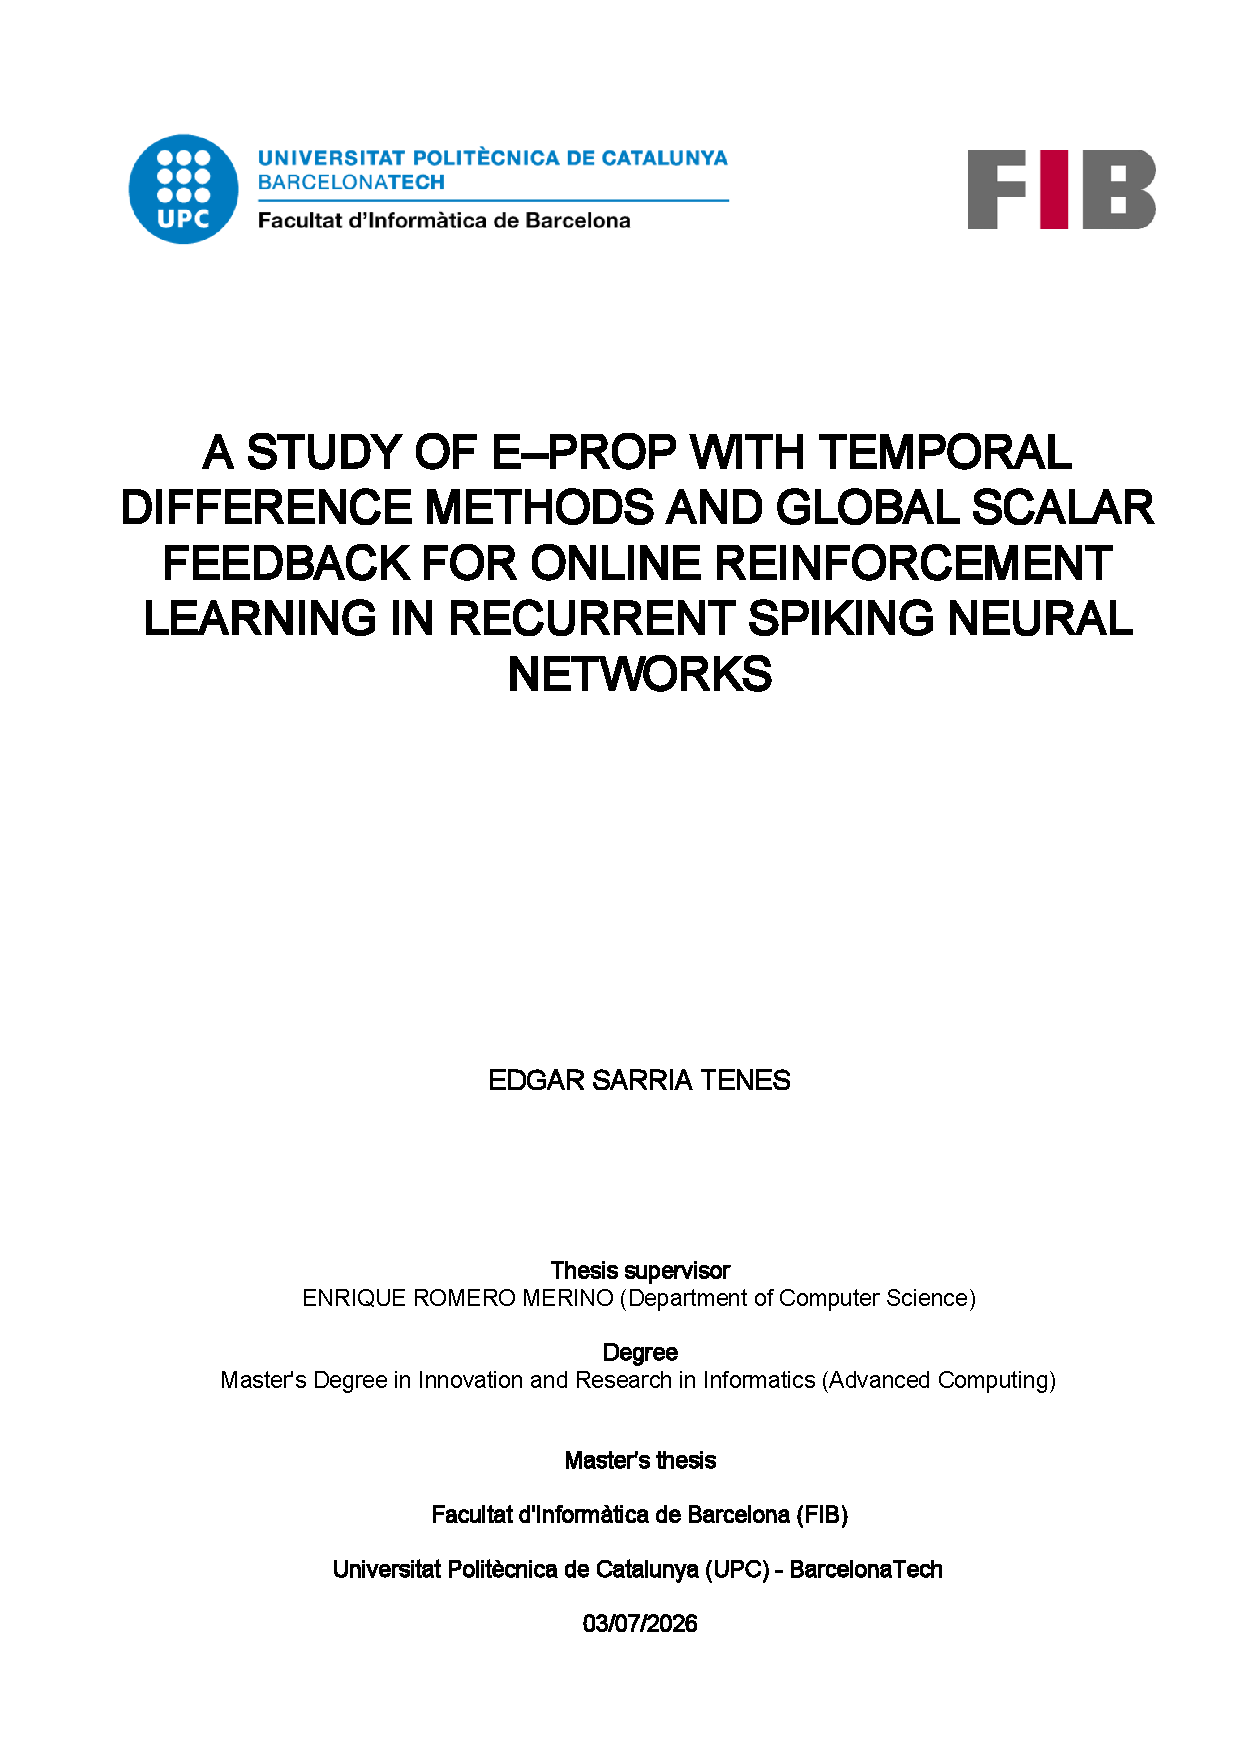
\includepdf[pages=-]{pdfs/portada_TFM.pdf}

% Abstract
\chapter*{Abstract}
\addcontentsline{toc}{chapter}{Abstract}

Training recurrent neural networks online, without storing past activity or
performing backward passes through time, remains an open problem,
particularly in reinforcement learning settings where feedback is delayed and 
sparse. This thesis studies this
problem in spiking recurrent neural networks (SRNNs) using e-prop
\citep{eprop2020}, a learning framework that decomposes the loss gradient
into locally computable eligibility traces and a neuron-specific learning
signal, avoiding the unbounded memory requirements of Backpropagation
Through Time and the prohibitive computational cost of Real-Time Recurrent
Learning.

The thesis makes two main contributions. The first is the implementation
of a continuously running reinforcement-learning agent based on an
excitatory-inhibitory SRNN, trained online using the e-prop
framework, without episodic resets, in a GPU-accelerated, event-based
simulation substrate. As part of this implementation, we integrate
$TD(\lambda)$ into the e-prop update rule, decoupling the discount factor
$\gamma$ from the credit-assignment decay $\lambda$. Stable value
estimation requires a small $\gamma$, while effective action-credit
assignment requires a longer horizon, and a single shared parameter cannot
satisfy both. This decoupling preserves long-range credit assignment
without destabilizing the critic.

The second contribution is \emph{distributed e-prop}, a new
learning algorithm that eliminates the structured feedback weights used by
standard e-prop to route loss information back to each neuron. Building on
the connection between perturbation-based learning and policy gradient
methods, every neuron is instead treated as an independent stochastic
actor that perturbs its own membrane dynamics and correlates this local
exploration with a single, identical, globally broadcast
temporal-difference error, relying entirely on its own local activity,
with no main policy gradient information required.

We evaluate this agent and learning rule on Snake, Pac-Man and Connect Four 
variants designed to probe reward credit assignment,
working memory, and behavioral adaptation under partial observability.
Across these tasks, distributed e-prop is found to be competitive with,
and in several settings more robust than, standard e-prop variants relying on  
adaptively learned feedback weights. The two
families of learning rules nonetheless differ systematically in their
sensitivity to architectural depth, $\lambda$,
and assumptions about neuron dynamics such as refractory-period
integration, indicating that local, perturbation-based credit assignment
and structured feedback-based credit assignment occupy different regions of the bias-variance tradeoff inherent to
online learning in SRNNs.

% Acknowledgments
\chapter*{Acknowledgments}
\addcontentsline{toc}{chapter}{Acknowledgments}

I would like to thank my supervisor for their guidance and support throughout this project. I am particularly grateful for providing the Pac-Man code used to run the experiments and produce the results presented in this work.
I also thank the developers and contributors of \texttt{ml\_genn} \cite{Yavuz2016GeNN} for making their open-source software and documentation available, which supported the implementation and evaluation of the experiments in this project.

\clearpage

\chapter*{Note on the Use of AI Assistance}

Parts of this thesis were produced with the assistance of large language models. These tools were used in three ways: as an
aid for understanding and exploring source material and related literature, as a
writing assistant for phrasing, restructuring, and improving the clarity of prose,
and as a coding aid in the development of parts of the experimental implementation.
All technical content, mathematical derivations, experimental design, results, and
conclusions are entirely the author's own work. The author takes full responsibility
for the accuracy and integrity of everything presented in this document.

% Table of contents
\tableofcontents
\listoffigures
\addcontentsline{toc}{chapter}{List of Figures}

\listoftables
\addcontentsline{toc}{chapter}{List of Tables}


\chapter{Introduction}
\label{ch:introduction}

\section{Context}
\label{sec:context}

A neural network is a computational model loosely inspired by the structure of the brain, a large collection of simple processing units, connected by weighted links, that together learn to perform complex tasks from experience. Most neural networks process their input in a single forward sweep, where each unit reads from the previous layer, computes an output, and passes it on. For many tasks, this is sufficient.

Some tasks, however, are inherently stateful. Understanding spoken language, controlling a robot in motion, or responding to a continuous stream of sensor readings all require the network to maintain some memory of what has happened and use it to interpret what is happening now. Networks designed for this purpose are called recurrent neural networks, and they differ from their simpler counterparts by feeding the output of the individual neurons to the other neurons in the network, thereby influencing future outputs. This creates a form of internal memory, but it also creates a training problem. When we want to adjust the network's parameters to improve its behavior, we need to account for the fact that a change made now may only affect the network's output many steps later. Tracing that delayed influence back to its cause requires unrolling the entire computation history, storing it in memory, and performing a separate backward pass through it once a full sequence has been processed.

This approach works well when sequences are short and data can be collected in batches. It is poorly suited, however, to settings where data arrives continuously, decisions must be made in real time, and no natural stopping point exists at which to pause and compute gradients. These settings (continuous control, online decision-making, real-time processing) are precisely the ones where neural networks might be most useful in practice, and yet they are where the standard training procedure is hardest to apply.

This thesis contributes to the problem of training recurrent networks in these continuous, real-time settings. It does so through the lens of spiking neural networks which are a class of recurrent network in which units communicate not through continuous numerical values but through discrete binary pulses, or spikes, much like neurons in the brain. These networks present additional challenges for training, but their temporal dynamics and sparse activity patterns make them a natural fit for the kinds of tasks considered here, and for the specialized hardware increasingly being developed to run them efficiently.

\section{Motivation}

A major long-term motivation behind biologically inspired learning research is the striking gap between artificial and biological learning systems. Biological organisms are capable of learning continuously from ongoing interaction with the environment, adapting to new situations in real time, operating under extremely limited energy budgets, and doing so without access to the large curated datasets, repeated training epochs, or explicitly defined objective functions commonly required in modern machine learning systems.

In contrast, many successful artificial learning methods rely heavily on offline optimization procedures, large-scale memory usage, and precisely structured gradient information. While these methods achieve remarkable performance in controlled settings, they remain comparatively inflexible, energy-intensive, and difficult to deploy in continuously adaptive environments.

Although biological neural systems are still only partially understood, their existence suggests that efficient online learning may be achievable using mechanisms fundamentally different from those employed by standard deep learning methods. This provides strong motivation for continuing to explore biologically inspired approaches to learning, not only as models of neural computation, but also as a potential source of new principles for scalable, adaptive, and energy-efficient artificial intelligence systems.

Many real-world learning problems do not come in the form of short, neatly separated sequences with clear beginnings and endings. A robot interacting with its environment, an autonomous system processing sensor streams, or an adaptive agent operating continuously in time must make decisions while new information keeps arriving. In these settings, learning cannot be treated as an offline procedure performed after the interaction has finished. The system must instead adapt continuously while it is operating, often under strict constraints on memory, latency, and energy consumption.

Recurrent neural networks are naturally suited to these problems because they can maintain internal state over time. Their dynamics allow past information to influence future behavior, enabling memory, temporal integration, and sequential decision-making. However, the standard methods used to train recurrent networks are poorly matched to the conditions under which these networks are most useful in practice.

The dominant approach for training recurrent systems, Backpropagation Through Time (BPTT), requires storing the full history of network activity and propagating gradients backward through it once a sequence has been processed. This works well in offline settings with finite sequences and batch processing, but becomes problematic in continuous environments where interaction may never stop and parameter updates are needed immediately. As sequences grow longer, memory usage increases, updates become delayed, and learning becomes increasingly difficult to perform online.

The problem becomes even more challenging in reinforcement learning. In this setting, the network is not provided with explicit target outputs, but instead learns from scalar rewards that may arrive long after the actions or internal computations that caused them. A successful learning rule must therefore solve the temporal credit assignment problem, defined as the problem of determining which past neural activities were responsible for the current activity. Solving this problem without storing complete histories is one of the central challenges of online learning in recurrent systems.

Eligibility traces provide a promising alternative. Instead of reconstructing the full history of the network during a backward pass, they maintain a running local memory of how recent neural activity has contributed to the neurons state. This makes them naturally compatible with online learning, since updates can be computed incrementally using only information available at the current timestep.

Spiking neural networks provide an especially interesting setting for studying these ideas. Because neurons communicate through sparse discrete spikes and integrate information over time through their internal dynamics, temporal processing is built directly into the architecture itself. Their event-driven operation also makes them attractive for neuromorphic hardware designed for low-power, real-time computation. However, training spiking networks remains difficult, particularly in reinforcement learning settings where feedback is delayed and learning must occur continuously.

Beyond their computational properties, spiking neural networks also offer a useful conceptual perspective inspired by biological learning. In biological neural systems, synaptic updates depend primarily on information locally available at each synapse, while evaluative signals such as dopamine are broadcast broadly across large populations of neurons. This suggests the possibility that effective learning may not require precise, structured error signals, but could instead emerge from the interaction between local activity traces and a shared globally broadcasted feedback signal.

This observation motivates the central question of this work: whether recurrent spiking neural networks can learn effectively in fully online reinforcement learning settings using learning rules that rely only on local computations and globally broadcast reward-based signals. More specifically, this thesis investigates whether such minimal and distributed learning mechanisms can remain competitive with more structured approaches while preserving scalability, locality, and online operation.

\section{Contributions}

This thesis makes two main contributions.

The first is the implementation of a continuously running, reinforcement-learning agent
based on spiking neural networks, trained online using the e-prop framework of \cite{eprop2020}. The agent operates without episodic resets, in a
GPU-accelerated event-based simulation environment, and is evaluated on tasks designed
to probe temporal credit assignment, working memory, and behavioral adaptation.

The second contribution is a new family of learning rules, which we refer to as distributed
e-prop, that build on the theoretical connection between
perturbation-based learning and policy gradient methods while borrowing the local structure of e-prop. Its central aim is to make
the learning rule as distributed as possible, rather than routing structured gradient
information back to individual neurons, every neuron receives the same single scalar
feedback signal and relies entirely on its own local activity to determine how its
incoming connections should be updated. Whether this minimal signal is sufficient for
effective learning, and under what conditions it becomes a limitation, is one of the central empirical questions this work aims to answer.

\chapter{Background and State of the Art}
\label{ch:sota}

This chapter establishes the theoretical foundations of this work and reviews
the relevant prior literature. We begin by introducing the core concepts and
notation used throughout the thesis, covering recurrent and spiking neural
networks, eligibility traces, and the reinforcement learning framework. We
then survey the state of the art in training recurrent networks online,
tracing the progression from classical backpropagation through time to eligibility-based and perturbation-based methods, and concluding with
the existing approaches to online reinforcement learning in spiking networks
that most directly motivate the contributions of this work.

% ============================================================
\section{Preliminaries and Notation}
\label{sec:preliminaries}

This section briefly introduces the core concepts and notation used
throughout this work. It is intended as a quick reference. Each topic is developed in greater depth in the
sections that follow.

\subsection{Models of Neural Computation}

We consider \emph{recurrent neural networks} (RNNs), networks that maintain
an internal hidden state $h_t \in \mathbb{R}^n$ updated at each timestep as
$h_t = f(h_{t-1}, x_t; \theta)$, allowing past inputs to influence future
outputs. A special case of particular interest here is \emph{spiking neural
networks} (SNNs), in which neurons communicate through discrete binary events
$z^t_j \in \{0, 1\}$ instead of the traditional rate-based networks approach of applying continuous activation functions. Each neuron
maintains a membrane potential $v^t_j$ that integrates incoming spikes over
time and resets upon crossing a firing threshold $v_{th}$. This
discontinuous spike generation mechanism prevents standard gradient-based
optimization from being applied directly; the techniques used to overcome
this limitation are discussed in the following sections.

\subsection{Temporal Credit Assignment}

A fundamental difficulty in training recurrent networks is that a parameter
change at time $t$ may only manifest in the loss $E$ many steps later,
creating complex temporal dependencies in $\frac{\mathrm{d}E}{\mathrm{d}\theta}$.
Determining which past activities were responsible for a present outcome is
known as the \emph{temporal credit assignment problem}, and it is the central
challenge addressed by every method reviewed in this chapter.
\emph{Eligibility traces} $e^t_{ji}$ are per-synapse variables that maintain
a local, forward-in-time record of how weight $W_{ji}$ has shaped recent
neural activity. They form the backbone of the online learning rules
developed throughout this work, and their key advantage is that they can be
computed incrementally without storing the full history of network states.

\subsection{Reinforcement Learning}

An agent interacts with an environment by following a policy
$\pi(a \mid s)$, collecting rewards $R_t$ with the goal of maximizing the
discounted return $G_t = \sum_{k \geq 0} \gamma^k R_{t+1+k}$. The
\emph{state-value function} $v_\pi(s) = \mathbb{E}_\pi[G_t \mid S_t = s]$
captures the expected return from each state and satisfies the Bellman
consistency condition
\begin{equation}
    v_\pi(s) = \mathbb{E}_\pi\!\left[R_{t+1} + \gamma\, v_\pi(S_{t+1})
    \mid S_t = s\right].
\end{equation}
The degree to which this condition is violated at any given step is measured
by the \emph{temporal-difference (TD) error},
\begin{equation}
    \delta_t = R_{t+1} + \gamma V_{t+1} - V_t,
\end{equation}
which serves as the primary online learning signal throughout this work.

\subsection{Notation Summary}

\begin{table}[h]
\centering
\begin{tabular}{ll}
\toprule
\textbf{Symbol} & \textbf{Meaning} \\
\midrule
$h_t$                        & Hidden state at time $t$ \\
$x_t$                        & Input at time $t$ \\
$z^t_j$                      & Spike output of neuron $j$ at time $t$ \\
$v^t_j$                      & Membrane potential of neuron $j$ at time $t$ \\
$v_{th}$                     & Spike threshold \\
$\alpha$                     & Membrane decay factor \\
$\mathcal{F}_\alpha$         & Exponential decay filter with parameter $\alpha$ \\
$W_{ji}$                     & Synaptic weight from neuron $i$ to $j$ \\
$e^t_{ji}$                   & Eligibility trace for synapse $ji$ at time $t$ \\
$L^t_j$                      & Learning signal for neuron $j$ at time $t$ \\
$E$                          & Loss function \\
$S_t,\ A_t,\ R_t$            & RL state, action, and reward at time $t$ \\
$\pi(a \mid s)$              & Stochastic policy \\
$G_t$                        & Discounted return at time $t$ \\
$\gamma$                     & Discount factor \\
$V_t$                        & Value estimate at time $t$ \\
$\delta_t$                   & Temporal-difference error \\
$\epsilon_j,\ \epsilon_{ji}$ & Perturbation at neuron $j$ or synapse $ji$ \\
\bottomrule
\end{tabular}
\caption{Summary of notation used throughout this work.}
\label{tab:notation}
\end{table}

% ============================================================
\section{Learning in Recurrent Neural Networks}
\label{sec:rnn-learning}

Having established the basic framework, we now turn to the problem of
training recurrent networks. This section describes the dominant approach,
Backpropagation Through Time, and explains why its structural requirements
make it poorly suited to the online, continuous-interaction settings that
motivate this work.

Recurrent Neural Networks (RNNs) have long been recognized as harder to
train than regular feedforward networks
\citep{learningLongTermHard, Werbos1990BackpropagationTT}. Recurrence
introduces temporal dynamics and dependencies into the network; past neural
activations influence current states, which significantly complicates the
process of gradient estimation. In feedforward networks, all causal
dependencies are separated by the topological ordering of the network.
This allows the backpropagation algorithm to accumulate gradient information
locally at each neuron by propagating errors backward through the network
layers. Although backpropagation is not online in time, it does not require
access to future network states beyond the current forward pass.

In recurrent networks, however, temporal dependencies prevent such a
separation. The effect of a neural activation at time $t$ may only become
apparent at much later times, meaning that full gradient computation requires
access to future network states.

\subsection{Backpropagation Through Time}

The canonical solution to the previously stated problem is Backpropagation Through Time (BPTT) \citep{Werbos1990BackpropagationTT}. The main idea is to convert the recurrent network into a feedforward network by unrolling it, making each timestep a "layer" of neurons that get their input from the previous state of the neurons, and influence the next "layer" in the next timestep. 

The unrolled network then could be understood as a flexible in size network with shared weights between all layers. BPTT is able to compute the exact gradient in RNNs, but, only if all network states through time have been stored. To "see" the effect of an activation of a neuron, the backpropagation algorithm needs to access the information in the future, where it can see the effect in the loss function and propagate backwards the loss information. 

We can see then, that to observe how the temporal dynamics of an RNN at the timestep $t$ influence the loss at $t+n$ we need to store all network states from $t$ to $t+n$, leading to memory requirements that scale linearly with the sequence length.

\subsection{Limitations for Online Learning}

Even though BPTT has been highly successful in practice, its need to store past activities and to perform backward passes over complete sequences prevents it from being a true online algorithm, especially in continuous data stream settings \citep{OSTL}. When dealing with very long or unbounded sequences, the history used by BPTT must be truncated, which introduces additional limitations. As discussed in \citet{OSTL}, citing earlier work by
\citet{WilliamsZipser1995} and \citet{Jaderberg2016}:

\begin{quote}
Truncated BPTT (TBPTT) reduces the amount of information that needs to be stored by splitting the input stream
into shorter segments and by updating the parameters of the
network after each segment (Williams and Zipser 1995).
However, it still leads to so-called system-locking problems (Jaderberg et al. 2016), because the parameter updates
can only be computed after the last input of each segment
has been processed. In addition, TBPTT encounters learning
deficiencies in tasks where there are long time lags between
the network activity and the feedback from the environment.
\end{quote}

These limitations make TBPTT poorly suited for strictly online learning scenarios and tasks with long temporal dependencies.

\section{Online Learning in Recurrent Systems}

\subsection{Requirements for Online Learning}

We understand online learning as a learning paradigm in which model
parameters are updated incrementally as data is processed, without
requiring access to future inputs or the storage of complete past
trajectories \citep{eprop2020, UORO}. In recurrent systems, this implies that learning updates should be computed at each timestep using information locally available at that time, making online learning particularly suitable for continuous and potentially unbounded data streams.

This definition is intentionally strict with respect to which learning algorithms it includes. For instance, Backpropagation Through Time and its truncated variants rely on storing past network states over a temporal window and performing backward passes to apply the chain rule, which prevents parameter updates from being computed strictly at the current timestep. As a result, such methods do not satisfy the requirements of online learning as defined here.

Part of the motivation for adopting this definition is to move toward learning mechanisms that more closely resemble those observed in biological systems, while also benefiting from properties such as constant memory usage over time, low-latency updates, and suitability for continuous, non-episodic interaction with dynamic environments. 

\subsection{Real-Time Recurrent Learning}

Real-Time Recurrent Learning (RTRL), introduced by \citet{RTRL}, provides a principled solution to the online learning problem in recurrent neural networks by computing exact gradients in a purely forward-in-time manner. In contrast to Backpropagation Through Time, RTRL does not require storage of past activations or a backward pass through time. Instead, it incrementally maintains derivatives of the hidden state with respect to the network parameters as the sequence unfolds.

Consider a recurrent neural network with hidden state $h_t$ and parameters $\theta$. RTRL maintains, at each time step $t$, the quantity:
\[
\frac{\partial h_t}{\partial \theta},
\]
which represents how changes in the parameters influence the current hidden state. This quantity is updated recursively using the chain rule as new inputs arrive. If we denote the recurrent update as $h_t = f(h_{t-1}, x_t; \theta)$, then the derivative evolves according to:
\[
\frac{\partial h_t}{\partial \theta}
=
\frac{\partial f}{\partial h_{t-1}} \frac{\partial h_{t-1}}{\partial \theta}
+
\frac{\partial f}{\partial \theta}.
\]

This recursion ensures that the influence of all past parameter changes is continuously propagated forward in time, enabling exact gradient computation at each timestep without revisiting past states.

However, the main limitation of RTRL lies in its computational cost. For a network with $n$ hidden units, the Jacobian $\frac{\partial h_t}{\partial \theta}$ is a three-dimensional tensor, leading to a naive computational complexity of $O(n^4)$ per timestep and memory complexity of $O(n^3)$. This arises from the need to track how every parameter affects every hidden unit through time, and how these effects interact multiplicatively through recurrent connections.

In practice, this cost makes standard RTRL infeasible for networks of realistic size. As a result, much of the modern literature focuses on approximations that reduce this complexity while preserving the online nature of the algorithm. Examples include Unbiased Online Recurrent Optimization (UORO) \citep{UORO}, which reduces the rank of the Jacobian estimate, and more recent structured approximations such as Kronecker-Factored RTRL (KF-RTRL), which exploit low-rank structure in the recurrent dynamics \citep{eprop2020}.

Despite its computational limitations, RTRL remains theoretically important as it represents the gold standard for online gradient computation in recurrent systems and provides the foundation for many biologically plausible and memory-efficient approximations. In particular, it highlights the key idea that learning in recurrent networks can be decomposed into (i) local eligibility traces capturing temporal credit assignment and (ii) learning signals that modulate these traces, a perspective that is further developed in modern approaches such as e-prop.

\section{Gradient Estimation with E-prop}
\label{sec:e-prop}
E-prop (eligibility propagation  \cite{eprop2020}) provides a framework for online learning in recurrent neural networks that addresses the limitations of both BPTT and RTRL. Instead of attempting to compute exact gradients through time or maintaining full Jacobians of the network dynamics, e-prop leverages a structural decomposition of the gradient into components that can be computed locally and components that carry information about the loss.

This perspective leads to learning rules in which synaptic updates are expressed as the interaction between locally computable eligibility traces and neuron-specific learning signals. The resulting algorithm operates in a strictly forward-in-time manner, requires constant memory with respect to sequence length, and remains applicable to networks with complex temporal dynamics.

In this section, we introduce e-prop in the context of spiking recurrent neural networks, where its interpretation in terms of local synaptic variables and global modulatory signals becomes particularly natural. We then derive the decomposition underlying e-prop and discuss practical variants that enable efficient and scalable learning.

\subsection{Spiking Recurrent Neural Networks}

Inspiration in biological systems has proven to be a good heuristic for system design. In this case, spiking recurrent neural networks (SRNNs) try to mimic the observed dynamics of the brain, where neurons communicate with pulses. Time is an intrinsic part of their design, even without recurrent connections the way they integrate past activations of connected networks enable them to remember information from many time steps ago. Recurrent connections then let the network not only remember the previous activations but "act" on them through time. It is clear then that the main tasks that these networks try to solve are time-related tasks, which involve temporal credit assignment.

The derivation in \cite{eprop2020} is made with SRNNs in mind, so it is important for us to understand how they define them and the additional problems they present. To quote \cite{eprop2020}:
\begin{quote}
We consider the arguably most prominent model for spiking neurons in the brain, the leaky integrate-and-fire (LIF) neurons, where spikes that arrive from other neurons through synaptic connections are multiplied with the corresponding synaptic weight, and are linearly integrated by a leaky membrane potential. The neuron fires—i.e., emits a spike—when the membrane potential reaches a firing threshold....Spikes are modeled as binary variables  $z^t_j$ that assume value $1$ if neuron $j$ fires at time $t$, otherwise value $0$. It is common in models to let $t$ vary over small discrete time steps, e.g., of $1\ ms$ length.  
\end{quote}
The dynamics of LIF neurons are defined by the equations
\begin{equation}
v^{t+1}_j = \alpha v^t_j + \sum_{i \neq j} W^{rec}_{ji} z^t_i + \sum_i W^{in}_{ji} x^{t+1}_i - z^t_jv_{th}
\end{equation}
\begin{equation}
z^t_j=H(v^t_j-v_{th})
\end{equation}
which can be interpreted as a leaky integration process where the membrane potential
retains a fraction $\alpha v^t_j$ of its previous value, accumulates incoming spikes
through the recurrent and input weights, and is reset by $v_{th}$ whenever the neuron emits a spike.

In addition, a refractory period is imposed by fixing $z^t_j = 0$ for a short interval after each spike. This constraint can be interpreted as a simple mechanism to regularize the neuron dynamics preventing arbitrarily high firing frequencies. As a result, the network is encouraged to represent information in its temporal structure, which improves stability significantly. 

Quoting \cite{eprop2020} again:
\begin{quote}
    $W^{rec}_{ji}$ ($W^{in}_{ji}$) is the synaptic weight from network (input) neuron $i$ to neuron $j$. The decay factor $\alpha$ in (6) is given by $e^{-\delta t/\tau_m}$ , where $\tau m$ (typically 20 ms) is the membrane time constant. $\delta t$ denotes the discrete time step size, which is set to $1 ms$ in our simulations. H denotes the Heaviside step function....the neurons membrane potential is reduced by a constant value after an output spike, which relates our model to the spike response $model^{53}$. To introduce a simple model of neuronal refractoriness, we further assume that $z^t_j$ is fixed to $0$ after each spike of neuron $j$ for a short refractory period of $2–5 ms$ depending on the simulation.
\end{quote}

To enhance the network capabilities we can also let the activation threshold update over time at a slower time scale than the integration dynamics, this type of neuron is called adaptive leaky integrate-and-fire (ALIF). These neurons have a two dimensional internal state $h^t_j \defeq \left[ v^t_j, a^t_j\right]$. Their threshold potential $A^t_j$ behaves in the following way:
\begin{equation}
A^t_j = v_{th} + \beta a^t_j
\end{equation}
\begin{equation}
a^{t+1}_j=\rho a^t_j + z^t_j
\end{equation}
Then the spikes take into account the threshold potential:
\begin{equation}
z^t_j=H(v^t_j-A^t_j)
\end{equation}
These network dynamics are not differentiable due to the discontinuous spike generation function. In particular, the derivative of $z^t_j = H(v^t_j - A^t_j)$ with respect to the membrane potential $v^t_j$ is zero almost everywhere and undefined at the threshold. As a result, standard gradient-based optimization cannot be applied directly.


To address this issue, surrogate gradient methods replace this non-existent
derivative with a smooth approximation \citep{Neftci2019Surrogate}. Concretely, a pseudo-derivative $\psi^t_j \approx \frac{\partial z^t_j}{\partial v^t_j}$ is introduced, which provides a non-zero gradient in a small region around the firing threshold. The pseudo-derivative used in \cite{eprop2020} is defined as:
\begin{equation}
\psi^t_j = \frac{1}{v_{th}}\gamma_{pd}\max \left( 0, 1- \left|\frac{v^t_j - A^t_j}{v_{th}} \right|\right)\ ;\ \text{where } \gamma_{pd}=0.3
\end{equation}
This function is non-zero only when the membrane potential $v^t_j$ is close to the threshold $A^t_j$, and vanishes otherwise. Intuitively, this means that gradients are propagated only when the neuron is close to firing, assigning credit to inputs that influenced the spike, or prevented it from happening.

During the refractory period, $\psi^t_j$ is set to $0$, since the neuron is prevented from firing and its dynamics are externally constrained. This ensures that no gradient is propagated during this interval, maintaining consistency between the forward dynamics and the learning rule.

\begin{figure}[h]
    \centering
    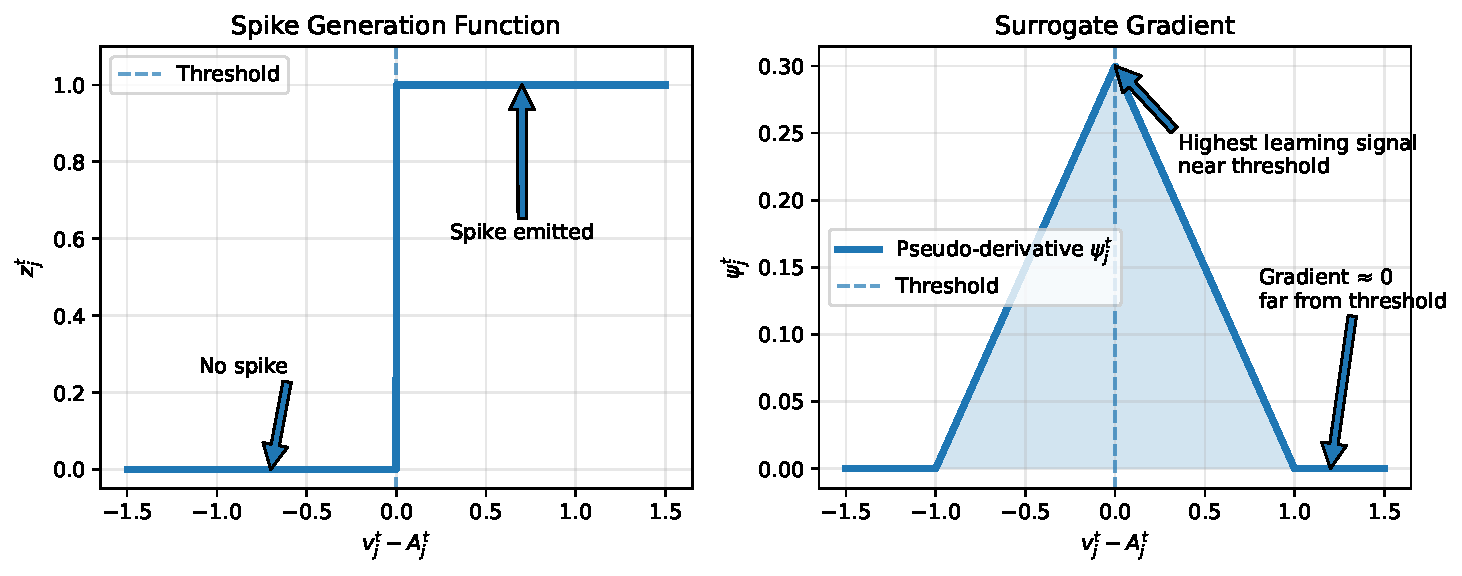
\includegraphics[width=1.0\linewidth]{images/spiking_function_dynamics.pdf}
    \caption[Spike generation and surrogate gradient]{Spiking function dynamics and surrogate gradient. Left: spike generation in a leaky integrate-and-fire neuron, modeled by the Heaviside function. A spike is emitted when the membrane potential exceeds the firing threshold. Right: pseudo-derivative used during learning. Because the true derivative of the Heaviside Step function is zero almost everywhere and undefined at threshold, it is replaced by a triangular surrogate gradient. The surrogate assigns the largest learning signal to membrane potentials close to threshold, where small input changes can alter the spiking decision, while activity far from threshold receives negligible credit.}
    \label{fig:spiking-function-dynamics}
\end{figure}

\clearpage
\subsection{E-prop: Separation of Local gradient and Loss gradient}

The key innovation of \cite{eprop2020} is the proof that the gradient $\frac{\mathrm{d}E}{\mathrm{d} W_{ji}}$ can be represented as a decomposition of two parts:
\begin{equation} \label{eq:epropDecomposition}
\sum_t \frac{\mathrm{d}E}{\mathrm{d}z^t_j} \cdot \left[ \frac{\mathrm{d}z_j^t}{\mathrm{d}{W_{ji}}} \right]_{local} 
\end{equation}

Quoting \cite{eprop2020}:
\begin{quote}
This local gradient is defined as a sum of products of partial
derivatives concerning the hidden state $h^t_j$ of neuron $j$ at time $t$ and preceding time steps, which can be updated during the
forward computation of the RNN by a simple recursion (Eq.(14)). This term $\left[ \frac{\mathrm{d}z_j^t}{\mathrm{d}{W_{ji}}} \right]_{local}$ is not an approximation. Rather, it collects the maximal amount of information about the network gradient $\frac{\mathrm{d}E}{\mathrm{d} W_{ji}}$ that can be computed locally in a forward manner. Therefore, it is the key-factor of e-prop. As it reduces for simple neuron models—whose internal state is fully captured by its membrane potential—to a variation of terms that are commonly referred to as eligibility traces
\end{quote}
They define the eligibility traces of the weight connecting the pre-synaptic neuron $i$ and the post-synaptic neuron $j$ ($e^t_{ji}$), and the loss signal for the output neuron $j$ ($L^t_j$) as:
$$
    e^t_{ji} \defeq \left[ \frac{\mathrm{d}z_j^t}{\mathrm{d}{W_{ji}}} \right]_{local}
    L^t_j \defeq \frac{\mathrm{d}E}{\mathrm{d}z^t_j} 
$$

The term $e^t_{ji}$ is referred to as the \emph{eligibility trace} because it captures the causal effect of the synapse from neuron $i$ to neuron $j$ on the firing of neuron $j$ at time $t$. In contrast, $L^t_j$ acts as a \emph{learning signal}, indicating the causal effect of the spike of neuron $j$ at time $t$ on the loss. This definition yields the following representation for the weights gradient:
\begin{equation} \label{eq:SumLossEtraces}
\frac{\mathrm{d}E}{\mathrm{d}W_{ji}} = \sum_t L^t_je^t_{ji}
\end{equation}

Having the weights' gradient, it is clear how to define an update rule that will minimize $E$ in an online manner, we have to update the weights at time $t$ proportional to $-L^t_je^t_{ji}$. If we use this definition by itself, we could not compute the actual weights gradient online; that is because $L^t_j$ is influenced by the spikes from previous time steps through recurrent connections in the network. To relax this requirement, $L^t_j$ is replaced by the partial derivative $\frac{\partial E}{\partial z^t_j}$, which only takes into account the direct influence of the spikes $z^t_j$.

\begin{figure}[h]\label{fig:EpropComputationFlow}
    \centering
    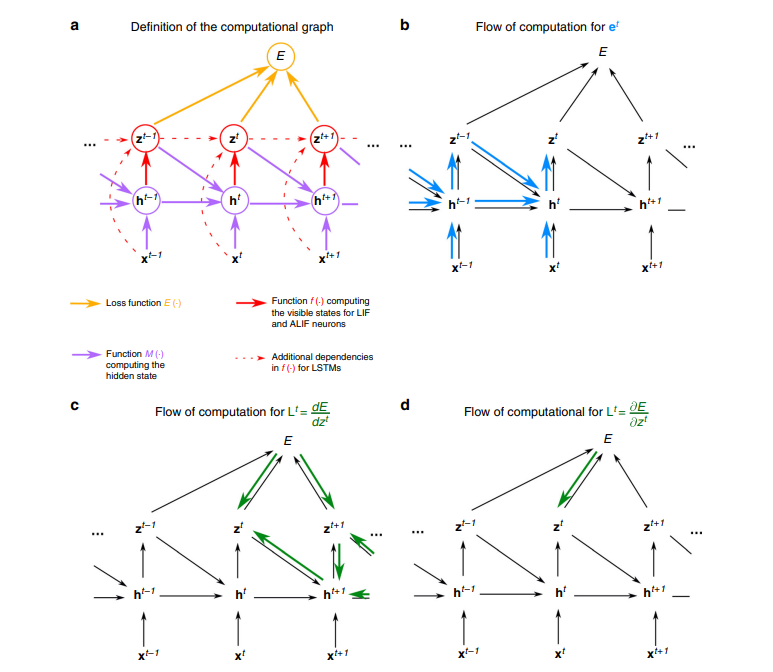
\includegraphics[width=1.0\linewidth]{images/EpropComputationFlow.png}
    \caption[E-prop computational graph (Bellec et al., 2020)]{%
    \textbf{Original caption from \citet{eprop2020}:} ``\textbf{Fig. 6 Computational graph and gradient propagations}. $\textbf{a}$ Assumed mathematical dependencies between hidden neuron states $\textbf{h}^t_j$ , neuron outputs $\textbf{z}^t$, network inputs $\textbf{x}^t$, and the loss function $E$ through the mathematical functions $E( \cdot ), M( \cdot ), f( \cdot )$ are represented by colored arrows. \textbf{b–d} The flow of computation for the two components $\textbf{e}^t$ and $\textbf{L}^t$ that merge into the loss gradients of Eq. (3) can be represented in similar graphs. \textbf{b} Following Eq. (14), the flow of the computation of the eligibility traces $e^t_{ji}$ is going forward in time. \textbf{c} Instead, the ideal learning signals $L^t_j = \frac{\mathrm{d}E}{\mathrm{d}z^t_j}$  requires to propagate gradients backward in time. \textbf{d} Hence, while $e^t_{ji}$ is computed exactly, $L^t_{j}$ is approximated in e-prop applications to yield an online learning algorithm.``}
    \label{fig:EpropComputationFlow}
\end{figure}
Figure \ref{fig:EpropComputationFlow} shows a diagram of the computation flow of the eligibility traces and the loss feedback; it can be clearly seen how the simplified version of $L^t$ does not use future interactions. The drawback of ignoring indirect effects is the introduction of bias from the true loss gradient, but it is necessary for the algorithm to work online.
\clearpage
\subsection{Symmetric, Random and Adaptive E-prop}
\label{subsec:eprop-variants}

To route the loss signals $L^t$ to the neurons in the network they define $B_{kj}$, which is the weight connecting neuron $j$ to output neuron $k$. At first glance, it seems natural to set $B_{kj} = W_{kj}$, giving symmetric e-prop. While this would compute the exact gradient in the absence of recurrent connections, it fails for neurons not connected directly to the output, which would receive no feedback.


Random e-prop solves this by assigning $B_{kj}$ random fixed values. It is quite unintuitive, but it is inspired in biological systems and it has been shown to work for feedback alignment networks (\cite{Lillicrap2016}). Feedback alignment networks use fixed random weights to propagate error signals. The idea of feedback alignment networks is that they adapt to the random projection of the losses, and the output weights undo the projection and make use of the random learning from the network. This gives us random e-prop. This way all neurons, even if they are not connected to the output, get feedback. This approach results in surprising performance, but has been shown that feedback alignment networks fail to train for deep image classification networks (\cite{eprop2020}). It is theorized that random e-prop would fail in a similar way.

Adaptive e-prop combines the benefits of symmetry and flexibility by initializing $B_{kj}$ to random values, and then updating with a learning rule similar to $W_{kj}$, gradually aligning feedback with the true gradient while maintaining online learning.

\section{Perturbation-Based Gradient Estimation}
\label{sec:perturbation}

Perturbation-based learning methods provide an alternative to gradient
backpropagation by estimating gradients through stochastic variations of
neural activity or synaptic weights. These methods are particularly appealing
in settings where exact gradient computation is not feasible, such as in
recurrent systems with long temporal dependencies, non-differentiable
dynamics, or biologically constrained learning mechanisms.

In contrast to Backpropagation Through Time (BPTT) and Real-Time Recurrent
Learning (RTRL), perturbation-based approaches do not require backward passes
through time or the storage of past network states. Instead, they rely on
correlations between stochastic perturbations and changes in a global
objective signal, such as a loss or reward.

\subsection{Weight Perturbation}

Weight perturbation is one of the earliest approaches to gradient estimation
in neural networks. The core idea is to apply small random perturbations
$\epsilon_{ij}$ to the synaptic weights and observe the resulting change in
the loss function. By the definition of the derivative, for small
perturbations:

\begin{equation}
E(W + \epsilon) - E(W) \approx \sum_{ij} \frac{\partial E}{\partial W_{ij}} \epsilon_{ij}
\end{equation}
Multiplying both sides by $\epsilon_{ij}$ and taking the expectation over
the perturbations, under the assumption that $\epsilon_{ij}$ are independent
with zero mean and variance $\sigma^2$:

\begin{equation}
\mathbb{E}\left[ \frac{(E(W+\epsilon) - E(W)) \, \epsilon_{ij}}{\sigma^2} \right] = \frac{\partial E}{\partial W_{ij}}
\end{equation}
This gives an unbiased estimator of the gradient that requires only two
forward passes and no backpropagation. However, it suffers from high
variance, since the perturbation of every other weight contributes noise to
the estimate of each individual gradient. The variance therefore grows with
the number of parameters, making this approach inefficient for large
networks.
\subsection{Node Perturbation}

Node perturbation reduces this variance by injecting noise into neuronal
activities. Let $\epsilon_j^t$ denote
a stochastic perturbation applied to the activity of neuron $j$ at time $t$.
The gradient of the loss with respect to weight $W_{ij}$ can be decomposed
using the chain rule as:

\begin{equation}
\frac{\partial E}{\partial W_{ij}} = \frac{\partial E}{\partial z_j^t} \cdot
\frac{\partial z_j^t}{\partial W_{ij}}
\end{equation}
The perturbation $\epsilon_j^t$ provides a stochastic estimate of
$\frac{\partial E}{\partial z_j^t}$ through the observed change in loss,
while $\frac{\partial z_j^t}{\partial W_{ij}}$ is approximated by the
presynaptic activity $z_i^t$, which is the exact derivative of the neuron's
linear input with respect to $W_{ij}$. This gives the gradient estimate:

\begin{equation}
\Delta W_{ij} \propto -(E - \bar{E}) \cdot \epsilon_j^t \cdot z_i^t
\end{equation}
where $\bar{E}$ is a baseline used to reduce variance. The key advantage
over weight perturbation is that the perturbation space now has
dimensionality equal to the number of neurons instead of the number of
weights, which is typically much smaller, leading to lower variance gradient
estimates.

However, node perturbation introduces a different kind of imprecision, a
single perturbation $\epsilon_j^t$ affects all synapses onto neuron $j$
simultaneously, so the gradient estimate for each individual weight $W_{ij}$
gets shared credit over all weights, losing causal resolution.

\subsection{Limitations and Challenges}

Despite their conceptual simplicity and biological plausibility,
perturbation-based methods suffer from a fundamental variance problem.
Gradient information is inferred indirectly from correlations between
stochastic perturbations and changes in a global loss or reward signal,
which produces noisy estimates. In weight perturbation, the variance grows
rapidly with the number of parameters because the effect of every
perturbation contributes to the observed loss change. Node perturbation
reduces this variance by operating in a lower-dimensional perturbation
space, but at the cost of coarser credit assignment, since all synapses
onto a neuron share the same perturbation signal.

In recurrent and temporally extended systems, perturbation-based methods
can in principle assign credit across long time intervals without
backpropagation through time. However, the influence of a perturbation may
only become apparent much later through its effect on the final loss or
reward, making the relevant correlations difficult to estimate reliably.
As a result, learning often becomes increasingly sample-inefficient as the
temporal horizon grows.

These limitations motivate approaches that augment perturbation-based
estimators with additional structure, such as eligibility traces, which
preserve local information about past activity and improve temporal credit
assignment. Such methods will be discussed in Chapter~\ref{ch:method}.

\section{Online Reinforcement Learning}
\label{sec:online-rl}
 Reinforcement learning addresses the problem of learning to act through interaction with an environment in order to maximize cumulative reward. In contrast to supervised learning, where explicit targets are provided, RL relies on scalar reward signals that may be delayed and only indirectly related to the actions that caused them.

We follow the formal framework presented in \citet{SuttonBarto2018}, where the interaction between agent and environment is modeled as a Markov Decision Process (MDP). At each discrete time step $t$, the agent observes a state $S_t$, selects an action $A_t$ according to a policy $\pi$, receives a reward $R_{t+1}$, and transitions to a new state $S_{t+1}$. The goal is to maximize the expected return $G_t$.

\subsection{Weighting the Reward Temporal Credit Horizon with TD($\lambda$)}

Temporal-Difference (TD) learning provides a mechanism for learning the
value function in an online manner. Recall from the Bellman equation that
the value function satisfies:
\begin{equation}
    v_\pi(s) = \mathbb{E}_\pi \left[ R_{t+1} + \gamma v_\pi(S_{t+1}) \mid S_t = s \right]
\end{equation}
This equation says that the value of a state must equal the expected
immediate reward plus the discounted value of the next state. If our current
estimate $V(S_t)$ were perfect, this consistency condition would hold
exactly. The TD error measures how far we are from satisfying it:
\begin{equation}
\delta_t = R_{t+1} + \gamma V(S_{t+1}) - V(S_t),
\end{equation}
which is zero when $V(S_t) = R_{t+1} + \gamma V(S_{t+1})$, that is
when the Bellman equation is satisfied. The TD error therefore provides a
natural online signal for updating $V$ toward consistency, and the update
rule for a parameterized value function $V(S_t; \boldsymbol{\theta})$ is:
\begin{equation}
\boldsymbol{\theta}_{t+1} = \boldsymbol{\theta}_t + \alpha \, \delta_t \, \nabla_{\boldsymbol{\theta}}
V(S_t; \boldsymbol{\theta}_t)
\end{equation}
where $\alpha$ is the learning rate. Importantly, this update can be
performed online at each time step using only currently available
information, making TD methods well aligned with the requirements for online
learning described earlier.

\paragraph{Forward view.}
One-step TD uses only the immediate next reward and value estimate to update
$\boldsymbol{\theta}$, which is computationally cheap but ignores information from
further into the future. A natural generalization is to look further ahead
and define the $n$-step return:
\begin{equation}
    G_t^{(n)} = \sum_{k=0}^{n-1} \gamma^k R_{t+1+k} + \gamma^n V(S_{t+n})
\end{equation}
which uses the next $n$ actual rewards before bootstrapping with the value
estimate. As $n \to \infty$, this recovers the full Monte Carlo return $G_t$.
TD$(\lambda)$ takes a weighted average of all $n$-step returns:
\begin{equation}
\label{eq:advantage-sum}
    G_t^\lambda = (1-\lambda) \sum_{n=1}^{\infty} \lambda^{n-1} G_t^{(n)}
\end{equation}
where $\lambda \in [0,1]$ controls how far into the future the returns are
accumulated. Setting $\lambda = 0$ recovers the one-step TD update, while
$\lambda = 1$ recovers the full Monte Carlo return. This forward view makes
the correctness of TD$(\lambda)$ transparent, we can see that it is the weighted
average of consistent return estimates.

A useful property that connects the forward view to the TD error is that
the discounted sum of TD errors over a trajectory recovers the advantage
exactly:
\begin{equation} \label{eq:td_return_identity}
    G_t - V_t = \sum_{t' \geq t} \gamma^{t'-t} \delta_{t'},
\end{equation}
when using the true value function. This identity shows that accumulating
TD errors forward in time is equivalent to computing how much better the
actual return was compared to the current value estimate, and justifies
using the running sum of $\delta_t$ as an online surrogate for the full
return. Setting $\lambda = 1$ in the backward view recovers this full
accumulation, while $\lambda = 0$ uses only the immediate TD error.

\paragraph{Backward view.}
While the forward view makes correctness clear, it requires storing future
returns, which is incompatible with online learning. The backward view
provides an equivalent formulation that can be computed incrementally. The
key insight is that, we can
maintain a decaying memory of past gradients called an \emph{eligibility
trace}:
\begin{equation}
e_t = \gamma \lambda e_{t-1} + \nabla_{\boldsymbol{\theta}} V(S_t; \boldsymbol{\theta}_t)
\end{equation}
and update the parameters at each timestep as:
\begin{equation}
\boldsymbol{\theta}_{t+1} = \boldsymbol{\theta}_t + \alpha \, \delta_t \, e_t
\end{equation}
The eligibility trace $e_t$ accumulates a decaying history of past gradients,
assigning more weight to recent states. When a TD error $\delta_t$ arrives,
it is applied not just to the current gradient but to all past gradients
weighted by how recently they occurred. It can be shown that this backward
view produces exactly the same expected update as the forward view
\citep{SuttonBarto2018}, while being fully online and requiring only constant
memory. Intermediate values of $\lambda$ trade off variance from long
accumulations against bias from short ones, and the eligibility trace
provides a natural mechanism for temporal credit assignment that is
conceptually closely related to the eligibility traces introduced in e-prop.


\subsection{Policy Gradient Methods}
\label{sec:policygradient}
While value-based methods aim to estimate value functions, policy gradient
methods directly optimize a parameterized policy $\pi(a \mid s; \boldsymbol{\theta})$ by
ascending the gradient of the expected return with respect to the policy
parameters $\boldsymbol{\theta}$ \citep{Williams1992REINFORCE}.

\paragraph{What we want to compute.}
The objective is to maximize the expected return $J(\boldsymbol{\theta})$,
defined as the expected cumulative reward under trajectories generated by the
policy:
\begin{equation}
    J(\boldsymbol{\theta}) = \mathbb{E}_{p_{\boldsymbol{\theta}}} \left[ G(\tau) \right],
\end{equation}
where $\tau = (S_0, A_0, R_1, S_1, A_1, \ldots)$ denotes a full trajectory,
and $G(\tau)$ is its discounted return. To maximize $J(\boldsymbol{\theta})$
by gradient ascent, we need to compute $\nabla_{\boldsymbol{\theta}}
J(\boldsymbol{\theta})$.

\paragraph{Writing the expectation as an integral.}
By definition, the expectation over trajectories is an integral weighted by
the trajectory probability $p_{\boldsymbol{\theta}}(\tau)$:
\begin{equation}
    J(\boldsymbol{\theta})
    = \int p_{\boldsymbol{\theta}}(\tau) \, G(\tau) \, \mathrm{d}\tau
\end{equation}
To compute the gradient, we move $\nabla_{\boldsymbol{\theta}}$
inside the integral. Under standard regularity conditions (smooth dependence
on $\boldsymbol{\theta}$ and fixed support), this yields:
\begin{equation}
    \nabla_{\boldsymbol{\theta}} J(\boldsymbol{\theta})
    = \int \nabla_{\boldsymbol{\theta}} p_{\boldsymbol{\theta}}(\tau)
    \, G(\tau) \, \mathrm{d}\tau
\end{equation}

\paragraph{The log-derivative trick.}
The expression above is not yet an expectation under $p_{\boldsymbol{\theta}}$,
since the $p_{\boldsymbol{\theta}}(\tau)$ weighting the integral has been
consumed by the gradient. To recover the expectation form, we apply the
log-derivative identity:
\begin{equation}
    \nabla_{\boldsymbol{\theta}} p_{\boldsymbol{\theta}}(\tau)
    = p_{\boldsymbol{\theta}}(\tau) \,
    \nabla_{\boldsymbol{\theta}} \log p_{\boldsymbol{\theta}}(\tau),
\end{equation}
which follows from the chain rule. Substituting this into the integral and
recognising the definition of expectation gives:
\begin{equation}
    \nabla_{\boldsymbol{\theta}} J(\boldsymbol{\theta})
    = \int p_{\boldsymbol{\theta}}(\tau) \,
    \nabla_{\boldsymbol{\theta}} \log p_{\boldsymbol{\theta}}(\tau) \,
    G(\tau) \, \mathrm{d}\tau
    = \mathbb{E}_{p_{\boldsymbol{\theta}}} \left[
        G(\tau) \, \nabla_{\boldsymbol{\theta}} \log p_{\boldsymbol{\theta}}(\tau)
    \right]
\end{equation}
This is useful because expectations can be estimated by sampling as we can run
the policy in the environment, collect trajectories, and average
$G(\tau) \, \nabla_{\boldsymbol{\theta}} \log p_{\boldsymbol{\theta}}(\tau)$
over those samples.

\paragraph{Policy-dependent terms.}
The probability of a trajectory factorizes over time steps as:
\begin{equation}
    p_{\boldsymbol{\theta}}(\tau)
    = p(S_0) \prod_{t} \pi(A_t \mid S_t; \boldsymbol{\theta})
    \, P(S_{t+1} \mid S_t, A_t)
\end{equation}
Taking the logarithm turns the product into a sum:
\begin{equation}
    \log p_{\boldsymbol{\theta}}(\tau)
    = \log p(S_0)
    + \sum_t \log \pi(A_t \mid S_t; \boldsymbol{\theta})
    + \sum_t \log P(S_{t+1} \mid S_t, A_t)
\end{equation}
We now make the standard reinforcement learning assumption that the
environment dynamics $P(S_{t+1} \mid S_t, A_t)$ do not depend on the policy
parameters $\boldsymbol{\theta}$. Under this assumption, only the policy
terms contribute to the gradient, yielding:
\begin{equation}
    \nabla_{\boldsymbol{\theta}} \log p_{\boldsymbol{\theta}}(\tau)
    = \sum_t \nabla_{\boldsymbol{\theta}} \log \pi(A_t \mid S_t;
    \boldsymbol{\theta})
\end{equation}
Substituting back gives the Policy Gradient Theorem:
\begin{equation}
\nabla_{\boldsymbol{\theta}} J(\boldsymbol{\theta})
= \mathbb{E}_{p_{\boldsymbol{\theta}}} \left[ G(\tau) \sum_t
\nabla_{\boldsymbol{\theta}} \log \pi(A_t \mid S_t; \boldsymbol{\theta}) \right]
\end{equation}
The intuition behind $\log \pi$ can be understood by examining the form of the gradient. The term $\nabla_{\boldsymbol{\theta}} \log \pi(A_t \mid S_t; \boldsymbol{\theta})$ measures how the log-probability of the selected action changes with respect to the parameters. When multiplied by the return $G(\tau)$, it leads to an update that increases the probability of actions that resulted in high returns, and decreases the probability of those that led to 
poor outcomes.

Importantly, the magnitude of this update depends on how probable the action was under the current policy. Since the gradient of the log-probability scales inversely with probability, actions that were unlikely under the policy but led to high returns produce larger updates. In other words, surprising successful actions are reinforced more strongly than already likely ones. If an action with low prior probability turns out to be beneficial, the policy adapts rapidly to increase its likelihood. Conversely, highly probable actions that yield low returns are suppressed. This balance between reinforcing successful behavior and correcting overconfident decisions is at the core of policy gradient methods.

\subsection{Actor-Critic Methods}

The policy gradient derived above uses the return $G(\tau)$ to weight the updates. While this estimator is unbiased, it typically exhibits high variance, which can make learning unstable. A standard technique to reduce this variance is to introduce a baseline $b(S_t)$ that does not depend on the action:
\begin{equation}
\nabla_{\boldsymbol{\theta}} J(\boldsymbol{\theta})
= \mathbb{E}_{p_{\boldsymbol{\theta}}} \left[
\sum_t \left( G_t - b(S_t) \right)
\nabla_{\boldsymbol{\theta}} \log \pi(A_t \mid S_t; \boldsymbol{\theta})
\right].
\end{equation}
Subtracting such a baseline does not change the expected value of the gradient, since:
\begin{equation}
\mathbb{E}_{\pi} \left[
b(S_t) \nabla_{\boldsymbol{\theta}} \log \pi(A_t \mid S_t; \boldsymbol{\theta})
\right] = 0
\end{equation}
Its role is therefore purely to reduce variance by centering the learning signal.

A natural question is how to choose $b(S_t)$. It can be shown that the variance of the gradient estimator is minimized when the baseline equals the state-value function:
\begin{equation}
b(S_t) = V_\pi(S_t)
\end{equation}
This leads to the difference
\begin{equation}
G_t - V_\pi(S_t)
\end{equation}
which measures how much better or worse the observed return was compared to what was expected from state $S_t$. This quantity is known as the advantage:
\begin{equation}
A_\pi(S_t, A_t) = G_t - V_\pi(S_t)
\end{equation}
The policy gradient can thus be written as
\begin{equation}
\nabla_{\boldsymbol{\theta}} J(\boldsymbol{\theta})
= \mathbb{E}_{p_{\boldsymbol{\theta}}} \left[
\sum_t A_\pi(S_t, A_t)
\nabla_{\boldsymbol{\theta}} \log \pi(A_t \mid S_t; \boldsymbol{\theta})
\right].
\end{equation}

In practice, the true value function $V_\pi(S_t)$ is not known and must be learned. Moreover, using the full return $G_t$ requires waiting until the end of the trajectory, which is not compatible with online learning. To address this, the advantage is approximated using the temporal-difference (TD) error:
\begin{equation}
\delta_t = R_{t+1} + \gamma V(S_{t+1}) - V(S_t)
\end{equation}
This quantity serves as an approximate, single-step estimate of the advantage. 
Rather than using the true return $G_t$, which would require waiting until the 
end of the trajectory, it bootstraps by substituting $V(S_{t+1})$ for all future 
rewards beyond the next step. This introduces a small bias, since $V(S_{t+1})$ 
is itself only an estimate, but makes the method fully online and reduces 
variance compared to using the full Monte Carlo return.

The two components that actor-critic methods use are: the actor, which represents the policy $\pi(a \mid s; \boldsymbol{\theta})$, and the critic, which estimates the value function $V(s; \boldsymbol{\theta})$ 
\citep{Konda2000ActorCritic}. The critic is trained using TD learning, while the actor is updated using the TD error as a learning signal:
\begin{equation}
\boldsymbol{\theta}_{t+1}
= \boldsymbol{\theta}_t
+ \alpha \, \delta_t \,
\nabla_{\boldsymbol{\theta}} \log \pi(A_t \mid S_t; \boldsymbol{\theta}_t),
\end{equation}
and
\begin{equation}
\boldsymbol{\theta}_{t+1}
= \boldsymbol{\theta}_t
- \alpha \, \delta_t \,
\nabla_{\boldsymbol{\theta}} V(S_t; \boldsymbol{\theta}_t)
\end{equation}
In this work, the actor and critic share a common set of parameters $\boldsymbol{\theta}$, as is common in recurrent network architectures where a single network produces both the policy logits and the value estimate as separate output heads; the two update rules above are therefore applied jointly to the same parameter vector.

The TD error $\delta_t$ plays a dual role. For the critic, it provides a learning signal to improve the value estimate. For the actor, it replaces the return and acts as an online estimate of the advantage. Positive $\delta_t$ indicates that the outcome was better than expected, reinforcing the selected action, while negative $\delta_t$ suppresses it. This decomposition allows policy gradient methods to be implemented in an online and incremental manner, while significantly reducing variance compared to using full returns.

One can see how the parameters update for the critic is equivalent to gradient descent with a regression objective, in this case the features would be $S_t$, yielding $V(S_t)$, and the target would be $R_{t+1} + \gamma V(S_{t+1})$, with the error being $E = \delta_t$.

\subsection{Perturbation Learning as Policy Gradient}
\label{subsec:perturbation-learning-connection}

An interesting connection can be made between perturbation-based learning
and the policy gradient framework developed in the previous section. Recall
that in node perturbation, the weight update takes the form:
\begin{equation}
    \Delta W_{ij} \propto -(E - \bar{E}) \cdot \epsilon_j^t \cdot z_i^t.
\end{equation}
If we identify the loss $E$ with the negative return $-G(\tau)$ and the
baseline $\bar{E}$ with the expected loss $\mathbb{E}[E] = -V_t$, then the
loss difference becomes the (positive) advantage:
\begin{equation}
-(E - \bar{E}) \approx G(\tau) - V_t = A_t.
\end{equation}
and the update becomes:
\begin{equation}
    \Delta W_{ij} \propto A_t \cdot \epsilon_j^t \cdot z_i^t.
\end{equation}
For a Gaussian policy with mean $\mu_j^t$ and fixed variance $\sigma^2$,
the policy gradient score function with respect to $W_{ij}$ is:
\begin{equation}
    \nabla_{W_{ij}} \log \pi = \frac{\epsilon_j^t}{\sigma^2} \cdot z_i^t
\end{equation}
which recovers the node perturbation update exactly, up to the constant
$\sigma^2$ which can be absorbed into the learning rate. Node perturbation
can therefore be understood as a principled implementation of the policy
gradient theorem, where each neuron acts as a stochastic actor with a
Gaussian policy over its activity, and the perturbation $\epsilon_j^t$
provides the score function estimate.

\section{Online RL with E-prop using SRNNs}
\label{sec:online-rl-eprop}
We now combine the e-prop framework with reinforcement learning, following
\cite{eprop2020}. In the previous section, we showed that the gradient of
the loss can be decomposed as
\begin{equation}
\frac{\mathrm{d}E}{\mathrm{d}W_{ji}} = \sum_t L^t_j \, e^t_{ji}
\end{equation}
where $e^t_{ji}$ is a locally computable eligibility trace and $L^t_j$ is a
neuron-specific learning signal. The key question is therefore how to define
$L^t_j$ when learning from reward.

In reinforcement learning, the agent interacts with an environment and
receives scalar rewards $r_t$. For this derivation we assume that actions are sampled 
from a softmax policy over a discrete action space:
\begin{equation}
    \pi^t_k = \frac{e^{y^t_k}}{\sum_{k'} e^{y^t_{k'}}},
\end{equation}
where $y^t_k$ are the network outputs corresponding to action $k$. The
softmax ensures that the policy defines a valid probability distribution over
actions at each timestep. Its log-derivative with respect to the network 
outputs $y^t_k$ is:
\begin{equation}
    \nabla_{y^t_k} \log \pi^t_{a_t} = \pi^t_k - \mathbbm{1}_{a_t = k}
\end{equation}
which measures how the log-probability of the selected action $a_t$ changes 
with respect to each output logit.

From the policy gradient formulation, the learning signal for the policy is
proportional to the advantage, which measures how much better or worse an
action performed compared to expectation. In actor-critic methods, this
is approximated online using the temporal-difference (TD) error:
\begin{equation}
\delta_t = R_{t+1} + \gamma V_{t+1} - V_t
\end{equation}
where $V_t$ is a learned estimate of the value function.

The neuron-specific learning signal $L^t_j$ captures how the activity of
neuron $j$ influences both the value and policy outputs:
\begin{equation}
L^t_j
=
- c_V B^V_j
+
\sum_k B^\pi_{kj} \left(\pi^t_k - \mathbbm{1}_{a_t = k}\right)
\end{equation}
where $B^V_j$ and $B^\pi_{kj}$ are feedback weights for the value and policy
outputs respectively. The term $\pi^t_k - \mathbbm{1}_{a_t = k}$ is the
prediction error of the softmax policy, it is negative for the action that
was taken, pushing up its probability, and positive for all other actions,
pushing their probabilities down. This is precisely the gradient of the
cross-entropy loss with respect to the softmax logits, which connects back
to the maximum likelihood interpretation of policy gradient methods discussed
in Section~\ref{sec:policygradient}.

To incorporate the TD error into the weight update, we note that the return
$G_t$ cannot be computed online since it requires future rewards.
However, as we saw earlier, when $V$ is the true value function, the discounted 
sum of TD errors over a full trajectory recovers the advantage exactly:
\begin{equation}
    G_t - V_t = \sum_{t' \geq t} \gamma^{t'-t} \delta_{t'},
\end{equation}
so replacing the advantage $A_t$ with a running sum of $\delta_t$ provides a 
principled online approximation, which introduces bias only insofar as $V$ 
deviates from the true value function $v_\pi$. In the online
setting, this sum is accumulated incrementally using a low-pass filter
$\mathcal{F}_\gamma$ over the product $L^t_j \bar{e}^t_{ji}$, which is
equivalent to TD$(\lambda)$ with $\lambda = 1$:
\begin{equation} \label{eq:tdeprop}
\Delta W^{rec}_{ji}
=
-\eta \sum_t \delta_t \, \mathcal{F}_\gamma\!\left(L^t_j \,\bar e^t_{ji}\right),
\end{equation}
where the low-pass filter $\mathcal{F}_\gamma$ is the leaky accumulator defined
recursively by
\begin{equation} \label{eq:filter-gamma}
\mathcal{F}_\gamma\!\left(x^t\right) = \gamma\,\mathcal{F}_\gamma\!\left(x^{t-1}\right) + x^t,
\qquad \mathcal{F}_\gamma\!\left(x^0\right) = x^0,
\end{equation}
or equivalently, in closed form,
\begin{equation} \label{eq:filter-gamma-closed}
\mathcal{F}_\gamma\!\left(x^t\right) = \sum_{t' \leq t} \gamma^{\,t-t'}\, x^{t'}.
\end{equation}
This formulation preserves the e-prop's structure as eligibility traces encode
local synaptic dependencies, while the TD error provides a global modulatory
signal. The result is an online learning rule in which weight updates are
driven by the interaction between local activity traces and reward prediction
errors.

\section{Related Work}
\label{sec:related_work}

The work presented in this thesis draws on several lines of research,
spanning both computer science and biological neuroscience.
\citet{murray2019local} derived the Random Feedback Local Online (RFLO) algorithm, a
concurrent and independent development to e-prop that shares the same core idea of
online eligibility traces modulated by random feedback projections, but operates on
rate-based networks. \citet{Frmaux2013ReinforcementLU} proposed an
earlier continuous-time actor-critic architecture for spiking neurons in which a TD
signal modulates reward-based synaptic plasticity online, demonstrating feasibility of
online TD learning in spiking networks for navigation tasks.

This connection between a globally broadcast reinforcement signal and
locally maintained eligibility traces has a longer history in
computational neuroscience than e-prop itself.
\citep{Izhikevich2007DistalReward} showed that a diffusive dopamine
signal, broadcast uniformly across a population of cortical spiking
neurons, can selectively reinforce the synapses responsible for a
reward-triggering firing pattern, provided each synapse maintains a slow
eligibility trace of its own recent STDP-induced changes; in this scheme,
synapses that were inactive during the relevant window are simply
insensitive to the later-arriving reward signal.
\citep{Florian2007RewardSTDP} and \citep{Legenstein2008RewardSTDP} independently developed closely related
reward-modulated STDP rules and provided a more formal account of their
convergence properties, the latter directly from the same research group
that later proposed e-prop. These models establish the same qualitative
combination explored throughout this thesis, a global scalar signal
gating a local, eligibility-trace-based update, in a biological setting, and they predate the eligibility traces of
e-prop by over a decade.

On the perturbation learning side, \citet{fiete2006gradient} introduced an early and
biologically grounded instance of node perturbation for spiking networks, in which
stochastic conductance fluctuations $\xi_i(t)$ are injected into each neuron by a
hypothesized class of \emph{empiric} synapses driven by an external source. Each
synapse locally accumulates the eligibility trace $e_{ij} = \int_0^T \xi_i(t)\,
s_{ij}(t)\,\mathrm{d}t$ and updates according to $\Delta W_{ij} = \eta(R -
R_0)\,e_{ij}$, where $R$ is a global scalar reinforcement signal broadcast by a
critic. Because the perturbations are extrinsic, the mean conductance is constant and easy to subtract, avoiding the
time-varying baseline problem that complicates intrinsic-noise methods. This work
anticipates several key features of the distributed rule developed in this thesis:
local eligibility traces, a global scalar neuromodulatory signal, and the separation
between exploration noise and synaptic dynamics.
\citet{salimans2017evolutionstrategiesscalablealternative} showed that evolution
strategies, which estimate policy gradients by correlating episode-level returns with
Gaussian weight perturbations, can match standard deep RL algorithms on challenging
continuous control benchmarks, establishing perturbation-based learning as a viable
strategy at scale.

\citep{guan2024artificialdopamine} proposed the Artificial Dopamine
algorithm, in which a synchronously broadcast scalar TD error replaces
backpropagation as the learning signal in deep Q-networks, demonstrating
competitive performance with standard deep RL and providing empirical
support for the hypothesis that structured per-neuron credit assignment
may not be strictly necessary for effective learning. Their networks are
non-spiking, rate-based Q-networks trained with replay, but the central idea, that a single broadcast scalar can replace
structured backpropagated gradients, is one this thesis returns to in a
spiking, online setting.

More recently, \citep{Chen2022SpikingQLearning} proposed the
deep spiking Q-network, which represents the Q-value through the membrane
statistics of non-spiking output neurons, illustrating the continued
interest in combining SNNs with reinforcement learning. Their method is
trained end-to-end with replay and backpropagation through the unrolled
network, and so addresses a different 
point in the design space from the eligibility-trace
and perturbation-based approaches discussed above.
\chapter{Methodology}
\label{ch:method}
This chapter presents the methodological contributions of this work. Building on the
foundations established in Chapter~\ref{ch:sota}, we develop two extensions to the standard e-prop
framework. First, we integrate TD$(\lambda)$ into the e-prop update rule, providing
explicit control over the bias-variance tradeoff in temporal credit assignment. Second,
we derive \emph{distributed e-prop}, a family of learning rules in which each neuron
acts as an independent stochastic actor, constructing its own local estimate of its
contribution to the global outcome in contrast to receiving a centrally computed gradient
signal. The variants in this family range from a fully scalar formulation, in which
each neuron relies only on its own perturbation trace and a broadcast TD error, to
formulations in which locally derived gradient information is propagated through the
recurrent connections in a distributed, self-organized manner. We then describe the
network architecture, implementation details, and experimental environments used to
evaluate these contributions.

\section{Introduction}

In Section~\ref{sec:online-rl}, the low-pass filter $\mathcal{F}_\gamma$ effectively
integrates information over the entire history of actions and activations.
This formulation is closely related to Monte Carlo updates ($\lambda = 1$), which are known to suffer from high variance and can make learning unstable, particularly in
long-horizon tasks. To address this issue, we will introduce TD$(\lambda)$
by decoupling the credit horizon of the actor from the discount factor of the
critic, allowing us to explicitly control the trade-off between bias and
variance in temporal credit assignment while preserving stability in the
non-episodic setting. This provides a mechanism for tuning how far into the
past neural activity influences current learning updates, while preserving
the online nature of the algorithm.

The resulting learning framework will operate continuously in time, without
episodic resets. This setting departs from the commonly used episodic
training paradigm and instead aligns with scenarios where the agent must
adapt to an ongoing stream of experience with no clearly defined episode
boundaries. Such a formulation is particularly well suited for recurrent
spiking neural networks, whose internal dynamics naturally encode temporal
context and enable learning from persistent interaction with the environment.

The implementation will be carried out in a state-of-the-art event-based,
GPU-accelerated framework, with an emphasis on locality, online computation,
and distributed execution. This design choice reflects the goal of exploring
learning systems that can scale with network size and interaction time without
incurring growing memory or synchronization costs.

The experimental environments will be designed to probe multiple capabilities
of the agent, each emphasizing different aspects of temporal credit
assignment, memory, and adaptation. Where possible, tasks will be chosen such
that the strategies learned by the agent can be qualitatively analyzed,
providing insight into how recurrent spiking dynamics and eligibility-based
learning interact over time.

A focus of this work is the study of an alternative
formulation that we refer to as \emph{distributed e-prop}. Recall that
standard e-prop requires routing a structured loss signal back to each neuron
through feedback weights $B^V_j$ and $B^\pi_{kj}$. This feedback projection
is a fundamental source of bias, the learning signal $L^t_j$ only
approximates the true gradient, and the quality of this approximation depends
heavily on the feedback weight scheme used. Distributed e-prop eliminates
this requirement entirely. Drawing on the connection between perturbation
learning and policy gradients established in Section~\ref{subsec:perturbation-learning-connection},
each neuron is treated as a stochastic actor that evaluates its own
contribution to the global outcome using only the broadcast TD error
$\delta_t$. This scalar signal, shared identically across all neurons,
carries no structured gradient information and requires no feedback weights;
it simply indicates whether the outcome was better or worse than expected.
The precise derivation of how this translates into a weight update rule will
be presented in the Chapter ~\ref{ch:method}.

This formulation raises a natural and practically important question:
can a network learn effectively when each neuron receives only this minimal global
signal? If so, distributed e-prop offers two compelling possible advantages over
standard e-prop. First, by removing the feedback projection entirely, it
avoids the bias introduced by approximate feedback weights. Second, since the
learning rule remains fully local apart from the broadcast scalar
$\delta_t$, we could find that it behaves differently with regards to the network scale, as no feedback alignment or
weight symmetry needs to be maintained as the network grows. Whether this
minimal signal is sufficient for effective learning in challenging tasks is an empirical question this work aims to answer.

\section{TD($\lambda$) Integration with E-prop}

We begin by revisiting the standard e-prop update rule and showing how the
filtering operation can be modified to recover TD($\lambda$), allowing us to
control how far into the past neural activity influences current weight
updates. We then argue that, in the fully online, non-episodic spiking setting
considered here, the single discount factor $\gamma$ is overloaded with two
conceptually distinct roles, and we show how separating these roles leads to
the update rules actually used in this work.
\subsection{Revisiting the Standard E-prop Update Rule}
\label{sec:revisit-eprop}
For the reader's convenience, we collect in one place the full chain of
definitions that leads to the e-prop update used throughout this work, so that
this section is self-contained and can be read without returning to
Chapter~\ref{ch:sota}. All quantities are defined for a recurrent weight
$W_{ji}$ projecting from presynaptic neuron $i$ to postsynaptic neuron $j$.

\paragraph{Neuron dynamics.}
We use adaptive leaky integrate-and-fire (ALIF) neurons, recovering the
leaky integrate-and-fire (LIF) neuron for $\beta = 0$. The membrane potential,
adaptation variable, dynamic threshold and spike output evolve as
\begin{align}
v^t_j &= \alpha\, v^{t-1}_j + \sum_i W_{ji}\, z^{t-1}_i - z^{t-1}_j\, v_{\mathrm{th}},
   & \alpha &= e^{-\Delta t/\tau_m}, \label{eq:alif-v}\\
a^t_j &= \rho\, a^{t-1}_j + z^{t-1}_j,
   & \rho   &= e^{-\Delta t/\tau_a}, \label{eq:alif-a}\\
A^t_j &= v_{\mathrm{th}} + \beta\, a^t_j, \label{eq:alif-thresh}\\
z^t_j &= H\!\left(v^t_j - A^t_j\right), \label{eq:alif-spike}
\end{align}
where $H(\cdot)$ is the Heaviside step, $z^t_j \in \{0,1\}$, and the
$-z^{t-1}_j v_{\mathrm{th}}$ term implements the relative reset (feedforward
input enters $v^t_j$ analogously to the recurrent term).

\paragraph{Pseudo-derivative.}
Because $H$ is non-differentiable, e-prop replaces its derivative with the
pseudo-derivative
\begin{equation}
\psi^t_j = \frac{\gamma_{\mathrm{pd}}}{v_{\mathrm{th}}}
\max\!\left(0,\; 1 - \left|\frac{v^t_j - A^t_j}{v_{\mathrm{th}}}\right|\right),
\label{eq:pseudo}
\end{equation}
with dampening constant $\gamma_{\mathrm{pd}} = 0.3$; we set $\psi^t_j = 0$
whenever neuron $j$ is refractory.

\paragraph{Eligibility traces.}
Let $\bar{z}^t_i$ be the low-pass filtered presynaptic spike train,
\begin{equation}
\bar{z}^t_i = \alpha\, \bar{z}^{t-1}_i + z^t_i .
\label{eq:zfilter}
\end{equation}
The adaptation eligibility vector and the scalar eligibility trace are
\begin{align}
\epsilon^t_{ji} &= \psi^t_j\, \bar{z}^t_i + \left(\rho - \psi^t_j \beta\right)\epsilon^{t-1}_{ji}, \label{eq:eps}\\
e^t_{ji}        &= \psi^t_j\!\left(\bar{z}^t_i - \beta\, \epsilon^{t-1}_{ji}\right), \label{eq:elig}
\end{align}
which for a non-adaptive LIF neuron ($\beta = 0$) reduces to
$e^t_{ji} = \psi^t_j\, \bar{z}^t_i$. The eligibility trace is then low-pass
filtered with the membrane decay to account for output dynamics,
\begin{equation}
\bar{e}^t_{ji} = \mathcal{F}_\alpha\!\left(e^t_{ji}\right)
= \alpha\, \bar{e}^{t-1}_{ji} + e^t_{ji}.
\label{eq:elig-filtered}
\end{equation}

\paragraph{Factorisation of the gradient.}
The central e-prop result is that the loss gradient factorises into a
neuron-local eligibility trace and a neuron-specific learning signal $L^t_j$,
\begin{equation}
\frac{\mathrm{d}E}{\mathrm{d}W_{ji}} = \sum_t L^t_j\, \bar{e}^t_{ji},
\qquad
L^t_j \approx \frac{\mathrm{d}E}{\mathrm{d}z^t_j},
\label{eq:eprop-factorisation}
\end{equation}
so that $\bar{e}^t_{ji}$ is computed purely from local, forward-in-time
quantities and only the scalar $L^t_j$ must be routed to neuron $j$.

\paragraph{Reward-based learning signal.}
For reinforcement learning the learning signal is supplied by an actor--critic
architecture. Actions are drawn from a softmax policy over the network outputs
$y^t_k$,
\begin{equation}
\pi^t_k = \frac{e^{y^t_k}}{\sum_{k'} e^{y^t_{k'}}},
\label{eq:softmax-recap}
\end{equation}
the critic provides the temporal-difference error
\begin{equation}
\delta_t = R_{t+1} + \gamma\, V_{t+1} - V_t,
\label{eq:tderror-recap}
\end{equation}
and the neuron-specific learning signal combines value and policy feedback,
\begin{equation}
L^t_j = - c_V\, B^V_j + \sum_k B^\pi_{kj}\left(\pi^t_k - \mathbbm{1}_{a_t = k}\right),
\label{eq:learning-signal-recap}
\end{equation}
where $B^V_j$ and $B^\pi_{kj}$ are the value and policy feedback weights and
$\pi^t_k - \mathbbm{1}_{a_t = k}$ is the cross-entropy gradient of the softmax
policy. Combining \eqref{eq:eprop-factorisation} and \eqref{eq:learning-signal-recap}
with the global TD error yields the online update of the next section.

Collecting these pieces, the online reward-based e-prop update for a recurrent
weight can be written as:
%
\begin{equation}
\Delta W_{ji} \;=\; -\eta \sum_t \delta_t \,
\mathcal{F}_{\gamma}\!\left( L^t_j\, \bar{e}^{\,t}_{ji} \right),
\label{eq:eprop-standard}
\end{equation}
%
where $\delta_t$ is the globally broadcast temporal-difference error, $L^t_j$
the neuron-specific learning signal, $\bar{e}^{\,t}_{ji}$ the eligibility
trace, and $\mathcal{F}_{\gamma}$ the leaky filter with decay
$\gamma \in [0,1)$,
%
\begin{equation}
\mathcal{F}_{\gamma}\!\left( x_t \right)
= x_t + \gamma\, \mathcal{F}_{\gamma}\!\left( x_{t-1} \right)
= \sum_{t' \le t} \gamma^{\,t - t'} x_{t'} .
\label{eq:filter-def}
\end{equation}
%
Two distinct memories appear here. The eligibility trace
$\bar{e}^{\,t}_{ji}$ is an \emph{activity memory}, it records how synapse
$ji$ shaped the neuron's recent dynamics, i.e. what the network did in order
to act now. Its time constant is set by the neuronal and adaptation dynamics,
not by $\gamma$. The outer filter defines the \emph{credit trace}
$p^{\,t}_{ji} = \mathcal{F}_{\gamma}\!\left( L^t_j\, \bar{e}^{\,t}_{ji}
\right)$, a running record of \emph{which action-related contributions were
made and when}, so that a later TD error can be attributed to them:
%
\begin{equation}
p^{\,t}_{ji} = \gamma\, p^{\,t-1}_{ji} + L^t_j\, \bar{e}^{\,t}_{ji},
\qquad
\Delta W_{ji} = -\eta \sum_t \delta_t\, p^{\,t}_{ji}.
\label{eq:credit-trace}
\end{equation}
%
The credit trace accumulates the local
policy-gradient contribution over the trajectory discounted by $\gamma$,
equivalent to TD($\lambda$) with $\lambda = 1$ (a Monte Carlo update). The
critic shares this structure: the value head $V_t = \sum_i W^{V}_{ji}\,
\bar{z}^{\,t}_i$ has eligibility $\bar{e}^{\,V,t}_{ji} = \bar{z}^{\,t}_i$ and
is trained by the same TD error $\delta^t$,
%
\begin{equation}
\Delta W^{V}_{ji} = \eta_V \sum_t \delta_t\,
\mathcal{F}_{\gamma}\!\left( \bar{e}^{\,V,t}_{ji} \right).
\label{eq:value-standard}
\end{equation}
%
Both actor and critic therefore share a single filter decay set by $\gamma$.

\subsection{Initial integration of TD($\lambda$): Replacing $\mathcal{F}_{\gamma}$ with
$\mathcal{F}_{\gamma\lambda}$}
\label{sec:intro-tdlambda}

The filter $\mathcal{F}_{\gamma}$
in Equation~\eqref{eq:eprop-standard} integrates over the entire history,
which is closely related to high-variance Monte Carlo updates ($\lambda = 1$). The textbook remedy is TD($\lambda$): the credit trace $p^{\,t}_{ji}$ of
Eq.~\eqref{eq:credit-trace} is left structurally unchanged, but its decay is
relaxed from $\gamma$ to $\gamma\lambda$,
\begin{equation}
p^{\,t}_{ji} = \gamma\lambda\, p^{\,t-1}_{ji} + L^t_j\, \bar{e}^{\,t}_{ji},
\qquad
\Delta W_{ji} = -\eta \sum_t \delta_t\, p^{\,t}_{ji},
\label{eq:eprop-tdlambda}
\end{equation}
which amounts to replacing $\mathcal{F}_\gamma$ by $\mathcal{F}_{\gamma\lambda}$
in Eq.~\eqref{eq:eprop-standard}. This recovers the backward view of
TD($\lambda$)~\citep{SuttonBarto2018}, with $\lambda = 1$ reproducing
Eq.~\eqref{eq:eprop-standard} and $\lambda = 0$ giving the one-step update.

This coupling is benign when $\gamma$ reflects the true temporal scale of the
task. In our setting it does not, because two properties force $\gamma$ to be
small. First, the agent runs continuously with no episodic resets: there is
no terminal state to ground the return, so $V$ must stay bounded purely
through bootstrapping. Second, the critic reads out a noisy, spike-based
quantity, so a long-horizon value (large $\gamma$) is hard to learn because small
per-step errors compound across bootstrapping steps and destabilize the
target $\delta_t = R_{t+1} + \gamma V_{t+1} - V_t$. Empirically this requires an
aggressive discount.

The difficulty is that in Equation~\eqref{eq:eprop-tdlambda} this small
$\gamma$ also caps the credit trace, since $\gamma\lambda \le \gamma$ 
regardless of $\lambda$. It is essential to be clear about what this
does and does not affect. The eligibility (activity) memory
$\bar{e}^{\,t}_{ji}$ is untouched, the network still remembers the recent activity. 
What collapses is the credit trace $p^{\,t}_{ji}$, 
whose half-life can fall below a single action depending on the choice of gamma, in such a case 
a TD error can no longer be matched to the actions that preceded. The network thus retains the memory of the activity but loses the ability to hold past
actions accountable for present outcomes, exactly the action-credit
assignment that motivates using the $\gamma$ traces in the first place.

\subsection{Decoupling of Parameters}
\label{sec:decoupled-lambda-rule}

The root cause is that in Equation~\eqref{eq:eprop-tdlambda} a single $\gamma$
serves two unrelated roles: (i) reward and value discounting, through
the bootstrap target $\delta_t = R_t + \gamma V_{t+1} - V_t$, which must be
small for the critic to be learnable; and (ii) action-credit memory,
through the credit-trace decay $\gamma\lambda$, which sets how far back a
reward prediction error reaches. These need not share a time constant. We
decouple them by removing $\gamma$ from the actor and hidden-weight credit
traces, letting $\lambda$ alone set the credit horizon, while keeping $\gamma$
in the critic trace.

\paragraph{Actor and hidden weights.}
We drop $\gamma$ from the actor credit trace of Eq.~\eqref{eq:eprop-tdlambda},
leaving $\lambda$ alone to set the credit horizon:
\begin{equation}
p^{\,t}_{ji} = \lambda\, p^{\,t-1}_{ji} + L^t_j\, \bar{e}^{\,t}_{ji},
\qquad
\Delta W_{ji} = -\eta \sum_t \delta_t\, p^{\,t}_{ji},
\label{eq:actor-modified}
\end{equation}
where the learning signal carries the local policy-gradient term
$\big(\pi^t_k - \mathbbm{1}_{a_t = k}\big)$ (cf. Section~\ref{sec:online-rl-eprop}).

\paragraph{Critic weights.}
The value trace instead keeps $\gamma$ (equivalently, the critic runs at $\lambda=1$):
\begin{equation}
\nu^{\,t}_{ji} = \gamma\, \nu^{\,t-1}_{ji} + \bar{e}^{\,V,t}_{ji},
\qquad
\Delta W^{V}_{ji} = \eta_V \sum_t \delta_t\, \nu^{\,t}_{ji}.
\label{eq:critic-modified}
\end{equation}
%
The critic's decay is pinned to $\gamma$, it estimates the $\gamma$-discounted
value, so a trace reaching further back than $\gamma$ would accumulate credit
over a horizon the value function does not represent. One may still introduce a
critic-specific $\lambda_V$, coupling the decay as $\gamma\lambda_V \le \gamma$,
but this can only \emph{shorten} the critic's horizon, never extend it; we take
$\lambda_V = 1$. This is the opposite of the actor, where decoupling deliberately
\emph{lengthens} the credit trace beyond what $\gamma$ alone would permit.

\paragraph{Relation to the standard rule.}
The change is a single per-step substitution in the actor/hidden credit
trace, $\gamma\lambda \to \lambda$; reinstating the factor $\gamma$ recovers
Equation~\eqref{eq:eprop-tdlambda} exactly. It should be read as a controlled
departure from the exact TD($\lambda$) policy gradient, because the actor
trace no longer decays at the reward-discount rate, the accumulated quantity
is a biased estimate of the $\gamma$-discounted advantage. We accept
this by design. The coupled alternative does not reduce bias in any useful
sense, it merely suppresses the long-range credit signal, which it could be important for 
the particular task, and cannot be captured by a decaying $\gamma$ trace. 
Crucially, the two decays act on different objects: $\gamma$ lives entirely in the critic
($\delta_t$ and $\nu^{\,t}_{ji}$), consistent with the advantage of
Eq.~\eqref{eq:td_return_identity}, while $\lambda$ captures the possible 
contribution of each action to the errors it precedes. 
Actor and critic remain compatible in the sense that both are driven by the same TD error signal, while using different temporal decay constants for value estimation and credit assignment.

\subsection{Practical Interpretation of $\lambda$}
\label{sec:practical-lambda}

Decoupled, the two constants read independently. The discount $\gamma$ is a
property of the critic's problem, it sets the value horizon and degree
of bootstrapping, chosen as small as the non-episodic spiking estimate
requires. The decay $\lambda$ is a pure credit-assignment time constant as 
it sets the window, of order $1/(1-\lambda)$ steps, 
over which a reward prediction error is distributed
back onto past contributions. Large $\lambda$ holds earlier actions
accountable over long horizons (greater reach, more variance); small
$\lambda$ concentrates credit near the present. Because $\lambda$ is no longer
bounded by $\gamma$, it can be set close to $1$ even when $\gamma$ is small, this is
crucial in the regime needed for long action-reward delays.

\begin{figure}[H]
    \centering
    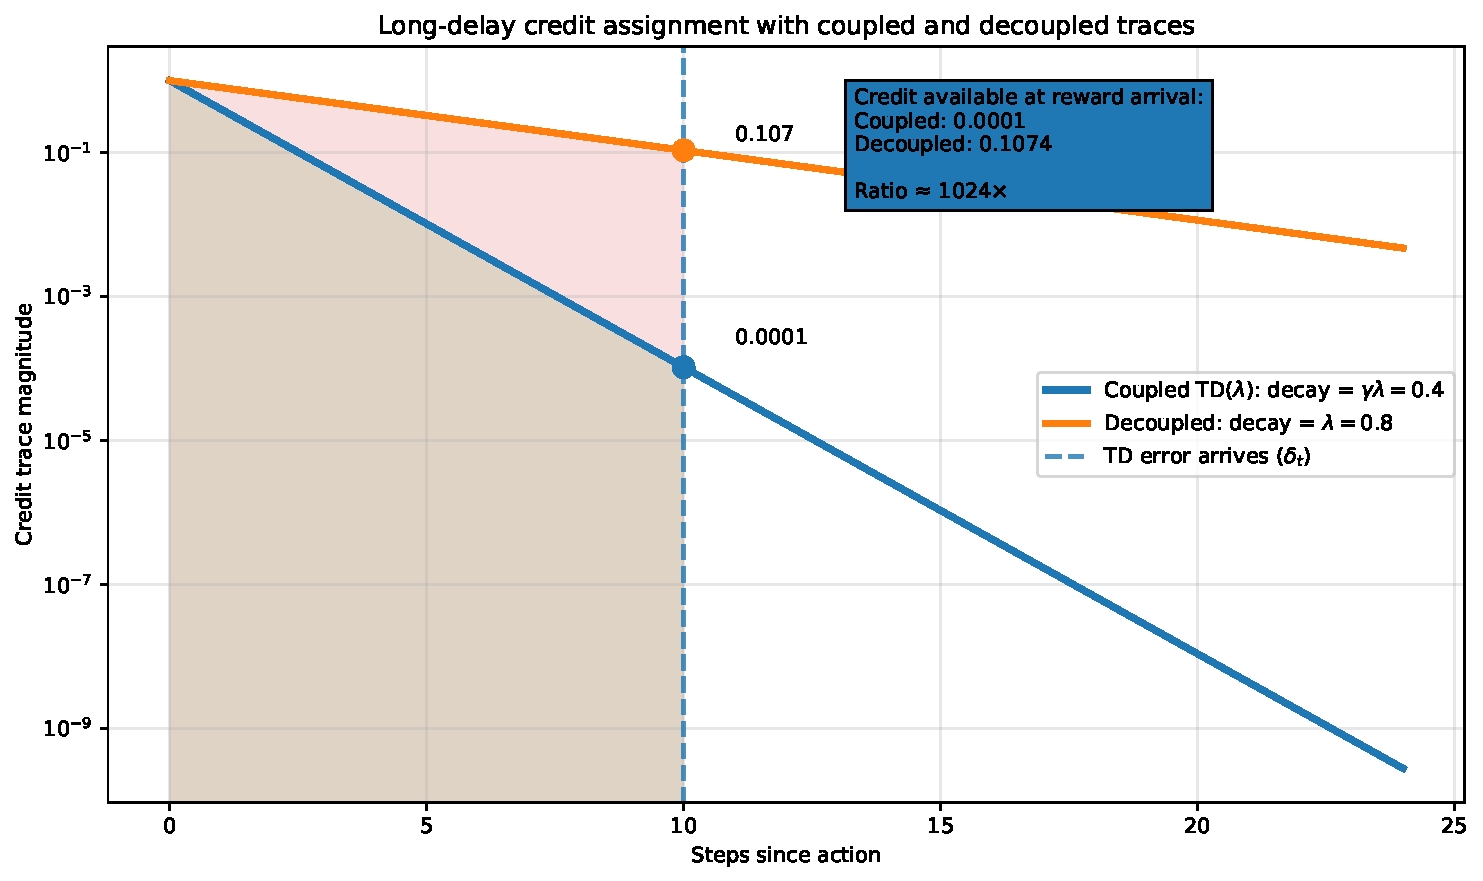
\includegraphics[width=0.45\linewidth]{images/credit_trace_comparison.pdf}
    \caption[Coupled vs.\ decoupled $\gamma
    ;\lambda$ credit traces]{Effect of coupling and decoupling $\gamma$ and $\lambda$ on temporal credit assignment. The figure shows the evolution of a credit trace following a single contribution at $t=0$. In the standard $TD(\lambda)$ formulation, the trace decays with factor $\gamma\lambda$, whereas in the proposed formulation it decays with factor $\lambda$ alone. For $\gamma=0.5$ and $\lambda=0.8$, the coupled trace rapidly approaches zero, leaving little credit available when a delayed TD error is observed. Decoupling the trace from the critic discount factor preserves a longer credit-assignment horizon while retaining the shorter value-estimation horizon required for stable learning.
    }
    \label{fig:gamma-lambda-decoupling-visualization}
\end{figure}

\subsection{Implementation in Multi-Step Action Windows}
\label{sec:multi-step-action}

The preceding discussion treats $\gamma$ and $\lambda$ as quantities defined at
the behavioral level, i.e. per agent action. In the simulations used in this
work, however, each action is maintained for $\Delta$ neural integration
steps. The corresponding per-step decay constants are therefore obtained by

\begin{equation}
\gamma_{\mathrm{step}} = \gamma^{1/\Delta},
\qquad
\lambda_{\mathrm{step}} = \lambda^{1/\Delta},
\end{equation}
so that the effective discount and credit-assignment horizons remain unchanged
when measured in units of actions.

Throughout the experiments we use $\gamma = 0.5$ and $\lambda = 0.8$ at the
action level. This choice reflects the role separation introduced above. A
relatively small $\gamma$ helps stabilize value learning in the continuous,
non-episodic spiking setting by limiting the critic's bootstrap horizon,
whereas a larger $\lambda$ preserves a substantially longer action-credit
window. Under the conventional coupling, the effective actor trace would decay
with $\gamma\lambda = 0.4$, producing a much shorter memory of past
action-related contributions. By decoupling the two constants, the critic can
remain short-horizon and stable while the actor continues to assign credit
across longer delays between actions and their consequences.

This modification should be viewed as a pragmatic design choice for online
spiking reinforcement learning, and shouldn't be seen as an exact implementation of
standard TD($\lambda$). Its motivation is to preserve useful long-range credit
assignment in regimes where critic stability requires strong discounting, and
its validity is ultimately assessed through the empirical results presented in
later chapters.


% ─────────────────────────────────────────────────────────────

\section{Distributed E-prop}
\label{sec:distributed_eprop}

The second contribution of this work is distributed e-prop, a learning rule that eliminates the need for structured feedback weights. Each neuron evaluates
its own contribution to the global outcome using only the broadcasted TD error $\delta_t$,
with no neuron-specific gradient routing.

   \subsection{Introduction: A Distributed View of Policy Optimization}
    \label{sec:distributed_eprop_intuition}
    
    Before presenting the formal derivation, it is helpful to situate distributed e-prop
    within a broader landscape of optimization strategies, and in particular to contrast it
    with the family of methods that backpropagation and standard e-prop belong to. This
    contrast motivates both the name and the design choices that follow.
    
    Backpropagation and its online approximations, including standard e-prop, share a common
    requirement: in order to update a parameter, the algorithm must know how that parameter
    influences the policy, that is, how the probability distribution over actions would
    change if that parameter were modified. In the policy gradient framework, this is
    captured by the score function $\nabla_\theta \log \pi(a \mid s; \theta)$, which
    measures the sensitivity of the log-probability of the selected action to each parameter.
    In backpropagation this quantity is computed by propagating gradients backward through
    the full network graph. In standard e-prop it is approximated by routing a
    neuron-specific signal back to each hidden neuron through feedback weights $B_{kj}^\pi$,
    so that each synapse receives an estimate of how its activity contributes to changing
    what the agent does. Note that the task signal, in the form of the temporal-difference
    error $\delta_t$, is present in both standard e-prop and distributed e-prop, it is not what distinguishes the two approaches. What distinguishes them is whether each parameter
    also receives structural information about how it influences the policy. It is precisely
    this structural signal, the approximation of $\nabla_\theta \log \pi$ routed back
    through the network, that distributed e-prop eliminates.
    
    A fundamentally different philosophy exists, one that abandons this structural accounting
    entirely and replaces it with a much simpler question: \emph{Was the outcome better or worse than expected, and what did I try?} This is the intuition behind evolutionary and
    perturbation-based optimisation methods such as genetic algorithms and evolution
    strategies~\cite{salimans2017evolutionstrategiesscalablealternative}. In these methods, candidate solutions are
    perturbed randomly, the resulting outcomes are evaluated, and perturbations that led to
    improvements are reinforced. No parameter needs to know how it influences the output
    through the network; it only needs to remember what perturbation it applied and whether
    the global outcome improved. The update rule is simply the product of the scalar outcome
    signal, shared identically across all parameters, and the local perturbation, which each
    parameter already knows because it generated it. The structural question of how each
    parameter shapes the policy is never asked; it is replaced by the empirical question of
    whether trying something different locally happened to coincide with a better outcome.
    
    Distributed e-prop is built on this same philosophy, adapted to work online and in
    continuous time within a recurrent spiking network. The key conceptual step is to treat
    each neuron not merely as a processing unit within a single global policy, but as an
    independent stochastic actor with its own local policy over its membrane dynamics.
    Concretely, each neuron $j$ maintains a Gaussian policy over its own membrane potential $v_j^t$, drawing a small
    random perturbation at each timestep and treating it's perturbed membrane as its local action.
    The spike train that results from those perturbed membrane dynamics constitutes the
    observable behavior that the perturbation produces, and it is through this behavior
    that the neuron influences the global outcome. In this sense the global agent policy
    emerges from the collective behavior of many small independent actors, each exploring
    locally, rather than from a single centralized computation whose gradient is then routed
    back to every parameter.
    
    Because the neurons integrate their inputs over time, a perturbation applied at time $t$ does
    not simply affect the membrane instantaneously and then vanish, its residual influence decays
    through the membrane dynamics over subsequent timesteps. Each neuron therefore maintains
    a filtered trace $\xi_j^t$ that accumulates the effect of its past perturbations on its
    current membrane state, decaying at the same rate $\alpha$ as the membrane itself. This
    trace serves as the neuron's local memory of what it has been trying recently, playing
    the same role that the stored perturbation plays in the static ES setting, but extended
    across time. When the global temporal-difference error $\delta_t$ arrives, each neuron
    uses its own $\xi_j^t$ to assess whether what it was trying recently contributed to the
    outcome being better or worse than expected, and updates its incoming weights accordingly.
    Crucially, \emph{no approximation of $\nabla_\theta \log \pi$ is needed at any point}, the
    structural question of how each neuron shapes the policy is replaced entirely by the
    empirical evidence accumulated in $\xi_j^t$.

    A natural question at this point is why this approach should work at all. If every
    parameter is being perturbed simultaneously, the change in the global outcome reflects
    the combined effect of thousands of simultaneous perturbations with residual influence over time, so attributing any part
    of that change to a single synapse seems hopeless. This concern is well founded, weight perturbation methods are known to suffer from variance that grows
    linearly with the number of parameters, precisely because every other perturbation
    contributes noise to the gradient estimate of each individual weight. The reason
    distributed e-prop can nevertheless be expected to produce a useful learning signal lies
    in two complementary mechanisms.
    
    The first is statistical. Even when all parameters are perturbed simultaneously, the
    expected value of the update for any single synapse $W_{ji}$ is still the correct
    gradient, because the perturbations of all other synapses are independent and
    zero-mean, and their contributions therefore cancel in expectation. What remains after
    averaging over many updates is the true gradient signal, sitting on top of noise whose
    magnitude is large but whose mean is zero. In this sense the law of large numbers is
    doing the essential work, no single update is reliable, but the correct direction
    accumulates steadily over time while the noise averages away.
    
   The second mechanism is structural, and it is what makes distributed e-prop
    qualitatively different from naive simultaneous perturbation. The core perturbation
    estimator already contains a natural credit assignment structure through the presynaptic
    activity, which conditions each synaptic update on whether neuron $i$ was recently
    active and therefore in a position to have contributed to the membrane state that the
    perturbation acted on. The single heuristic addition on top of this is the surrogate
    derivative $\psi_j^t$, which focuses credit further by weighting updates according to
    how close the postsynaptic neuron was to its firing threshold at each moment. The
    intuition is that a perturbation that occurs when the membrane is far from
    threshold is unlikely to have changed the spike output, and therefore unlikely to have
    influenced the global outcome, so it should receive little credit. Multiplying by
    $\psi_j^t$ implements exactly this reweighting, and the product of $\psi_j^t$ with the
    presynaptic activity is precisely the eligibility trace $e_{ji}^t$. This single
    heuristic introduction dramatically reduces the effective variance of the estimator at
    the cost of bias, and it is what makes the rule stable enough to operate online in
    a single continuous trajectory without requiring the large parallel populations that
    unbiased perturbation methods need.
    
    No neuron requires a centrally computed policy gradient, and no structured information
    about how the global policy depends on each parameter needs to be routed back through
    the network. The local signals that each neuron constructs can still propagate to other
    neurons, as in the backpropagated variants described in
    Section~\ref{subsec:structured_routing}, but their origin is always local and perturbation-based. The policy is in this
    sense distributed as it emerges from the independent stochastic behavior of many
    individual actors, each optimizing itself against the same shared scalar signal
    $\delta_t$.

    A final important observation concerns the role of the output weights. Throughout the
    recurrent and hidden layers, the weight updates are driven by noisy perturbation-based
    estimates that are only correct in expectation and over many steps. The output weights,
    by contrast, receive an exact gradient at every step, since the readout is a linear
    non-recurrent transformation and no approximation of the kind introduced by e-prop is
    needed there. The output weights are responsible for
    aggregating the activity of the hidden population into a value estimate and a policy
    signal, and it is the quality of this aggregation that determines how informative and
    stable the temporal-difference error $\delta_t$ is for the recurrent layer. Without the
    output weights learning a meaningful readout, $\delta_t$ would be extremely noisy,
    making it far harder for the perturbation correlations in the hidden layer to accumulate
    into a useful learning signal. Furthermore, if the output weights were fixed, the
    recurrent neurons would face a significantly harder problem, instead of the readout
    adapting to extract whatever structure the recurrent layer naturally develops, each
    hidden neuron would need to organize its activity to match an arbitrary fixed
    projection. Having the output weights learn the aggregation is therefore not merely
    convenient but arguably one of the most important factors in making the perturbation-based
    updates in the recurrent layer feasible. This is analogous to reservoir computing
    \citep{Maass2002LSM}, where a fixed random recurrent network can solve
    tasks because a trained linear readout learns to extract the relevant
    structure from the random recurrent dynamics.
    The key difference is that here the recurrent weights do learn, but the output weights
    play an arguably dominant role (particularly early in training), when the
    hidden representations are still unstructured. The recurrent learning can then be
    understood as a slow refinement of those representations, guided by a task signal whose
    quality depends heavily on how well the output layer has already learned to read them
    out.
    
    The sections that follow make this precise. Section~\ref{subsec:neuron_as_actor} formalises
    the interpretation of each neuron as a stochastic actor, and
    Section~\ref{subsec:lif_update_rule} describes the resulting update rule for LIF and ALIF
    neurons, showing how the perturbation trace $\xi_j^t$ and the e-prop eligibility trace
    $e_{ji}^t$ combine with $\delta_t$ to produce a fully local, online weight update.

    \subsection{Neurons As Stochastic Actors}
    \label{subsec:neuron_as_actor}
    
    As discussed previously, the non-local learning signal $L_j^t$ used in standard
    reward-based e-prop introduces an approximation to the true gradient, since
    estimating the contribution of each neuron to the global objective requires
    information about downstream network dynamics.
    One alternative is to reinterpret each neuron as an independent stochastic
    actor interacting with the rest of the recurrent network as its environment.
    Under this interpretation, learning can be performed using only local neuron
    dynamics, local stochastic exploration, and a globally broadcast evaluative
    signal.
    
    Instead of treating spikes themselves as stochastic actions, stochasticity is
    introduced directly into the membrane dynamics by treating the membrane
    potential as a stochastic actor.
    The emitted spikes remain deterministic threshold events.
    For each neuron $j$, the membrane potential is drawn from a Gaussian policy
    \[
        v_j^t \sim \mathcal{N}(\mu_j^t,\, \sigma_j^2),
    \]
    where $\mu_j^t$ is the unperturbed membrane state determined by the
    deterministic dynamics, and $\sigma_j^2$ is a per-neuron exploration variance.
    We write $\varepsilon_j^t = v_j^t - \mu_j^t$ for the additive perturbation,
    so that $\varepsilon_j^t \sim \mathcal{N}(0, \sigma_j^2)$.
    Under this formulation, the stochastic policy is defined over membrane
    trajectories.
    The perturbations therefore play the role of exploratory actions, while the
    resulting spike trains constitute the observable behavior generated by those
    actions.
    
    A key distinction from standard policy-gradient formulations is that the
    membrane potential itself is not directly observable by downstream neurons or
    by the environment.
    The observable quantity is instead the emitted spike train
    \[
        z_j^t = H(v_j^t - v_{\mathrm{th}}),
    \]
    where $H$ denotes the Heaviside Step function.
    Consequently, membrane perturbations only influence behavior insofar as they
    modify spike timing.
    
    \subsection{The Update Rule for LIF Neurons}
    \label{subsec:lif_update_rule}
    
    We first consider a network of leaky integrate-and-fire (LIF) neurons.
    The perturbed membrane dynamics are
    \[
        v_j^{t+1} = \alpha v_j^t + \sum_i W_{ji}\, z_i^t - z_j^t\, v_{\mathrm{th}}
                    + \varepsilon_j^t,
    \]
    where $\alpha$ is the membrane decay constant.
    The perturbation $\varepsilon_j^t$ enters additively into the membrane at each
    step, and its residual influence on the membrane at subsequent times decays at
    the same rate $\alpha$ as the membrane itself.
    We capture this accumulated influence by the filtered perturbation trace
    \[
        \xi_j^t = \alpha\, \xi_j^{t-1} + \varepsilon_j^t,
    \]
    so that $\xi_j^t$ represents the total contribution of all past perturbations
    to the current membrane state.
    
    The weight update is derived by correlating the local perturbation with the
    global return signal, following the evolution strategies approach.
    The score function of the Gaussian policy with respect to the mean $\mu_j^t$
    is $\varepsilon_j^t / \sigma_j^2$, which after temporal filtering gives
    $\xi_j^t / \sigma_j^2$.
    Chaining through $\partial \mu_j^t / \partial W_{ji} = \epsilon_{ji}^{t,v}$,
    the presynaptic eligibility vector, yields the gradient estimate
    \[
        \nabla_{W_{ji}} J
        \approx
        \mathbb{E}\!\left[
            \delta_t \cdot
            \frac{(1 - \alpha^2)\,\xi_j^t}{\sigma_j^2} \cdot
            \epsilon_{ji}^{t,v}
        \right],
    \]
    where $(1-\alpha^2)$ normalises for the stationary variance of the filtered
    perturbation process and $\delta_t$ is the broadcast TD error.
    
    This estimator correlates membrane perturbations with reward regardless of
    whether those perturbations actually caused a spike.
    A natural refinement is to weight the update by the sensitivity of the spike
    output to the membrane state, focusing credit on perturbations that were near
    threshold and thus likely to have modified spike timing.
    We therefore introduce $\psi_j^t$, the surrogate derivative of $H$ at
    $v_j^t$, as a heuristic modulation of the update: it is large near threshold
    and suppresses updates when the neuron is far from firing.
    Incorporating this term and recognising that $\psi_j^t \cdot \epsilon_{ji}^{t,v}$
    is precisely the e-prop eligibility trace $e_{ji}^t$ for LIF
    neurons~\cite{eprop2020}, the full update rule becomes
    \[
        \Delta W_{ji}
        \propto
        \delta_t\;
        \mathcal{F}_{\lambda}
        \!\left(
            \frac{(1 - \alpha^2)\, \xi_j^t}{\sigma_j^2}\;
            e_{ji}^t
        \right),
    \]
    where $\mathcal{F}_{\lambda}$ is a low-pass filter that accumulates credit
    over time.
    We note that the $\psi_j^t$ modulation is a choice,
    one could use the estimator without it, or apply other gating mechanisms (perhaps smoother functions), yielding
    valid alternative variants of the update rule, but, as it will be shown in Chapter~\ref{ch:results} this gating becomes essential for the rule to function properly.
    
    \paragraph{Extension to ALIF neurons.}
    For adaptive leaky integrate-and-fire (ALIF) neurons, the firing threshold
    depends on the neuron's recent spiking history through an adaptation variable
    $a_j^t$, giving the spike condition $z_j^t = H(u_j^t)$ where $u_j^t =
    v_j^t - A_j^t$ and $A_j^t = v_{\mathrm{th}} + \beta_j a_j^t$ is the adaptive
    threshold.
    The actor remains $v_j^t$, with the perturbation $\varepsilon_j^t$ injected
    into the membrane as before.
    The ES estimator is unchanged, still giving $\xi_j^t / \sigma_j^2 \cdot
    \epsilon_{ji}^{t,v}$ from the policy gradient.
    However, the e-prop framework also provides access to $\epsilon_{ji}^{t,a}$,
    the eligibility vector tracking the sensitivity of the adaptive threshold to
    $W_{ji}$ through the spiking history.
    Applying the same $\psi_j^t$ heuristic and extending it to include the
    adaptation contribution (which is natural since $\psi_j^t$ acts on $u_j^t =
    v_j^t - A_j^t$ and both membrane and adaptation dynamics feed into it) gives
    $\psi_j^t \cdot (\epsilon_{ji}^{t,v} + \epsilon_{ji}^{t,a})$, which is
    precisely the e-prop eligibility trace $e_{ji}^t$ for ALIF
    neurons~\cite{eprop2020}.
    The update rule therefore retains exactly the same form with $e_{ji}^t$
    reinterpreted accordingly.
    Including $\epsilon_{ji}^{t,a}$ is again a heuristic choice, one could omit
    it and use only $\epsilon_{ji}^{t,v}$, or include it with a different
    weighting, producing a family of possibly functional variants.
    
    \subsection{Intuitive Justification for the Eligibility Trace}
    \label{subsec:etrace_intuition}
    
    The update rule derived above combines three factors, $\delta_t$,
    $\xi_j^t / \sigma_j^2$, and $e_{ji}^t$, each playing a distinct and
    complementary role in local credit assignment.
    This section unpacks that decomposition to provide an intuitive justification
    for the use of the eligibility trace, independent of the heuristic argument
    that led to it.
    
    The TD error $\delta_t$ is a scalar signal broadcast uniformly to all neurons.
    It evaluates whether the global outcome was better or worse than expected under
    the current policy, and provides the evaluative signal that determines the sign
    and magnitude of all weight updates.
    It carries no information about which neurons or synapses were responsible for
    that outcome.
    
    The perturbation trace $\xi_j^t$ fills a different role entirely.
    It accumulates the causal footprint of past exploration noise on the current
    membrane state of neuron $j$, specifically how much the perturbations have
    cumulatively shifted the membrane away from what the deterministic dynamics
    alone would have produced, and in which direction.
    A large positive $\xi_j^t$ means the membrane has been pushed upward by
    recent noise; a large negative value means it has been pushed downward.
    Crucially, $\xi_j^t$ carries no evaluative content and does not encode whether
    those shifts were beneficial.
    That judgment is left entirely to $\delta_t$.
    Together, $\delta_t \cdot \xi_j^t / \sigma_j^2$ answers the question of whether
    the perturbations that drove this neuron's membrane in a given direction were
    followed by better or worse outcomes than expected.
    
    What remains is the question of which synapses should be updated in response.
    The perturbation entered through the membrane, and the membrane is a sum of
    contributions from all incoming synapses, so the perturbation's effect on the
    spike output was mediated by the same membrane dynamics that all synapses share.
    The eligibility trace $e_{ji}^t = \psi_j^t \cdot \epsilon_{ji}^{t,v}$ (or
    its ALIF counterpart $\psi_j^t \cdot (\epsilon_{ji}^{t,v} +
    \epsilon_{ji}^{t,a})$) provides the answer.
    It measures the sensitivity of the neuron's recent spike output to the
    synaptic weight $W_{ji}$, accumulated over time through the membrane dynamics,
    asking how much the spike activity of neuron $j$ would have differed if
    $W_{ji}$ had been slightly different.
    A synapse with large $|e_{ji}^t|$ was highly influential in shaping the
    membrane state that determined whether the perturbation produced a spike, while
    a synapse with small $|e_{ji}^t|$ had little influence, perhaps because the
    presynaptic neuron was silent or the membrane was far from threshold.
    
    The full update $\delta_t \cdot \xi_j^t / \sigma_j^2 \cdot e_{ji}^t$
    therefore has a clean three-factor interpretation. A synapse is strengthened
    or weakened when the global outcome was better or worse than expected
    ($\delta_t$), the membrane was being driven by exploration noise in a
    particular direction ($\xi_j^t$), and that synapse was causally responsible
    for the membrane state being sensitive to the spike output at that moment
    ($e_{ji}^t$).
   
    This structure is similar to the three-factor rules proposed in biological
    models of reward-modulated synaptic plasticity
    \citep{Fremaux2016NeuromodulatedSTDP}, where a neuromodulatory signal
    gates a Hebbian-like trace formed from correlated pre- and postsynaptic
    activity. The eligibility trace $e^t_{ji}$ inherited from standard e-prop
    plays exactly this role, and concrete biological instances of a global
    signal gating such as traces predate e-prop by over a decade
    \citep{Izhikevich2007DistalReward,Florian2007RewardSTDP}. The perturbation
    trace $\xi^t_j$ has no comparable precedent in this literature, since
    classical reward-modulated STDP rules do not model exploration as
    injected continuous noise; the closer biological precedent for this
    component is the conductance-fluctuation models of \citep{fiete2006gradient}, in which a REINFORCE-like estimator emerges directly
    from injected noise.
    
    \subsection{Synaptic Perturbation Variants}
    \label{subsec:synaptic_perturbation}
    
    The formulation above treats each neuron as a stochastic actor, injecting a shared
    membrane perturbation $\varepsilon_j^t$ that affects all incoming synapses
    simultaneously. This neuron perturbation variant has a natural bias-variance
    interpretation, that is because a single noise source is shared across all incoming synapses of
    neuron $j$, the gradient estimate for each individual synapse $W_{ji}$ is contaminated
    by the contributions of all other synapses to the membrane, since all of them
    experienced the same perturbation. The estimator cannot distinguish which synapse was
    responsible for the membrane shift; it only knows that the neuron as a whole was
    perturbed. This introduces bias into the per-synapse credit assignment, but keeps the
    number of independent noise sources equal to the number of neurons, which limits
    variance.
    
    A natural alternative is to push the stochasticity one level lower and treat each
    synapse as an independent actor. Rather than perturbing the membrane directly, a
    separate noise term $\varepsilon_{ji}^t \sim \mathcal{N}(0, \sigma_{ji}^2)$ is added
    to the synaptic transmission, so that the membrane dynamics become
    \[
        v_j^{t+1}
        =
        \alpha v_j^t
        +
        \sum_i \bigl(W_{ji} + \varepsilon_{ji}^t\bigr) z_i^t
        -
        z_j^t v_{\mathrm{th}}.
    \]
    The effective membrane perturbation produced by synapse $ji$ at time $t$ is therefore
    $\varepsilon_{ji}^t z_i^t$: the noise is only injected into the membrane when the
    presynaptic neuron fires. We define a per-synapse perturbation trace
    \[
        \xi_{ji}^t = \alpha\, \xi_{ji}^{t-1} + \varepsilon_{ji}^t z_i^t,
    \]
    which accumulates the residual influence of past synaptic perturbations on the current
    membrane potential, decaying at the same rate $\alpha$ as the membrane itself.
    
    Correlating the synaptic perturbation with the global return, the policy gradient with
    respect to $W_{ji}$ yields
    \[
        \nabla_{W_{ji}} J
        \approx
        \mathbb{E}\!\left[
            \delta_t \cdot
            \frac{(1 - \alpha^2)\, \xi_{ji}^t}{\sigma_{ji}^2}
            \; e_{ji}^t
        \right],
    \]
    where the eligibility trace $e_{ji}^t$ is introduced by the same heuristic argument as
    in the neuron variant. The resulting update rule is
    \[
        \Delta W_{ji}
        \propto
        \delta_t\;
        \mathcal{F}_{\lambda}
        \!\left(
            \frac{(1 - \alpha^2)\, \xi_{ji}^t}{\sigma_{ji}^2}\;
            e_{ji}^t
        \right).
    \]
    This variant resolves the bias of the neuron perturbation estimator: each synapse now
    has its own independent noise source and its own perturbation trace, so the gradient
    estimate for $W_{ji}$ depends only on the perturbation that synapse $ji$ itself
    introduced. However, this comes at the cost of a substantial increase in variance.
    The number of independent noise sources now scales with the number of synapses, which is typically one to two orders of magnitude larger.
    Each synapse contributes its own noise to the shared membrane potential of its
    postsynaptic neuron, and this noise affects the gradient estimates of all other synapses
    onto the same neuron.
    
    \paragraph{Shared postsynaptic noise with per-synapse structure.}
    
    A third variant addresses this variance problem by combining the strengths of the two
    approaches above. Rather than drawing an independent noise sample per synapse, a single
    noise term $\varepsilon_j^t \sim \mathcal{N}(0, 1)$ is drawn per postsynaptic neuron
    $j$ at each timestep, shared across all synapses that project onto $j$ and fire at time
    $t$. However, each synapse $ji$ scales this shared noise by its own per-synapse standard
    deviation $\sigma_{ji}$, so that the effective perturbation contributed by synapse $ji$
    is
    \[
        \varepsilon_{ji}^t z_i^t = \sigma_{ji}\, \varepsilon_j^t\, z_i^t.
    \]
    The per-synapse perturbation trace is then
    \[
        \xi_{ji}^t = \alpha\, \xi_{ji}^{t-1} + \sigma_{ji}\, \varepsilon_j^t\, z_i^t,
    \]
    and the update rule retains the same per-synapse structure as the fully independent
    variant:
    \[
        \Delta W_{ji}
        \propto
        \delta_t\;
        \mathcal{F}_{\lambda}
        \!\left(
            \frac{(1 - \alpha^2)\, \xi_{ji}^t}{\sigma_{ji}^2}\;
            e_{ji}^t
        \right)
    \]
    This variant can be understood as interpolating between the neuron and synaptic
    perturbation extremes. The noise originates at the postsynaptic neuron, as in the
    neuron perturbation variant, which limits the number of independent noise sources to
    the number of neurons and keeps variance under control. At the same time, each synapse
    retains its own $\sigma_{ji}$, so the effective perturbation magnitude is synapse-specific
    and the update structure remains fully per-synapse. The coupling of all synapses onto
    neuron $j$ through the shared $\varepsilon_j^t$ means that the noise simultaneously
    probes the contribution of all active presynaptic neurons at time $t$, testing whether
    their joint activity in the context of this particular postsynaptic neuron was
    beneficial, while the per-synapse $\sigma_{ji}$ and $z_i^t$ factors ensure that the
    resulting gradient estimate is still attributed individually to each synapse. This
    combination appears to offer the best empirical performance of the three variants, which
    we verify in the experimental results of Chapter~\ref{ch:results}.
    
    \subsection{Structured Routing of Local Policy Gradients}
    \label{subsec:structured_routing}
    
    The distributed rules derived so far use a purely global evaluative signal:
    all neurons receive the same broadcast TD error $\delta_t$, while credit
    assignment is performed locally through the perturbation traces and
    eligibility traces.
    This already defines a valid distributed perturbation-based learning rule.
    However, once each neuron is interpreted as a stochastic actor, the local
    perturbation estimator also defines a neuron-local policy-gradient signal.
    This makes it possible to reuse the structured credit-routing machinery of
    symmetric reward-based e-prop~\cite{eprop2020}.
    
    In standard reward-based e-prop, the learning signal routed back to neuron
    $j$ is formed by propagating output error gradients backward through the
    output weights.
    The perturbation-based formulation provides an analogous quantity: a local
    estimate of the policy gradient at each neuron, which can replace the
    externally computed output gradient in the symmetric e-prop routing mechanism.
    Here, since all synapses in the recurrent layer are treated symmetrically,
    the routing proceeds through the recurrent weights themselves, with no
    distinction between output and recurrent connections.
    
    For the neuron perturbation variant, the perturbation trace
    $\xi_j^t / \sigma_j^2$ defines the local stochastic policy-gradient estimator
    associated with neuron $j$.
    Applying the surrogate derivative $\psi_j^t$ yields the neuron-local policy
    signal
    \[
        g_j^t
        =
        \frac{(1-\alpha^2)\,\xi_j^t}{\sigma_j^2}\,
        \psi_j^t,
    \]
    which is then propagated backward through the recurrent weights, aggregating
    feedback from all postsynaptic neurons:
    \[
        L_j^t
        =
        \sum_{k}
        W_{kj}\,
        g_k^t.
    \]
    The resulting synaptic update takes the standard reward-based e-prop form
    \[
        \Delta W_{ji}
        \propto
        -\eta
        \sum_t
        \delta_t\,
        \mathcal{F}_{\lambda}
        \!\left(
            L_j^t\;
            e_{ji}^t
        \right),
    \]
    where the learning signal $L_j^t$ is shared across all incoming synapses of
    neuron $j$.
    
    In the synaptic perturbation variant, the local perturbation estimator exists
    at the level of each individual synapse, with $\xi_{ji}^t / \sigma_{ji}^2$
    serving as the per-synapse analogue of the neuron-level trace $\xi_j^t /
    \sigma_j^2$.
    Instead of aggregating these traces at the postsynaptic neuron before routing,
    the policy signal is formed directly at the synapse.
    This is consistent with the interpretation of $\varepsilon_{ji}^t z_i^t$ as a
    membrane perturbation for which synapse $ji$ is the sole culprit: just as the
    neuron perturbation $\varepsilon_j^t$ is a shared membrane push attributed to
    all incoming synapses jointly, the synaptic perturbation $\varepsilon_{ji}^t
    z_i^t$ is a membrane push attributed exclusively to a single synapse. Applying the surrogate derivative $\psi_j^t$ yields the synapse-local policy
    signal
    \[
        g_{ji}^t
        =
        \frac{(1-\alpha^2)\,\xi_{ji}^t}{\sigma_{ji}^2}\,
        \psi_j^t,
    \]
    which is then propagated backward through the recurrent weights, aggregating
    feedback from all postsynaptic neurons:
    \[
        L_{j}^t
        =
        \sum_{k}
        W_{kj}\,
        g_{kj}^t.
    \]
    The synaptic update therefore becomes
    \[
        \Delta W_{ji}
        \propto
        -\eta
        \sum_t
        \delta_t\,
        \mathcal{F}_{\lambda}
        \!\left(
            L_{j}^t\;
            e_{ji}^t
        \right).
    \]
    The key distinction from the neuron variant is that the policy signal $g_{ji}^t$
    is specific to each synapse through $\xi_{ji}^t$. The aggregation over postsynaptic neurons
    through the recurrent weights remains, as it does in the neuron variant.
    
    In both perturbation variants, the final update rule is identical in form to
    symmetric reward-based e-prop, a neuron-level or synapse-level learning signal
    is routed backward through the recurrent weights, multiplied by the eligibility
    trace $e_{ji}^t$, and modulated by the global TD error $\delta_t$.
    In standard e-prop, $L_j^t$ depends on externally supplied output gradients.
    Here, the learning signal is instead constructed internally from local
    perturbation-based policy-gradient estimates generated independently by each
    neuron or synapse.
    The framework therefore replaces explicit gradient feedback with distributed
    stochastic policy signals derived entirely from local dynamics and a globally
    broadcast evaluative signal.

    A natural extension of the structured routing variants described above is to incorporate
    an additional term into the noise reward trace that draws a more explicit analogy with
    backpropagation. Recall that the neuron-local policy signal $g_j^t$ and its backrouted
    aggregate $L_j^t = \sum_k W_{kj} g_k^t$ are already defined above. Incorporating $L_j^t$
    into the noise reward trace gives
    \begin{equation}
        p_{ji}^{\xi, t} = \lambda \, p_{ji}^{\xi, t-1}
        + e_{ji}^t \left(g_j^t + g_j^tL_j^t \right),
        \label{eq:rl_noise_trace_extended}
    \end{equation}
    
    where the additional term $e_{ji}^t g_j^t L_j^t$ modulates the update by
    the degree of agreement between the local policy signal of neuron $j$ and the
    backrouted aggregate of postsynaptic policy signals. When the two are aligned, the
    synapse receives a stronger update, since the local perturbation propagated its effect
    forward through the recurrent connections in a direction consistent with the
    perturbation activity of downstream neurons. When they disagree, the term attenuates
    the update. There is a clear connection with backpropagation and the chain rule, but, here it is used as a heuristic term, as it does not appear from the derivation. It can be seen as a variance reduction term, that focuses the updates on synchronized perturbations.
    
    \begin{figure}[H]
        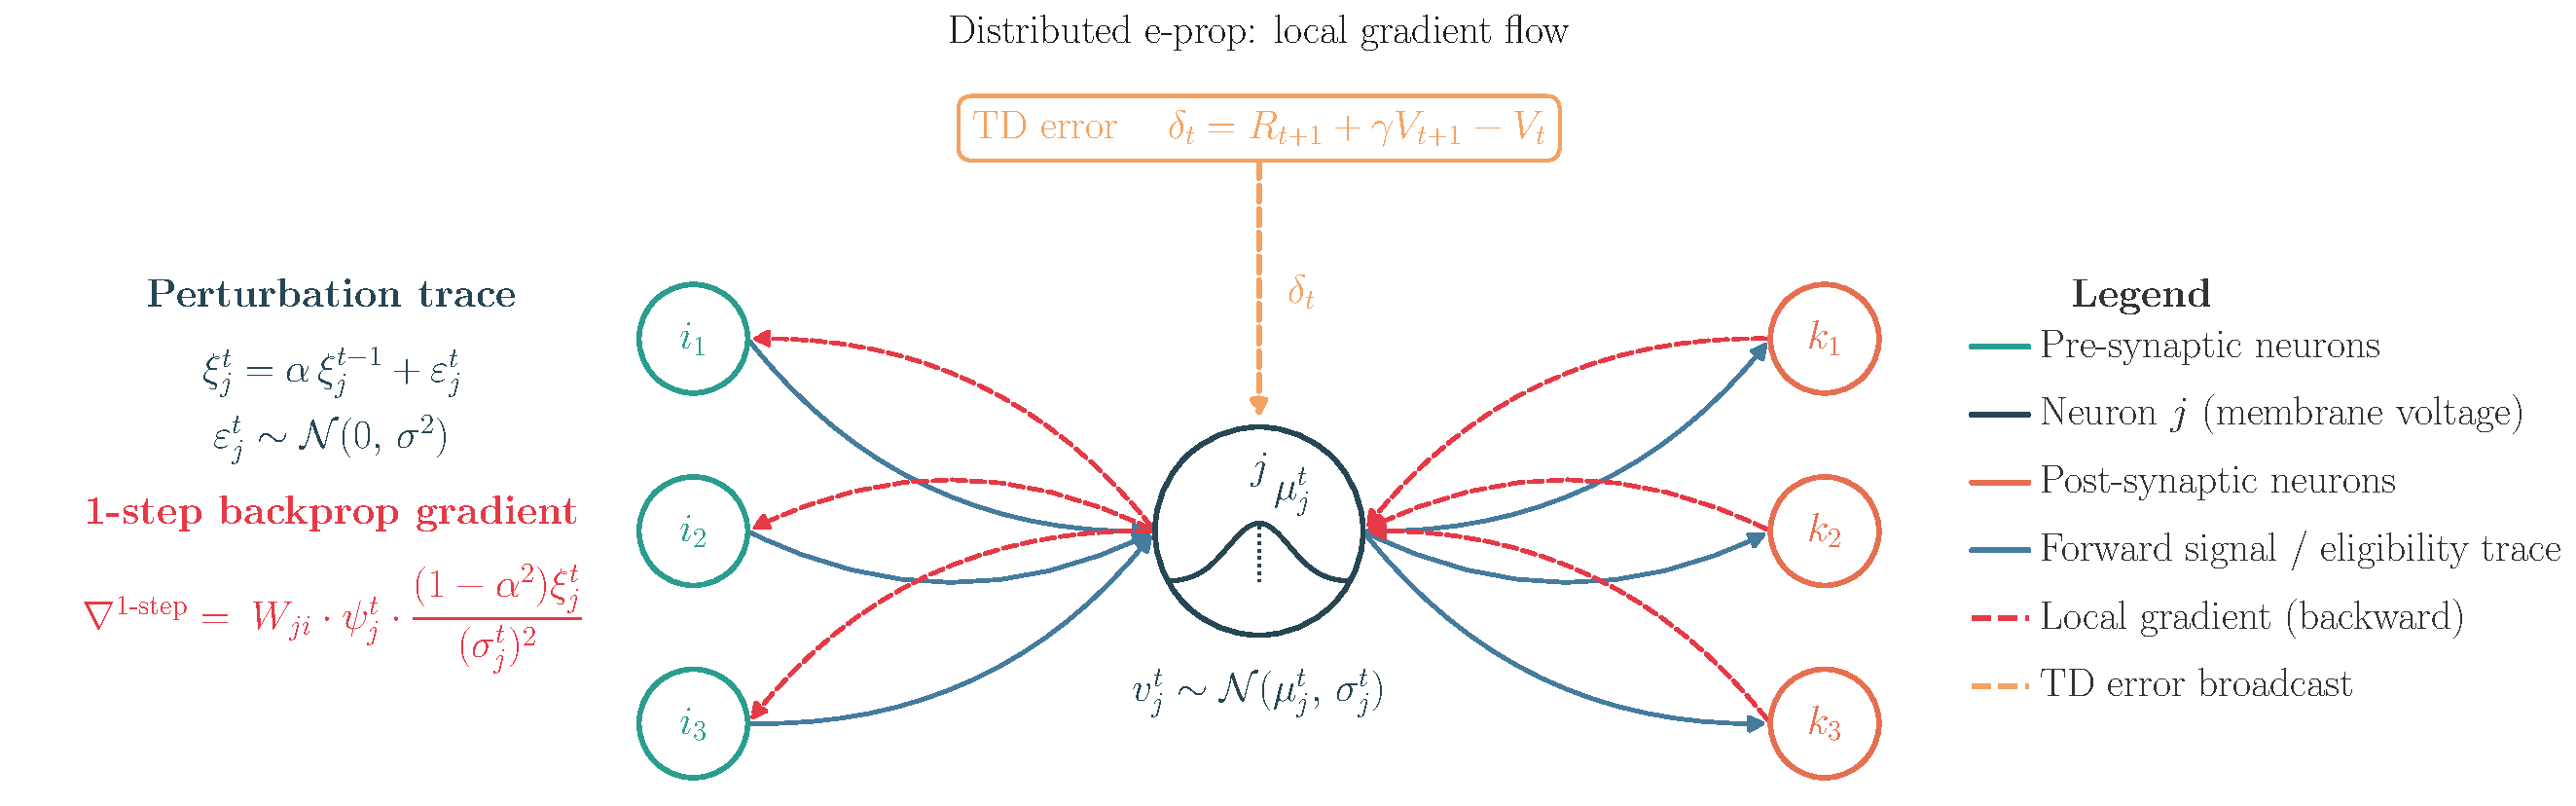
\includegraphics[width=1.0\linewidth]{images/distributed_eprop_diagram.pdf}
        \caption[Local gradient flow in distributed e-prop]{\textbf{Local gradient flow in the 1-step backpropagated distributed
        e-prop algorithm.}
        Neuron $j$ maintains an internal membrane voltage
        $v_j^t \sim \mathcal{N}(\mu_j^t, \sigma_j^t)$
        (represented by the Gaussian curve) and receives
        perturbation-based input from pre-synaptic neurons $i_1$--$i_3$
        (teal, left).
        The perturbation trace
        $\xi_j^t = \alpha\,\xi_j^{t-1} + \varepsilon_j^t$
        accumulates the stochastic exploration signal along each incoming
        synapse (blue arcs).
        Spikes $z_j^t$ are propagated forward to post-synaptic neurons
        $k_1$--$k_3$ (orange, right).
        A global TD error
        $\delta_t = R_{t+1} + \gamma V_{t+1} - V_t$
        is broadcast to the neuron from an external critic
        (orange dashed arrow).
        The 1-step backpropagation variant sends the local gradient information to their respective presynaptic neurons.
        }
        \label{fig:distributed_eprop}
    \end{figure}

    \clearpage
    \subsection{Exploration Variance \texorpdfstring{$\sigma$}{sigma}}
    \label{subsec:exploration_variance}
    
    The perturbation variance $\sigma_j^2$ controls the amount of local
    exploration performed by each neuron and plays a role analogous to the step
    size in stochastic search methods.
    Its choice has a direct effect on the bias-variance tradeoff of the gradient
    estimate: large $\sigma_j$ increases exploration but adds noise to the
    membrane dynamics and degrades network performance, while small $\sigma_j$
    reduces exploration and may prevent learning altogether.
    Three broad approaches can be taken.
    
    A static variance treats $\sigma_j$ as a fixed hyperparameter, either shared
    across all neurons or set individually.
    This avoids any additional learning machinery but requires manual tuning and
    cannot adapt as the policy evolves.
    In particular, a fixed $\sigma_j$ that is appropriate early in training, when
    the network is far from a good policy and wide exploration is beneficial, may
    be too large once a policy has been found and fine-grained exploitation is
    needed.
    A more expressive alternative makes $\sigma_j^t$ a function of the network
    state, for instance by reading it from a dedicated output neuron or by tying
    it to the membrane potential, allowing the network to modulate its own
    exploration in a context-dependent manner at the cost of a more complex
    architecture and additional credit assignment for the parameters governing
    $\sigma_j^t$.
    
    The third, and typically used approach, is to make $\log\sigma_j$ a
    per-neuron learnable scalar updated online by its own policy gradient.
    For the Gaussian policy $v_j^t \sim \mathcal{N}(\mu_j^t, \sigma_j^2)$,
    the score function with respect to $\log\sigma_j$ is
    \[
        \nabla_{\log\sigma_j} \log\pi_j
        =
        \frac{\varepsilon_j^{t\,2}}{\sigma_j^2} - 1,
    \]
    which has expectation zero under the current policy and is positive when the
    observed perturbation is larger than expected, indicating that increasing
    $\sigma_j$ would have been beneficial.
    Replacing the instantaneous perturbation with the filtered trace $\xi_j^t$
    and normalising for the stationary variance of the filtered process gives the
    online estimator
    \[
        s_j^t
        =
        \frac{(1-\alpha^2)\,(\xi_j^t)^2}{\sigma_j^2} - 1,
    \]
    which is accumulated over time and used to update $\log\sigma_j$ via
    \[
        \log\sigma_j
        \leftarrow
        \operatorname{clip}\!\left(
            \log\sigma_j + \eta_\sigma\, \delta_t\, s_j^t,\;
            \log\sigma_{\min},\;
            \log\sigma_{\max}
        \right),
    \]
    where $\eta_\sigma$ is a dedicated learning rate and the clipping enforces
    hard bounds on the exploration range.
    Parameterising in log space ensures $\sigma_j$ remains positive and makes the
    update scale-invariant with respect to the current value of $\sigma_j$.
    The update has an appealing interpretation: when $\delta_t > 0$ the outcome
    was better than expected, so the variance is increased if the perturbation was
    larger than typical (exploration was useful) and decreased otherwise; when
    $\delta_t < 0$ the signs reverse.
    In this way $\sigma_j$ adapts to the local curvature of the reward landscape
    as seen by each neuron independently.
    
    For the synaptic perturbation variant an analogous per-synapse update on
    $\log\sigma_{ji}$ can be defined using $\xi_{ji}^t$ in place of $\xi_j^t$.

    \subsection{Complete Update Rules with TD($\lambda$)}
    \label{subsec:complete_update_rules}
    
    We now consolidate the contributions of this section into a complete set of
    update rules, applying the TD($\lambda$) integration developed in
    Section~\ref{sec:decoupled-lambda-rule} to the distributed e-prop framework. The
    result is a family of fully online, local learning rules of increasing
    complexity, each building on the previous one by adding a new source of
    structured credit assignment. All rules are driven by the same globally
    broadcast TD error
    \begin{equation}
    \delta_t = R_{t+1} + \gamma V_{t+1} - V_t,
    \label{eq:complete-tderror}
    \end{equation}
    and differ only in the local trace that this error modulates.
    
    The value head is trained by standard TD learning. Its eligibility trace decays
    at rate $\gamma$ to remain consistent with the discounted bootstrap target,
    \begin{equation}
    \nu_{ji}^t = \gamma\, \nu_{ji}^{t-1} + \bar{z}_i^t,
    \qquad
    \Delta W_{ji}^V = \eta_V \sum_t \delta_t\, \nu_{ji}^t,
    \label{eq:complete-critic}
    \end{equation}
    where $\bar{z}_i^t$ is the filtered presynaptic spike train.
    
    The weights connecting the hidden population to the policy head are trained by a
    TD($\lambda$) rule whose credit trace accumulates the presynaptic activity
    weighted by the policy-gradient signal,
    \begin{equation}
    p_{ji}^{\pi,t} = \lambda\, p_{ji}^{\pi,t-1}
    + \bar{z}_i^t \, \nabla_{y_k^t} \log \pi^t(a_t),
    \qquad
    \Delta W_{ji}^\pi = \eta_\pi \sum_t \delta_t\, p_{ji}^{\pi,t},
    \label{eq:complete-policy}
    \end{equation}
    where $y_k^t$ are the output logits. The policy-gradient signal is directly
    available at the output head; the trace simply accumulates it over time
    weighted by $\lambda$, after which $\delta_t$ modulates it exactly as for every
    other weight in the network.
    
    The remaining (hidden and recurrent) weights all share a single update form,
    \begin{equation}
    \Delta W_{ji} = \eta \sum_t \delta_t\, p_{ji}^{\,t},
    \qquad
    p_{ji}^{\,t} = \lambda\, p_{ji}^{\,t-1} + c_{ji}^{\,t},
    \label{eq:master-update}
    \end{equation}
    and differ only in the instantaneous credit term $c_{ji}^{\,t}$. Two local
    signals enter these terms: the neuron-local policy signal
    \begin{equation}
    g_j^t = \psi_j^t\,(1-\alpha^2)\,\xi_j^t / \sigma_j^2,
    \label{eq:local-policy-signal}
    \end{equation}
    defined in Section~\ref{subsec:structured_routing}, and its backrouted
    aggregate
    \begin{equation}
    \Lambda_j^t = \sum_k W_{kj}\, g_k^t,
    \label{eq:backrouted-aggregate}
    \end{equation}
    which sums the local policy signals of all postsynaptic neurons weighted by the
    recurrent weights. The backrouted aggregate $\Lambda_j^t$ can enter the update
    in two distinct ways: \emph{additively}, as a separate routing trace, or
    \emph{multiplicatively}, gating the perturbation credit itself. The family of
    rules is obtained by the following choices of $c_{ji}^{\,t}$:
    
    \begin{table}[h]
    \centering
    \renewcommand{\arraystretch}{1.6}
    \begin{tabular}{@{}lll@{}}
    \toprule
    \textbf{Variant} & \textbf{Credit term $c_{ji}^{\,t}$} & \textbf{Decay} \\
    \midrule
    Local perturbation (base)
      & $e_{ji}^t\, g_j^t$
      & $\lambda_\xi$ \\
    \addlinespace
    + structured routing
      & $e_{ji}^t\, g_j^t$ \; and \; $e_{ji}^t\, \Lambda_j^t$ \;(separate trace)
      & $\lambda_\xi,\ \lambda_L$ \\
    \addlinespace
    + gating by structured routing
      & $e_{ji}^t\, g_j^t\,(1 + \Lambda_j^t)$ \; and \; $e_{ji}^t\, \Lambda_j^t$
      & $\lambda_\xi,\ \lambda_L$ \\
    \bottomrule
    \end{tabular}
    \caption{The family of hidden-weight update rules, expressed as choices of the
    instantaneous credit term $c_{ji}^{\,t}$ in Equation~\eqref{eq:master-update}.
    Each rule adds structure to the previous one.}
    \label{tab:update-variants}
    \end{table}
    
    The base rule, the most local one, makes it so each synapse relies entirely on its
    own perturbation trace and the shared scalar $\delta_t$, with no information
    flowing between neurons beyond the recurrent dynamics themselves. The
    structured-routing variant adds the backrouted signal $\Lambda_j^t$ as a second
    trace; because the perturbation trace and the routing trace play conceptually
    distinct roles and may benefit from different temporal horizons, their decays
    $\lambda_\xi$ and $\lambda_L$ may be set independently, with
    $\lambda_\xi = \lambda_L = \lambda$ recovering a single decay constant. The
    combined variant additionally lets $\Lambda_j^t$ \emph{gate} the perturbation
    credit through the factor $(1 + \Lambda_j^t)$, modulating it by the agreement
    between the local policy signal and the aggregate of postsynaptic signals.
    
    When two traces with different decays contribute, the per-synapse credit is
    their sum, $p_{ji}^{\,t} = p_{ji}^{\xi,t} + p_{ji}^{L,t}$, each evolving by
    Equation~\eqref{eq:master-update} with its own decay. For the shared
    postsynaptic-noise variant, $\xi_j^t$ is replaced by the per-synapse trace
    $\xi_{ji}^t = \alpha\,\xi_{ji}^{t-1} + \sigma_{ji}\,\varepsilon_j^t\,z_i^t$ and
    $\sigma_j^2$ by $\sigma_{ji}^2$ throughout.
    
    The exploration variance $\sigma_{ji}$ can itself be updated online by its own
    policy gradient (Section~\ref{subsec:exploration_variance}). The score function
    with respect to $\log \sigma_{ji}$ accumulates a credit trace analogous to those
    above,
    \begin{equation}
    s_{ji}^t = \lambda_\sigma\, s_{ji}^{t-1}
    + \frac{(1 - \alpha^2)\,(\xi_{ji}^t)^2}{\sigma_{ji}^2} - 1,
    \label{eq:sigma-trace}
    \end{equation}
    whose instantaneous term is the score function of the Gaussian policy with
    respect to $\log \sigma_{ji}$: it has expectation zero under the current policy
    and is positive when the observed perturbation was larger than expected. The
    update is
    \begin{equation}
    \log \sigma_{ji} \leftarrow \mathrm{clip}\!\left(
    \log \sigma_{ji} + \eta_\sigma\, \delta_t\, s_{ji}^t,\;
    \log \sigma_{\min},\; \log \sigma_{\max}
    \right),
    \label{eq:sigma-update}
    \end{equation}
    where $\eta_\sigma$ is a dedicated learning rate and the clipping enforces hard
    bounds on the exploration range. Parameterising in log space keeps
    $\sigma_{ji}$ positive and makes the update scale-invariant in its current
    value. The neuron-level rule of Section~\ref{subsec:exploration_variance}
    follows as the special case in which $\sigma_j$ is shared across all incoming
    synapses of neuron $j$, replacing $\xi_{ji}^t$ by $\xi_j^t$ accordingly.

    \subsection{Regularization}
    \label{subsec:regularization}
    
    Effective online learning in spiking networks requires mechanisms to prevent
    pathological activity patterns from developing over the course of training. Without
    any constraint on firing rates or membrane dynamics, neurons can drift toward sustained
    high-frequency spiking or toward silence, both of which degrade the quality of the
    eligibility traces and destabilize the learning signal. This section describes the
    regularization terms used in the distributed e-prop framework, which combine the
    standard e-prop firing rate regularization with reward-based variants for both firing
    rate and voltage that are native to the perturbation framework.
    
    \paragraph{Firing rate regularization.}
    
    The base firing rate regularization term is imported directly from standard e-prop
    \cite{eprop2020}. A filtered estimate of the average firing rate of each neuron,
    $F_j^{\mathrm{avg}}$, is maintained online and penalized for deviating from a target
    rate $F^*$. The regularization contribution to the weight update is
    \[
        \Delta W_{ji}^{\mathrm{reg}} = -\eta_{\mathrm{reg}}\,
        (F_j^{\mathrm{avg}} - F^*)\, e_{ji}^t,
    \]
    where $e_{ji}^t$ is the instantaneous eligibility trace. This term penalizes synapses
    whose postsynaptic neuron fires too frequently or too rarely relative to the target,
    pushing the network toward a regime where the eligibility traces remain informative and
    sparse spiking dynamics are preserved.
    
    In addition to this standard term, a reward-based firing rate regularization is
    introduced that exploits the perturbation framework. A slower trace
    $\bar{F}_j^{\mathrm{avg}}$ accumulates the absolute firing rate deviation over a
    longer timescale:
    \[
        \bar{F}_j^{\mathrm{avg},t} = \lambda\, \bar{F}_j^{\mathrm{avg},t-1}
        + (1 - \lambda)\, |F_j^{\mathrm{avg}} - F^*|.
    \]
    The difference between this slower trace and the current absolute deviation,
    \[
        r_j^{F,t} = \bar{F}_j^{\mathrm{avg},t} - |F_j^{\mathrm{avg}} - F^*|,
    \]
    measures whether recent activity has improved or worsened the firing rate regularity
    relative to a longer-horizon baseline. When $r_j^{F,t} > 0$, the recent firing
    pattern has brought the neuron closer to its target rate than the historical average,
    and the perturbations that contributed to this improvement are reinforced through the
    local perturbation traces. When $r_j^{F,t} < 0$, the recent activity has worsened
    regularity and the perturbation traces are suppressed. The corresponding weight update
    is
    \[
        \Delta W_{ji}^{F\text{-rew}} = -\eta_{\mathrm{reg}}\,
        r_j^{F,t}\, p_{ji}^{\xi,t},
    \]
    where $p_{ji}^{\xi,t}$ is the local perturbation credit trace defined in
    Section~\ref{subsec:complete_update_rules}. Note that only the local perturbation
    trace is used here, without the back-routed structured routing signal $p_{ji}^{L,t}$,
    since firing rate regularity is a property of the individual neuron and does not
    require information from downstream neurons to be corrected.
    
    \paragraph{Voltage regularization.}
    
    A voltage regularization term penalizes membrane potentials that deviate excessively
    from the firing threshold in either direction. The voltage deviation is defined as
    \[
        V_j^{\mathrm{reg},t} =
        \max(0,\, v_j^t - A_j^t)
        + \max(0,\, -v_j^t - A_j^t),
    \]
    where $A_j^t = v_{\mathrm{th}} + \beta a_j^t$ is the adaptive threshold. This quantity
    is positive whenever the membrane is far from threshold in either direction. Voltage
    is a continuous membrane quantity that does not manifest directly in spike space, and
    the eligibility trace, being driven by $\psi_j^t$ and the presynaptic spike filter, is
    naturally insensitive to voltage deviations that never produce a spike. The perturbation
    trace, by contrast, lives in membrane space and accumulates the residual influence of
    past perturbations on the current membrane state, making it the natural vehicle for
    voltage regularization. The corresponding weight update is therefore
    \[
        \Delta W_{ji}^{V\text{-reg}} = -\eta_V\,
        V_j^{\mathrm{reg},t}\, p_{ji}^{\xi,t},
    \]
    again using only the local perturbation trace, since
    voltage regularization is a local membrane phenomenon that terminates at the neuron.
    
    This is in contrast to a voltage regularization applied in the style of standard
    e-prop, which would take the form
    \[
        \Delta W_{ji}^{V\text{reg}} = -\eta_V\,
        V_j^{\mathrm{reg},t}\,
        \left( \bar{z}_i^t - \beta \epsilon_{ji}^{a,t} \right),
    \]
    operating directly on the voltage-space eligibility components. We attempted this
    formulation but found empirically that it caused membrane voltages to explode. The likely cause is that when the membrane is chronically far from
    threshold, $\psi_j^t$ is small and the perturbation traces carry little signal,
    naturally suppressing the update in exactly the pathological regime. The standard
    e-prop style term lacks this gating mechanism and can therefore generate large and
    poorly directed weight updates in regimes where the gradient estimate is unreliable,
    producing runaway positive feedback dynamics.
    
    \paragraph{Propagation of local regularization signals.}
    
    All regularization terms described above are strictly local, they depend only on the
    activity of the postsynaptic neuron and do not use any back-routed information from
    downstream neurons. This is a deliberate choice, since firing rate and voltage
    regularity are properties of individual neurons that can be assessed and corrected
    without reference to the global network state. However, within the distributed e-prop
    framework it is natural to ask whether these local regularization rewards could
    themselves be propagated to other neurons through the structured routing machinery of
    Section~\ref{subsec:structured_routing}, allowing neurons to coordinate their regularization
    behavior in a distributed manner. Preliminary experiments with this extension have
    shown promising results, but a systematic investigation is beyond the scope of this
    work and is left for future study.
    
\section{Network Architecture}
\label{sec:network-architecture}

\subsection{Excitatory-Inhibitory Recurrent Core}
\label{sec:ei_core}

The agent's hidden core is a recurrent spiking network organized according to an
excitatory-inhibitory (EI) scheme inspired by the observed structure of cortical
circuits. In biological neural tissue, neurons respect Dale's principle
\cite{dale1935pharmacology}: each neuron releases the same set of neurotransmitters
at all of its synapses, so that a given neuron acts either exclusively as an excitatory
or exclusively as an inhibitory unit across all of its postsynaptic targets. This
constraint gives rise to a structural separation between two functionally distinct
populations. The balance between these two populations yields an excitatory-inhibitory balance that has been shown to be a key
factor in stabilizing network dynamics, regulating firing rates, and enabling the
propagation of structured activity patterns over time \cite{vanVreeswijk1996Chaos}.

Following this organization, the hidden units are split into a separate excitatory (E)
population and an inhibitory (I) population, each laid out on its own two-dimensional
sheet. In our configuration this corresponds to a $20 \times 20$ excitatory grid and a
$15 \times 15$ inhibitory grid, each replicated over the input channels. The sign of
every connection is fixed by the type of its presynaptic population: excitatory neurons
project with positive weights and inhibitory neurons with negative weights, so that
Dale's principle holds at initialization. Within a layer, all four type-conditioned
connections are instantiated: $E \to E$ and $E \to I$ with positive sign, and $I \to E$
and $I \to I$ with negative sign.

Both populations are modelled as adaptive leaky integrate-and-fire (ALIF) neurons. In
addition to the membrane potential with time constant $\tau_m$, each neuron carries a
slow adaptive threshold variable with time constant $\tau_\text{adapt} \gg \tau_m$ and
adaptation strength $\beta$. This slow adaptation furnishes the network with long
intrinsic time constants that e-prop's eligibility traces can exploit for temporal
credit assignment. The neuron parameters are shared
across the two populations and summarised in Table~\ref{tab:hyperparams}.

How strictly Dale's principle should be enforced during training, and the empirical
consequences of different choices, are discussed in Section~\ref{sec:weakened_dale}.

\subsection{Depth and Per-Head EI Layers}
\label{sec:depth_ei}

Although the smallest useful configuration is a single recurrent EI population, the
architecture is modular. The EI block can be replicated into a stack of $L$ layers,
with recurrent connectivity inside each layer and feedforward EI projections carrying
activity from one layer to the next. The same connectivity and sign rules apply within
and between layers, so the EI structure is preserved as depth grows and representational
capacity can be scaled without changing the qualitative organization of the network.

On top of the shared core, each output head can be preceded by its own dedicated field
layer. Rather than reading the policy and value outputs directly from the core, a
separate population is interposed between the core and each head: a policy field and a
value field. Two motivations drive this choice. First, the actor and critic objectives
can pull the shared core representation in conflicting directions, since a weight change
that improves the value estimate may degrade the policy and vice versa. Giving each
head a private layer provides a buffer that absorbs some of this interference, leaving
the core free to develop a more general representation of the task state. Second, the
per-head layers give the actor and critic the capacity to develop specialized
representations tailored to their respective objectives, instead of forcing both to
read from the same population with no intermediate processing.

Each field is a population of ALIF neurons with the same shape as the inhibitory
population of the core, and receives feedforward connections from the last recurrent
layer through the same toroidal Gaussian connectivity strategy described in
Section~\ref{sec:toroidal}. Unlike the core layers, the field has no
recurrent connections within itself, it acts as a non-recurrent feedforward stage that
transforms the core's output into a representation suited to its respective head. Each
field is then densely connected to its own head, and the heads themselves are linear,
non-spiking leaky-integrator readouts. The policy head emits $N_\text{out}$
outputs (one per discrete action, normalized by a softmax for action selection) and
the value head a single scalar. Because the readout weights are not type-constrained,
Dale's law is applied only up to the field populations, not to the final readout.

It should be noted that this design introduces depth into the spiking architecture,
and depth poses a known difficulty for eligibility-trace based learning algorithms.
The eligibility traces themselves remain locally correct at each synapse regardless
of depth. The challenge lies instead in the feedback pathways, in standard e-prop,
the learning signal $L^t_j$ must be routed back through an additional population,
which increases the bias introduced by the random feedback projection. In distributed
e-prop, the field layer adds an extra stage over which the perturbation correlations
between the scalar $\delta^t$ and the local traces must develop, making those
correlations noisier and harder to exploit. In practice the dedicated layers appear
to provide a modest stabilizing effect on the value function, but this architecture
should be understood as a deliberate choice to study settings where the algorithms may struggle, as these are the settings where new approaches should be explored.

\subsection{Causal Path Length}
\label{sec:causal-path-length}

Throughout this work we make frequent reference to the \emph{causal path
length} between two neurons, by which we mean the shortest path between them
in the directed graph defined by the network connectivity. In a single-layer
network this distance is one for any neuron directly connected to an output
head; it increases as depth grows, and can be forced to increase further by
introducing hidden layers that connect only recurrently within themselves and
not across layers, so that any signal must pass through multiple intermediate
neurons before reaching the output.

This quantity is particularly relevant when comparing learning rules that
differ in how they route credit back through the network. Rules that rely on
structured feedback projections accumulate approximation error with each
additional step in the path, since the feedback signal is an increasingly
coarse approximation of the true gradient the further it must travel from
the output. The most extreme case is symmetric e-prop, whose feedback weights
are tied directly to the forward output weights, so any neuron that is not
directly connected to an output head receives no feedback signal whatsoever,
meaning that symmetric e-prop is not merely degraded by increasing causal
path length but fails entirely as soon as the path length exceeds one.
Random and adaptive e-prop are more robust in this respect, since feedback reaches all neurons, but it still accumulates approximation error with depth. Rules that
bypass policy feedback entirely, such as distributed e-prop, avoid this source of
error, but face a different challenge, as causal path length increases, a
single neuronal activation propagates its influence through a growing number
of downstream neurons before reaching the output, meaning that the change in
reward caused by any one perturbation becomes an increasingly entangled
function of many simultaneous perturbations. The correlation between a
neuron's local perturbation trace and the global reward signal therefore
weakens with causal path length, making it progressively harder for the
learning rule to extract a reliable credit assignment signal from the
broadcast scalar alone.

Whether structured feedback or perturbation-based credit assignment is
preferable is therefore not a question with a known answer, it could well be 
a bias-variance tradeoff whose outcome depends on the specific task,
network depth, and training budget.

\subsection{Toroidal Gaussian Connectivity}
\label{sec:toroidal}

All structural (sign-constrained) connections are sparse and spatially
organized, following a similar design to prior spiking network models with
toroidal, distance-dependent connectivity \citep{Spreizer2019Toroidal}.
Each neuron occupies a position on its sheet, with coordinates normalized
to the unit square $[0, 1]^2$ and an optional channel index.
For a
postsynaptic neuron at $(x,y)$, presynaptic partners are drawn by sampling
spatial offsets from an isotropic Gaussian and wrapping them periodically,
%
\begin{equation}
(\Delta x, \Delta y) \sim \mathcal{N}\!\left(0, \sigma^2 I\right),
\qquad
(x', y') = \big( (x + \Delta x)\bmod 1,\; (y + \Delta y)\bmod 1 \big),
\label{eq:toroidal-sampling}
\end{equation}
%
mapping each sampled location to its nearest grid neuron and removing
duplicates and self-connections. The modulo operation imposes
periodic (toroidal) boundary conditions, the sheet wraps in both
dimensions, so neurons near an edge connect across to the opposite edge. This
eliminates the boundary artefacts of a bounded sheet (under-connected edges
and corners) and renders the connection statistics approximately
translation-invariant.

The width $\sigma$ sets the spatial reach, small $\sigma$ yields locally
clustered, topographic connectivity and large $\sigma$ approaches uniform
random connectivity. We use a broader profile for the input projection
($\sigma_{\text{in}} = 0.1$) than for the recurrent connections
($\sigma_{\text{h}} = 0.05$), so that sensory input is distributed more widely
while recurrent processing remains local. Each postsynaptic neuron receives a
target fan-in of $K$ afferents (on the order of $K \approx 100$ in our
experiments). The fan-in may additionally be graded with distance from a
configurable centre $(c_x, c_y)$ via a power-law profile,
%
\begin{equation}
K(d) \;=\; \frac{K}{1 + (d/d_0)^{p}},
\qquad
d = \sqrt{(x - c_x)^2 + (y - c_y)^2},
\qquad p = 2,
\label{eq:fanin-decay}
\end{equation}
%
which we apply to the input projection (with scale $d_0 = 0.25$) to concentrate
afferents near the centre of the field; setting $d_0 \to \infty$ recovers a
spatially uniform fan-in $K$, as used for the recurrent connections.
\begin{figure}[h]
    \centering
    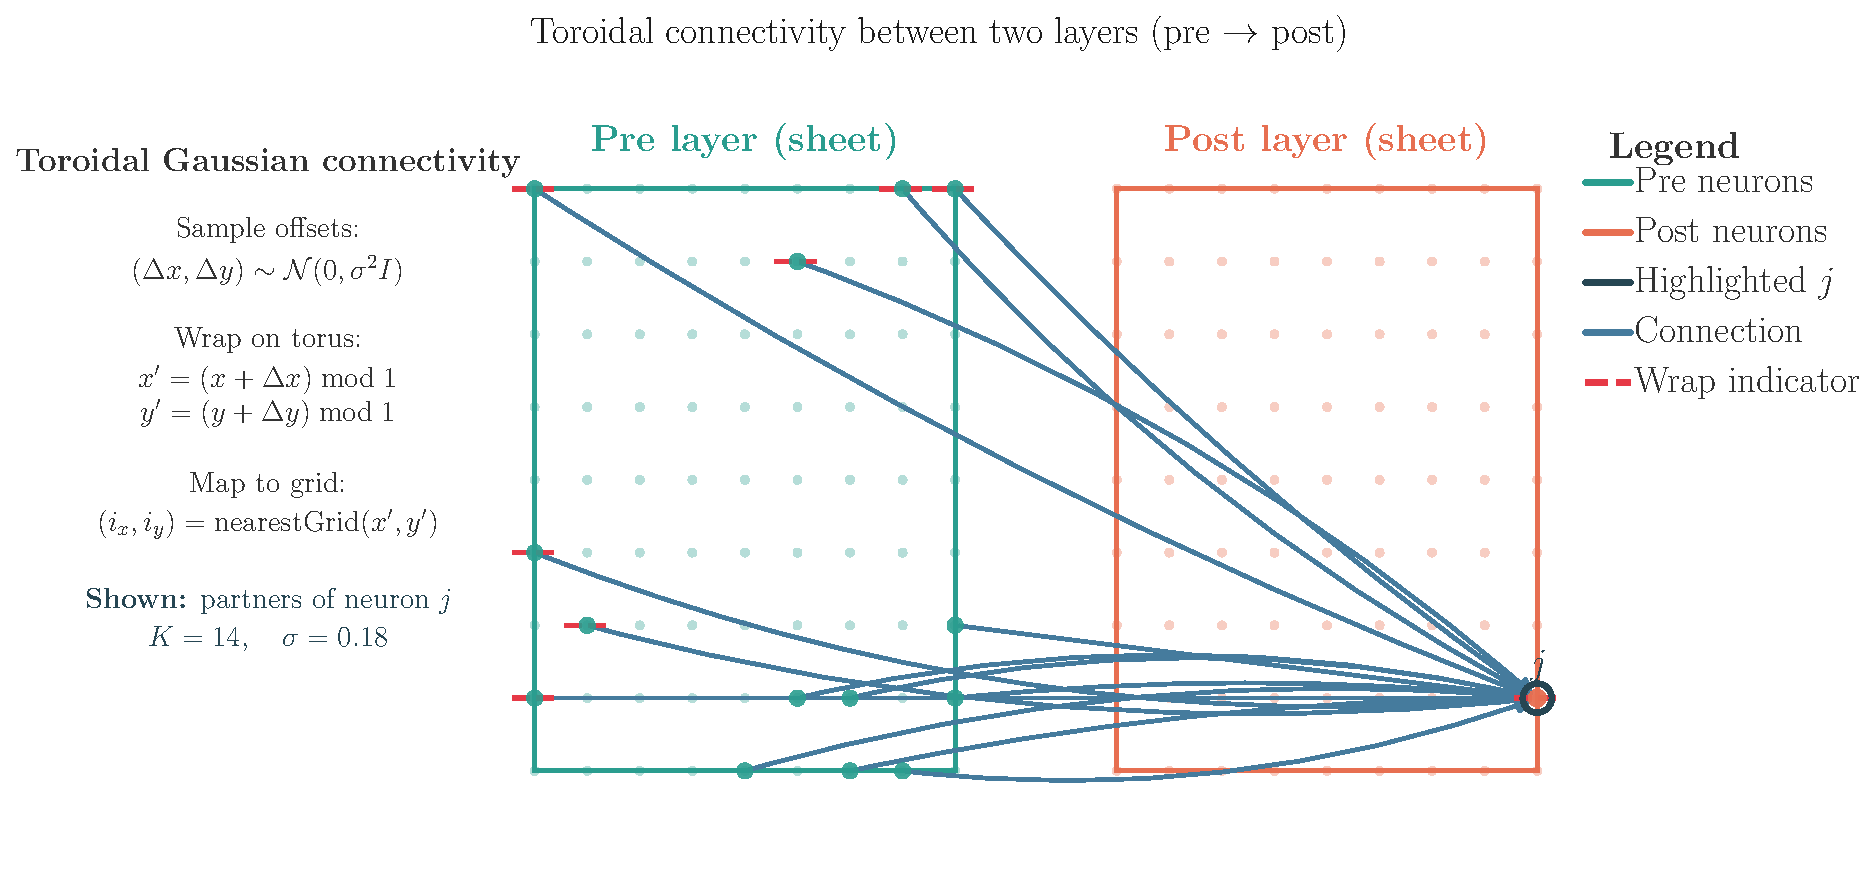
\includegraphics[width=1\linewidth]{images/toroidal_connectivity_two_layers.pdf}
    \caption[Toroidal Gaussian connectivity scheme]{
        \textbf{Toroidal Gaussian connectivity between the pre- and
        post-synaptic layers.}
        Each neuron $j$ in the post-synaptic layer (orange, right) receives
        input from $K$ pre-synaptic neurons (teal, left) sampled according
        to a 2-D Gaussian centred on the position of $j$ in the sheet.
        Offsets $(\Delta x, \Delta y)\sim\mathcal{N}(0,\sigma^2 I)$ are
        drawn in normalized coordinates $[0,1)^2$ and wrapped toroidally,
        so neurons near one border can connect to neurons near the opposite
        border; such wrap-around connections are indicated by dashed red
        markers.
        The sampled offset is then mapped to the nearest grid index,
        yielding a spatially structured but stochastic receptive field.
    }
    \label{fig:toroidal_connectivity}
\end{figure}

\clearpage
\subsection{Weight initialization}
\label{sec:weight-init}

Initial weights are drawn from a Gaussian whose mean and standard deviation
are scaled by the fan-in,
%
\begin{equation}
W_{ji} \sim \mathcal{N}\!\left( \mu, \, s^2 \right),
\qquad
\mu = \mathrm{sign}(i)\,\frac{c}{\sqrt{K}},
\qquad
s = \frac{\sigma_w}{\sqrt{K}},
\label{eq:weight_init}
\end{equation}
%
where $\mathrm{sign}(i) \in \{+1, -1\}$ is the Dale sign of the presynaptic
population. The $1/\sqrt{K}$ scaling makes the expected total synaptic drive
onto a neuron independent of its fan-in and of the layer width, keeping input
currents, and hence firing rates, in a stable operating range across
populations of different size and across depth, which prevents the saturation
or silencing that would otherwise impede the propagation of eligibility
traces. The mean magnitude $c$ is set asymmetrically for the two types:
excitatory connections use a small mean ($c_E = 0.1$), whereas inhibitory
connections use a substantially larger mean ($c_I = 3$). This asymmetry
restores the excitatory-inhibitory balance because the inhibitory population
is smaller, boosting the per-synapse inhibitory weight
ensures that the net inhibitory and excitatory drive onto a typical neuron are
comparable at initialization. The dispersion is common to both
($\sigma_w = 0.05$). Unconstrained readout and feedback connections, which
carry no Dale sign, are initialized with zero mean and a variance scaled by
the number of output units, $s = 1/\sqrt{N_{\text{out}}}$.

\subsection{A Weakened Dale's Law}
\label{sec:weakened_dale}

Dale's principle is imposed only at initialization. Every hidden neuron is assigned a
type, and through Equation~\ref{eq:weight_init} its outgoing weights take the
corresponding sign, so the network begins from a structured excitatory-inhibitory
configuration. During training, however, the sign constraint is not re-imposed, the updates are applied directly to the weights, with no projection back onto the
presynaptic sign and no sign-preserving regularizer or rewiring step active. Individual
synapses are therefore free to change sign over the course of learning.

This specific combination was arrived at empirically, and is consistent
with prior findings on training artificial networks under Dale's
principle. \citep{Song2016DaleEI} similarly report that simply
partitioning a recurrent network's units into excitatory and inhibitory
populations and enforcing the constraint throughout training impairs
learning relative to an unconstrained network, motivating frameworks that
relax or restructure the constraint.
More recently, \citep{Cornford2021DaleANN} address this
directly under the heading of ``learning to live with Dale's principle,''
showing that standard feedforward and convolutional networks can respect
the excitatory/inhibitory separation throughout training without
sacrificing performance, provided the architecture and initialization are
adapted accordingly. Two stricter alternatives were evaluated
here and found to be insufficient. initializing without any sign
structure, that is, treating excitatory and inhibitory neurons as
identical at the start of training, resulted in networks that failed to
learn entirely. Enforcing the sign constraint throughout training, by
clipping or rewiring, preserved the EI
structure but consistently hindered learning.

The weakened variant threads between these two failure modes. initializing under
Dale's law provides a well-structured excitatory-inhibitory balance at initialization, which stabilises the network dynamics and allows eligibility
traces to propagate effectively from the first steps of training. Releasing the
constraint afterwards gives the optimizer the freedom to move weights wherever the
learning signal requires, without being stalled by a hard sign boundary. The network
thus benefits from the structural properties of the EI initialization while remaining
unconstrained during the learning process itself.

\subsection{Feedback Connectivity}
\label{sec:feedback_connectivity}

Online e-prop requires that specific quantities reach each hidden synapse to drive
learning. The precise set of quantities depends on which variant of the algorithm is
used. We describe the three distinct feedback pathways involved and specify which are
required by each variant.

\paragraph{Forward readout.}
Each output head is a non-spiking leaky-integrator readout of its dedicated field
population (Section~\ref{sec:depth_ei}). Both the excitatory and inhibitory units of
the field project onto the head through dense, sign-unconstrained readout weights.
Because the readout is a linear, non-recurrent transformation of the field activity,
the gradient of the loss with respect to these weights is exact and is computed by
standard gradient descent; no approximation of the kind introduced by e-prop is
needed or applied here. The policy head integrates four such readouts (one per action)
and the value head a single one.

\paragraph{TD error broadcast.}
The value head computes the temporal-difference error
\begin{equation}
    \delta^t = R_{t+1} + \gamma V_{t+1} - V_t,
\end{equation}
and this scalar is broadcast, unchanged, to every population in the network (the core
excitatory and inhibitory units, both field populations, and the policy head). The
broadcast is implemented through unit-weight connections, so that
\begin{equation}
    \delta^t_j = \delta^t \quad \text{for every neuron } j.
\end{equation}
This pathway carries no per-neuron weights and requires no random projection. It is a
single neuromodulatory-like signal that is uniformly applied to the local credit traces. This pathway is present in both standard e-prop and
distributed e-prop.

\paragraph{Policy feedback connections.}
In standard e-prop, the policy head supplies a structured learning signal to the hidden
populations. The policy-gradient term $\pi^t_k - \mathbf{1}_{a_t = k}$ is projected
back onto each hidden neuron $j$ through a set of feedback weights $B^\pi$,
\begin{equation}
    L^{\pi,t}_j = \sum_k B^\pi_{kj} \left( \pi^t_k - \mathbf{1}_{a_t = k} \right).
\end{equation}
The feedback matrix $B^\pi$ can be instantiated in several ways, as a fixed random
projection (random e-prop), as a transpose copy of the forward readout weights
(symmetric e-prop), or as an adaptively learned matrix (adaptive e-prop). In all cases the role is to provide each neuron with a per-neuron approximation of the policy gradient.
This pathway is absent in distributed e-prop.

\paragraph{Value feedback connections.}
Analogously, the value head routes a per-neuron approximation of the value gradient
back to the hidden populations through a feedback matrix $B^V$,
\begin{equation}
    L^{V,t}_j = 
        B^V_j,
\end{equation}
where $B^V_j$ is the feedback weight from the value head to neuron $j$. As with the
policy feedback, $B^V$ can be symmetric, random, or adaptive. This signal allows
each neuron to approximate its individual contribution to the value estimate, and is
distinct from the TD error broadcast, whereas the broadcast delivers the scalar
$\delta^t$ with unit weights to gate all updates uniformly, the value feedback
delivers a per-neuron projection of the value gradient to shape how hidden neurons
adjust their contribution to $V_t$. This pathway is also absent in distributed e-prop.

\paragraph{Distributed routing connections.}
In the routed variants of distributed e-prop, each neuron's local,
perturbation-derived signal is not used in isolation but is additionally
propagated through the recurrent connectivity, so that each neuron receives a
contribution from the local signals of the neurons it connects to. Crucially,
in this implementation the routing weights are not a separate feedback matrix
but the recurrent weights $`W^{\mathrm{rec}}`$ themselves,
\begin{equation}
L^{\mathrm{rec},t}_j = \sum_k W^{\mathrm{rec}}_{jk}\, s_k^t,
\end{equation}
where $`s_i^t`$ is the local signal of neuron $`i`$. This makes the pathway
directly analogous to symmetric e-prop, in which the feedback weights are tied
to the forward weights, with the difference that here the routing reuses the
network's own recurrent connectivity,
and no dedicated feedback matrix is introduced. This pathway is present only in
the routed variants of distributed e-prop; it is absent in standard e-prop and
in the purely local, broadcast-only distributed variants.

\paragraph{Summary.}
The variants differ in precisely which feedback pathways are active. Standard
e-prop uses the TD error broadcast, the policy feedback connections, and the
value feedback connections, providing each neuron with structured, per-neuron
approximations of both the policy and value gradients. The broadcast-only
distributed variants use only the TD error broadcast, with each neuron relying
entirely on its own perturbation and eligibility traces to determine how its
incoming connections should be updated. The routed distributed variants
additionally reuse the recurrent connectivity $`W^{\mathrm{rec}}`$ as a
structured routing pathway for the local signal, occupying an intermediate
position, more structure than the broadcast alone, but without the dedicated,
non-recurrent feedback matrices of standard e-prop.

% ─────────────────────────────────────────────────────────────
\section{Implementation}
\label{sec:implementation}

This section describes the implementation contribution and how the learning rule and network are
realized in practice. The implementation choices follow directly
from the constraints established in Chapter~\ref{ch:sota}:
strict locality, online (no-replay) updates, and a continuing
task formulation with no internal state resets. Each design
decision is therefore made with the explicit goal of preserving
those properties on real hardware while keeping training
tractable.

The complete source code for all models, learning rules, and experiments is
openly available at \url{https://github.com/Nordest27/ml_genn}.
% ─────────────────────────────────────────────────────────────
\subsection{Simulation Substrate}
\label{subsec:framework}

The network is implemented on top of GeNN \citep{Yavuz2016GeNN} via its high-level Python interface
\texttt{ml\_genn}, with a custom compiler derived from
\texttt{EPropCompiler} to support the modifications introduced
in this work (TD($\lambda$) integration, arbitrary feedback connections, distributed per-synapse
perturbation, \ldots).

GeNN is a GPU-accelerated, just-in-time-compiled spiking neural
network simulator that generates CUDA kernels from
user-specified neuron, synapse, and weight-update models. Three
properties of this substrate are essential to the present work:

\textbf{Event-driven semantics.}
Spiking activity is sparse, most neurons are silent at any
given timestep, and updates that depend on presynaptic
spikes are only triggered
on emission. This makes the inference per-step cost of the network
scale with mean firing rate, and not with neuron count,
which is the regime under which biological networks
operate and the regime in which neuromorphic hardware is
designed to excel.

\textbf{Per-synapse state at full parallelism.}
The plasticity rule requires several variables to be
maintained \emph{per synapse} (the filtered eligibility
trace $\bar e_{ij}$, the local noise trace, the
eligibility-trace) gated reward traces, and, in the distributed
variant, the per-synapse log-variance $\log\sigma_{ij}$.
GeNN stores these on-device and updates them in a single
fused CUDA kernel per synapse population, which makes the
per-synapse state cost manageable even for sparse
connectivities on the order of $10^{5}$ to $10^{6}$ synapses.

\textbf{Alignment with the target deployment
regime.}
Because the same model definition is used for both
simulation and (in principle) deployment on
spike-driven accelerators, the implementation acts as a
faithful prototype of how the rule would run on
neuromorphic substrates such as Loihi \citep{Davies2018Loihi}, SpiNNaker \citep{Painkras2013SpiNNaker}, or similar event-based platforms. Every operation we use is
expressible as a local per-synapse update, where all feedback information comes from connections that also live in the network.

The choice of GeNN is therefore a structural commitment, the algorithmic constraints of the
learning rule (locality, online updates, no episodic resets)
and the architectural constraints of the substrate (event-driven
execution, per-synapse state, no global backward pass) are
selected to match each other.

% ─────────────────────────────────────────────────────────────
\subsection{Continuing-Task Interaction Stream}
\label{subsec:training_loop}

The training procedure departs from the standard episodic RL
paradigm in two related ways. First, the agent operates on a
\emph{continuing} interaction stream, although the environment emits an ending signal at the end of
each game, this signal is used only to reset the
\emph{environment state}, not the \emph{network state}. The
network's membrane potentials, adaptive thresholds, eligibility
traces and perturbation traces, all persist
across game boundaries. From the network's perspective there is
no terminal state, only a continuous sequence of locally good
and locally bad transitions.

A single environment step is mapped to $K$ consecutive
simulation timesteps. The active observation is converted to a
spike train by independent Bernoulli sampling, concretely, each input pixel
intensity defines a per-timestep firing probability, and the
spikes are queued into the GPU using those probabilities. The
action is sampled at the first timestep of the window from the
readout of the policy head.

For selecting categorical actions, the logits are read from a decaying integrator readout, normalized by softmax, and then 
sampled. The corresponding policy-gradient vector
$\nabla_{z} \log \pi(a \mid s) = (\pi - y)$ is written into
the policy head living in the GPU. Reward is propagated to the value head at each timestep through a decaying trace 
of the environment raw reward; the TD residual is computed
in the GPU as
$\delta_t = \gamma V_{t+1} + R_{t+1} - V_{t}$
and broadcast as a scalar feedback to all
synapses via dedicated connections, with weight equal to $1.0$.

\noindent
After the action is committed, the remaining $K-1$ timesteps of
the window propagate the spike-coded observation through the
network. At the end of every window the gradient update is executed,
applying the accumulated $\Delta g_{ij}$ to each weight via the Adam
optimizer. \emph{No replay buffer is used and no backward pass
is performed at any point.} The update is purely an online
read-modify-write of per-synapse state.

Because every per-synapse computation depends only on the
state of its endpoints and on broadcast scalars, the
plasticity rule maps to a single fused kernel that updates
all synapses in a population in parallel. There is no
serial dependency between synapses, no global accumulator
beyond the broadcast scalars, and no backward sweep over
the network graph. This is what allows the rule to scale
to networks with $\sim$1{,}900 hidden neurons and millions 
of synapses while running online (one
gradient update per environment step, no batching across
trajectories).

% ─────────────────────────────────────────────────────────────

\begin{table}[h!]
\centering
\small
\begin{tabular}{@{}l l l@{}}
\toprule
\textbf{Group} & \textbf{Symbol / name} & \textbf{Value} \\
\midrule
\multicolumn{3}{l}{\textit{Neuron model (ALIF, all hidden populations)}} \\
& Threshold $v_{\mathrm{th}}$ & 0.61 \\
& Membrane time constant $\tau_{\mathrm{mem}}$ & 10 ms \\
& Refractory period $\tau_{\mathrm{refrac}}$ & 3 ms \\
& Adaptation time constant $\tau_{\mathrm{adapt}}$ & 300 ms \\
& Adaptation strength $\beta$ & 0.0174 \\
& Surrogate gradient sharpness & 0.3 \\
\midrule
\multicolumn{3}{l}{\textit{Network architecture}} \\
& Input population shape & Task Dependant \\
& Hidden E shape & $20 \times 20 \times 3$ (1200 neurons) \\
& Hidden I shape / Policy / value field shape  & $15 \times 15 \times 3$ (675 neurons) \\
& Output heads (policy / value) & (4 or 7) / 1 \\
\midrule
\multicolumn{3}{l}{\textit{Connectivity}} \\
& Connectivity type & toroidal Gaussian \\
& $\sigma$ (input $\to$ hidden) & 0.1 \\
& $\sigma$ (hidden $\to$ hidden, hidden $\to$ field) & 0.05 \\
& Target fan-in & 100 \\
& Dale's law sign & enforced per neuron (init) \\
\midrule
\multicolumn{3}{l}{\textit{Learning}} \\
& Optimizer & Adam \\
& Learning rate $\eta$ & Task Dependant\\
& Batch size & 1 \\
& Action window $K$ & 30 timesteps \\
& Discount $\gamma$ (per env. step) & 0.5 \\
& Trace decay $\lambda$ (per env. step) & Task Dependant \\
& Reward trace decay $\kappa$ (per env. step) & Task Dependant \\
& Firing-rate regularization $c_{\mathrm{reg}}$ & $10^{-4}$ \\
& Target firing rate $F^{*}$ & 10 Hz \\
\midrule
\multicolumn{3}{l}{\textit{Distributed perturbation (where applicable)}} \\
& $(weight\ variant)\log \sigma_{j}$ & $-5$ \\
& $(weight\ variant)\log \sigma_{ji}$ & $-5$ \\
& $(neuron\ variant)\log \sigma_{j}$ & $-4.61$ \\
\bottomrule
\end{tabular}
\caption{Network and learning hyperparameters. Values match
those used in the experiments of
Chapter~\ref{ch:results}. Time-extended quantities are
reported per environment step ($K=30$ simulation timesteps);
their per-timestep values are obtained by raising to the
$1/K$ power.}
\label{tab:hyperparams}
\end{table}

% -----------------------------------------------------------------
\subsection{An Idealised Gradient-Based Ceiling: PPO}
\label{subsec:ppo_ceiling}

The learning rules studied in this thesis are deliberately constrained, as they
are strictly local, update online without a replay buffer, and never perform
a backward pass. These constraints are what make the rules plausible
candidates for neuromorphic hardware and fit for tasks that are inherently non-episodic. However, they also make it hard to know, for
a given task and network size, how much performance is being given up in
exchange for that plausibility. To provide a reference point, we additionally
train a conventional, unconstrained agent with Proximal Policy Optimization
(PPO)~\citep{schulman2017ppo} and treat its performance as an approximate
\emph{ceiling}, the level a strong gradient-based optimizer reaches on the
same task, against which the local rules can be evaluated. This baseline was run
as a lightweight comparison, and the
details below are reported only to make the experiment of
Section~\ref{sec:ppo_ceiling} interpretable.

It is important to stress that this baseline is \emph{not} a spiking network
and is subject to none of the constraints above. It is a standard
(non-spiking) convolutional actor-critic with a shared three-layer
convolutional trunk feeding separate policy and value heads, trained by full
backpropagation with the clipped PPO surrogate objective, generalized
advantage estimation (GAE)~\citep{schulman2016gae}, and several optimization
epochs over each collected roll-out using the Adam optimizer. Every one of
these ingredients, the dense gradients routed by backpropagation, a stored
roll-out replayed across multiple epochs and a single global objective
optimized end-to-end, is what the local rules of this chapter avoid. The PPO agent should therefore be read as an upper reference for what
the task affords a capable optimizer, not as a like-for-like competitor to
the spiking models.

The one design choice we deliberately mirror from the spiking setup is the
\emph{continuing} task formulation introduced in
Section~\ref{subsec:training_loop}. Recall that the spiking agent never sees
a terminal state, the environment's ending signal resets the
\emph{environment} but not the \emph{network}, so value estimates and credit
flow across game boundaries as if the interaction were one uninterrupted
stream. We expose the same distinction in PPO through a single switch in the
advantage computation. Standard GAE multiplies both the value bootstrap and
the recursive advantage term by a mask $(1 - d_t)$ at every step, where $d_t$
is the \emph{episode ended} flag; this mask is exactly what stops advantage from
leaking across an episode boundary, and is what makes PPO optimize the
\emph{discounted episodic return}. Disabling the mask (holding the factor at
$1$ even when $d_t = 1$) lets the bootstrap and the advantage recursion run
straight through resets, so the agent no longer optimizes return-per-episode
but the reward accumulated over the uninterrupted stream, i.e. a
\emph{reward rate}. We refer to these two configurations as the
\emph{episodic-objective} and \emph{continuing-objective} variants of PPO,
and use the contrast between them in Section~\ref{sec:ppo_ceiling} both to
bound achievable performance on Snake $5\times5$ and to make explicit the
distinction between the two performance metrics reported throughout
Chapter~\ref{ch:results}.
\clearpage

 \subsection{Network and Learning Configuration}
\label{subsec:hyperparameters}

Table~\ref{tab:hyperparams} lists the values used throughout
the experiments reported in Chapter~\ref{ch:results}. Time
constants are given in milliseconds with $\Delta t = 1$ ms.
Discount factors and trace decays are listed at the
\emph{per-environment-step} resolution, their per-timestep
values are obtained as $x^{1/K}$ with $K=30$, so that the
effective decay over one action window matches the value
stated here.

%─────────────────────────────────────────────────────────────
\subsection{Experimental Environments}

Three environments are used to evaluate the learning framework, each designed to stress
a distinct combination of capabilities and to provide interpretable evidence about different
aspects of the algorithm's behavior.


\begin{figure}[H]
    \centering
    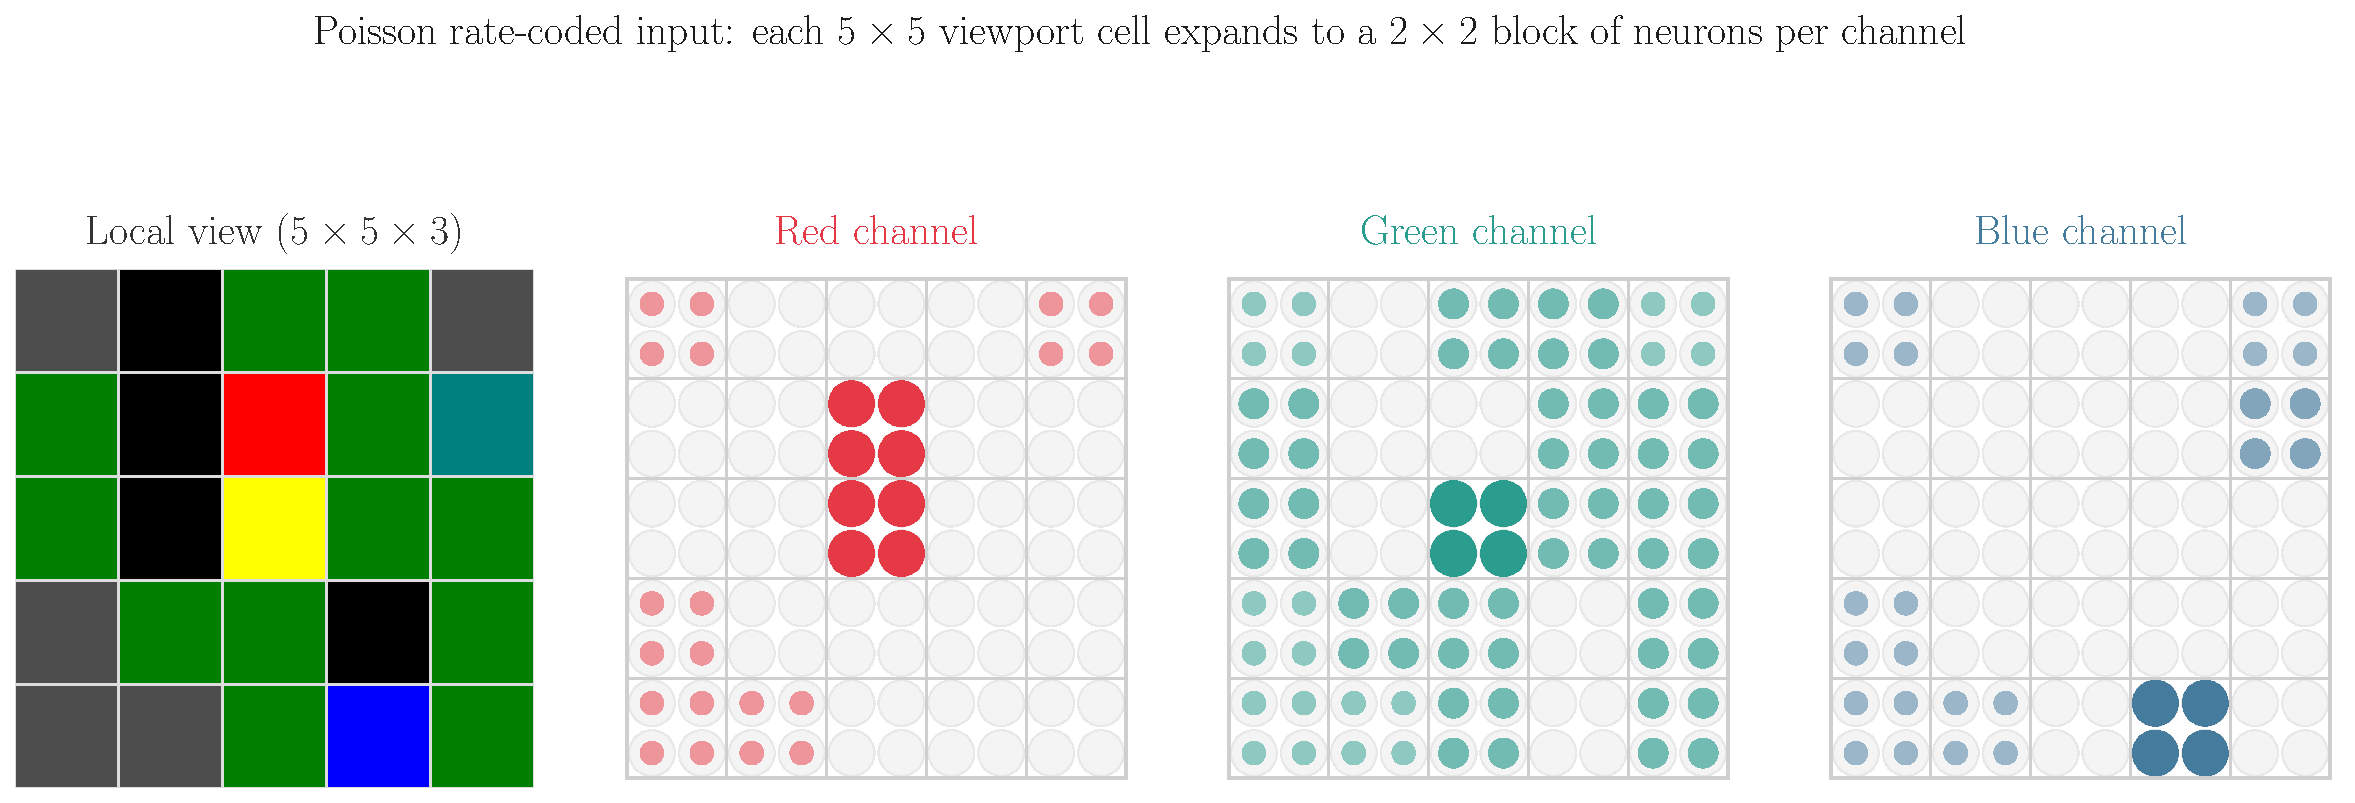
\includegraphics[width=1.0\textwidth]{images/poisson_input_encoding.pdf}
    \caption[Poisson rate-coded input encoding]{Poisson rate-coded encoding of the agent's observation. The $5\times5$ 
    view (left) is upscaled so that each cell becomes a $2\times2$ block of input neurons 
    in each of the three channels. Each neuron fires as a sequence of Bernoulli trials whose 
    probability is proportional to the corresponding channel intensity, up to a maximum of 
    $p_{max}$. Circle size and opacity are proportional to the firing probability.}
    \label{fig:poisson_input}
\end{figure}


\subsubsection{Agent's Input}
Before describing the individual tasks, we first introduce the common way in which 
all agents perceive their environment. Each agent observes a small grid-shaped view of the environment, encoded as a set of spike 
trains that the spiking network can process directly.

Concretely, the observation is a grid with three channels, which encode the different 
elements of the environment through distinct color intensities. This compact image is then upscaled 
so that each cell of the view is represented by a small $U \times U$ block of input neurons per 
channel, where $U$ is the upsampling scale, and every neuron is converted into a Poisson spike train whose firing probability is 
proportional to the corresponding channel intensity, up to a maximum of $p_{max}$. In this way, 
a brighter input drives its neuron to fire more often, while an empty cell remains silent, and 
the continuous observation is turned into the temporal, event-based signal that the network 
consumes at each step.

Figure~\ref{fig:poisson_input} illustrates this encoding for a representative observation. 
The left panel shows the view as the agent receives it, and the three panels on the right 
show the resulting per-channel grids of input neurons, where the size and opacity of each circle 
reflect how strongly that neuron fires. This same scheme is used across all the environments 
considered in this chapter; only the meaning of the elements in the scene changes from one task 
to another.

\subsubsection{Environment 1: Snake} 
\begin{figure}[H]
    \centering
    
\includegraphics[width=0.3\linewidth]{snake.png}
    \caption[The Snake environment]{The Snake environment, rendered as an RGB image: the green cells trace the
    snake's body, the red cell marks the food, and the grey border denotes the
    walls. The agent perceives only a $5\times5$ window centred on the head.}
    \label{fig:placeholder}
\end{figure}

The Snake environment places the agent in a grid world in which it must navigate a
growing body to collect food pellets without colliding with itself or the walls. The agent
receives a local pixel observation centred on the head, covering a fixed window of
$5 \times 5$ cells rendered as an RGB image.

This environment probes several distinct capabilities simultaneously. At the level of
reactive control, the agent must avoid immediate self-collision, which requires integrating
the current direction of motion with the local layout of the body. Crucially, reversing
direction is physically prevented, so the agent must commit to actions whose consequences
unfold over multiple steps and cannot be corrected immediately. This tests whether the
learning rule can shape a policy that avoids locally attractive but globally harmful actions,
and whether the eligibility traces retain sufficient signal to assign credit across the
relevant horizon.

The reward signal is relatively sparse, a positive reward is delivered only upon eating a pellet,
and a strong negative reward upon death, with no intermediate shaping. Whether the
algorithm can propagate this sparse signal back across the steps that preceded it is
therefore directly observable from the agent's ability to collect food consistently.

\subsubsection{Environment 2: Pac-Man}
\begin{figure}[H]
    \centering
    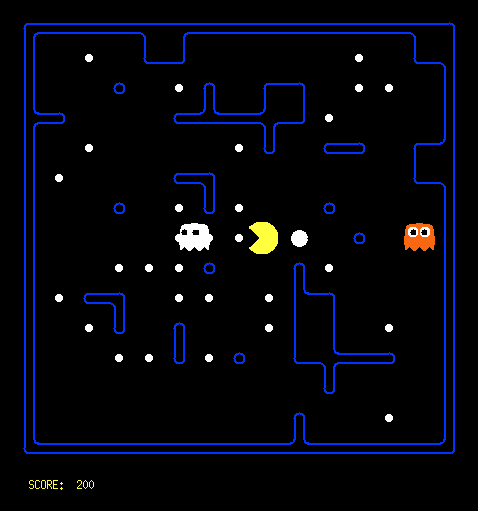
\includegraphics[width=0.35\linewidth]{pac-man.png}
    \caption[The Pac-Man environment]{The Pac-Man environment. The agent (yellow) collects pellets and power
    capsules while avoiding ghosts; eating a capsule briefly frightens the ghosts (white),
    making them edible before they return to pursuing (orange). Walls restrict the legal
    moves differently at each position, and rewards span several magnitudes dependant on pellets,
    frightened-ghost captures, and the penalty for being caught.}
    \label{fig:placeholder}
\end{figure}
The Pac-Man environment places the agent in a maze populated by food pellets, power
capsules, and ghost enemies. The agent receives a local pixel observation centred on its
current position and must navigate the maze to collect food while avoiding or, when
powered up, pursuing ghosts.

Unlike the preceding environment, Pac-Man combines several sources of reward
structure simultaneously. Positive rewards arrive at irregular intervals as pellets are
collected, large positive rewards are available for eating frightened ghosts, and a strong
negative reward follows capture by an active ghost. The mix of timescales (dense local
rewards from pellet collection interleaved with rare but high-magnitude events from ghost
interactions) could allows us to evaluate whether the learning rule can simultaneously support
short-horizon reactive behavior and longer-horizon strategic planning within the same
task.

A distinctive feature of this environment is the prevalence of invalid actions. At any
given position, walls constrain the agent to a strict subset of the four cardinal directions,
and the legal set changes at every step as the agent moves through the maze. This
requires the policy to handle a persistent mismatch between the network's fixed
four-dimensional output and the variable-cardinality legal set, and provides a direct test
of how the algorithm manages probability mass assigned to unavailable actions. 

The ghost dynamics introduce a non-stationary element, ghost behavior switches between
chasing and retreating depending on the capsule state, and the agent must learn to
condition its behavior on this mode, which is only partially observable from the local
viewport. This tests the network's ability to use its recurrent state to disambiguate
situations that appear similar from a single-step observation, providing evidence about
the practical utility of the recurrent dynamics for contextual adaptation.

The environment is the classic implementation from the UC Berkeley
CS188 Pac-Man AI projects~\citep{denero2010pacman},\footnote{\url{https://ai.berkeley.edu}}
which we accessed through a Python~3.7 port provided by the thesis supervisor.
We extended this environment with procedurally generated layouts and a
continuing-task formulation without episodic resets.

\subsection{The Randomized Layouts Problem}

In this problem, the agent is placed in a $15 \times 15$ maze enclosed by walls and partially filled with interior obstacles that divide the space into a connected network of corridors. The maze is fully connected, so every open cell (and therefore every item and ghost) is reachable from any starting position. Scattered throughout the corridors are food pellets, two power pellets, and two ghosts, and the agent controls Pac-Man, whose objective is to clear the maze of food while avoiding the ghosts.

Crucially, the maze and the placement of all entities differ in every episode. The agent never sees the same configuration twice: walls, food, power pellets, ghosts, and its own starting position are all arranged differently each time. As a result, the agent cannot rely on a memorized map of the environment. It must instead learn a policy that operates entirely from its current local observation, generalizing across the wall configurations and entity placements it encounters.

At each step, the agent perceives a local window centered on Pac-Man and selects one of four movement directions. The reward reflects the outcome of each action, the agent receives a reward of $+1.0$ for eating a food pellet or a power pellet, $+2.0$ for catching a ghost that has been made vulnerable, and $-2.0$ when it is caught by an active ghost. Ordinary movement through empty corridors yields no reward, so the agent is neither rewarded nor penalized for exploration in itself, but exploration is rewarded anyway through the pellets. This scheme drives the agent to consume food and exploit vulnerable ghosts while avoiding fatal encounters.

The agent does not perceive the maze in its entirety, at each step it only observes a small $5 \times 5$ window centered on Pac-Man, leaving the rest of the maze hidden. It must therefore act under partial observability, inferring how to move toward food and away from ghosts from a narrow local view. This restricted window is a double-edged design choice. On the one hand, it limits the information available to the agent, hiding distant food and approaching ghosts and forcing it to act on incomplete knowledge. On the other hand, because the window is always centered on Pac-Man, the observation is inherently translation-invariant and low-dimensional meaning that the same local pattern always maps to the same relative situation regardless of where Pac-Man is in the maze. This compactness and consistency greatly reduce the size of the input space the network must learn to interpret, which accelerates learning and makes the policy easier to generalize across layouts.

The balance between partial observability and learning velocity is also shaped by the nature of the model itself. Because we employ SRNNs, partial observability is far less limiting than it would be for a purely feedforward architecture. The recurrent connectivity endows the network with an internal memory, information from previous observations persists in the network state and is integrated over time, allowing the agent to build an implicit, evolving representation of its surroundings as it moves. In effect, the network can compensate for the narrowness of any single observation by accumulating evidence across successive steps, so the $5 \times 5$ window restricts the instantaneous input far more than it restricts the information actually available to the policy.

Finally, although the constantly changing layout would in principle make this task harder than solving a single fixed maze, in the context we work in this variability is in fact necessary. The algorithms we employ are prone to action overcommitment, whereby an initial bias toward particular actions or strategies is quickly reinforced and ends up nullifying further learning. By continually varying the layout, we prevent such premature convergence and force the agent to keep learning a general, reactive strategy for collecting food and evading ghosts rather than a solution tailored to any single configuration. For this environment we used per-episode updates, as per-action updates were found to reliably collapse training.

\subsubsection{Environment 3: Connect Four}
\begin{figure}[H]
    \centering
    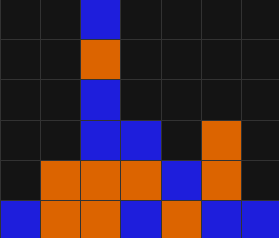
\includegraphics[width=0.35\linewidth]{connect-4.png}
    \caption[The Connect Four environment]{The Connect Four environment. Tokens are dropped into the columns of a
    $6\times7$ grid, with the agent's and opponent's pieces shown in blue and orange, and
    the goal is to align four in a row before the opponent. The full board is rendered as
    an RGB image at every turn, and rewards are sparse: $+1$ for a win, $-1$ for a loss,
    and $0$ otherwise.}
    \label{fig:placeholder}
\end{figure}
The Connect Four environment presents the agent with a two-player, turn-based board
game in which pieces are dropped into columns of a $6 \times 7$ grid and the objective
is to form a horizontal, vertical, or diagonal line of four consecutive pieces before the
opponent does. The full board state is rendered as a pixel image and provided to the
agent at each turn.

The reward structure is maximally sparse: a reward of $+1$ is delivered upon winning,
$-1$ upon losing, and $0$ at every intermediate step. The consequence of any individual
move may only become apparent several turns later when a winning or losing configuration
is completed. This makes the environment a direct test of long-horizon action credit
assignment, because the learning rule must attribute the terminal outcome back to the sequence
of placements that caused it, with no intermediate signal to guide this attribution.

The opponent is configured as a heuristic agent that blocks the agent's immediate winning
moves when it detects them, and wins in one-move if it detects the win, but does not plan beyond a single move ahead and can
therefore miss multi-step threats. The agent must learn to build attacking and defensive
patterns that exploit this limited lookahead, which requires recognizing recurring board
configurations and understanding which structural features carry strategic significance.
This makes pattern recognition over a structured spatial input a central demand of the
task, and allows us to evaluate whether the network's spatial organization supports the
development of such representations.

The combination of maximally sparse rewards, a reactive but imperfect opponent, and
spatially structured winning conditions makes Connect Four a clean testbed for isolating
the credit assignment and pattern recognition capabilities of the learning rule, with
outcomes that are directly interpretable in terms of win, loss, and draw rates.

Taken together, the three environments are complementary. Snake provides a controlled setting for studying sparse credit assignment,
reactive commitment, and scalable working memory, Pac-Man introduces a richer and more mixed setting in which dense
and sparse rewards coexist, illegal actions are pervasive, and the relevant context is
partially observable, allowing us to evaluate the algorithm's behavior when multiple
demands are present simultaneously and Connect Four isolates long-horizon
credit assignment and spatial pattern recognition under maximally sparse rewards and a
structured opponent. For this environment we used per-episode updates, as per-action updates were found to reliably collapse training.

\chapter{Experimentation and Evaluation}
\label{ch:results}

This chapter presents the experimental evaluation of the learning rules and
network architecture developed in Chapter~\ref{ch:method}. The central
empirical question is whether distributed e-prop, a learning rule that relies
solely on a globally broadcast scalar signal and local perturbation traces,
can learn effectively in challenging reinforcement learning tasks, and under
what conditions it becomes a limitation relative to more structured
feedback-based approaches. Beyond raw task performance, we also examine how
each learning rule affects the internal spiking dynamics of the network,
including membrane voltage and firing frequency, as these reveal whether a
given rule drives the network into a healthy operating regime or toward
pathological activity patterns that undermine learning.

The chapter is organized as follows. We begin by describing how the
experimental figures should be read and what each reported metric captures, followed by a brief description of the
naming conventions used for the different learning rule variants.
The chapter compares distributed e-prop against adaptive
e-prop across tasks of increasing complexity, examining the effect of network
depth, and the sensitivity of each rule to the
credit assignment horizon controlled by $\lambda$.

\section{Reading the Figures}
\label{sec:reading-figures}
Throughout this chapter, the results of each experiment are summarized in a single multi-panel 
figure. The quantitative figures follow the same pattern, the horizontal axis always denotes the training 
episode (typically up to $10{,}000$ episodes), and each panel tracks the evolution of one quantity 
over the course of training. Depending on the experiment, the individual curves correspond either 
to different credit-assignment variants (identified in the legend) or to a sweep over a particular hyperparameter, in which case the runs are differentiated either by a color gradient or a transparency gradient. Shaded bands for multi-seed runs represent the variability observed 
across repeated runs, and they show the variability for the single-run results. The solid line denotes the mean. Because the raw per-episode signals 
are noisy, the curves are smoothed with a running average so that the underlying trends remain 
legible.

Not every experiment in this chapter is repeated across multiple seeds. Several
of the comparisons that follow, report a single run per configuration, whereas the primary variant
comparisons on Snake and Pac-Man average over five independent runs with
the shaded bands described above. Because these two cases carry different
evidential weight, we read them in two correspondingly different ways, set out
explicitly here so that the claims made later in the chapter can be judged
against the evidence that actually supports them.

When a hyperparameter is swept, the individual curves are not read as isolated
point estimates but as samples of a single underlying response. If run-to-run
variability were large relative to the effect being swept, a one-run-per-value
sweep would appear jagged and incoherent; the fact that our sweeps are instead structured is itself evidence that the per-run noise is small compared with the trend.
Adjacent settings therefore act as approximate replicates of one another, since
each differs in both seed and hyperparameter, and their mutual consistency
constrains both at once. We treat such a coherent pattern as support for a
\emph{relational} claim, an ordering between variants, or the direction and
shape of a hyperparameter's effect. This reading is strengthened when the
observed trend agrees with the predicted mechanisms.

A single run is treated as a demonstration that a given behavior is
\emph{reachable}, not as an estimate of how typical it is. Establishing that a
phenomenon can occur requires only one instance, and for such existence claims
the number of repetitions is not the relevant measure. A single run in which
removing the pseudo-derivative $\psi_j^t$ diverges the membrane voltage, or in
which a large $\lambda$ collapses the network into near-silence, suffices to
establish that this outcome lies within the rule's behavioral repertoire under
the stated conditions. Single runs can also reinforce one another, when several
independent single-run experiments point the same way, and especially when they
agree with a behavior already observed consistently elsewhere in the chapter,
their convergence supports a qualitative claim that no one of them could carry
alone. What a single run cannot support \emph{on its own} is a comparative ranking,
which is inherently relational and is established only through the sweeps and
multi-seed comparisons above, or through the convergence of several mutually
consistent runs of the kind just described.

\subsection{Metrics}
Each figure reports the same six metrics, which together capture complementary aspects of the 
agent's behavior. The first two describe \emph{task performance}, the third describes the 
\emph{quality of value estimation}, and the last three describe the \emph{internal spiking 
dynamics} of the network:

\paragraph{Episode Reward.} The total reward accumulated by the agent over a complete 
episode. This is the most direct and interpretable measure of task performance as higher values 
indicate that the agent is collecting more reward (eating food, capturing an enemy, 
surviving longer, \ldots) before the episode ends. It should be noted, however, that because we operate 
in a continuous, no-reset configuration, the per-episode reward is not strictly the quantity 
being optimized; we report it primarily because it is intuitive and easy to relate to the 
agent's observable behavior.
    
\paragraph{Reward Rate.} The reward obtained per unit of time, that is, the accumulated reward 
normalized by the number of steps taken. The 
interaction is an uninterrupted stream in which states are merely more or less favorable, so the reward rate is arguably a more faithful reflection of what the agent is 
actually trying to maximize, since it does not depend on artificial episode boundaries. In 
practice we expect the two metrics to be strongly correlated, over episodes of comparable length, 
a higher total reward almost necessarily implies a higher reward per step, so the two largely move 
together and tend to tell the same story. They can nonetheless diverge, for instance when an 
agent accumulates more reward simply by surviving longer at the cost of acting less efficiently, and 
it is precisely these cases that make showing both informative. Since it is not clear that the 
agent fully optimizes the reward rate in practice, presenting the two side by side lets us see 
both how much reward is gathered and how efficiently it is obtained, without committing to a 
single notion of success.

\paragraph{TD Error (mean absolute value).} The average magnitude of the temporal-difference 
error, i.e. the discrepancy between the predicted value and the bootstrapped target at each step. 
In practice, these curves are difficult to draw firm conclusions from: a low TD error does not by 
itself guarantee a good policy, and the absolute values are hard to compare meaningfully across 
variants. At most, a TD error that grows or fluctuates wildly over training can be read as a sign 
of instability in value estimation, though even that interpretation is tentative. It is precisely 
this limited interpretability that motivates the qualitative value-trace results introduced later 
in this chapter, which offer a far clearer picture of whether the critic has learned anything useful.

\paragraph{Voltage.} The average membrane potential of the hidden neurons. This quantity 
shows the activity regime in which the neurons operate. High voltages are not desirable, as 
they produce pathological firing dynamics and nullify the possible learning of the affected 
neurons.
    
\paragraph{Voltage Loss.} A measure of how far the membrane potential deviates from the 
firing threshold, computed as the absolute value of the positive part of the 
voltage minus the threshold in both directions (i.e. 
penalizing the potential for exceeding the threshold from above or below). It is used 
internally as a regulatory signal that keeps neuron activity within a healthy operating range, 
and a rising voltage loss therefore indicates increasingly extreme membrane dynamics.

\paragraph{Frequency (Hz).} The average firing rate of the network, expressed in hertz. This 
metric is informative about whether the spiking population has settled into a healthy operating 
regime. Both extremes are undesirable and signal pathological dynamics, excessively high 
frequencies indicate runaway, saturated activity in which the neurons fire almost continuously and 
carry little information, while excessively low frequencies indicate a network that is largely 
silent and therefore unable to propagate or learn useful signals. A stable, intermediate firing 
rate is generally preferable, both for the health of the dynamics and for the energy efficiency 
of the solution.

Taken together, these metrics allow us to look beyond raw performance and examine \emph{how} each 
variant arrives at its policy. Two configurations may reach a similar episode reward yet differ 
substantially in the stability of their value estimates or in the regularity of their spiking 
activity, and these are the differences that motivate the comparisons presented in the 
remainder of the chapter.

\section{Qualitative Results: Value and Policy Traces}
\label{sec:value-traces}

Beyond the aggregate learning curves discussed above, we also include a set of \emph{qualitative} 
figures that look inside a single episode. These 
value-trace charts are intended to build intuition about \emph{what the trained agent has actually 
learned}, by showing how its internal predictions evolve step by step as it interacts with the 
environment.

Each value-trace figure follows one representative episode along the horizontal time axis, with one 
data point per environment step, and overlays the quantities the agent produces at every step. The 
central quantity is the \textbf{value estimate}: the output of the critic, which at each step 
predicts the expected (discounted) future reward from the current situation. Alongside it we plot 
the \textbf{reward trace}, an exponentially decaying accumulation of the rewards the agent receives, 
which serves as a smoothed reference signal of what is actually happening in the episode. Where 
relevant, we also show the \textbf{action probabilities} produced by the policy head, which reveal 
how confident or exploratory the agent is when choosing among the available actions.

The interpretation of these charts is qualitative. A well-trained critic should produce a value 
estimate that is predictive, it should rise in anticipation of 
upcoming reward and fall ahead of unfavorable outcomes. 
In other words, we expect the value curve to lead, and broadly track, the reward 
trace, and we dont want it lagging behind of the rewards or remaining flat and uninformative. 
The action probabilities, in turn, let us see whether the policy commits decisively 
to sensible moves at critical moments 
while retaining enough stochasticity to keep exploring otherwise.

These traces complement the quantitative metrics: whereas the aggregate curves tell us \emph{whether} 
and \emph{how stably} an agent learns, the value traces illustrate \emph{how} a learned policy and 
its critic behave moment to moment, offering a more interpretable picture of the agent's decision 
making that the averaged statistics alone cannot convey.

\section{Naming of Learning Rule Variants}
\label{sec:variant-naming}

Throughout this chapter, the figures compare several variants of the learning
rules developed in Chapter~\ref{ch:method}. Because the legend names used
in the plots are necessarily terse, Table~\ref{tab:variant-naming} provides a
key mapping each name to the specific algorithmic choice it refers to, together
with the section in which it was derived. This table is intended as a reference
point for the remainder of the chapter, so that a reader encountering, for
instance, \emph{weight dist ind noise} in a legend can immediately
identify which update rule from Section~\ref{sec:distributed_eprop} is being
evaluated.

% Requires \usepackage{tabularx} in the preamble — add it if not already present

\begin{table}[H]
    \centering
    \begin{tabularx}{\textwidth}{l X}
        \toprule
        \textbf{Legend name} & \textbf{Algorithm} \\
        \midrule
        \emph{baseline} & 
            Static recurrent and input weights, only the output weights are trained \\[4pt]
        \emph{symmetric} &
            Standard reward-based e-prop with symmetric feedback weights
            $W_{kj}$ (Section~\ref{sec:e-prop}) \\[4pt]
        \emph{adaptive} &
            Standard reward-based e-prop with adaptive, fixed feedback weights
            $B$ (Section~\ref{sec:e-prop}) \\[4pt]
        \emph{node dist} &
            Distributed e-prop, neuron perturbation variant: shared membrane
            noise $\varepsilon^t_j$ per neuron, no structured routing
            (Section~\ref{sec:distributed_eprop}) \\[4pt]
        \emph{node dist prop} &
            Neuron perturbation variant with structured routing of the local
            policy signal $L^t_j$ through the recurrent weights
            (Section~\ref{sec:distributed_eprop}) \\[4pt]
        \emph{weight dist} &
            Distributed e-prop, synaptic perturbation, shared-postsynaptic-noise
            variant with per-synapse scaling
            (Section~\ref{sec:distributed_eprop}) \\[4pt]
        \emph{weight dist ind noise} &
            Distributed e-prop, synaptic perturbation, independent
            per-synapse noise variant (approximated)
            (Section~\ref{sec:distributed_eprop}) \\[4pt]
        \emph{weight dist prop} &
            Synaptic perturbation variant with structured routing of $L^t_j$
            (Section~\ref{sec:distributed_eprop}) \\[4pt]
        \emph{combined} &
            Hybrid rule combining the \emph{weight dist} synaptic
            perturbation update with the standard adaptive e-prop update,
            so that each synapse is driven jointly by its local perturbation
            trace and by the adaptively-routed feedback signal
            (Sections~\ref{sec:e-prop} and ~\ref{sec:distributed_eprop}) \\ [4pt]
        \bottomrule
    \end{tabularx}
    \caption{Key mapping the legend names used throughout this chapter to the
    specific learning rule variants described in Chapters ~\ref{ch:sota}, ~\ref{ch:method}.}
    \label{tab:variant-naming}
\end{table}

The parameters governing the spiking recurrent network dynamics were set to values commonly used
in other papers and reference implementations of these rules. For
$\gamma$ and $\lambda$, a limited initial exploration on the problems studied here led to the
values used throughout the experiments, which for most rules coincide with their best-performing
settings.

A general caveat applies throughout this chapter. The comparisons reported here are
intended to characterize how the different learning rules behave under reasonable settings, not
to rank them definitively. The hyperparameters have not been tuned exhaustively for any single
rule; the values used reflect settings that, for most rules, coincide with the best ones found in
our exploration, but many of them, including the exploration variance, the learning rates, and the
regularization strengths, can suit one algorithm while being poorly matched to another. Where such
a mismatch became apparent, it is reported and the affected setting was adjusted so that each rule
had a fair chance under the conditions tested; we do not, however, claim that any resulting
combination is optimal in the sense of a systematic search. Any difference in performance should
therefore be read as an indication of a possible tendency under the specific configuration tested, not as evidence that one rule is inherently better than another.

\clearpage
\section{PPO Ceiling and Performance Metrics on Snake $5\times5$}
\label{sec:ppo_ceiling}

Before turning to the spiking learning rules themselves, we use the PPO
baseline described in Section~\ref{subsec:ppo_ceiling} for two distinct
purposes on the Snake $5\times5$ task. First, it supplies an approximate
performance ceiling because PPO is an unconstrained, backpropagation-trained
optimizer, so the level it reaches indicates roughly what the task affords a
strong learner and provides a scale against which the local rules in the
remainder of this chapter can be read. Second, and more importantly, the comparison between its two objective
variants lets us see how the two performance metrics relate \emph{on this
particular task}. That reward rate and episodic return are different
quantities in principle is not in doubt; what is far less obvious, and what
varies from one task to the next, is whether the distinction is actually
meaningful, that is, whether optimizing one or the other yields a
noticeably different policy, or whether the two effectively coincide. On
Snake $5\times5$ the PPO comparison shows that the distinction is real,
optimizing the continuing, no-reset objective used throughout this work
(Section~\ref{subsec:training_loop}) settles at a visibly different operating
point from optimizing the per-episode return, confirming that here the
quantity being maximized really is the reward rate and not the episodic
return.

These initial PPO runs use the standard coupled GAE
setting $\gamma=0.99$ and $\lambda=0.8$, which are conventional, well-tested
default values for these hyperparameters and therefore a natural starting point.

\paragraph{Episodic objective.} Figure~\ref{fig:ppo-episodic} shows standard
PPO with the usual GAE done-mask in place, so that advantages do not cross
episode boundaries and the agent optimizes the discounted episodic return. As
expected, this drives the episode reward to a high value, plateauing at
roughly $22$ near the optimal possible value of 24, while the reward rate settles at a comparatively modest
$\approx 0.18$ reward per step. This is the configuration a reader accustomed
to episodic RL would naturally regard as the ceiling for the task.

\paragraph{Continuing objective.} Figure~\ref{fig:ppo-continuous} shows the
same agent with the done-mask disabled, so that the bootstrap and advantage
recursion run through resets and the agent instead optimizes the
uninterrupted reward stream, exactly the objective faced by the spiking
agents. The picture inverts. Episode reward now plateaus far lower, at roughly
$8$, yet the reward rate rises to $\approx 0.24$, clearly above the $0.18$
reached by the episodic agent. Neither agent is malfunctioning: each is simply
maximizing a different quantity, and each wins on its own metric. The episodic
agent inflates total per-episode reward by surviving longer, accumulating
reward over many low-value survival steps and thereby diluting its reward per
step; the continuing agent, indifferent to where one game ends and the next
begins, accepts shorter games in exchange for collecting reward more
efficiently at every step.

This is the divergence anticipated in
Section~\ref{sec:reading-figures}, where we noted that episode reward and
reward rate, though usually correlated, can come apart when an agent sacrifices reward efficiency for episodic rewards. Here that divergence is not an incidental artifact but the
direct, predictable consequence of changing the objective through a single
term in the advantage computation, and it confirms that the two metrics
correspond to two genuinely different optimization targets.

\begin{figure}[H]
    \centering
    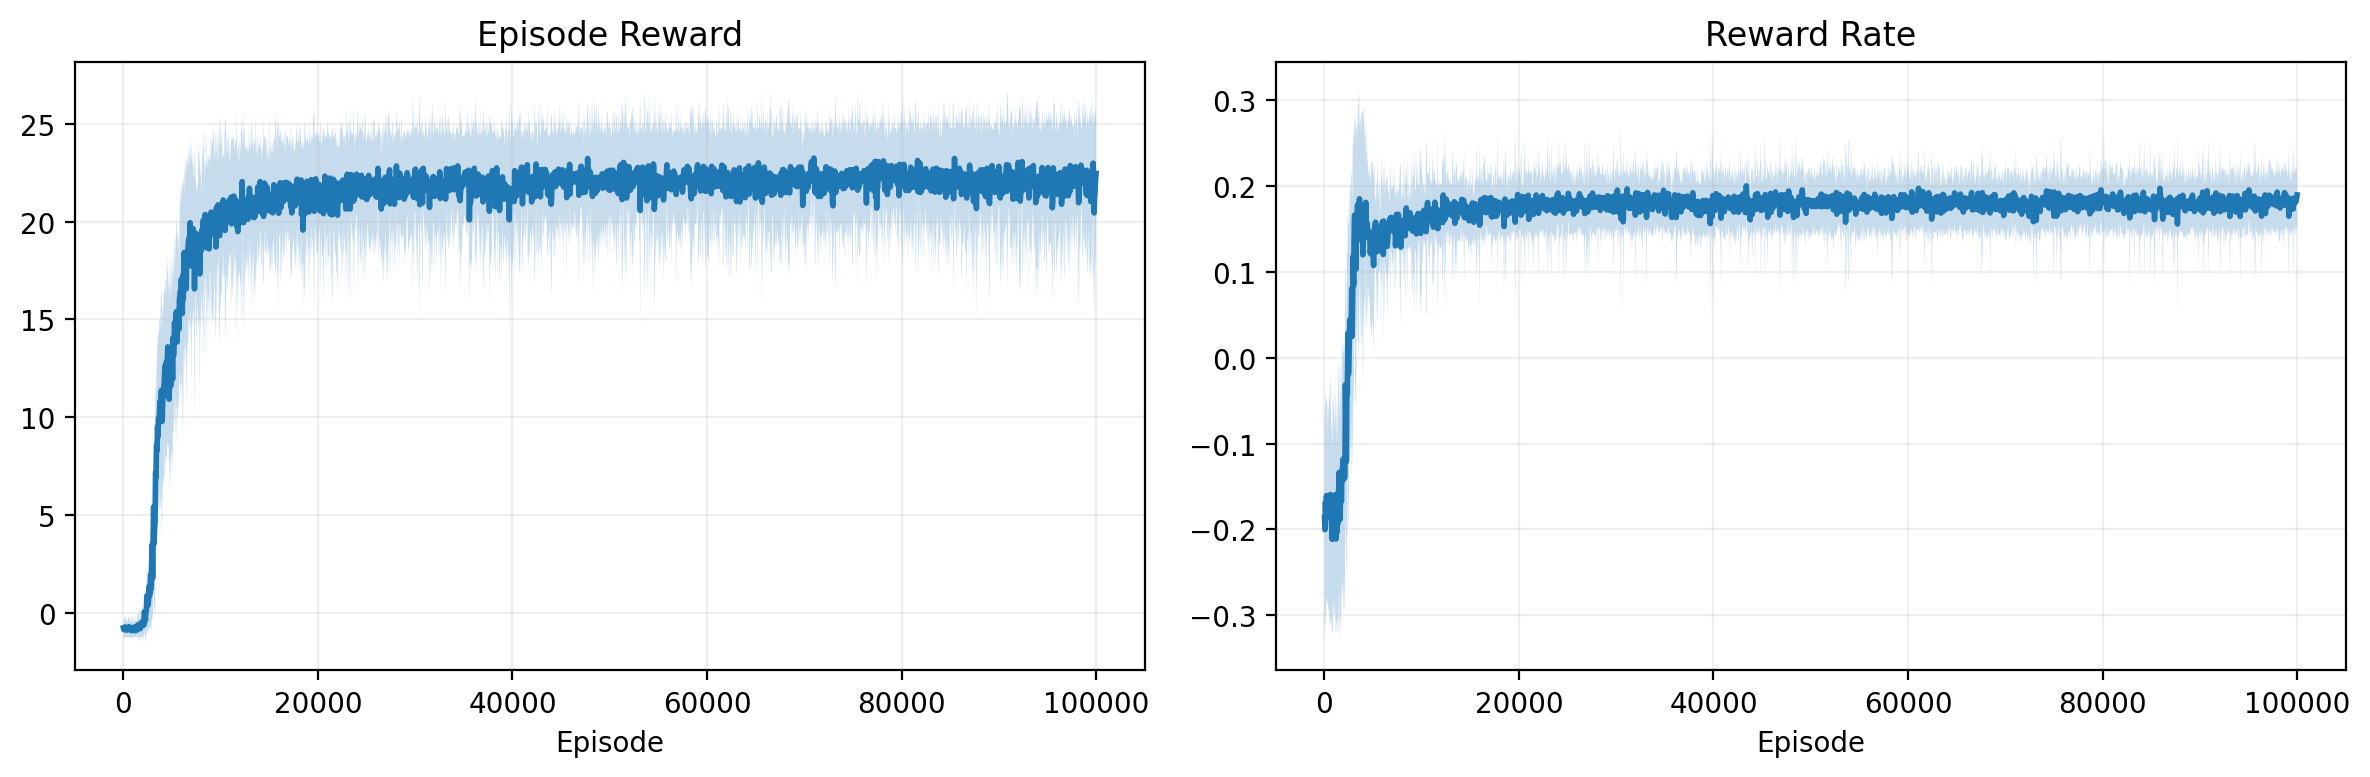
\includegraphics[width=0.92\linewidth]{images/EpisodicObjectivePPO.png}
    \caption[PPO with the episodic objective on Snake $5\times5$]{PPO trained
    on Snake $5\times5$ with the standard \emph{episodic} objective (the GAE
    done-mask left in place, so advantages do not cross episode boundaries).
    Left: total reward per episode; right: reward per step. Both curves are
    smoothed running averages over training ($100{,}000$ episodes), and the
    shaded band shows the spread of the raw per-episode values around the
    smoothed mean. Episode reward plateaus at roughly $22$ while the reward
    rate settles at $\approx 0.18$.}
    \label{fig:ppo-episodic}
\end{figure}

\begin{figure}[H]
    \centering
    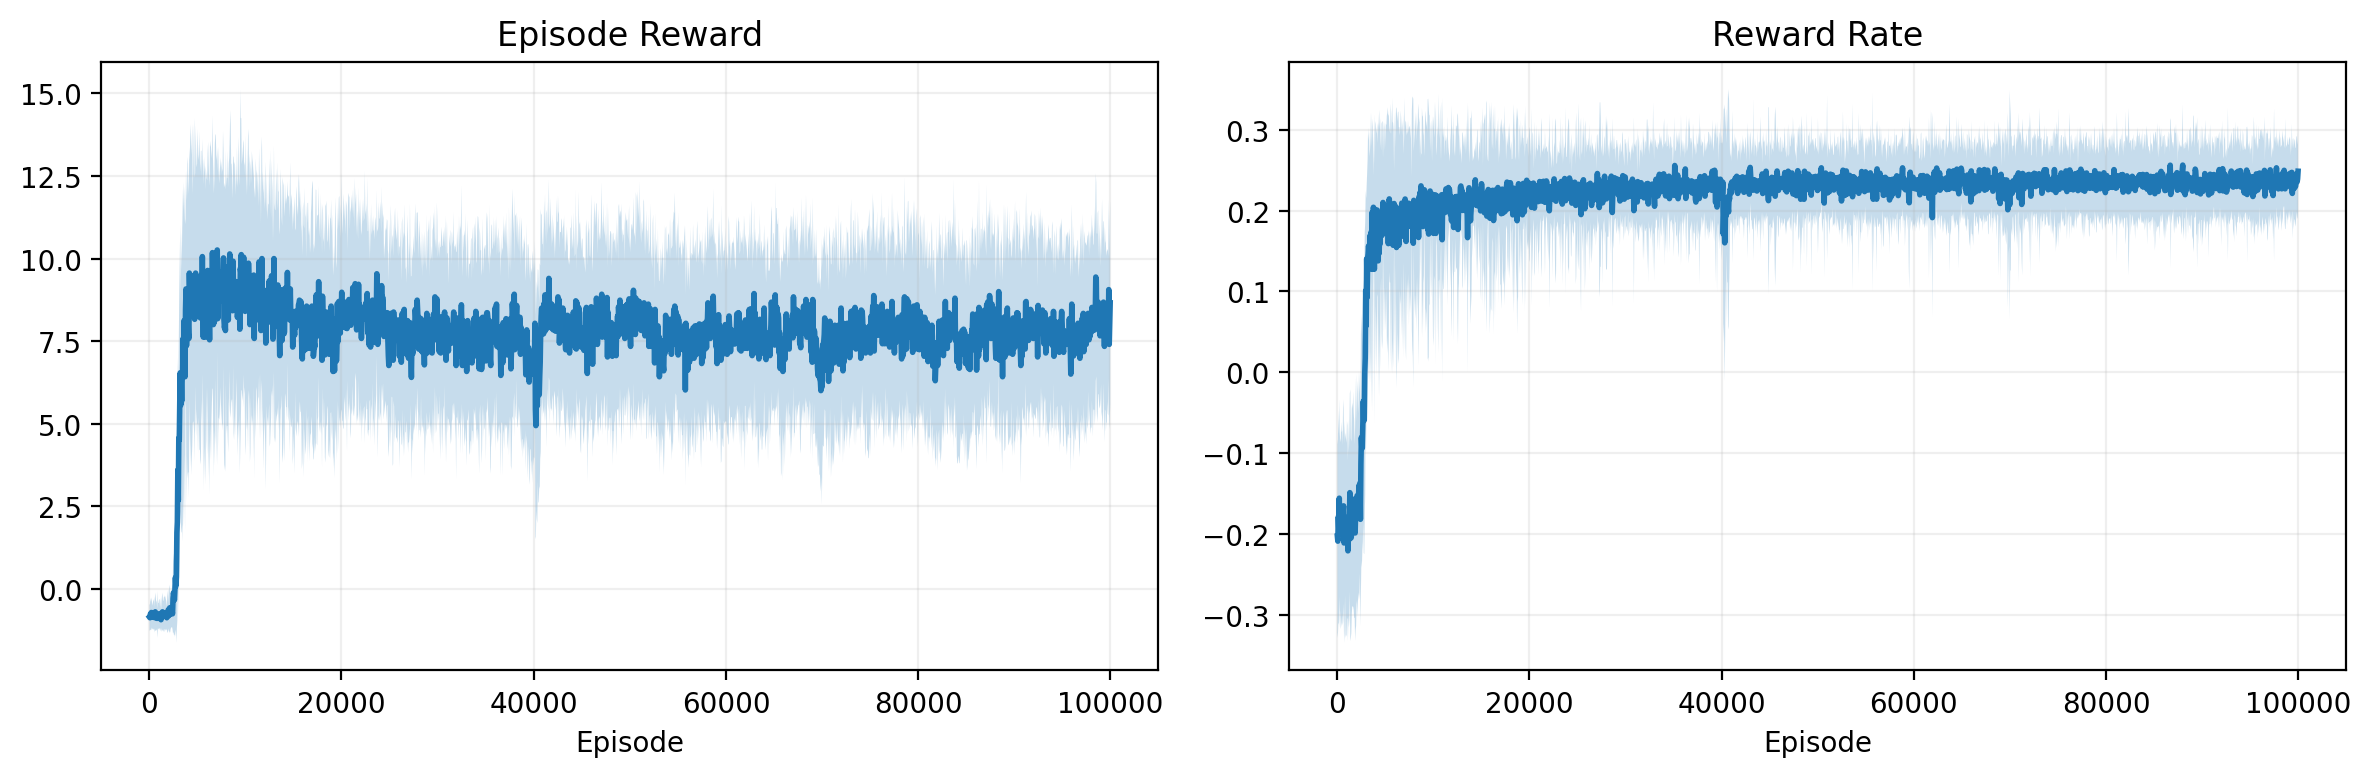
\includegraphics[width=0.92\linewidth]{images/ContinuousObjectivePPO.png}
    \caption[PPO with the continuing objective on Snake $5\times5$]{PPO
    trained on Snake $5\times5$ with the \emph{continuing} objective, no difference is made for terminal states, so the bootstrap and advantage
    recursion run through resets and the agent optimizes the uninterrupted
    reward stream, the same objective faced by the spiking agents. Axes and
    smoothing as in Figure~\ref{fig:ppo-episodic}. Relative to the episodic
    objective the picture inverts: episode reward plateaus far lower, at
    roughly $8$, while the reward rate rises to $\approx 0.24$, above the
    $\approx 0.18$ of the episodic agent. Each objective attains the higher
    value on the metric it actually optimizes.}
    \label{fig:ppo-continuous}
\end{figure}


The episodic and continuing objectives differ in exactly on the treatment of the
terminal transition in the advantage estimate, where the continuing variant lets the value
bootstrap across the episode boundary while the episodic variant masks it. Provided the critic
is reasonably accurate, how far this single difference propagates back into a trajectory is
largely governed by the value horizon $1/(1-\gamma)$. At $\gamma=0.99$ that horizon is roughly
$100$ steps, comparable to the length of a Snake episode, so the boundary treatment can reshape
the advantages of a large fraction of every trajectory. The two objectives then tend to pursue
different fixed points, one accumulating per-episode return and the other reward per step, and
the two performance metrics separate and can even move in opposite directions. At $\gamma=0.5$
the horizon shrinks to about $2$ steps, so the influence of the terminal transition decays
within a few steps and rarely reaches the body of an episode; masking it or not then makes
little practical difference, the episodic and continuing updates become nearly indistinguishable,
and the objectives, together with both metrics, largely converge. This reasoning does rest on the
value function being learned well enough for the bootstrap to behave as intended, an assumption we
expect to hold here because Snake $5\times5$ is predictable enough for the critic to be accurate;
in a task where the critic remained poor the picture could be less clean. Under that same
assumption the decoupled $\lambda=0.8$ would not, on its own, be expected to reopen the gap, as
discussed in Section~\ref{sec:practical-lambda}, it is primarily $\gamma$ that shapes \emph{what} is being optimized and hence
whether the episodic and continuing formulations differ appreciably. Were the critic largely
uninformative this separation would blur, and $\lambda$ could begin to influence the effective
objective; that this does not appear to happen here is itself consistent with the critic being
accurate on a task as predictable as Snake with the described rewards.

This also fixes the level at which the two curves meet. At $\gamma=0.5$ neither extreme strategy
is reachable, neither the long-survival behavior that maximizes per-episode return at
$\gamma=0.99$ (episode reward $\approx 22$) nor the most efficient reward-per-step policy
(reward rate $\approx 0.24$); a two-step horizon simply cannot represent either. Both objectives
instead settle on the same short-horizon compromise, an episode reward of about $13$ and a reward
rate of about $0.2$. Crucially, this is the \emph{same} $\gamma$ and $\lambda$ used by the
spiking rules, and the continuing PPO run lands essentially where symmetric e-prop does
(Section~\ref{sec:snake_lambda_comparison}). A strong gradient-based optimizer given the identical
short-horizon objective therefore reaches the same operating point as the local spiking rule,
which indicates that the spiking results are limited not by their credit-assignment machinery but
by the short objective horizon itself. This suggests that the headroom toward the higher reward rate seen at
$\gamma=0.99$ in this particular problem is recovered by lengthening the value horizon, that is by increasing $\gamma$.


\begin{figure}[H]
    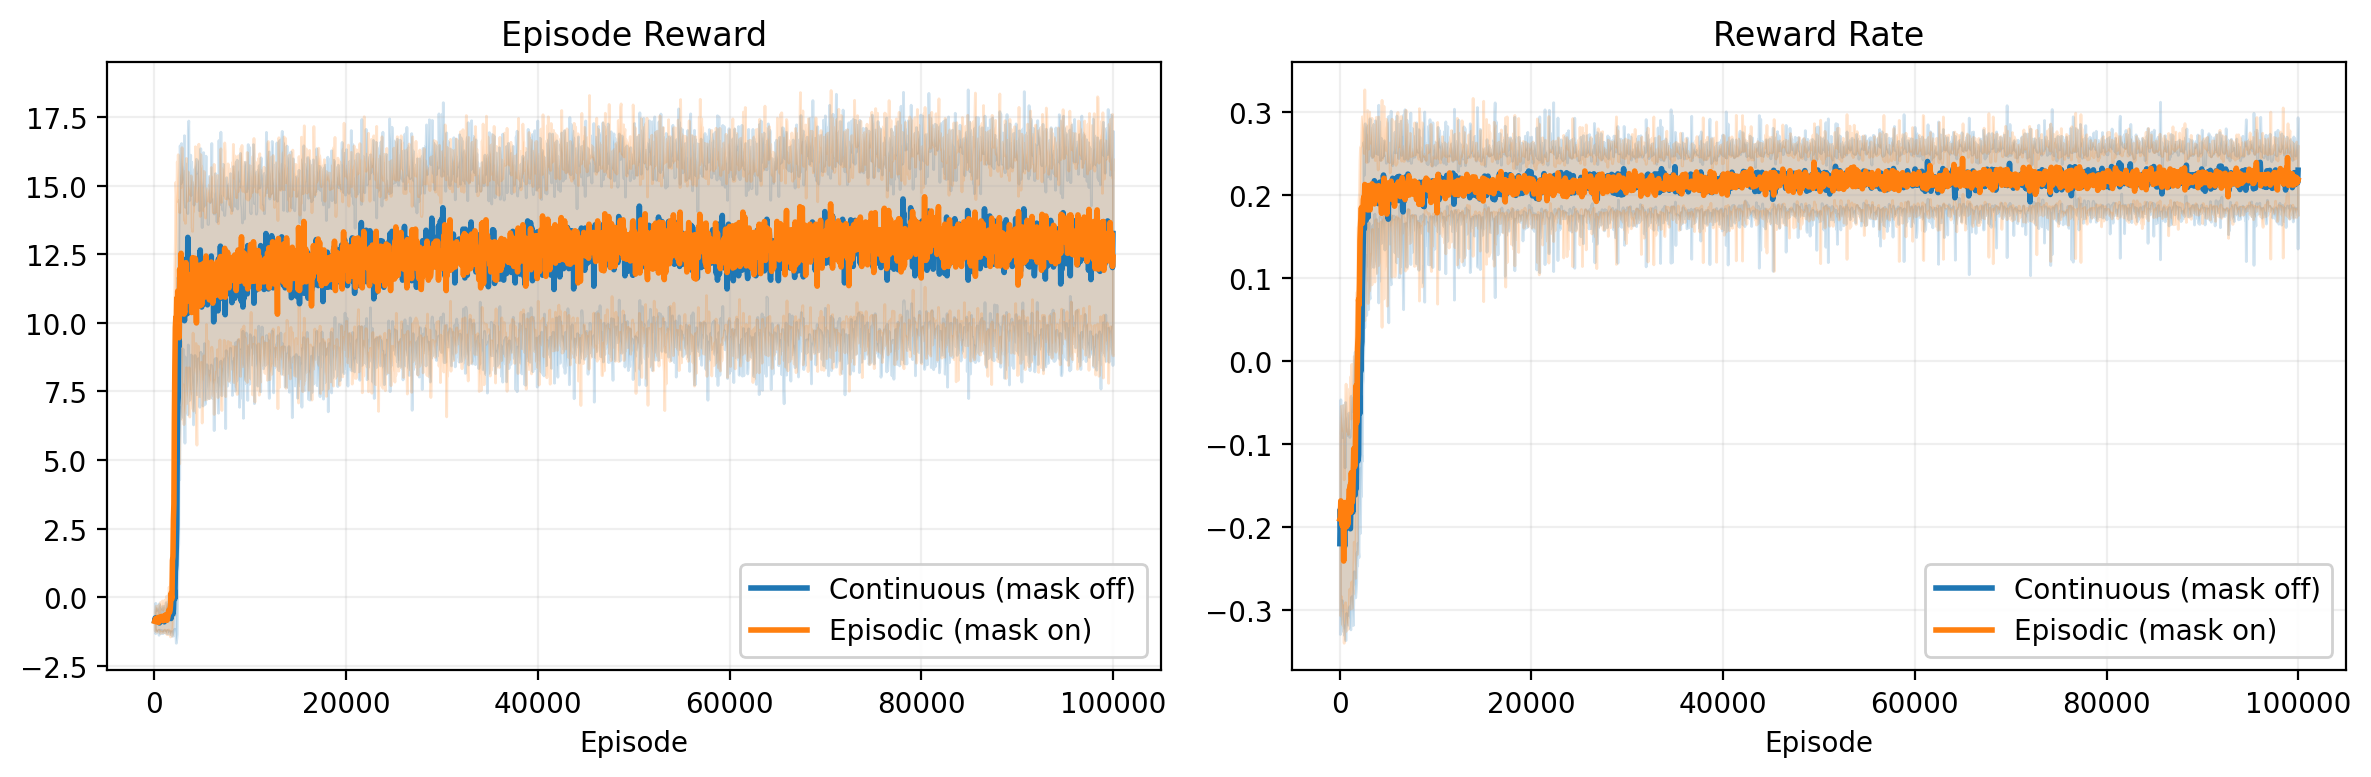
\includegraphics[width=\linewidth]{images/PPOComparison.png}
    \caption[Episodic vs.\ continuing PPO objective at $\gamma=0.5$, $\lambda=0.8$]{%
        PPO on Snake $5\times5$ under the episodic (terminal mask \emph{on}) and
        continuing (terminal mask \emph{off}) objectives, both with the decoupled
        setting $\gamma=0.5$, $\lambda=0.8$, overlaid on shared axes. \emph{Left:}
        episode reward. \emph{Right:} reward rate. Solid lines are the running mean
        and shaded bands the standard deviation across runs. In contrast to the
        $\gamma=0.99$ runs of Figures~\ref{fig:ppo-episodic} and~\ref{fig:ppo-continuous},
        the two objectives now nearly coincide on \emph{both} metrics.}
    \label{fig:ppo-episodic-vs-continuous}
\end{figure}

\section{Symmetric E-prop Dominance and Failure Case on Snake}
\label{sec:symmetric-failure}
\begin{figure}[H]
    \centering
    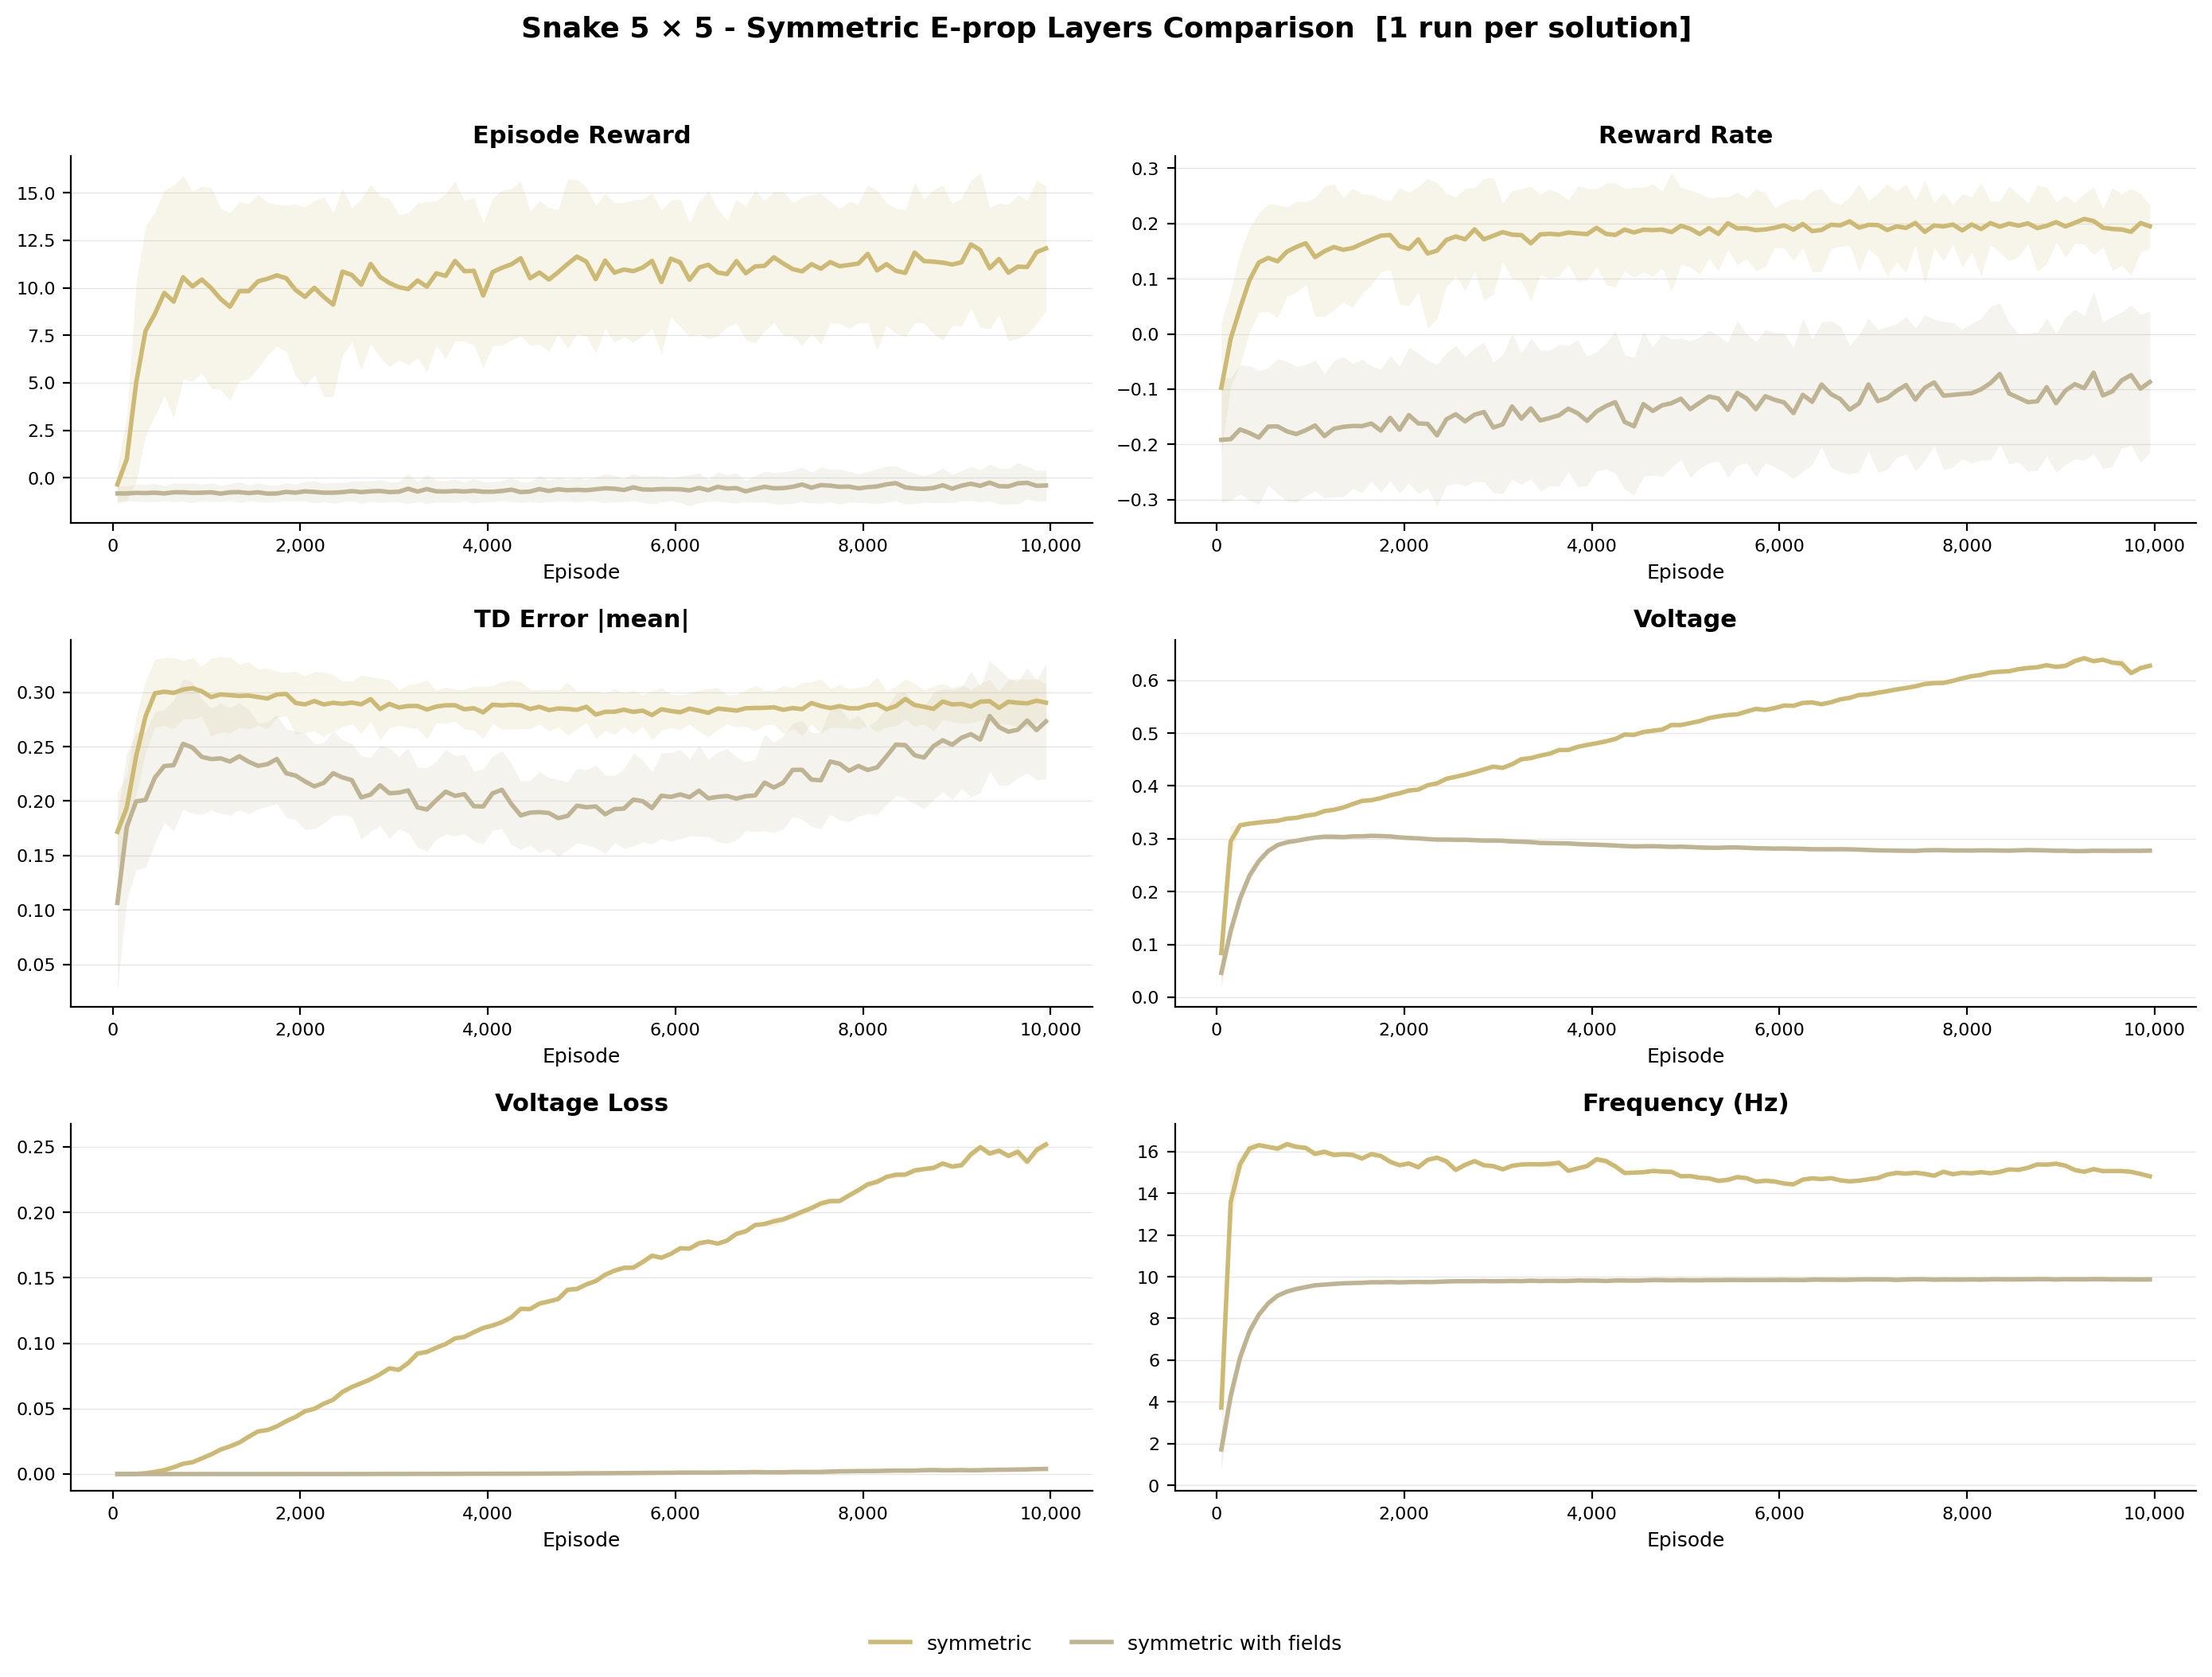
\includegraphics[width=1\linewidth]{images/SnakeSymmetric.png}
    \caption[Symmetric e-prop: with vs.\ without field layers]{Symmetric e-prop on Snake $5\times5$, with and without the per-head field layers
    (one run per configuration). Each panel tracks a quantity over $10{,}000$ episodes:
    episode reward, reward rate, mean absolute TD error, mean membrane voltage,
    voltage-regularization loss, and mean firing frequency (Hz). The plain symmetric variant
    attains the higher episode reward and reward rate together with the most favorable
    voltage and frequency statistics, whereas adding the value- and policy-field layers
    (\emph{symmetric with fields}) drives reward to near zero. The drop coincides with the
    longer causal path between input and output introduced by the field layers, which
    symmetric e-prop is unable to assign credit across reliably.}
    \label{fig:symmetric-layers}
\end{figure}
Of the configurations considered in this work, symmetric e-prop produces the strongest
overall behavior on Snake $5\times5$. As shown in Figure~\ref{fig:symmetric-layers}, it
converges to the highest episode reward and reward rate, and does so while maintaining the
most favorable voltage and frequency statistics, indicating a stable and well-regulated
spiking regime.

This advantage disappears as soon as the per-head field layers for the policy and value
outputs are introduced. The \emph{symmetric with fields} configuration suffers an absolute
drop in performance, with episode reward collapsing to near zero. The decisive factor is
the causal path length between input and output: the field layers lengthen this path, and
because the feedback weights of symmetric e-prop are tied to the forward output weights, the
credit assigned to non-connected neurons disappears. A
change that should be benign, namely adding expressive capacity to the read-out, instead breaks learning entirely.

The aggregate curves alone cannot tell us how the two configurations differ in behavior, only that they do. To understand what is actually lost when the field layers are introduced, Figures ~\ref{fig:qualitative_symmetric} and~\ref{fig:qualitative_symmetric_fields} examine a single representative episode from each configuration, revealing that the value function and policy both lose their structure entirely.

\begin{figure}[H]
    \centering
    \begin{subfigure}{0.538\linewidth}
        \centering
        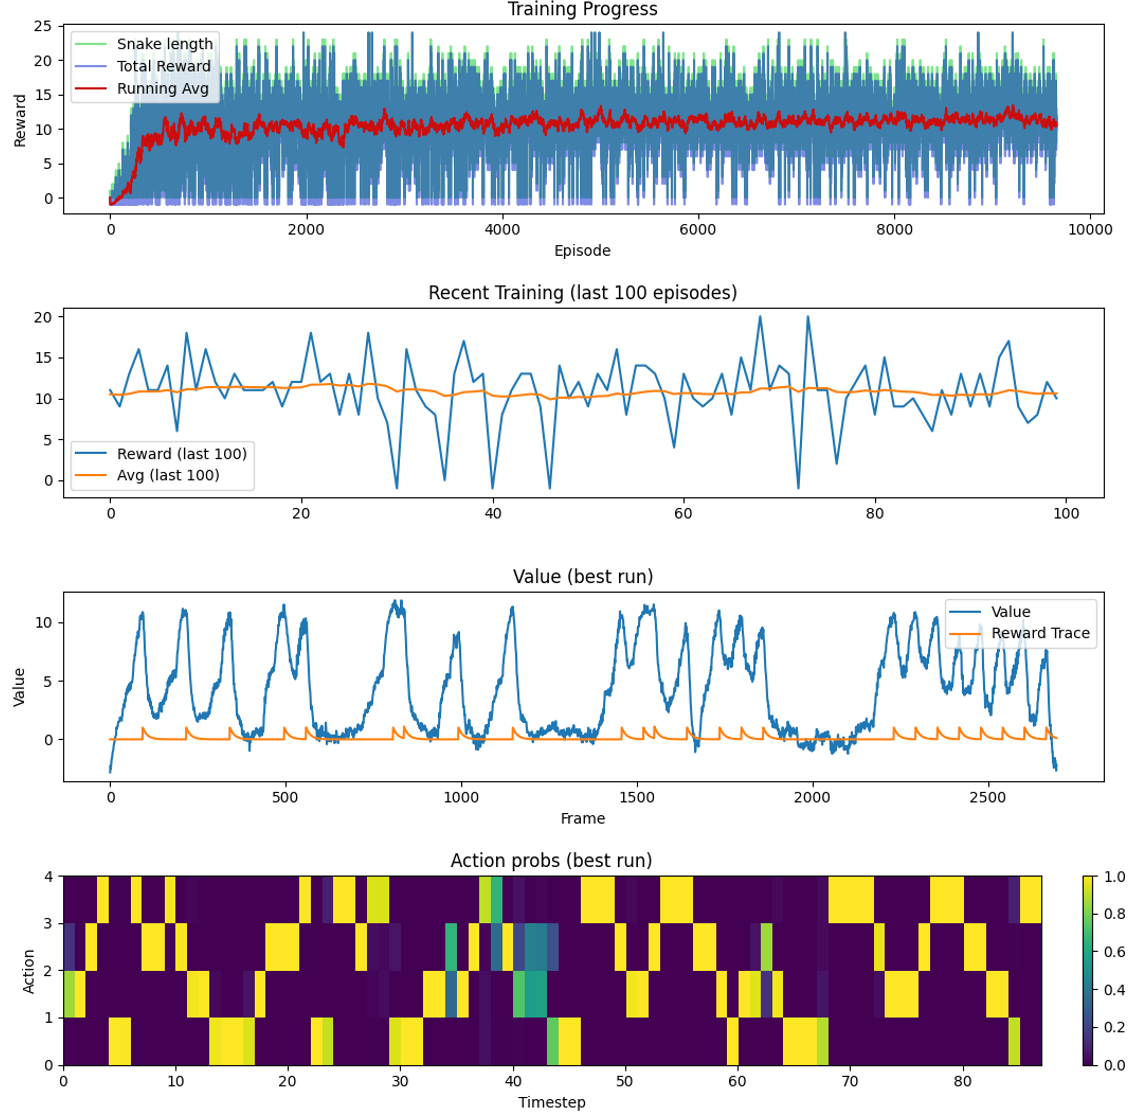
\includegraphics[width=\linewidth]{QualitativeSymmetric.png}
        \caption{Qualitative Symmetric}
        \label{fig:qualitative_symmetric}
    \end{subfigure}
    \hfill
    \begin{subfigure}{0.454\linewidth}
        \centering
        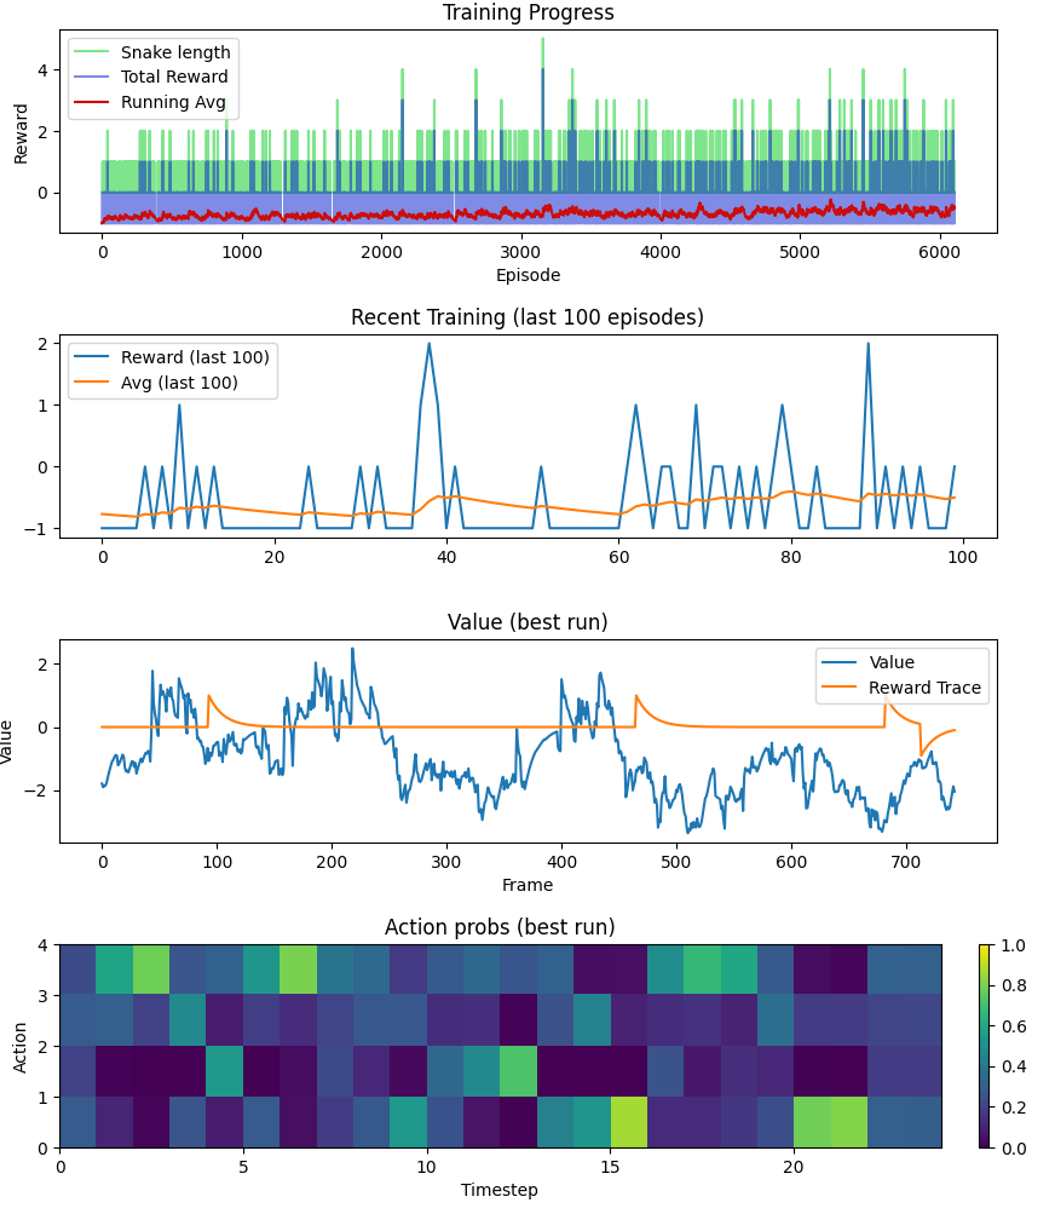
\includegraphics[width=\linewidth]{QualitativeSymmetricWithFields.png}
        \caption{Qualitative Symmetric With Fields}
        \label{fig:qualitative_symmetric_fields}
    \end{subfigure}
    
    \caption[Qualitative symmetric e-prop, field layers ablation]{Qualitative comparison of symmetric e-prop without (a) and with (b) the
    per-head field layers on Snake $5\times5$. From top to bottom each column shows: the
    training progress over all episodes (snake length, total reward, and running average);
    the reward over the most recent $100$ episodes against its running mean; the value
    estimate $V_t$ against the reward trace for the best run; and a heat map of the action
    probabilities through an episode. Without the field layers (a) the agent reaches
    greater snake lengths and rewards, its value trace is clearly structured, and its policy
    becomes close to deterministic (sharp light/dark bands); with the field layers (b)
    reward stays near zero, the value estimate is largely unstructured, and the policy
    remains diffuse.}
    \label{fig:qual-symmetric}
\end{figure}

Figure~\ref{fig:qual-symmetric} contrasts the two symmetric configurations on a single
representative run each. 
Without the field layers the agent produces long, reward-bearing episodes, a value
estimate with clear periodic structure, and an action distribution that sharpens into
near-deterministic choices. Once the field layers are introduced, the same diagnostics
degrade (reward collapses, the value trace loses its structure, and the policy stays
close to uniform), reinforcing the view that the longer credit path is responsible for the failure.

This failure is precisely what motivates the two alternative formulations studied in the
remainder of this chapter. The collapse is expected by the structure of symmetric e-prop, its feedback weights are
tied to the output weights, so if the majority of neurons do not have a connection to the output, then they do not receive any causal feedback information about the policy or value heads. This points to the property we
actually care about, namely a learning rule whose credit assignment scales gracefully with
causal path length. Two complementary ways of achieving it suggest themselves. The first is
to decouple the feedback pathway from the forward weights, as in random and adaptive e-prop,
where the learning signal is routed through fixed or independently learned feedback weights. 

The second, more radical option is to dispense with structured
feedback entirely, by treating each neuron as an independent stochastic actor
driven only by a global scalar signal and its own local action traces, changing the domain of the problem from a gradient routing problem to a noisy correlation problem.

\section{Distributed E-prop versus adaptive E-prop on Snake $5 \times 5$}
\label{sec:snake_comparison}

To assess how the different credit-assignment strategies behave on a fully observable
navigation task, we evaluate all variants on the Snake $5\times5$ problem over $10{,}000$
episodes, averaged over five independent runs. Figure~\ref{fig:snake_comparison} reports the
metrics introduced in Section~\ref{sec:reading-figures} for the configurations defined in
Table~\ref{tab:variant-naming}. In all cases the exploration variance $\sigma$ is held
fixed throughout training because the per-synapse variance
update of Section~\ref{subsec:exploration_variance} was not found to work reliably in practice and is
therefore excluded here. Shaded regions indicate the variability across runs.


\subsection{Comparison with $\lambda=0.8$}
\begin{figure}[h]
    \centering
    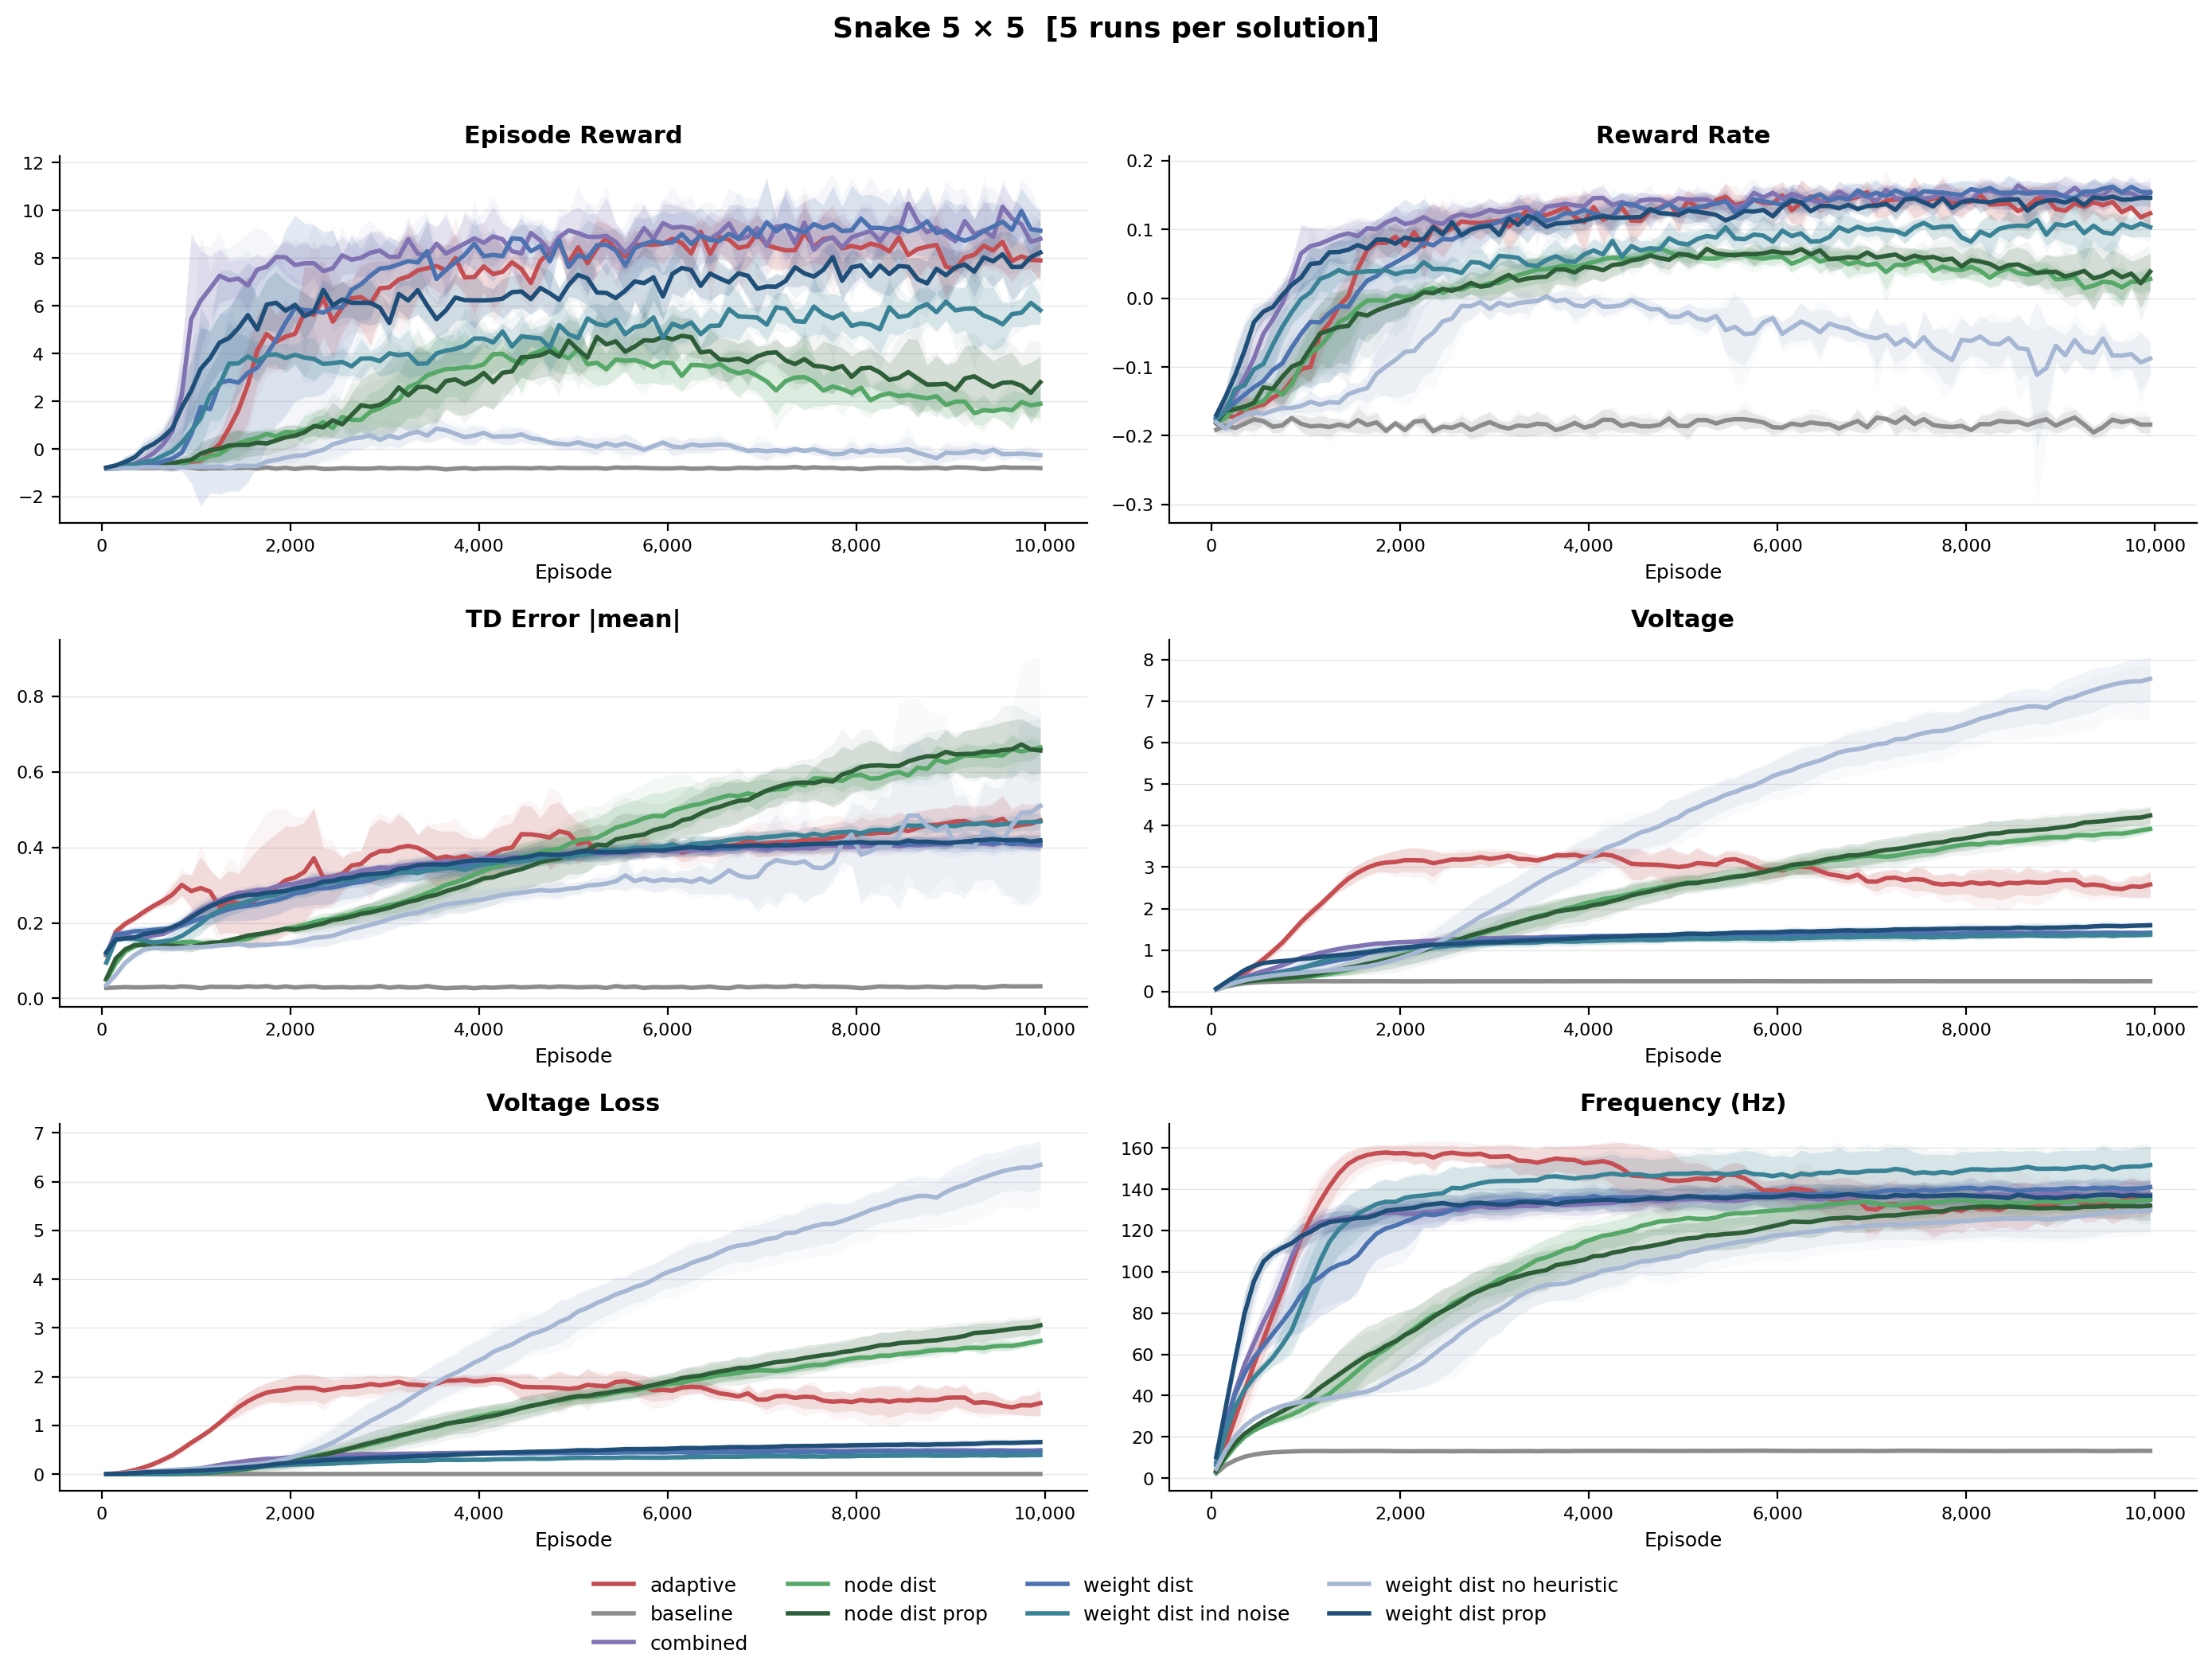
\includegraphics[width=\textwidth]{images/SnakeComparison.png}
    \caption[Credit-assignment variants on Snake $5\times5$]{Comparison of credit-assignment variants on the Snake $5\times5$ task over
    $10{,}000$ episodes. Each panel reports a different metric (episode reward, reward rate,
    mean absolute TD error, voltage, voltage loss, and frequency in Hz) for the configurations
    listed in the legend. Solid lines show the mean and shaded regions the variability across
    the five runs per configuration.}
    \label{fig:snake_comparison}
\end{figure}

\begin{figure}
    \centering
    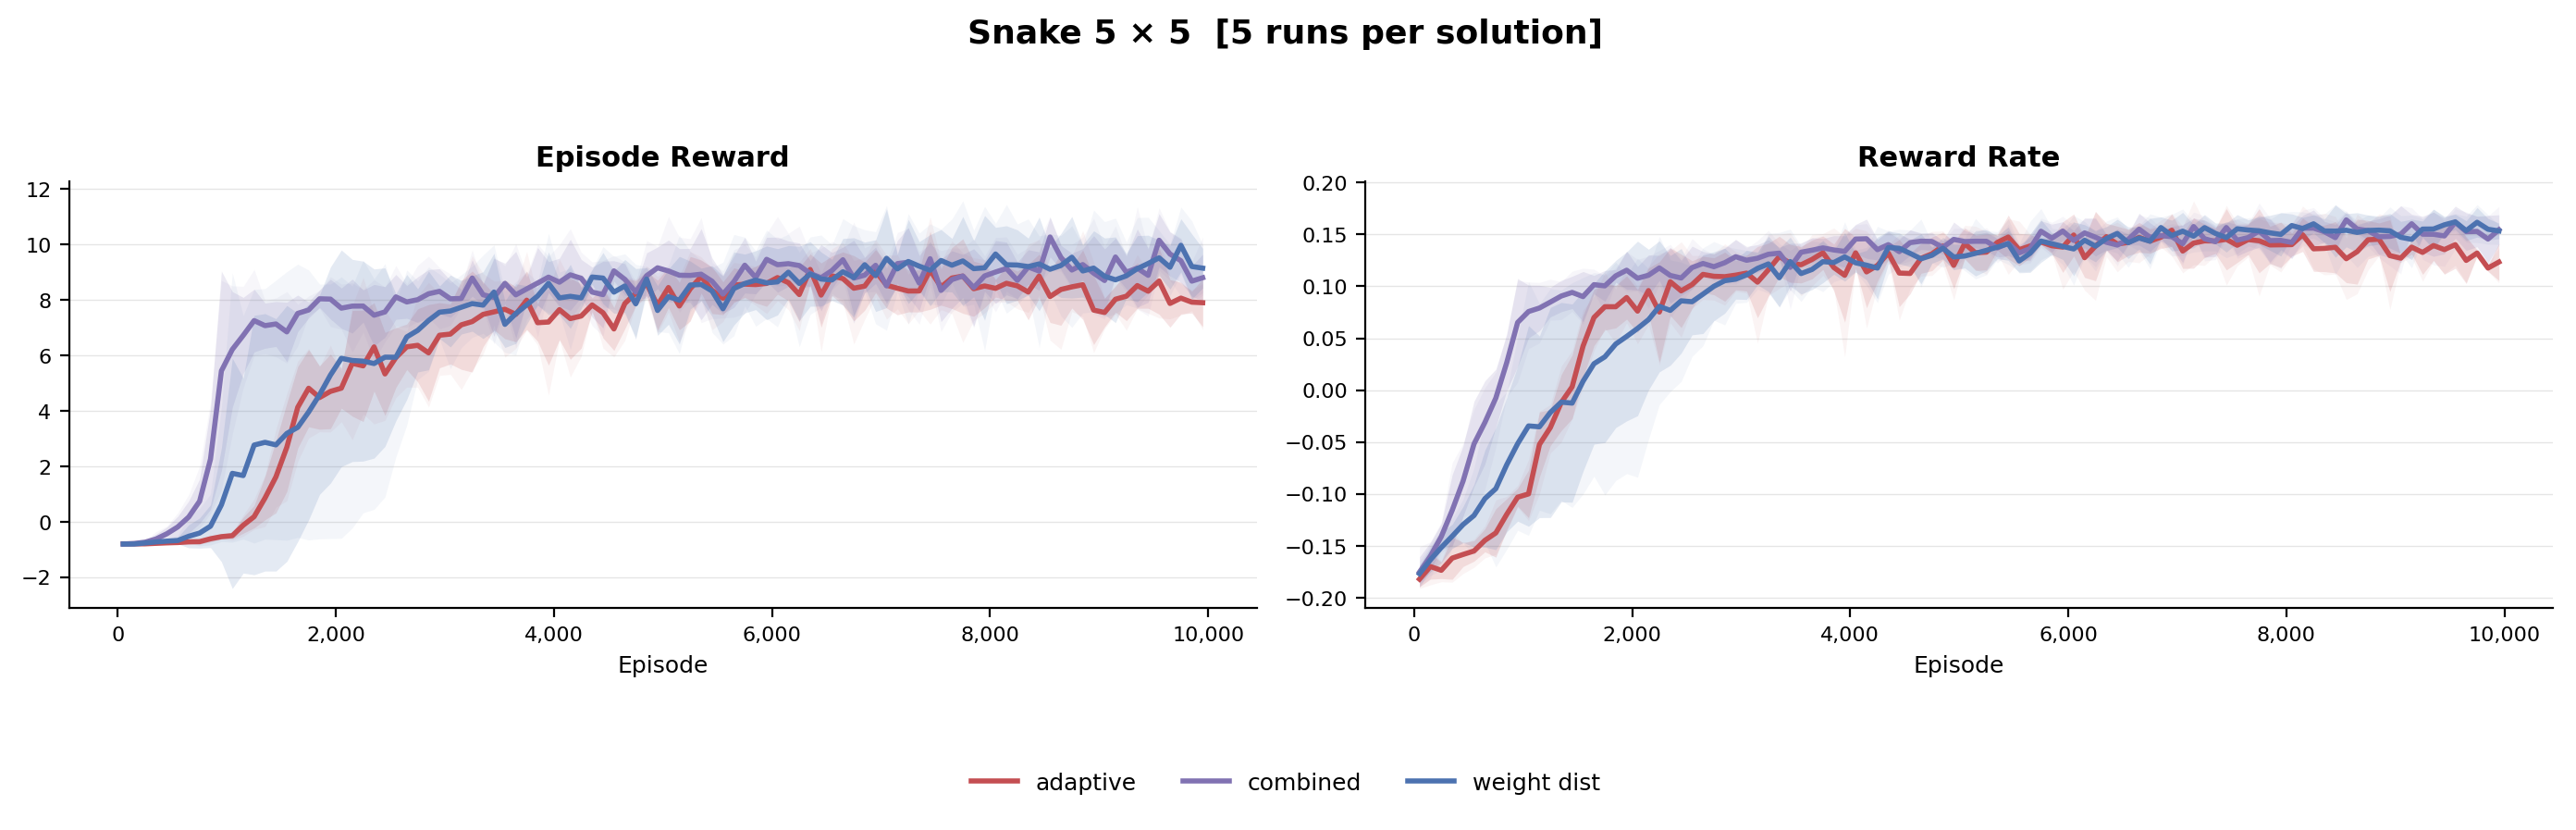
\includegraphics[width=1\linewidth]{SnakeTop3Comparison.png}
    \caption[Episode reward and reward rate, focused view (Snake, $5$ runs)]{%
    The two performance panels of Figure~\ref{fig:snake_comparison} (episode reward
    (left) and reward rate (right)) shown on their own for the three primary rules:
    adaptive (red), combined (purple) and weight dist (blue), on Snake $5\times5$
    with five independent runs each. Solid lines show the mean across runs and
    shaded bands the spread; the horizontal axis is the training episode. These
    panels are reproduced in isolation, away from the fuller diagnostic grid, so
    that the closely overlapping curves can be read more easily; the complete set of
    diagnostics and the accompanying discussion are given with
    Figure~\ref{fig:snake_comparison}.}
    \label{fig:placeholder}
\end{figure}


Before examining the individual metrics, it is worth stating the headline
result. Most variants learn the task successfully, converging to an episode
reward in the range of 8 to 10, but they differ substantially in how
quickly they do so, how stable their spiking dynamics are, and how well
their value functions track the actual return signal. The synaptic
perturbation variant \emph{weight dist} and the hybrid \emph{combined}
rule emerge as the strongest performers overall: \emph{combined} reaches
high reward faster than any other variant, while \emph{weight dist}
achieves the most stable final performance among the perturbation-based
rules, both maintaining low and well-regulated voltage throughout training.
Structured routing of the local policy signal has opposite effects depending
on the underlying estimator: it offers a modest improvement to the
neuron-perturbation variant \emph{node dist}, but disrupts the already
well-performing \emph{weight dist}, suggesting it is not universally
beneficial. The clearest failure case is \emph{weight dist no heuristic},
which demonstrates that the pseudo-derivative $\psi^t_j$ is not an optional
refinement but an essential component of the learning rule. The
\emph{adaptive} variant learns more slowly and shows signs of early
instability, but eventually reaches comparable performance. The following
analysis unpacks the mechanisms behind these differences metric by metric.

\paragraph{Episode Reward and Reward Rate.}

As a reference point, the \emph{baseline} configuration, in which only the output weights
are trained and the recurrent dynamics are left fixed, makes essentially no progress: its
episode reward stays close to zero throughout training and shows no discernible trend in
either direction. This confirms that solving the task requires shaping the recurrent dynamics
themselves, and that a trainable read-out on top of fixed recurrent activity carries
negligible learning capacity in this setting. It also provides a floor against which the
remaining variants can be read: any configuration that departs clearly from this flat
trajectory is, at minimum, propagating a usable learning signal into the recurrent weights.

Most variants learn the task successfully, converging to an episode reward in the range of
$8$ to $10$. The variant \emph{combined} stands out for its fast early improvement, reaching a
high reward well before the others, while \emph{weight dist} achieves the strongest
and most stable final performance among the perturbation-based variants. The \emph{adaptive} variant learns more slowly at first but eventually catches up to a comparable reward.

Two results within this comparison are particularly worth noting. First, \emph{weight dist} substantially outperforms \emph{node dist} despite the two using the same
number of independent stochastic perturbation sources, namely one Gaussian sample per
postsynaptic neuron in both cases (see Section~\ref{subsec:synaptic_perturbation}). The gap
between them is therefore not attributable to a variance difference, since variance is
approximately matched, and must instead stem from the bias introduced by the neuron-level
variant's shared credit: every synapse onto a given neuron receives an identical
perturbation trace regardless of whether that synapse's presynaptic neuron was actually
active, whereas the synaptic variant's effective perturbation $\varepsilon^t_{ji}z^t_i$ is
gated by presynaptic firing and therefore only contributes to a synapse's credit trace when
that synapse's presynaptic neuron actually fired. One plausible explanation for the size of
this gap, which we have not verified further and present here only as a working hypothesis,
is that this gating makes the synaptic perturbation trace inherently more reflective of the
network's actual causal activity pattern: a synapse is only perturbed, and therefore only
credited or discredited, at moments when it could plausibly have contributed to the
postsynaptic neuron's behavior, whereas the neuron-level trace accumulates noise
irrespective of which specific synapses were in a position to act. This remains a hypothesis, and a more direct test would be needed to confirm it.

Second, structured routing of the local policy signal has \emph{opposite} effects on the two
perturbation types. For the neuron-level estimator, \emph{node dist prop} performs
slightly better, on average over the five runs, than its unrouted counterpart \emph{node
dist}, suggesting that the additional structured information helps compensate, at least
partially, for the coarseness of the underlying credit signal. For the synaptic estimator,
however, structured routing is clearly detrimental: \emph{weight dist prop} learns quickly
at first, even appearing briefly competitive with \emph{weight dist}, but then stalls
for an extended period, and although it shows some recovery later in training it ends clearly
below the unrouted \emph{weight dist}. This asymmetry suggests that structured routing
is not uniformly beneficial, but instead interacts differently depending on how reliable the
underlying local estimator already is: it appears to help an estimator that is already biased
and has comparatively little to lose, while it appears to disrupt an estimator that was
already performing well, plausibly by introducing an additional, only partially aligned source
of signal that the optimization must reconcile with the existing perturbation-based update.

A further ablation isolates the role of the pseudo-derivative $\psi^t_j$ in the eligibility
trace. The \emph{weight dist no heuristic} configuration is identical to \emph{weight dist} except that it removes the surrogate-derivative factor $\psi^t_j$, retaining only the
filtered presynaptic spike train $\bar{z}^t_i$, with no postsynaptic
gating. Among the configurations that train the recurrent and input weights, it is the worst
performer by a wide margin, attaining the lowest episode reward and reward rate and falling
well short of every other recurrent learning variant. This suggests that the pseudo-derivative is not an
optional refinement but an essential component of the learning rule: by restricting credit to
moments when the postsynaptic neuron is close to its firing threshold, $\psi^t_j$ keeps the
perturbation-based update aligned with the network's causal activity, and without it the credit
signals degrade to the point where they are unable to train the network.

\paragraph{TD Error.}
Before discussing the curves themselves, it is worth being explicit about how much weight
this metric can bear. A value function that has learned a genuinely useful predictive representation need not produce
a smaller TD error than a flatter, less informative one: the magnitude of $\delta_t$ reflects
the moment-to-moment mismatch between the value estimate and a bootstrapped, trace-based
target, not the long-run accuracy of the prediction, and a critic that barely moves from a
constant baseline can trivially produce small errors against a slowly varying trace without
having learned anything useful. We therefore do not treat the TD error as a direct proxy for
critic quality in what follows. The one use we consider defensible, with some caution, is as a
coarse indicator of \emph{instability}: a TD error that grows steadily or fluctuates with
increasing magnitude over training is at least consistent with a critic whose internal
dynamics are drifting, even though a low or flat TD error cannot, by the
same logic, be read as positive evidence of a good critic. Even this weaker reading should be
treated with caution, which is precisely why we
complement this quantitative metric with the qualitative value-trace inspection introduced in Section~\ref{sec:value-traces}.

With that caveat in mind, we limit ourselves to comparative observations. The adaptive
variant shows signs of instability in its TD error early in training, with an initial rise
and noticeable fluctuation before it settles onto a plateau. This aligns with the qualitative
value traces we will see in \ref{fig:value-trace-progression-snake}, where adaptive e-prop appears to struggle more
than the perturbation variants with learning the value function. The perturbation-based variants
follow a visibly different profile, with a TD error that grows more gradually over the course
of training, though we do not read anything further into this beyond the difference in shape.
The synaptic variants \emph{weight dist} and \emph{combined} keep their TD error
comparatively low and stable throughout. Across all configurations we do not observe a runaway
explosion in the TD error, which is consistent with the caveat above: this metric is better
suited to flagging instability than to certifying the quality of a learned value function.

\paragraph{Voltage and Voltage Loss.}
The spiking dynamics again split along the same lines as the reward results, with the
node-perturbation and synaptic families behaving very differently. The two node-perturbation
variants, \emph{node dist} and \emph{node dist prop}, both show a continuously increasing
membrane voltage and voltage loss throughout training, drifting to the highest values among
the variants that learn the task. Structured routing makes little difference here: the routed
and unrouted versions track one another closely, so the prop variants are only marginally
increased relative to their base counterparts. The adaptive variant displays a characteristic
early surge in voltage that subsequently relaxes, settling back towards a moderate level. By
contrast, the synaptic variants \emph{weight dist} and \emph{weight dist prop}, together
with \emph{combined}, hold low and stable voltage and voltage loss across the entire run,
reflecting tightly controlled spiking activity. The clearest outlier is \emph{weight dist no
heuristic}: with the pseudo-derivative removed, its membrane voltage diverges, growing without
settling for the entire run and reaching values well beyond every other configuration.

\paragraph{Frequency.}
The firing frequency of all variants increases during training and converges to a broadly
similar band of roughly $130$ to $150$ Hz, which is very high, regardless of which credit-assignment strategy is
used. The \emph{adaptive} variant again
rises fastest and overshoots the eventual range early before settling, mirroring its early
voltage surge, whereas the node-perturbation variants approach the common range more gradually. The variant \emph{weight dist no heuristic} is no exception here, converging to the same high band as the
others, so frequency does little to distinguish it despite its poor reward and diverging voltage.


\begin{figure}[H]
    \centering
    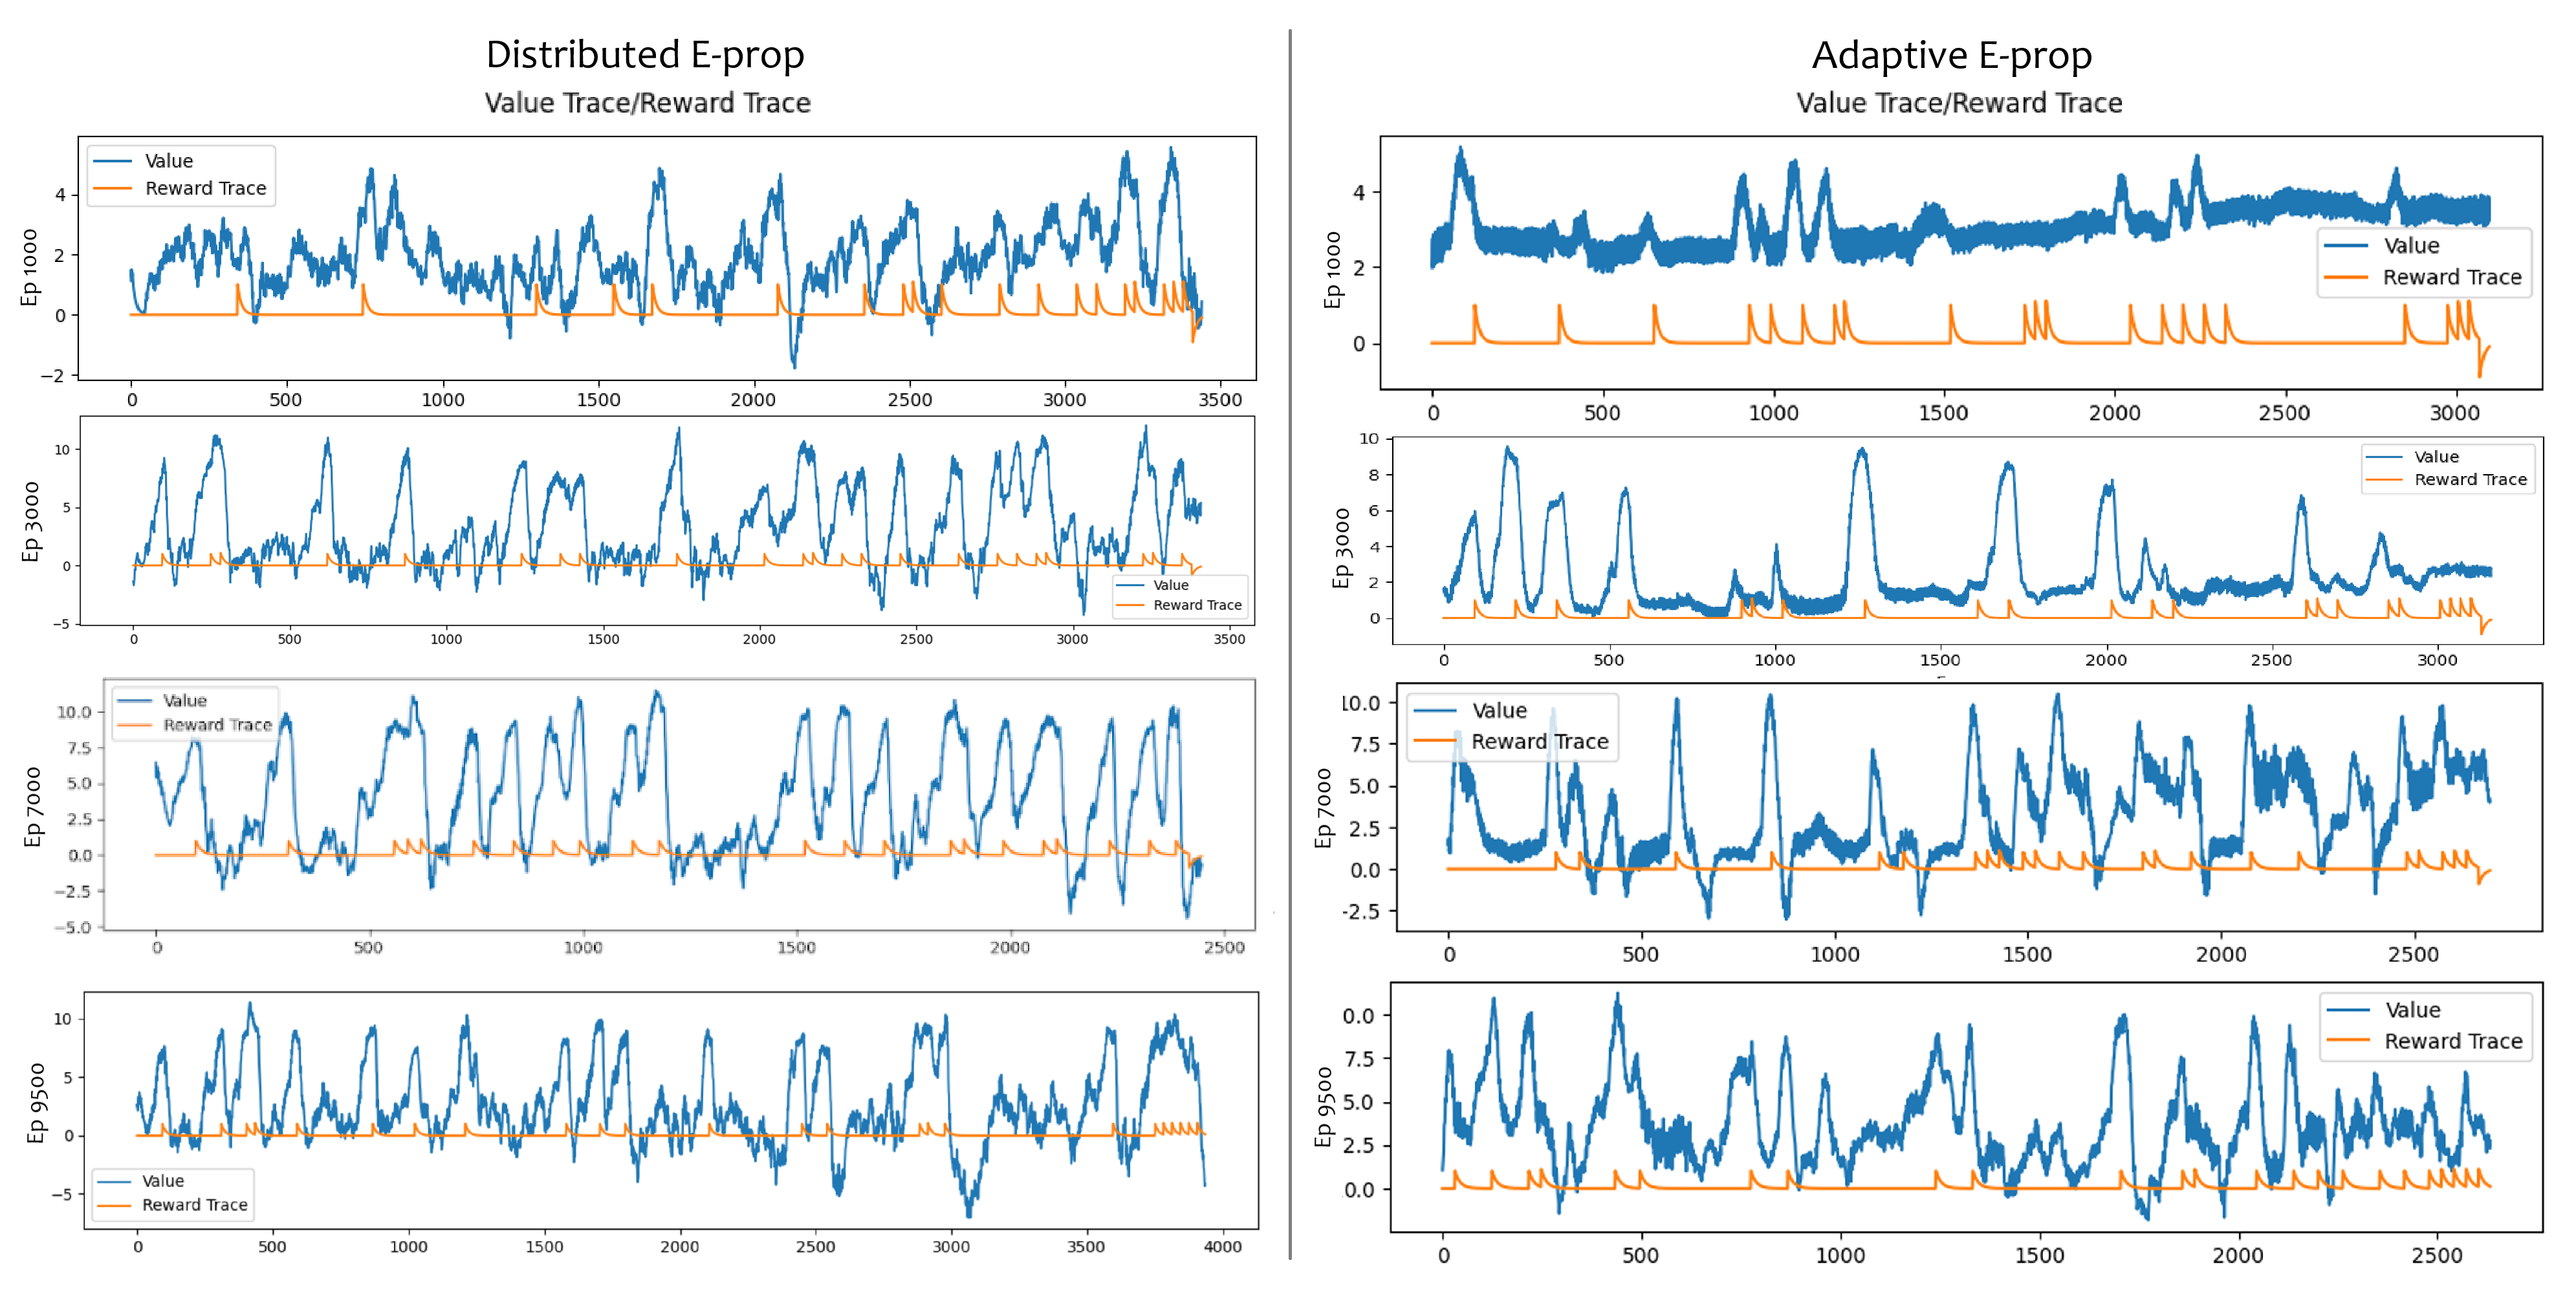
\includegraphics[width=1\linewidth]{images/SnakeValueTraceComparison.png}
    \caption[Value and reward traces on Snake]{%
    Value and reward traces for distributed e-prop (left) and adaptive e-prop
    (right) on Snake. The figure combines two distinct notions of time, which
    the axes deliberately keep separate. Reading down a column, each row is a
    snapshot taken at a different point in training (episodes $1000$, $3000$,
    $7000$ and $9500$ of the same run) so successive rows show how the value
    function develops as learning progresses; a column is not a single
    continuous trace. Reading across a panel, the horizontal axis is the
    frame number within a single game played at that checkpoint, and it necessarily
    restarts from zero in every panel; because games last for different numbers of
    frames, the panels span different frame counts and so differ in width. In every
    panel the blue curve is the critic's value estimate and the orange curve is the
    reward trace, whose spikes mark the frames at which reward is received. The
    vertical scales are independent from panel to panel, the magnitude of the
    learned value grows over training, and each panel is scaled to its own range so
    that the within-game structure remains visible.
    }
    \label{fig:value-trace-progression-snake}
\end{figure}

Read from top to bottom, Figure~\ref{fig:value-trace-progression-snake} shows how the relationship between the
value trace and the reward signal is expected to evolve as learning proceeds, following the
qualitative signature introduced in Section~\ref{sec:reading-figures}: an early value estimate
that tracks reward only loosely and without anticipation, gradually giving way to sharper,
structured excursions that lead reward events instead of trailing them, rising ahead of an
apple being collected and falling ahead of a collision. We use this progression throughout the
chapter to argue that a variant has learned a genuinely predictive value function.

A closer comparison between the two variants in Figure~\ref{fig:value-trace-progression-snake} reveals a
qualitative difference beyond this general progression. Although it is read from a single run
per variant, and is therefore illustrative, it is consistent across
the episodes shown. The value trace learned by distributed e-prop settles into a clean and
highly predictable shape, we can see how the estimate rises gradually, reaches a peak shortly before a reward
event, and then descends precisely at the moment the reward is received, closely tracking the
true timing of the underlying event. Adaptive e-prop takes considerably longer to adjust during
training, and even after extended learning it never develops this same predictive shape. Its
value trace remains comparatively noisier and less consistently timed, lacking the smooth
rise-and-fall structure that distributed e-prop shows in relation to reward delivery. This
contrast suggests that distributed e-prop arrives at a sharper and more temporally precise value
representation, while adaptive e-prop's critic remains comparatively underdeveloped within the
same training budget, consistent with the early instability seen in its TD error in Figure~\ref{fig:snake_comparison}.

\subsection{Lambda Comparison}
\label{sec:snake_lambda_comparison}

The experiments presented so far in this chapter have used a single fixed
value of the decay factor $\lambda$ from the TD($\lambda$) algorithm
throughout training. We now turn to the sensitivity of each learning rule
to this choice. As discussed in Section~\ref{sec:practical-lambda},
$\lambda$ sets the effective horizon, of order $1/(1-\lambda)$ steps, over
which a temporal-difference error is distributed back onto past
contributions, so small $\lambda$ concentrates credit near the present
action, while $\lambda$ close to 1 holds much earlier actions accountable,
at the cost of a higher-variance credit trace. This tradeoff is a property
of TD($\lambda$) in general, but how severely a given learning rule is
affected by it, and over what range of $\lambda$ it remains usable at all,
is an empirical question specific to how that rule constructs its update
from the credit trace. We examine this here on the Snake $5\times5$ task,
and return to it on the Pac-Man randomized layouts problem in
Section~\ref{sec:lambda_comparison}, since comparing the two will turn out
to be informative precisely because the two tasks produce different
answers.

\begin{figure}[htbp]
    \centering
    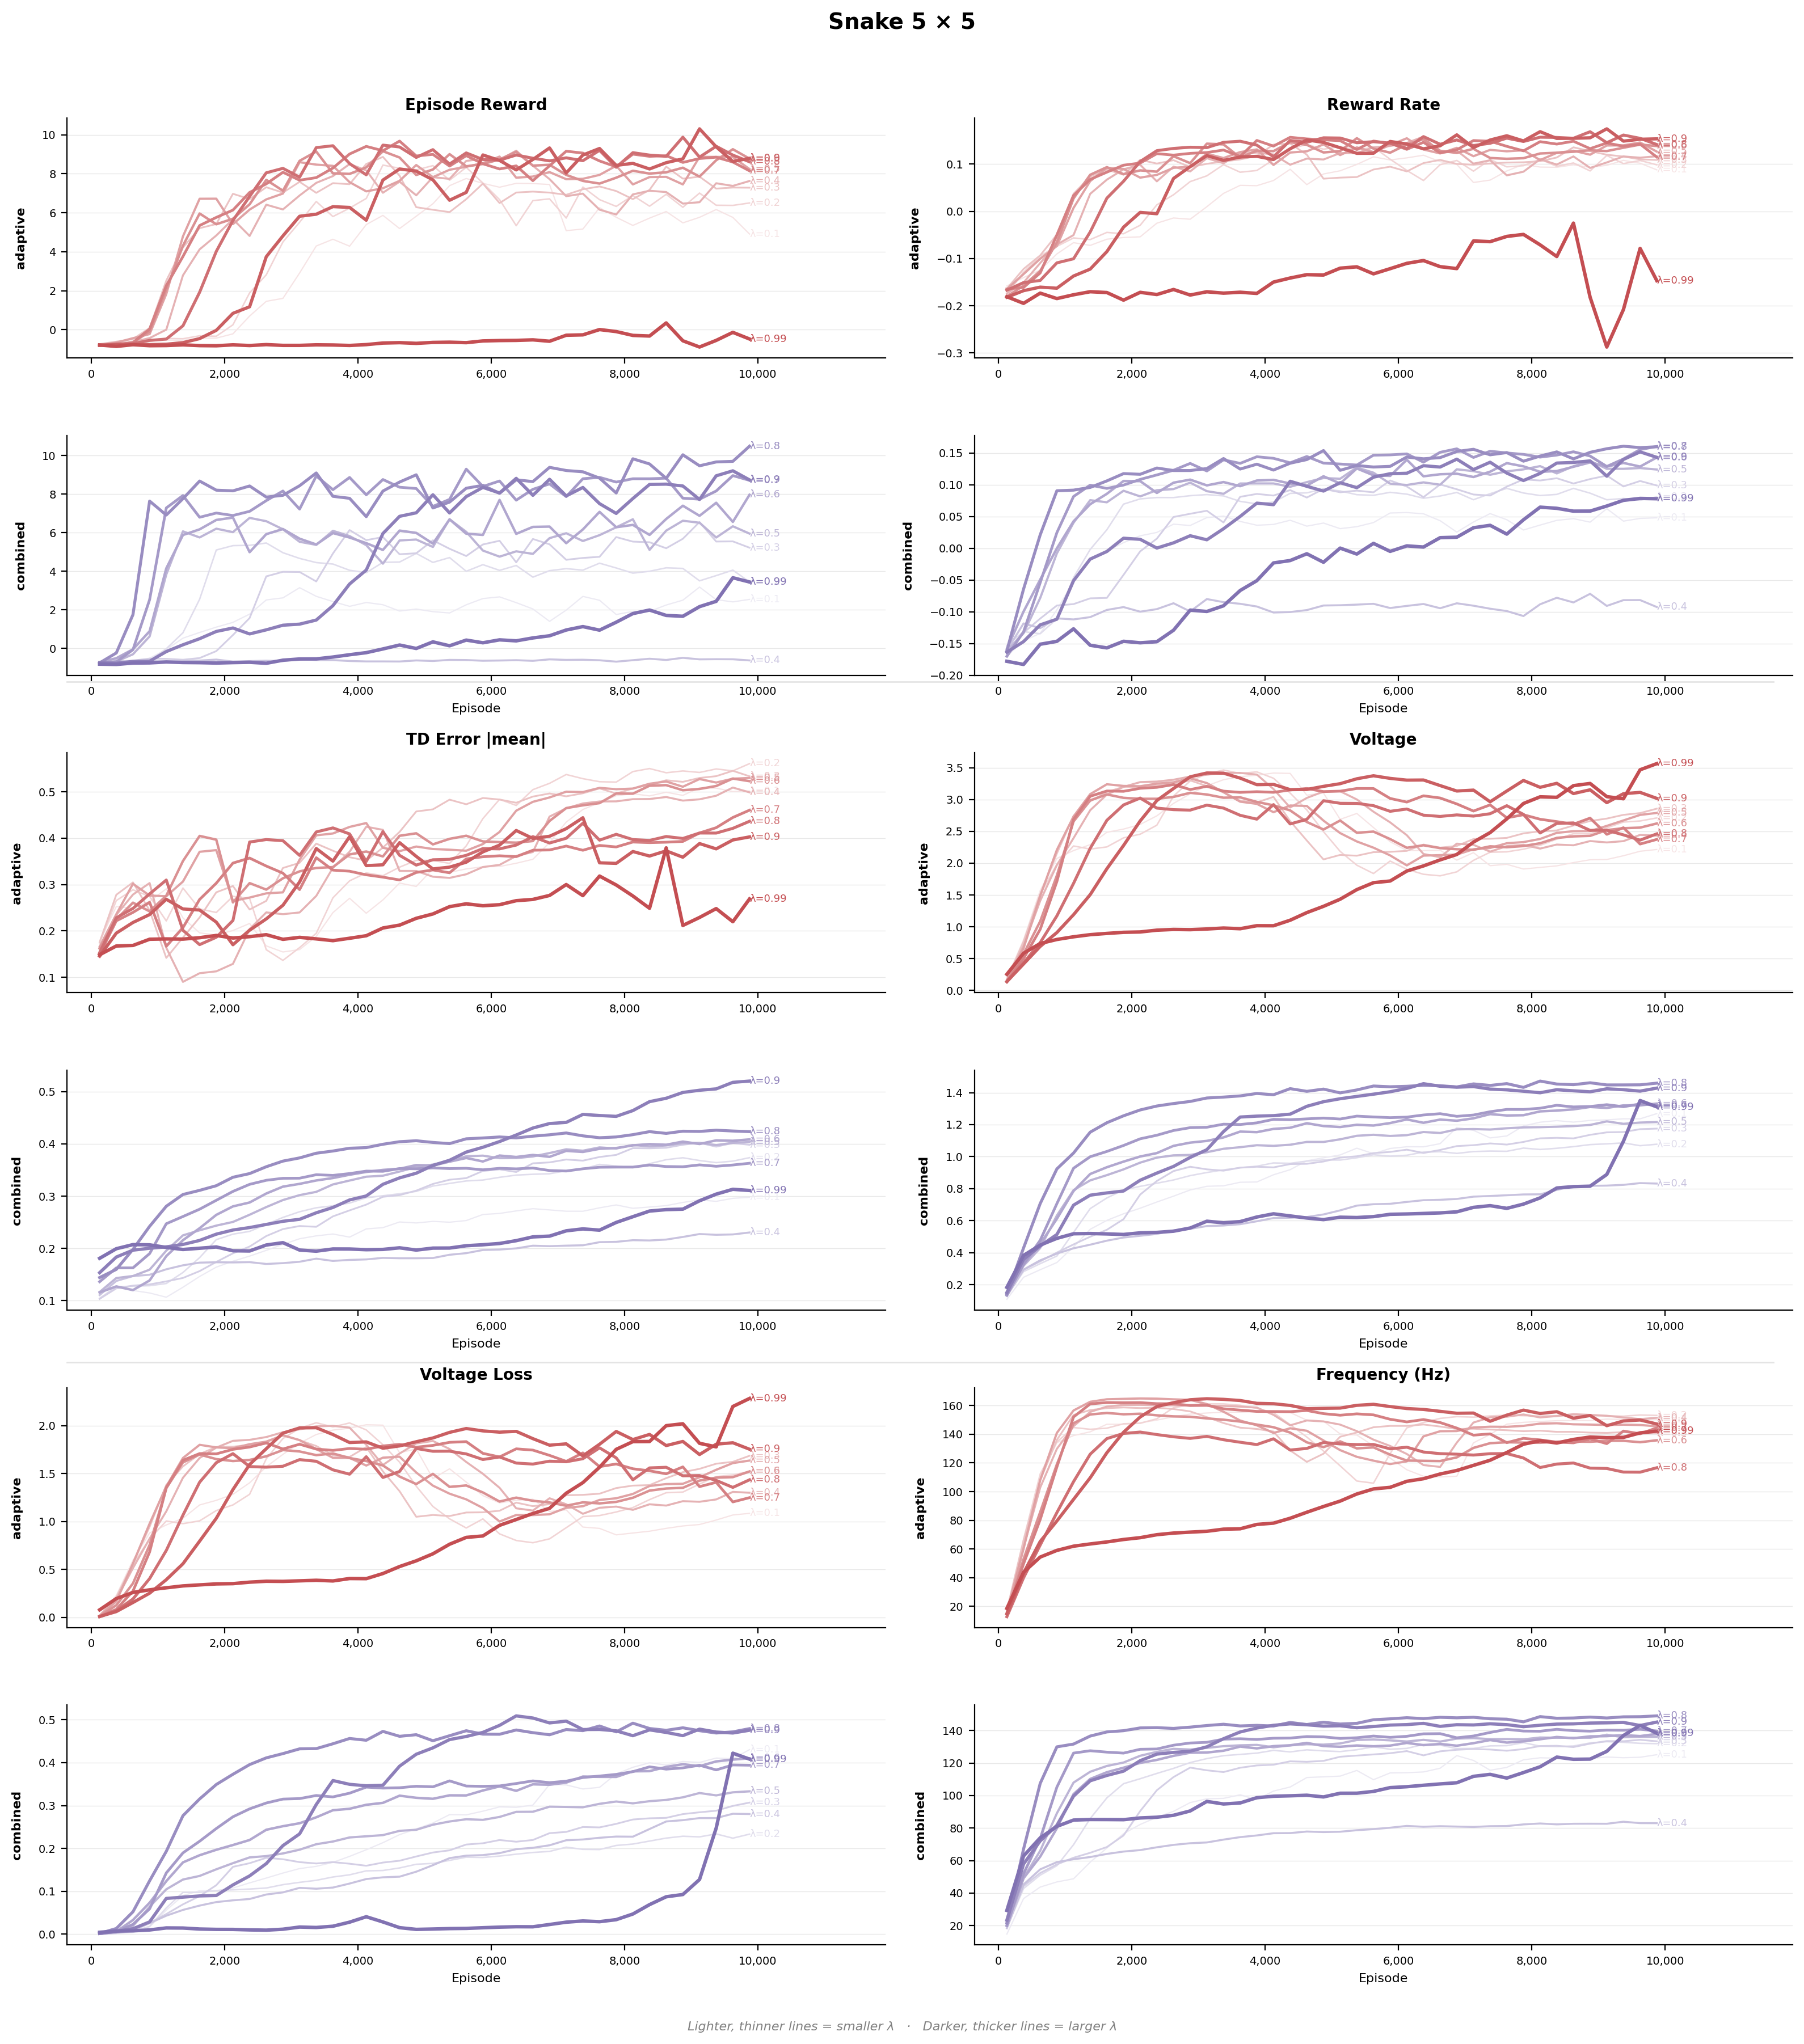
\includegraphics[width=\textwidth]{images/SnakeLambdaComparison.png}
    \caption[Lambda sweep on Snake $5\times5$]{Training performance across
    10,000 episodes on the Snake $5\times5$ task for adaptive e-prop (red)
    and the hybrid \emph{combined} variant (purple), across varying
    decay factors $\lambda \in \{0.1, 0.2, \ldots,
    0.9, 0.99\}$ (lighter, thinner lines correspond to smaller $\lambda$;
    darker, thicker lines to larger $\lambda$). Metrics reported include
    episode reward, reward rate, TD error (mean), voltage, voltage loss,
    and frequency (Hz).}
    \label{fig:snake_lambda}
\end{figure}

The distributed-family variant used for this sweep is \emph{combined}
instead of \emph{weight dist} or \emph{weight dist prop}. This
choice follows directly from the initial comparison in
Figure~\ref{fig:snake_comparison}, where \emph{combined} was
the strongest performer on Snake $5\times5$, reaching a high episode reward
faster than any other variant. Because we believe its update is dominated by the
synaptic perturbation term of \emph{weight dist} with the adaptively
routed feedback acting as a secondary contribution, we expect
\emph{combined} to behave similarly to \emph{weight dist} with respect
to $\lambda$, while benefiting from the additional stability that made it
the best-performing configuration in the initial experiment. We therefore
treat it here as a reasonable, and arguably more favorable, stand-in for
the perturbation-based family in this comparison.

On Snake, adaptive e-prop is remarkably robust to the choice of $\lambda$:
every value tested except $\lambda = 0.99$ converges to a comparable
episode reward in the range of 8 to 10, with only the speed of convergence
differing across the sweep, smaller $\lambda$ values take visibly longer to
rise but reach essentially the same plateau as the rest. Only the most
extreme value, $\lambda = 0.99$, fails to learn at all, remaining at a
slightly negative episode reward for the full $10,000$ episodes and showing
the same large, erratic swings in reward rate, voltage, and voltage loss
that elsewhere in this chapter have accompanied a destabilized critic. The
\emph{combined} variant is comparatively less uniform: most values of
$\lambda$ between 0.5 and 0.9 reach a similar high reward, but
$\lambda = 0.4$ fails to learn within the training budget, and
$\lambda = 0.99$ learns somewhat but only after a long initial period
of flat reward. The failure of $\lambda = 0.4$ is
worth treating with particular caution, since it sits in the middle of a
range that otherwise learns reliably, with $0.3$, $0.5$, and $0.6$ all
reaching the high-reward plateau on either side of it. Because each point
in this sweep is a single run, as noted
above, this is more plausibly read as an unlucky individual run, for
instance an unfavorable initialization or an early run of bad exploration
that the perturbation-based update never fully recovered from, than as
evidence that $\lambda = 0.4$ is itself a uniquely poor choice for
\emph{combined}. Stochastic learning rules of this kind can occasionally
fail to get off the ground even at a hyperparameter setting that is
otherwise unremarkable, and without repeated seeds at this specific value
we cannot distinguish that explanation from a genuine, reproducible
sensitivity to $\lambda = 0.4$.

As we will see in Section~\ref{sec:lambda_comparison}, this is the
opposite of the ordering observed on the Pac-Man randomized layouts
problem, where it is the distributed-style variant that tolerates a wide
range of $\lambda$ while adaptive e-prop shows an inconsistent and often
delayed learning onset. Here, on Snake, it is adaptive e-prop that appears
to be the more forgiving of the two with respect to $\lambda$, with only
the single extreme value $\lambda = 0.99$ causing outright failure, while
\emph{combined} shows a less monotonic and somewhat narrower band of
$\lambda$ values for which it learns promptly. Taken together, the two
experiments will support the broader argument of this chapter: 
neither structured feedback-based credit assignment nor
perturbation-based credit assignment is uniformly more robust to the
decay factor $\lambda$. Which rule tolerates a wider or more reliable
range of $\lambda$ appears to depend on the task, and possibly on other
interacting factors such as architecture depth or reward sparsity that
differ between Snake and Pac-Man, and not an intrinsic property
of either algorithm.

\subsection{Depth Comparison}
\label{subsec:snake-depth-comparison}

\begin{figure}[htpb]
    \centering
    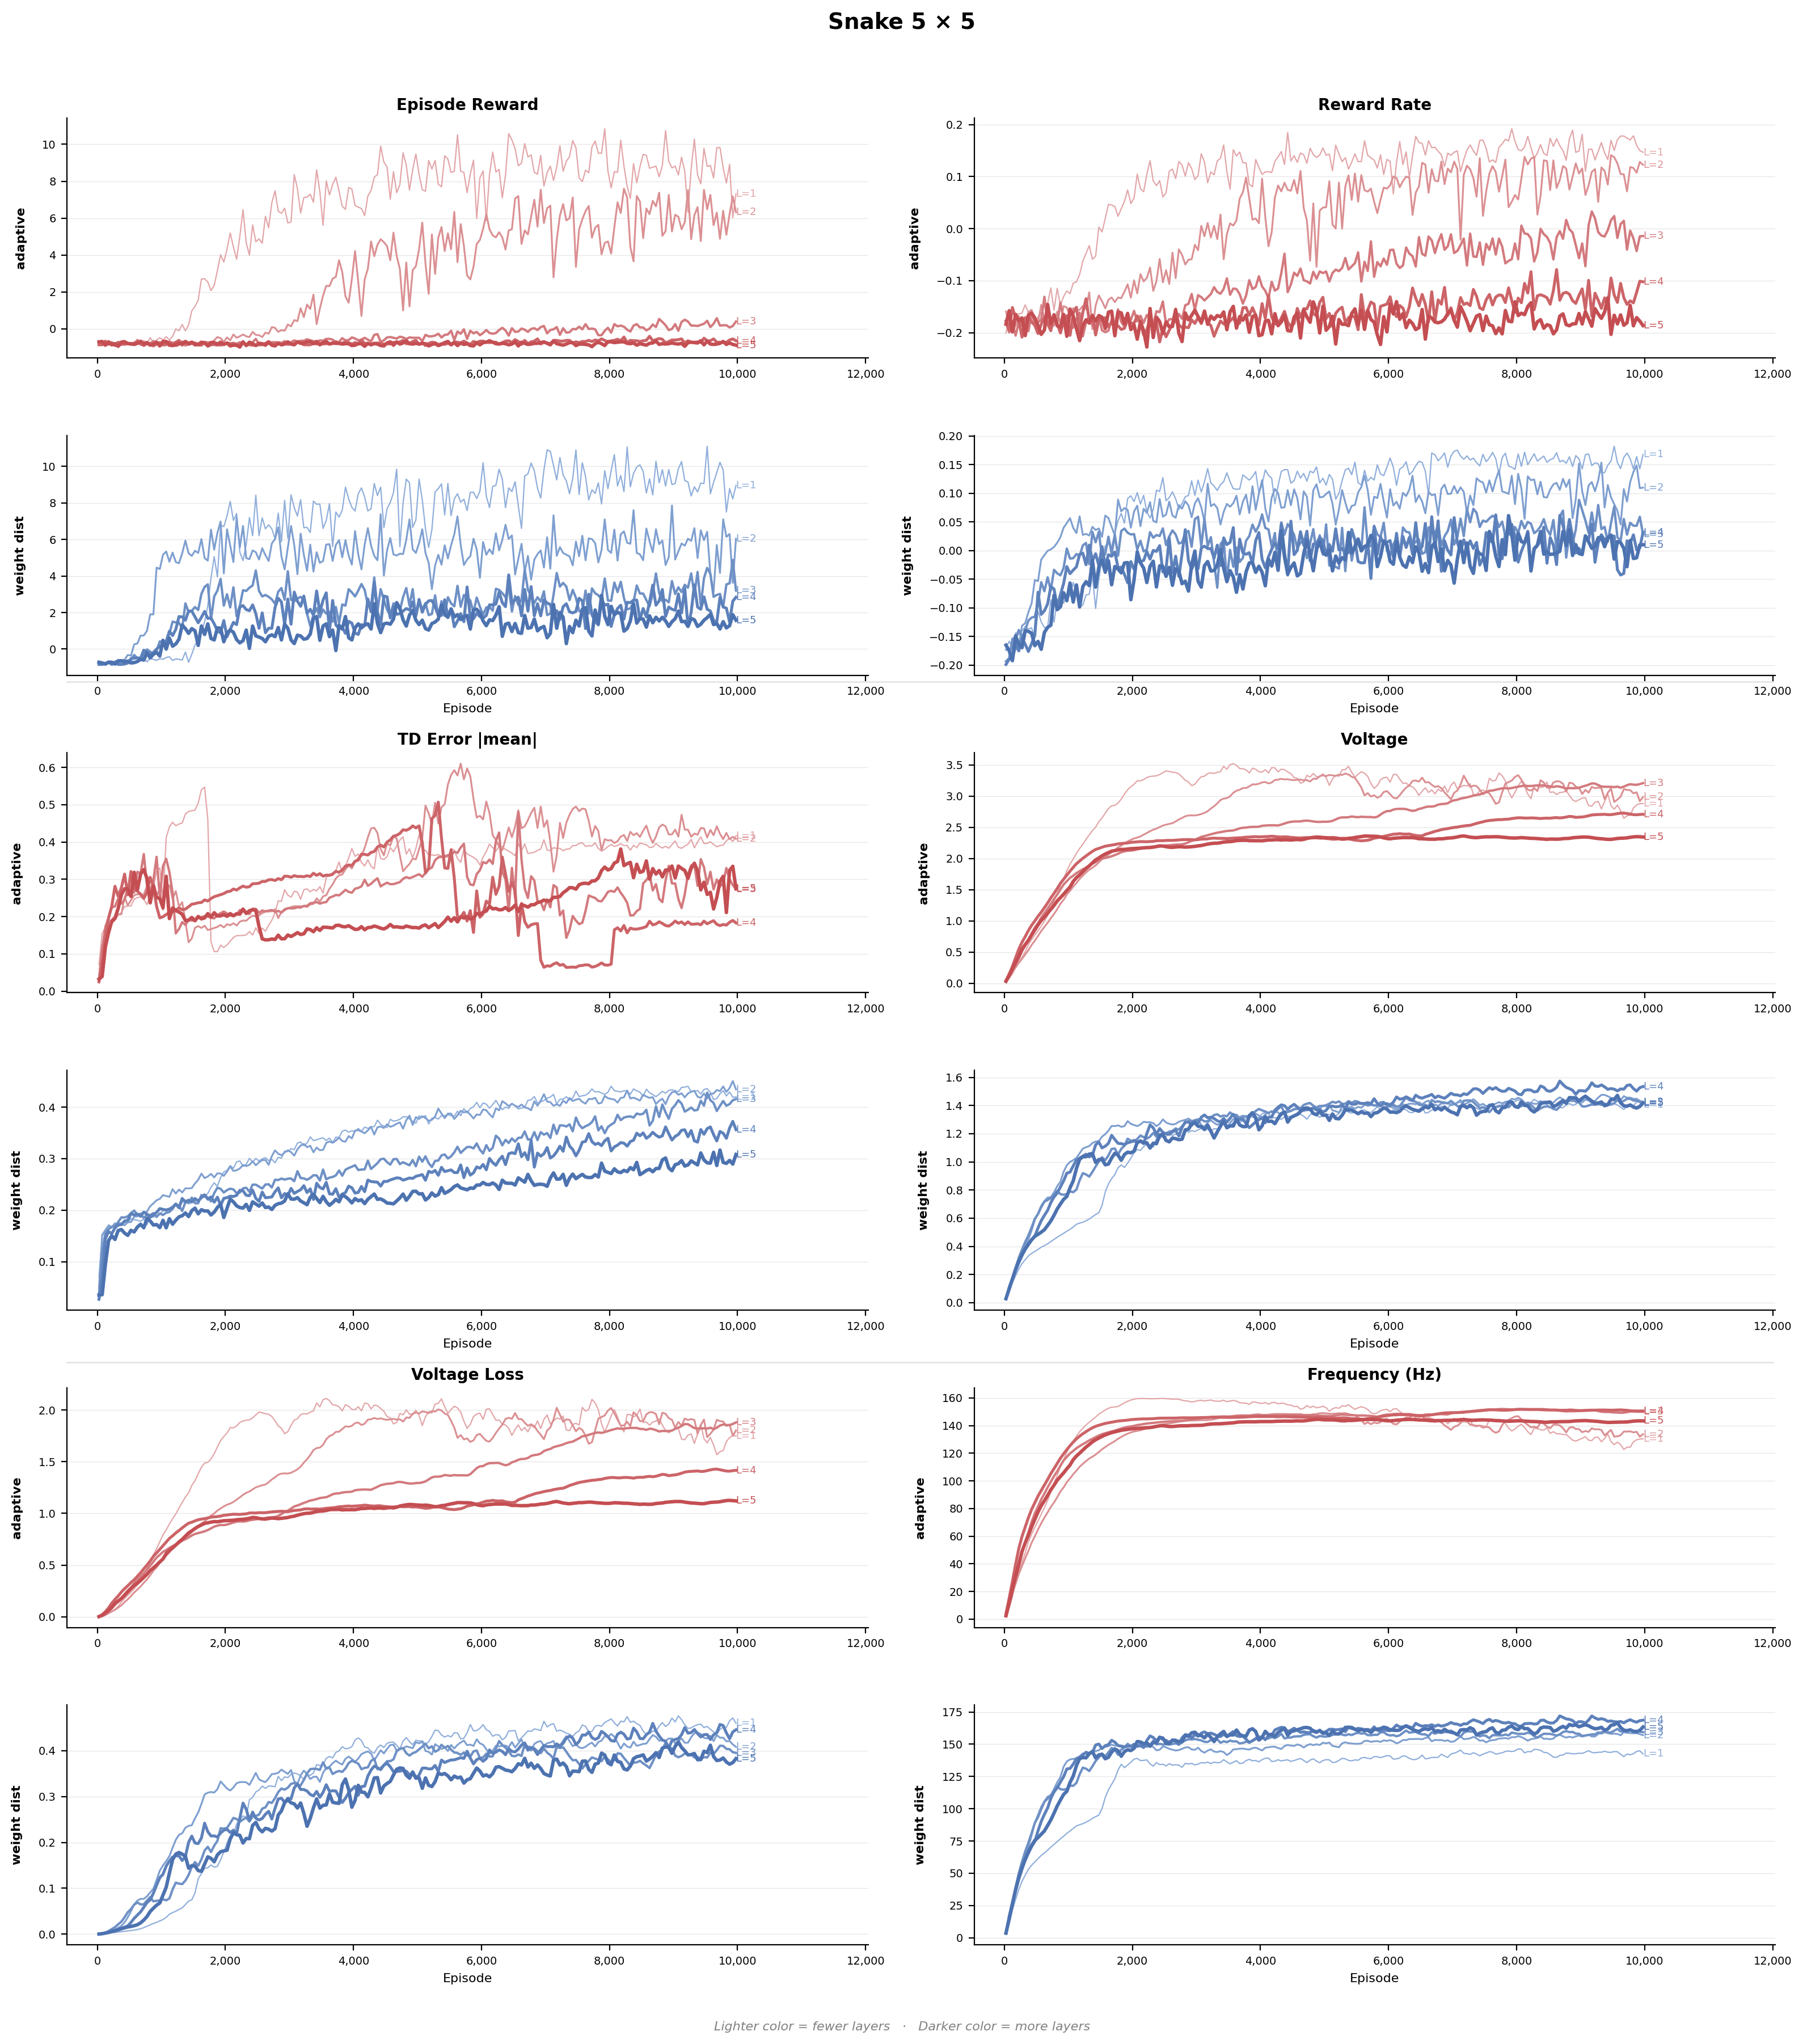
\includegraphics[width=1.0\linewidth]{images/SnakeLayersComparison.png}
    \caption[Effect of network depth on Snake $5\times5$]{Effect of network depth on the Snake $5\times5$ task, comparing adaptive e-prop
    (red, upper sub-row of each metric) and distributed e-prop (\emph{weight dist}, blue, lower
    sub-row) across networks with different numbers of layers. Colour shade encodes depth: lighter
    shades correspond to shallower networks and darker shades to deeper ones. Each panel reports
    one of the six standard metrics (episode reward, reward rate, mean absolute TD error, voltage,
    voltage loss, and frequency in Hz) over $10{,}000$ episodes. Increasing depth lengthens the
    causal path between input and output, and the figure shows how the learning of each rule
    degrades as that path grows.}
    \label{fig:snake-depth-comparison}
\end{figure}

Figure~\ref{fig:snake-depth-comparison} reports the six standard metrics for both rules across
networks of increasing depth, with lighter shades denoting shallower networks and darker shades
deeper ones. In
the episode reward and reward rate panels, both rules display a clear ordering by depth where the
shallowest networks reach the highest reward and reward rate, and the curves fall steadily as
layers are added. The rules differ in how pronounced this decline is. For adaptive e-prop the
spread across depths is wide: the shallowest network reaches a reward of roughly eight to ten,
while the deepest networks stay close to zero for the full $10{,}000$ episodes. For distributed
e-prop the spread is narrower: the shallowest network reaches a comparable reward, and although
the deeper networks again score lower, every depth tested converges to a clearly positive
reward. The reward rate panels follow the same pattern, with the deepest adaptive networks
settling at negative values and the deepest distributed networks remaining near zero or above.

The remaining panels describe the value-error and spiking dynamics. In the TD error panels,
both rules show an error that grows over training and increases with depth, with the adaptive
curves visibly noisier and reaching larger values while the distributed curves grow more
smoothly. The voltage and voltage-loss panels show a consistent gap between the rules, we have that adaptive
e-prop reaches a higher membrane voltage, around three, and a higher voltage loss, both rising
with depth, whereas distributed e-prop holds a lower and flatter voltage, around one and a half,
together with a small voltage loss across all depths. The firing frequency converges to a
similar high band of roughly $140$ to $170$ Hz for both rules at every depth, separating the
configurations only marginally.

The depth comparison above invites a tempting but, we believe, mistaken conclusion: that
distributed e-prop is intrinsically better suited to longer causal paths. Because we knew from the
outset that e-prop with aligned feedback can be slow to start, learning only once its feedback
pathway and internal dynamics have settled into agreement, we ran a deeper configuration for a
much longer horizon to test this directly. We do so under two update schemes for a five-layer
network on Snake $5\times5$: Figure~\ref{fig:snake-extended-perstep} applies the weight update
continuously, once per environment step, while Figure~\ref{fig:snake-extended-perepisode} applies
it once per episode. Both span roughly $100{,}000$ episodes.

The extended runs reverse the impression left by the fixed-budget comparison, and they do so under
both update schemes. The distributed variants behave exactly as before: they reach a usable reward
within the first few thousand episodes and then stop improving, holding that plateau for the rest
of training, whether the weight update is applied continuously (Figure~\ref{fig:snake-extended-perstep})
or once per episode, where the \emph{combined} variant behaves much like \emph{weight dist}
(Figure~\ref{fig:snake-extended-perepisode}). Adaptive e-prop, by contrast, spends a long initial
phase near zero reward, the signature of feedback alignment that has not yet taken effect, and only
then begins to learn. Once it does, it continues to improve past the level at which the distributed
variants stalled, and is still improving when each run ends. The spiking-dynamics panels tell the
same story in both figures: adaptive e-prop operates at a markedly higher membrane voltage and
voltage loss, rising during its learning phase, while the distributed variants stay low and flat,
and the firing frequencies remain in a similar high band with adaptive e-prop running slightly lower.

We read this as a caution, and even then only provisionally. The
deep-network collapse of adaptive e-prop in the depth comparison is not evidence that the rule
cannot handle longer causal paths; in this case, it appears to be an artifact of the training
budget, since the same configuration begins to learn the task when given more time. What seems
to distinguish the two rules here is less their capability than their dynamics: distributed
e-prop tends to find a reasonable solution quickly and then improve little further, while
adaptive e-prop is slow to start, plausibly because feedback alignment takes time, without
showing clear signs of being fundamentally limited by depth. These remain possibilities, 
because the hyperparameters have not been tuned exhaustively, and a given
setting can favor one rule while handicapping the other, any apparent advantage may reflect the
particular configuration tested rather than a property of the algorithm itself. We therefore do
not claim that either rule is better at handling causal path length, and present this longer run
only as an example of why the immediate interpretation of the depth comparison cannot be taken
at face value.

\begin{figure}[H]
    \centering
    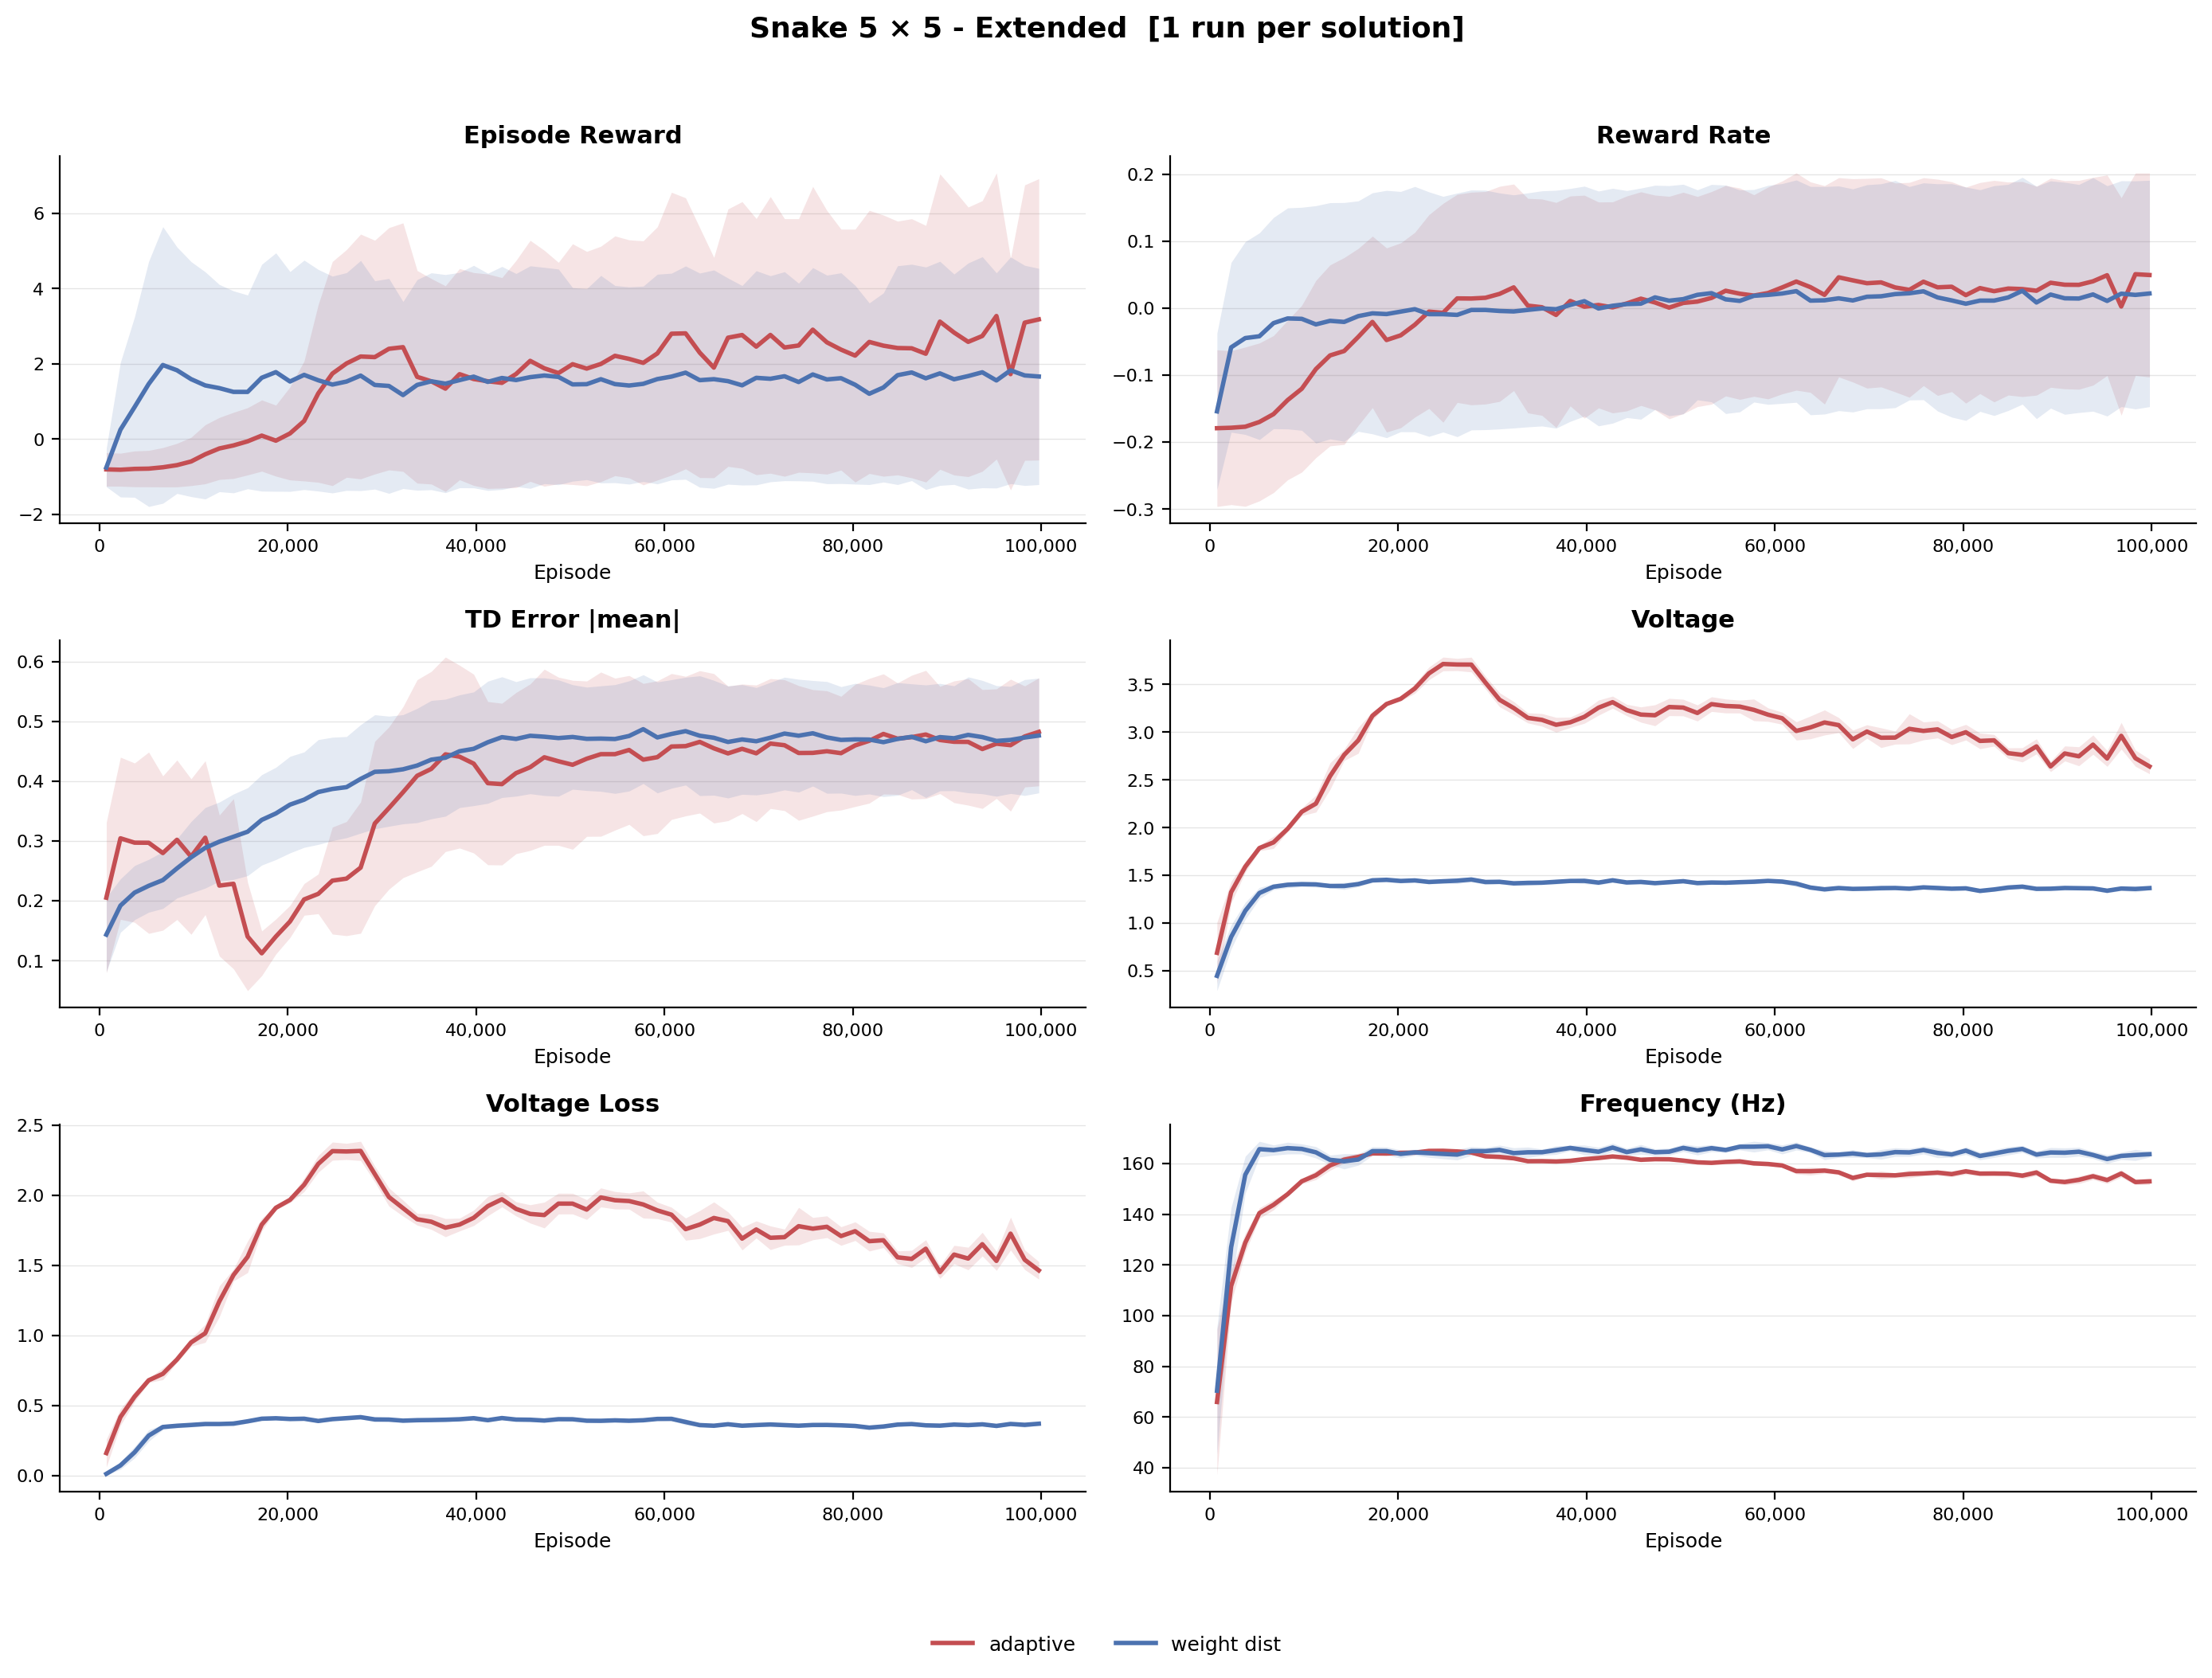
\includegraphics[width=1\linewidth]{images/comparison_extended_1_runs.png}
    \caption[Extended training, 5-layer network, updates per step (Snake)]{Extended,
    longer-horizon training on Snake $5\times5$ with a five-layer network, comparing adaptive
    e-prop (red) with distributed e-prop (\emph{weight dist}, blue) when the weight update is
    applied continuously, once per environment step. One run per configuration; the six standard
    metrics are shown over roughly $100{,}000$ episodes. Distributed e-prop converges within the
    first few thousand episodes and then holds a plateau, whereas adaptive e-prop makes little
    progress for an extended initial period before beginning to learn and overtaking it.}
    \label{fig:snake-extended-perstep}
\end{figure}

Comparing the two update schemes is itself informative. The per-episode updates were clearly
beneficial for both rules, adaptive e-prop and \emph{weight dist} each reach a higher episode
reward and reward rate under per-episode updating (Figure~\ref{fig:snake-extended-perepisode})
than under the continuous, per-step scheme (Figure~\ref{fig:snake-extended-perstep}). The
\emph{combined} variant, by contrast, was consistently the weakest of the three across the
performance metrics. This is genuinely surprising, since in the single-layer comparison of all
rules on this same task (Figure~\ref{fig:snake_comparison}) combined e-prop was among the
better-performing variants; the deeper, longer-horizon setting evidently reverses that standing.

\begin{figure}[H]
    \centering
    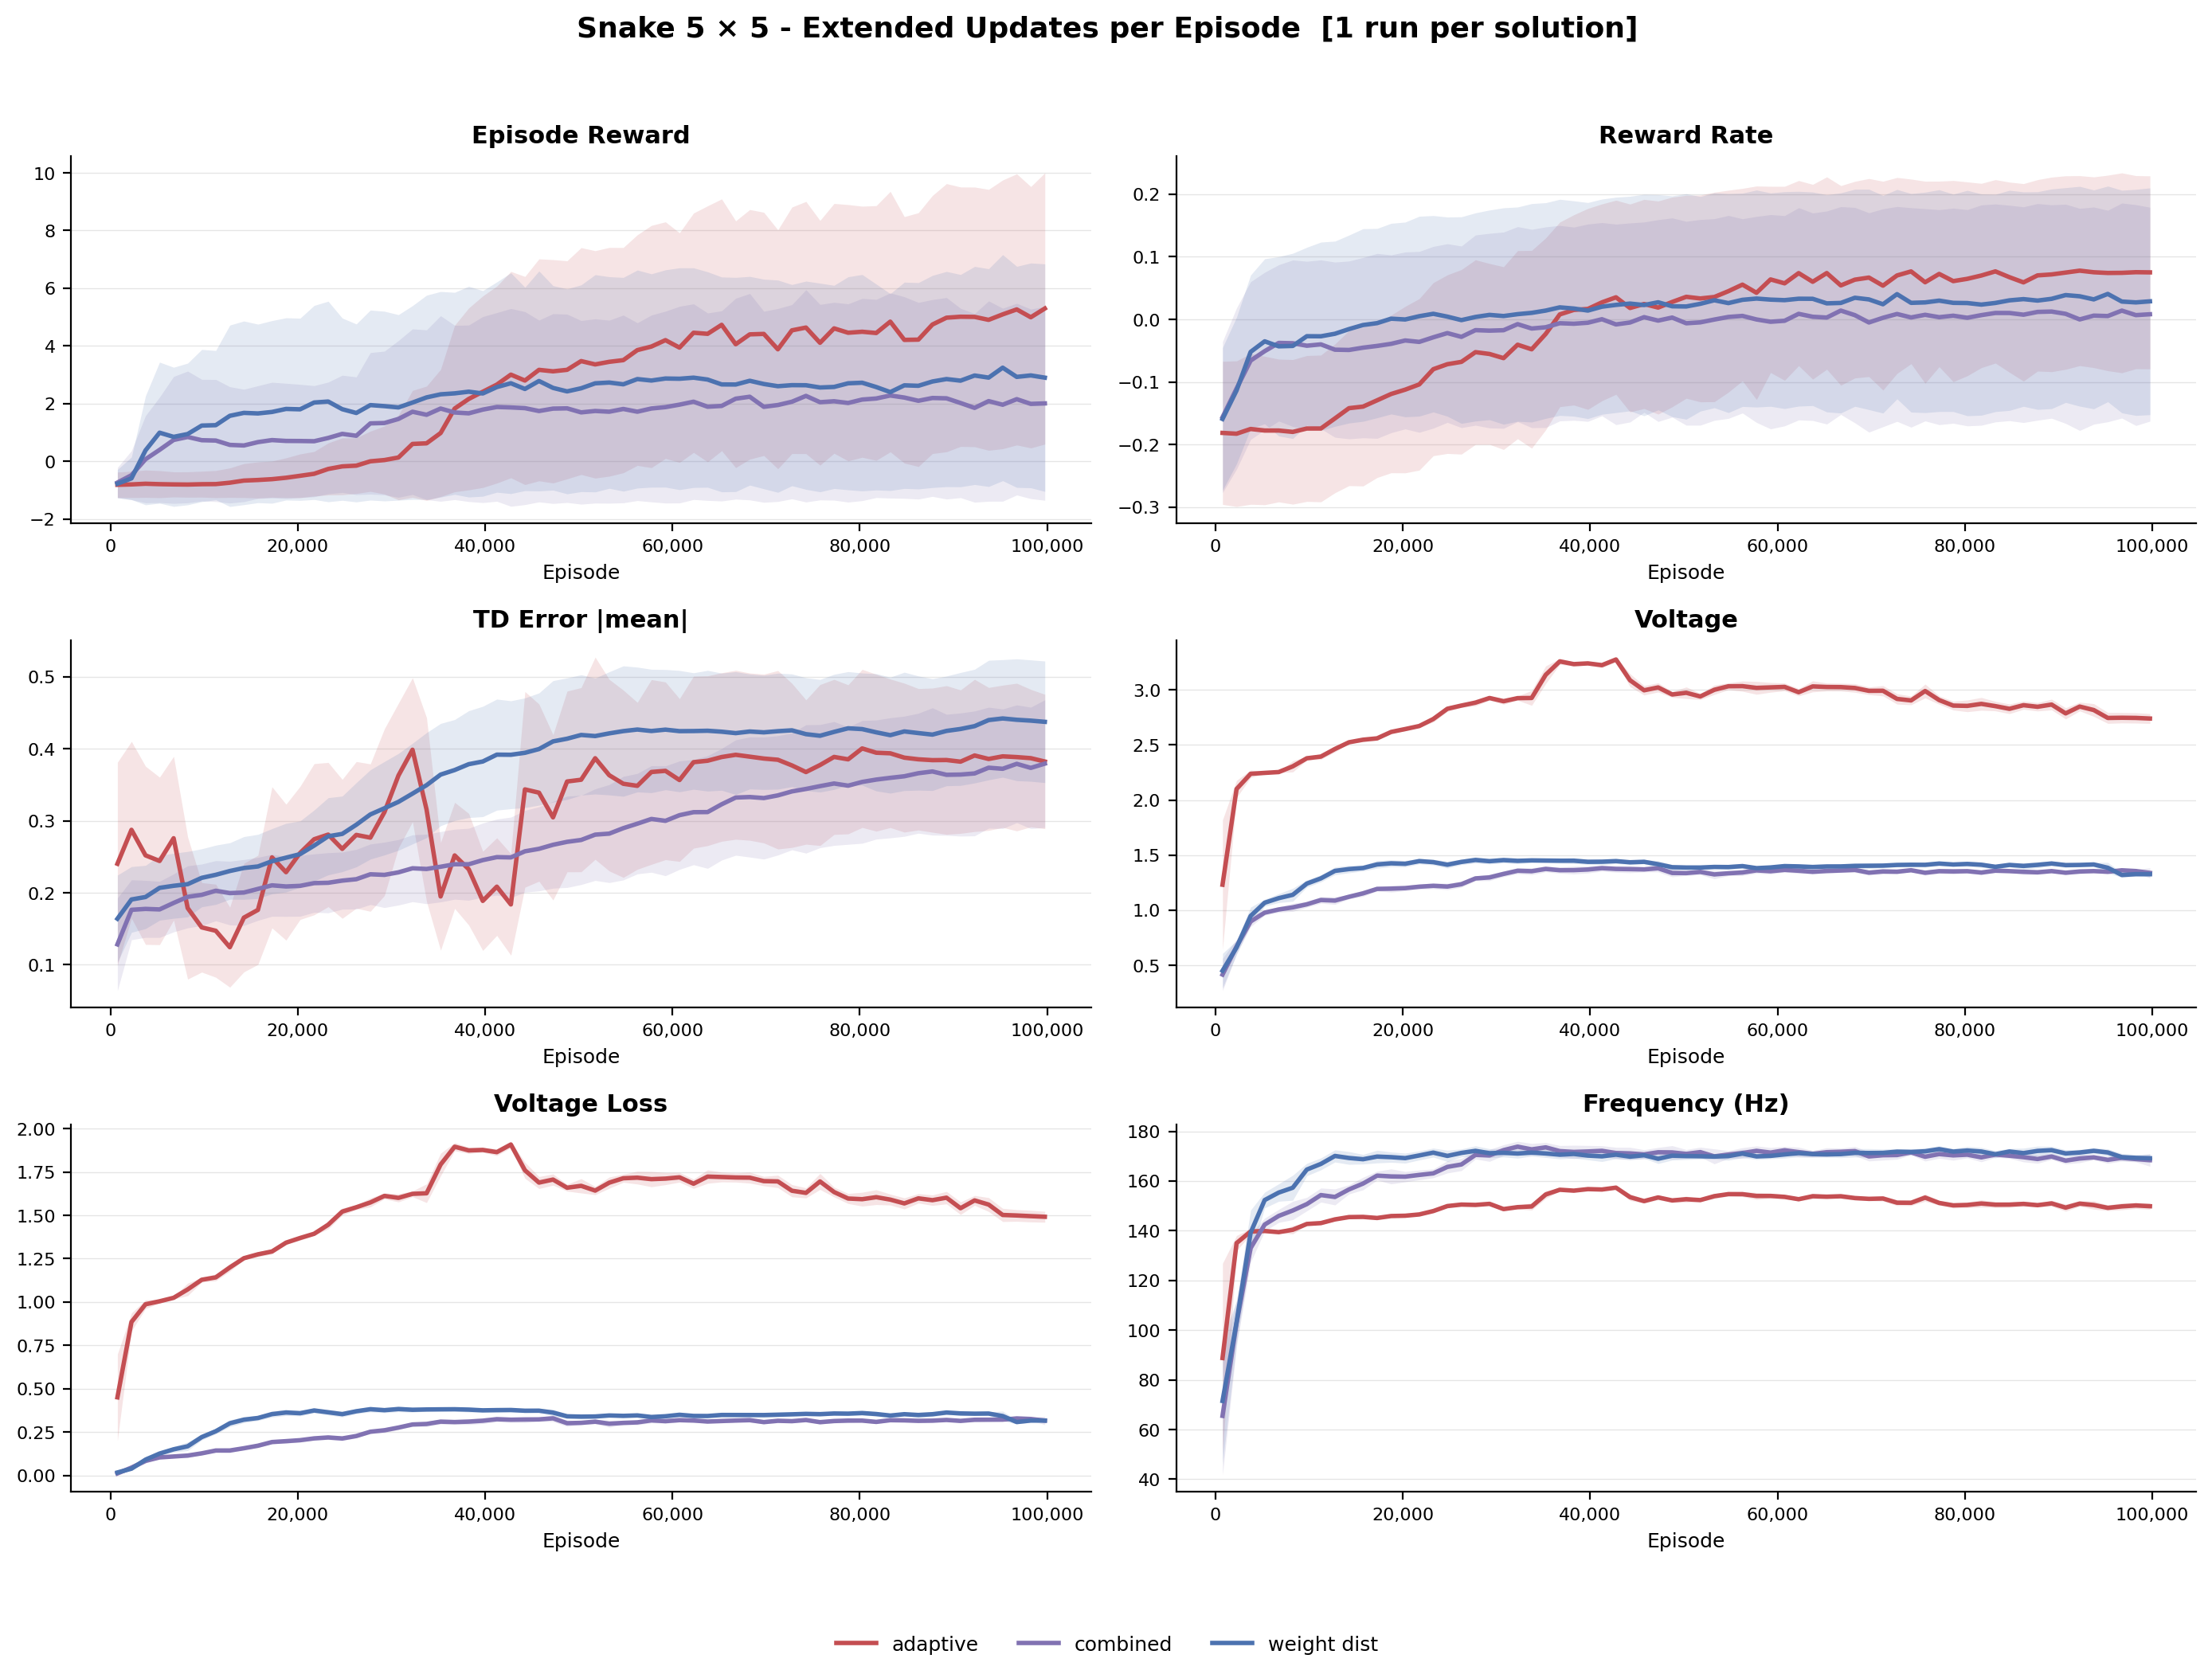
\includegraphics[width=1\linewidth]{images/comparison_extended_updates_per_episode_1_runs.png}
    \caption[Extended training, 5-layer network, updates per episode (Snake)]{The same extended
    setup as Figure~\ref{fig:snake-extended-perstep}, but with the weight update applied once per
    episode. Adaptive e-prop (red) is compared with two distributed
    variants, \emph{weight dist} (blue) and \emph{combined} (purple). One run per configuration;
    the six standard metrics over roughly $100{,}000$ episodes. The qualitative pattern is
    unchanged: the distributed variants plateau early while adaptive e-prop starts slowly and then
    continues to improve past them.}
    \label{fig:snake-extended-perepisode}
\end{figure}

Figure~\ref{fig:snake-qualitative-depth} provides a qualitative look inside
a single representative episode for \emph{weight dist} at two different
network depths. The 2-layer network produces a value estimate with clear
predictive structure, rising ahead of reward events and falling ahead of
penalties, while the 5-layer network develops a comparatively flat and
unstructured estimate that fails to anticipate upcoming events. The action
probability show a possible failure reason, the shallower network retains
a more distributed policy with intermediate probability mass across multiple
actions, whereas the deeper network collapses to a near-deterministic policy
at almost every timestep, which limits exploration and therefore learning. 
Both observations are consistent with the
performance plateau seen in Figures
~\ref{fig:snake-extended-perstep}, ~\ref{fig:snake-extended-perepisode} and ~\ref{fig:snake-depth-comparison}, though whether
the observations are a cause or a consequence 
is difficult to establish from these results alone.

\begin{figure}[H]
    \centering
    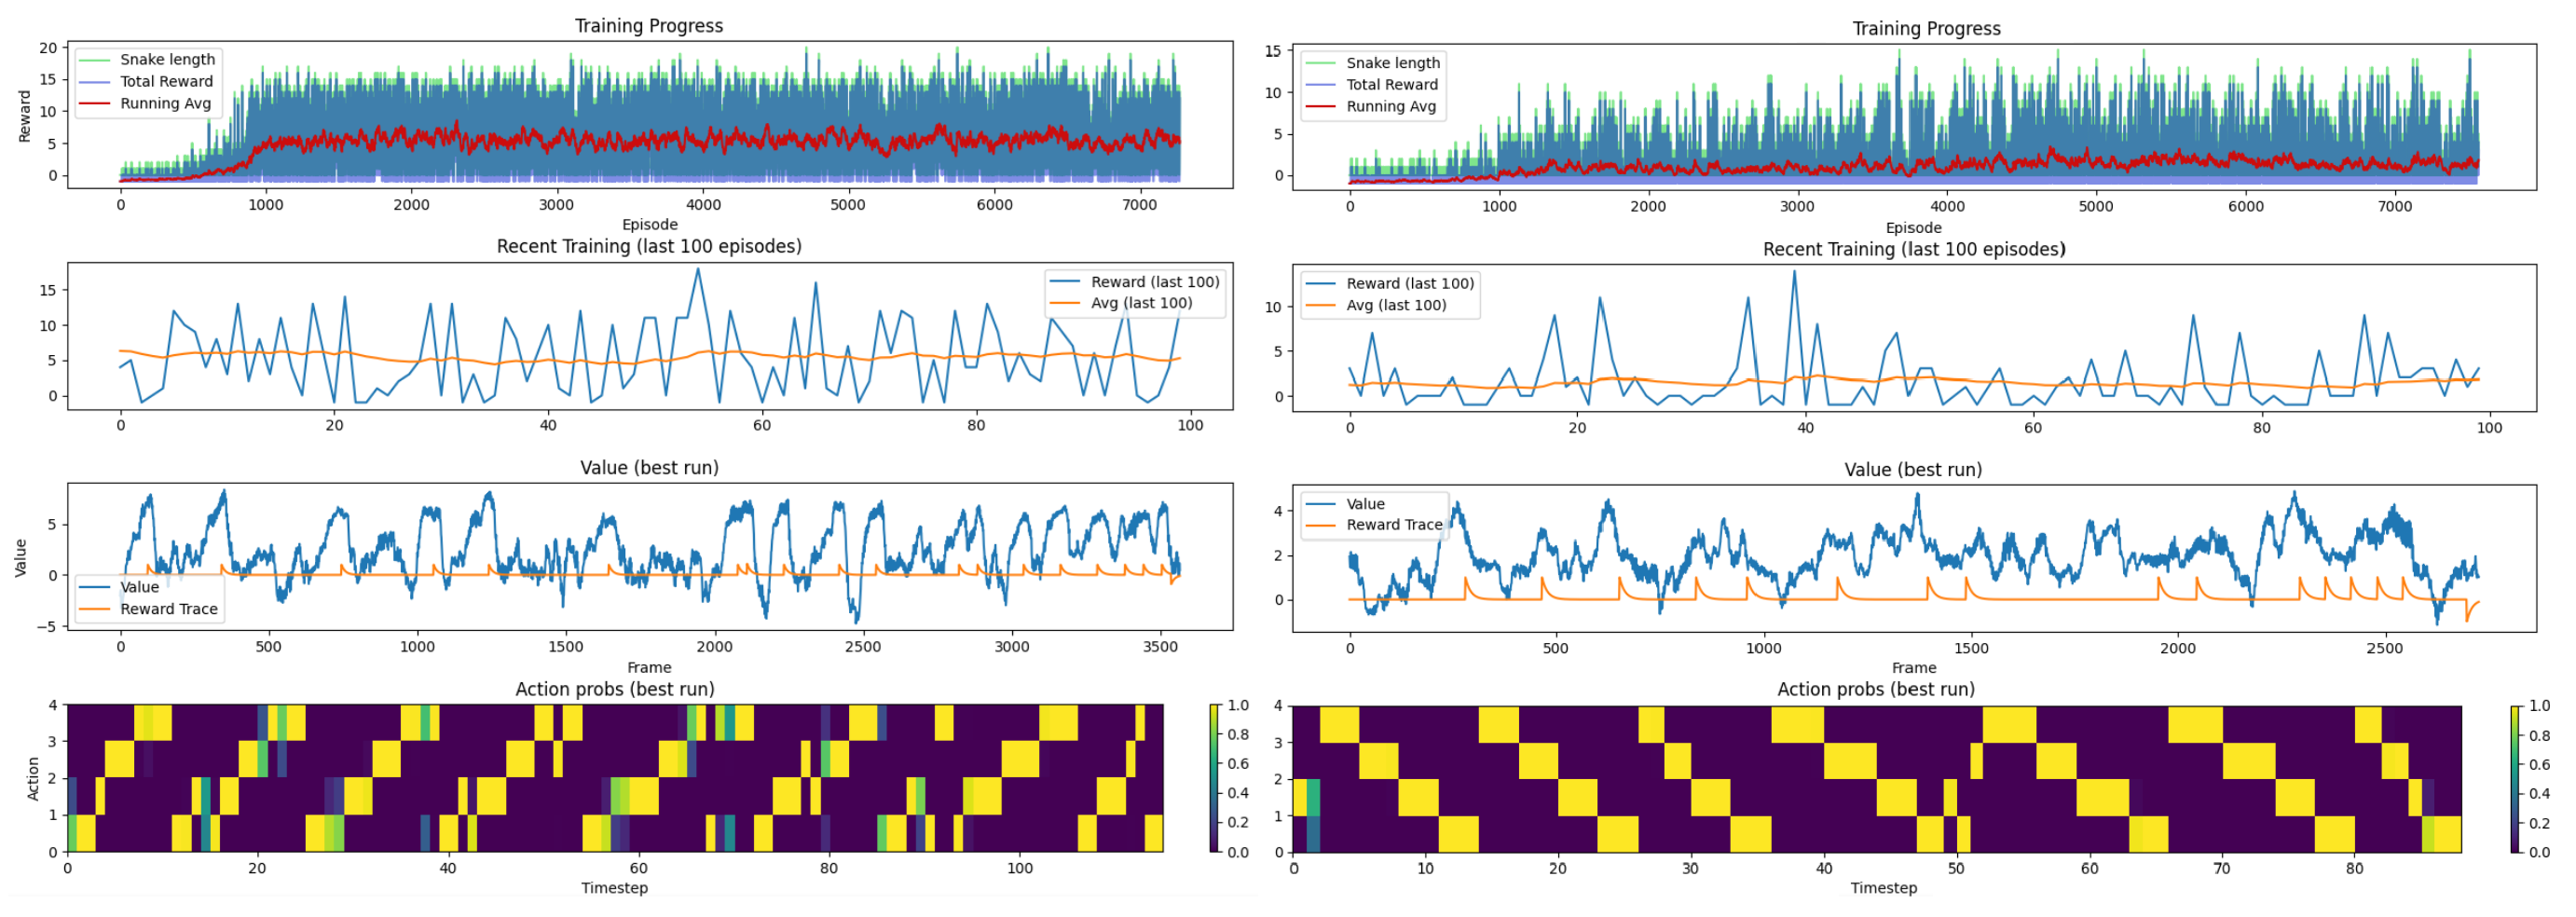
\includegraphics[width=1\linewidth]{images/SnakeQualitative2vs5Layers.png}
    \caption[Qualitative \emph{weight dist}, depth comparison]{Qualitative comparison of \emph{weight dist} on Snake
    $5 \times 5$ at two network depths. Each column shows a representative
    episode from a 2-layer (left) and 5-layer (right) network at a similar
    stage of training. From top to bottom: training progress over all episodes;
    reward over the most recent 100 episodes against its running mean; the value
    estimate $V_t$ against the reward trace; and a heatmap of the action
    probabilities through the episode.}
    \label{fig:snake-qualitative-depth}
\end{figure}

\subsection{Reward-based regularization Exploration}
\label{sec:regularization-exploration}

Figure~\ref{fig:snake-regularization} explores the effect of the
reward-based regularization terms introduced in
Section~\ref{subsec:regularization} on the \emph{weight dist}
variant on Snake $5 \times 5$, sweeping over the regularization strength
$c_{reg}$. Two broad trends are visible across the metrics. First,
increasing regularization strength consistently reduces task performance,
suggesting that beyond a certain point the regularization signal competes
with the task reward signal for control of the perturbation traces, pulling
weight updates away from task-relevant directions. Second, the two
regularization targets, voltage and firing frequency, respond differently
to the same regularization pressure.

Voltage regularization appears to be the easier objective for the network
to satisfy: the voltage metrics respond clearly and consistently to
increasing $c_{reg}$, with membrane potentials brought closer to a
well-regulated range even at moderate regularization strengths. A plausible
explanation for why this works so well in the distributed e-prop framework
is that voltage deviation is an entirely local quantity, observable at the
level of a single neuron without any reference to the global network state.
This makes it a natural fit for the perturbation-based update rule, where
each neuron acts as an independent stochastic actor: the local voltage
reward provides a local evaluative signal that is directly compatible with
the local perturbation traces, without requiring any credit to be routed
across the network. This observation opens an interesting direction for
future work, namely the design of other local reward signals that exploit
this compatibility more deliberately, potentially allowing neurons to
optimize local objectives that complement the global task reward in ways
that structured feedback rules cannot easily support.

Frequency regularization proves harder to enforce, with only a modest effect
visible even at larger values of $c_{reg}$. The reasons for this are not
entirely clear, and we do not attempt to offer a definitive explanation here.

It is worth noting that we were unable to make voltage regularization work
within the standard e-prop framework. Although the exact cause remains
unclear, a likely contributing factor is that the standard e-prop voltage
regularization update depends directly on the presynaptic spike train and
adaptive threshold, and has no mechanism to suppress itself when the membrane
is in a pathological regime. The perturbation trace, by contrast, naturally
carries little signal when the membrane is far from threshold, since the
perturbations are unlikely to have influenced the spike output in that
regime, which effectively gates the regularization update and prevents it
from generating runaway effects. The standard e-prop update lacks this
self-suppression, and may therefore produce large and poorly directed weight
changes precisely when the membrane dynamics are most unstable, reinforcing
the pathology. Whether a modified formulation that
incorporates a similar gating mechanism could recover comparable behavior
remains an open question.

Surprisingly the best performance seen until now is given by the non 
regularized run with $c_{reg}=0.0$ as it can be seen in ~\ref{tab:snake-best100-score}.

\begin{figure}[H]
    \centering
    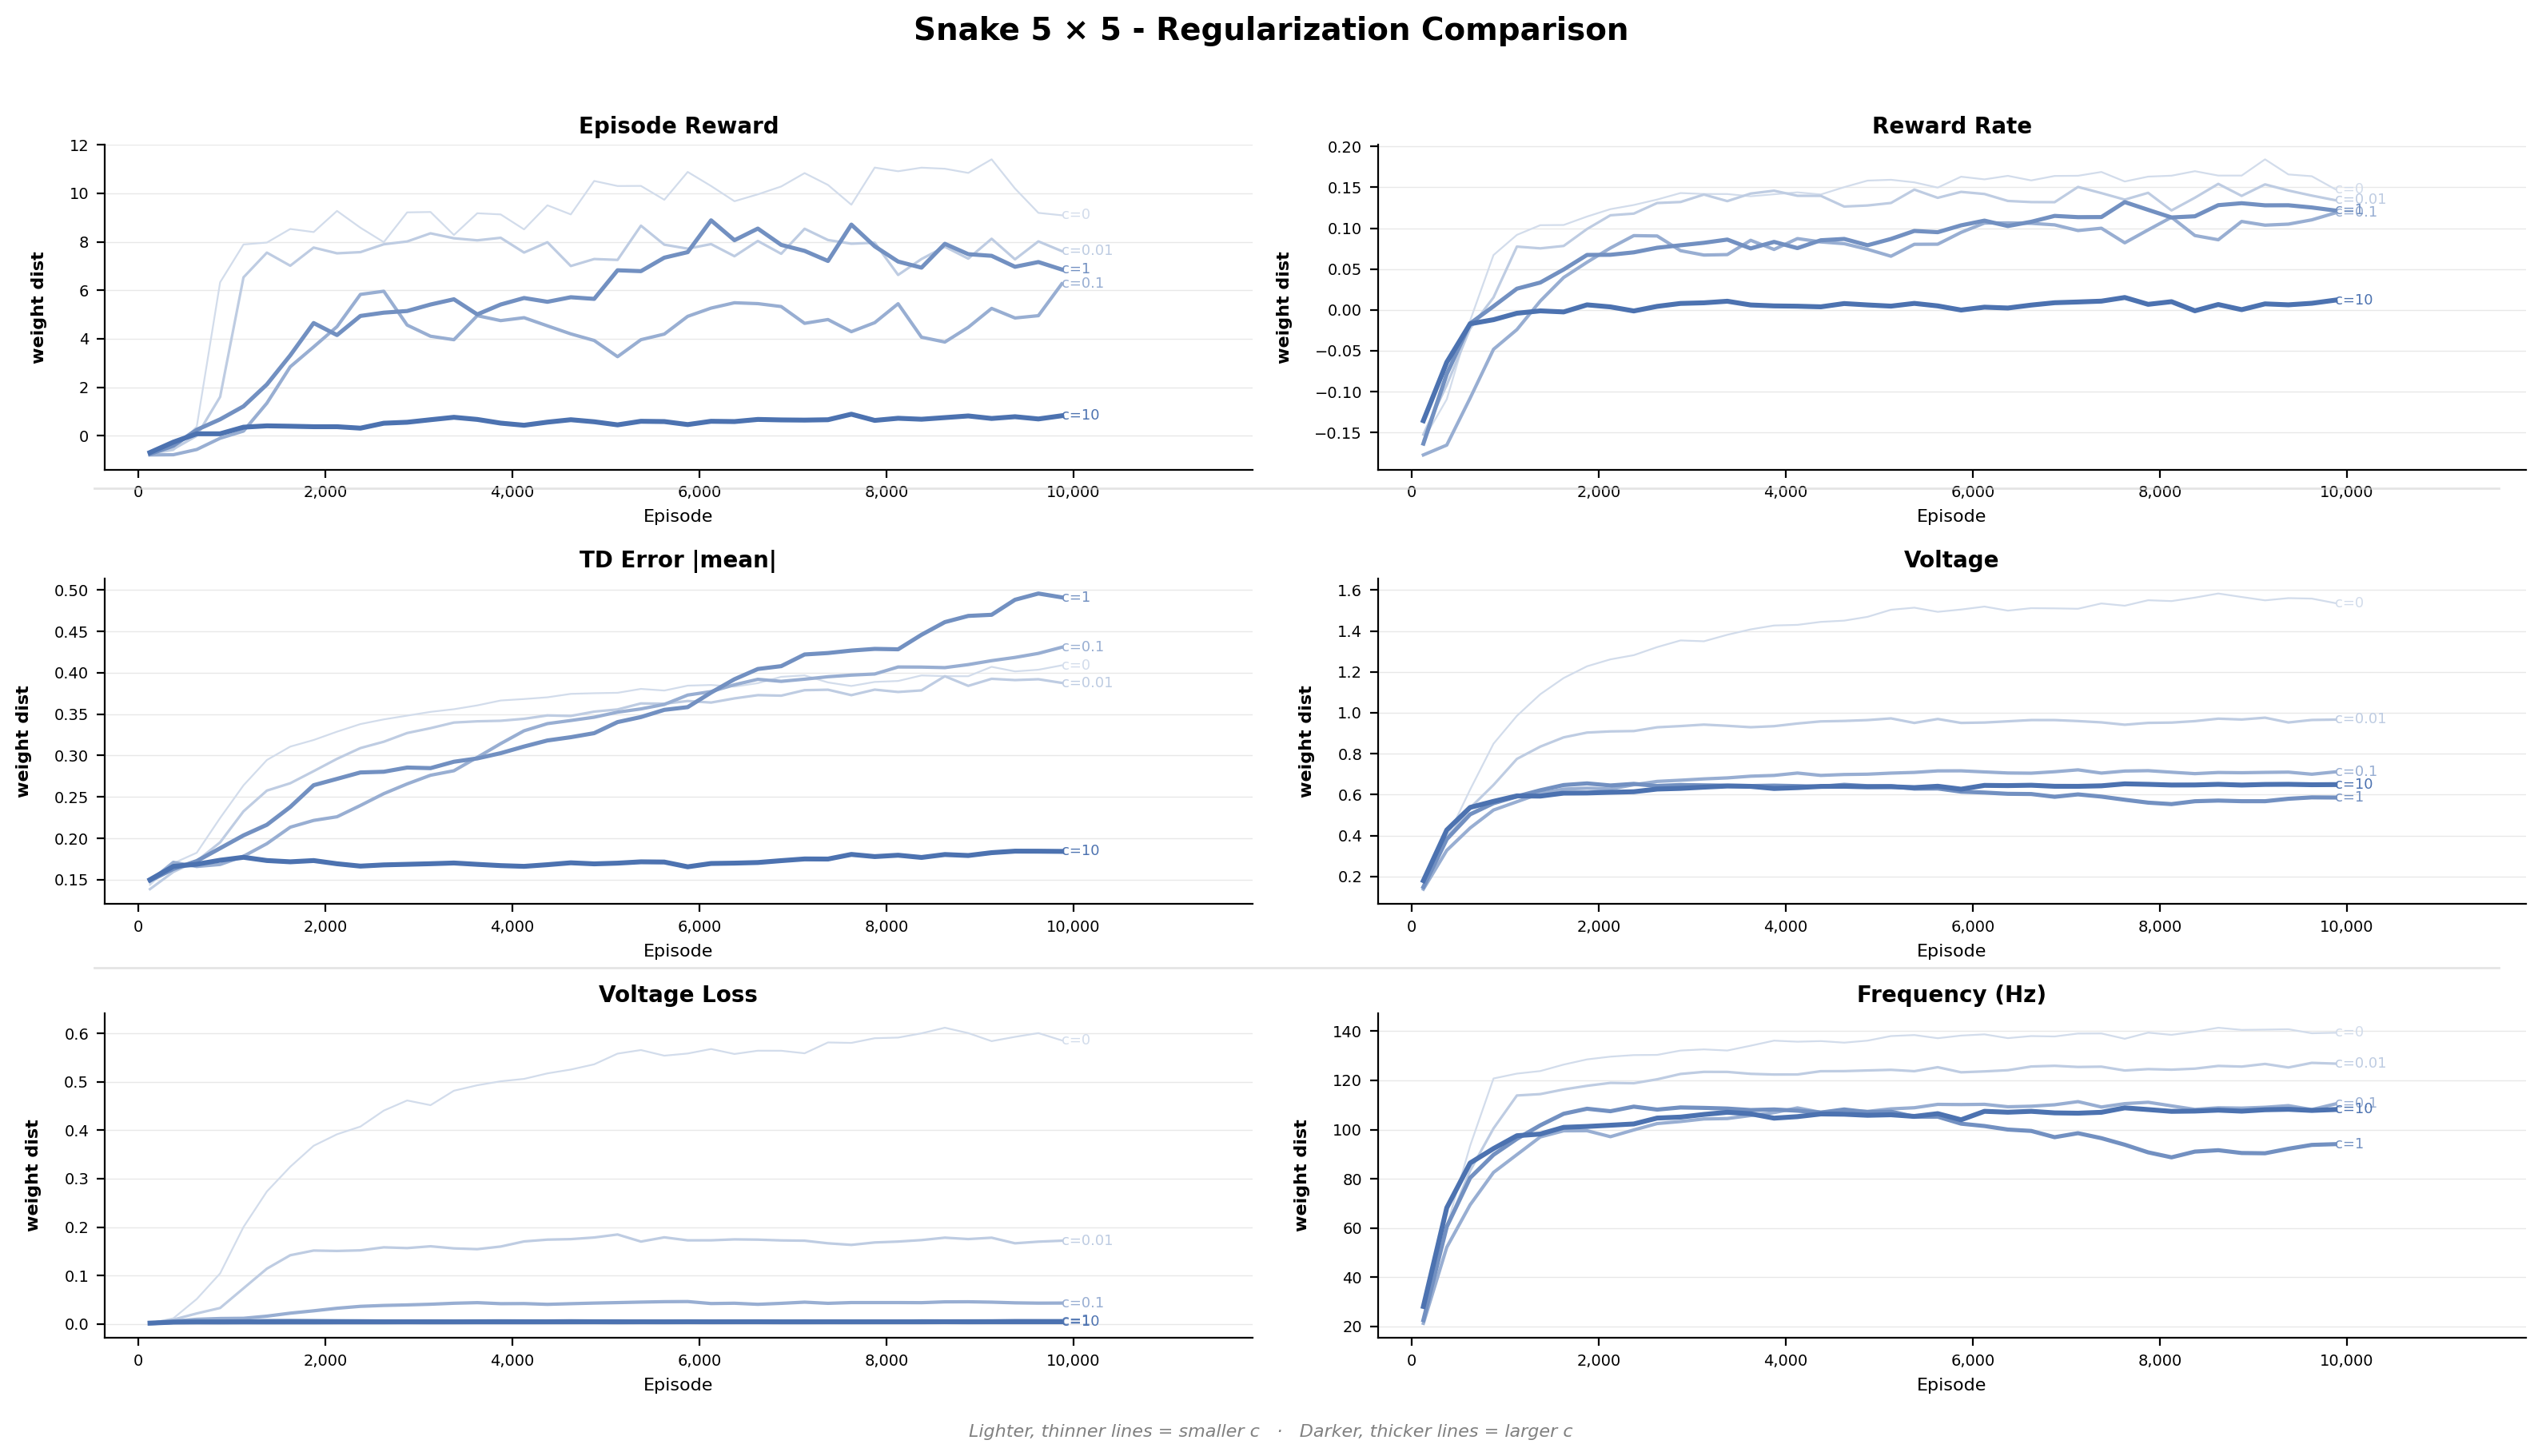
\includegraphics[width=1\linewidth]{images/SnakeRegularizationComparison.png}
    \caption[Reward-based regularization sweep (Snake)]{Reward-based regularization comparison for \emph{weight dist}
    on Snake $5 \times 5$, sweeping over regularization strength $c_{reg}$
    (lighter, thinner lines correspond to smaller values, darker thicker
    lines to larger values). Each panel reports one of the six standard
    metrics over $10,000$ episodes.}
    \label{fig:snake-regularization}
\end{figure}

\section{Best Individual Performances on Snake $5\times5$}

\begin{table}[H]
\caption{Snake results sorted by best mean of 100 Scores (highest to lowest) and Best mean of 100 episode Reward Rates. Each individual run belongs to an experiment, when the name is of the form \emph{variant}($x$) it belongs to the comparative result, otherwise the name discriminates which experiment it belongs to}
\label{tab:snake-best100-score}
\begin{tabular}{l r r r r}
\hline
File & Best100 RewardRate & Best100 Score & Wins & Win \% \\
\hline
symmetric                             & \textbf{0.2113} & \textbf{12.6500} & 14 & 0.1400 \\
weight dist creg 0 (Reg Comp)         & 0.1897 & 12.3100 & \textbf{33} & \textbf{0.3300} \\
weight dist(4)                        & 0.1823 & 11.8200 & 11 & 0.1100 \\
weight dist(3)                        & 0.1776 & 11.7300 & 8  & 0.0800 \\
combined(3)                            & 0.1868 & 11.6000 & 13 & 0.1300 \\
combined lambda 08                     & 0.1761 & 11.5600 & 8  & 0.0800 \\
combined(5)                            & 0.1826 & 11.5100 & 14 & 0.1400 \\
combined(1)                            & 0.1792 & 11.4500 & 6  & 0.0600 \\
adaptive lambda 09                     & 0.1858 & 11.2100 & 3  & 0.0300 \\
adaptive(4)                            & 0.1795 & 11.1300 & 14 & 0.1500 \\
combined(2)                            & 0.1816 & 11.0100 & 11 & 0.1100 \\
weight dist layers 1                   & 0.1755 & 10.9800 & 7  & 0.0700 \\
weight dist(5)                         & 0.1755 & 10.9800 & 7  & 0.0700 \\
adaptive(3)                            & 0.1844 & 10.6500 & 11 & 0.1100 \\
adaptive layers 1                      & 0.1870 & 10.6100 & 5  & 0.0500 \\
weight dist(1)                         & 0.1704 & 10.6100 & 3  & 0.0300 \\
weight dist(2)                         & 0.1743 & 10.5700 & 3  & 0.0300 \\
adaptive lambda 08                     & 0.1816 & 10.5500 & 7  & 0.0700 \\
adaptive lambda 07                     & 0.1808 & 10.4600 & 8  & 0.0800 \\
adaptive(5)                            & 0.1772 & 10.4200 & 7  & 0.0800 \\
adaptive lambda 06                     & 0.1694 & 10.4100 & 6  & 0.0600 \\
combined lambda 07                     & 0.1770 & 10.1900 & 3  & 0.0300 \\
combined(4)                            & 0.1729 & 10.1300 & 6  & 0.0600 \\
weight dist creg 001 (Reg Comp)        & 0.1689 & 9.6000  & 4  & 0.0400 \\
adaptive lambda 04                     & 0.1709 & 9.5800  & 6  & 0.0600 \\
\hline
\end{tabular}
\end{table}

As expected the best metrics belong to the \emph{symmetric} variant, but surprisingly the version of \emph{weight dist} with no regularization beats by a factor of 2.36 in the number of wins and gets very close to the other metrics of the \emph{symmetric} variant.

Here, without taking into account the \emph{symmetric} variant we see that the \emph{combined} rules reliably get to high rewards and win rates, the \emph{adaptive} variant seems to get close to combined, but notably the two top runs do not belong to either \emph{adaptive} nor \emph{combined}, the best two runs, disregarding \emph{symmetric}, are of \emph{weight dist}. This could be because this method has higher variance in the strategies it discovers, and therefore in the rewards it gets, and the other two might converge to more concrete strategies.

\clearpage

\section{Distributed E-prop versus Adaptive E-prop on Pac-Man with
randomized Layouts}
\label{sec:pacman_comparison}

\subsection{Comparison with $\lambda = 0.5$}
Figure~\ref{fig:pacman_comparison} shows a controlled comparison between
distributed e-prop and adaptive e-prop on the Pac-Man randomized layouts
problem, averaged over five independent runs under identical configurations.

\begin{figure}[H]
    \centering
    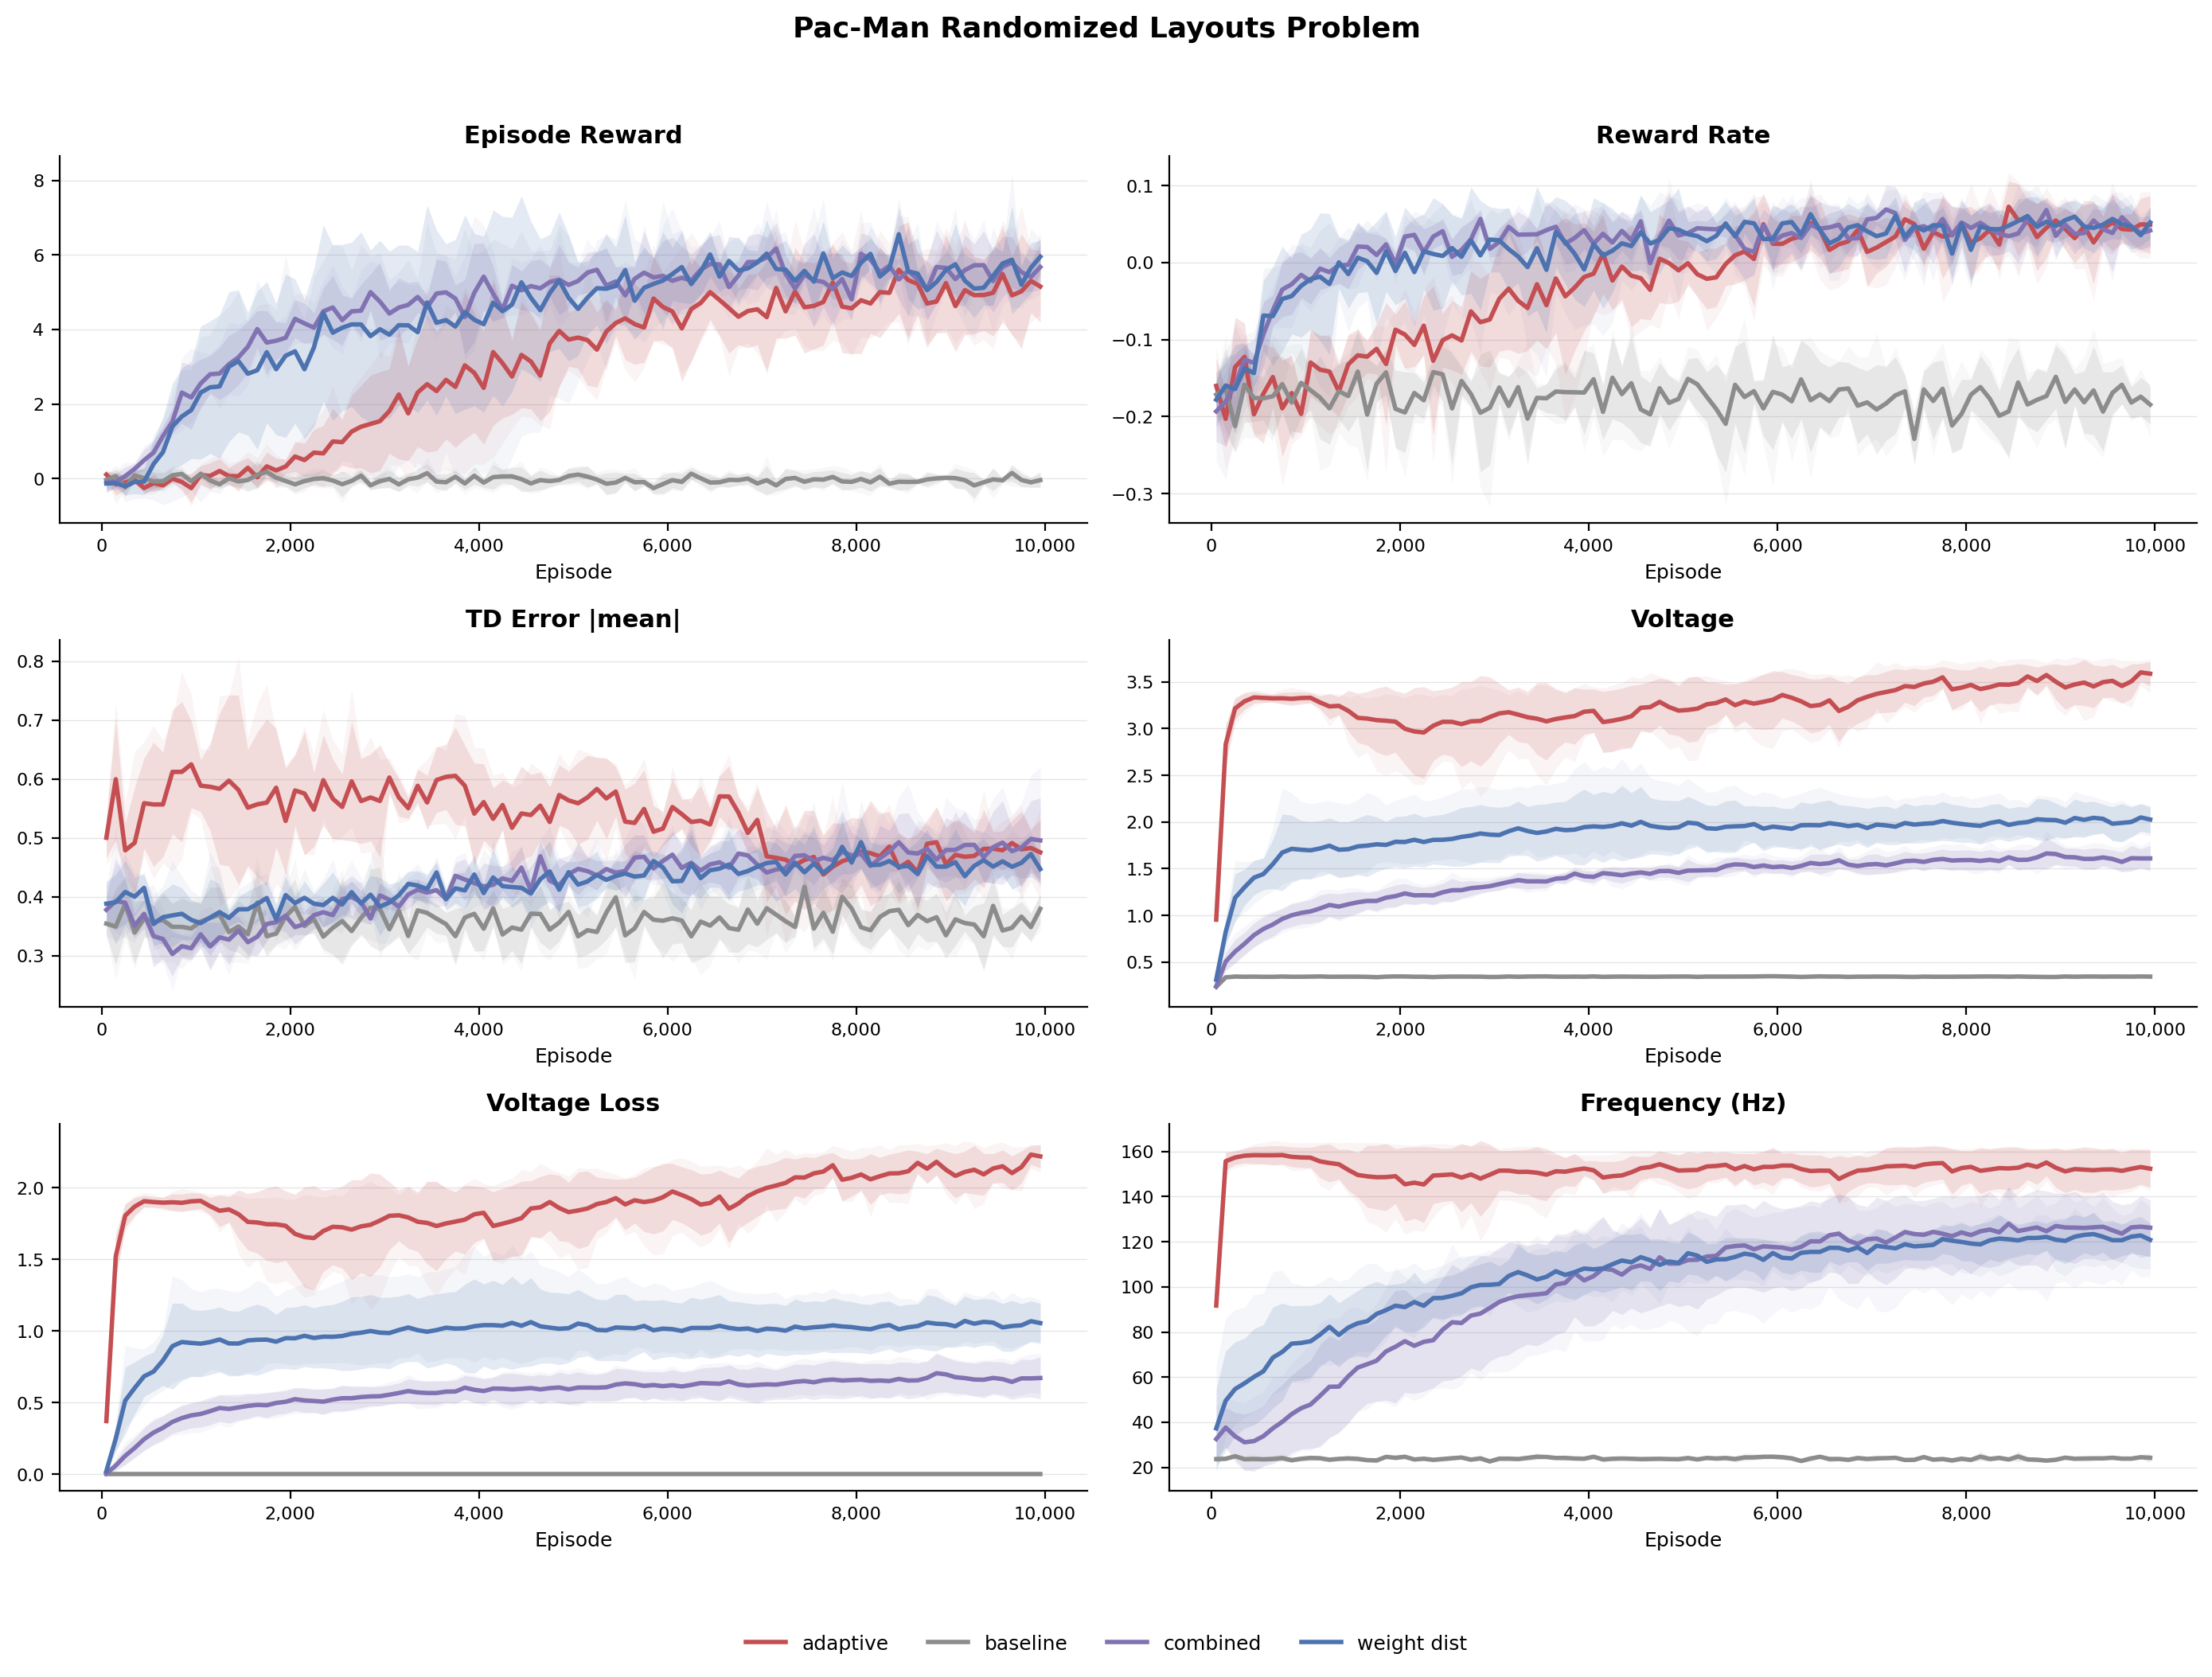
\includegraphics[width=1.0\textwidth]{images/PacManComparison.png}
    \caption[Distributed vs.\ adaptive e-prop (Pac-Man)]{Controlled comparison of distributed e-prop variants and
    adaptive e-prop on the Pac-Man randomized layouts problem, averaged
    over five independent runs with shaded standard deviation bands.
    Top row: episode reward and reward rate. Middle row: absolute TD
    error and mean membrane voltage. Bottom row: voltage loss and mean
    firing frequency.}
    \label{fig:pacman_comparison}
\end{figure}

Under equal conditions, distributed e-prop variants reach higher episode
rewards than adaptive e-prop, though both converge to comparable reward
rates by the end of training. The TD error is more unstable for adaptive
e-prop, and its voltage and frequency metrics are both worse and more
variable throughout training, consistent with the pattern observed in the
Snake experiments. The \emph{combined} variant again behaves more
similarly to the distributed e-prop family than to adaptive e-prop across
all metrics, reinforcing the observation from
Section~\ref{sec:snake_comparison} that its update is dominated by the
perturbation-based signal in this implementation.

A further limitation of these results is the length of the experiments.
Both algorithms show signs of continued improvement at the end of the
10,000 episode training horizon, particularly in the reward rate plots,
suggesting that the performance gap between them could narrow or widen
further with longer training. The conclusions drawn here should therefore
be understood as reflecting behavior within this specific training budget.

Taken together, these results reinforce the picture that emerged from the
Snake experiments: distributed e-prop and adaptive e-prop make different
assumptions about the network dynamics, exploit different sources of credit
assignment information, and appear to thrive under different operating
conditions. Understanding when and why one outperforms the other remains
an important open question that a more systematic study varying neuron
configuration, network size, task structure, and training length would be
needed to resolve.

The baseline, as in snake stays flat on all metrics, not learning at all.

Figure~\ref{fig:value_function_comparison} provides a qualitative view of
the value function learned by each algorithm at three different stages of
training, from earlier episodes at the top to later episodes at the bottom.

\begin{figure}[H]
    \centering
    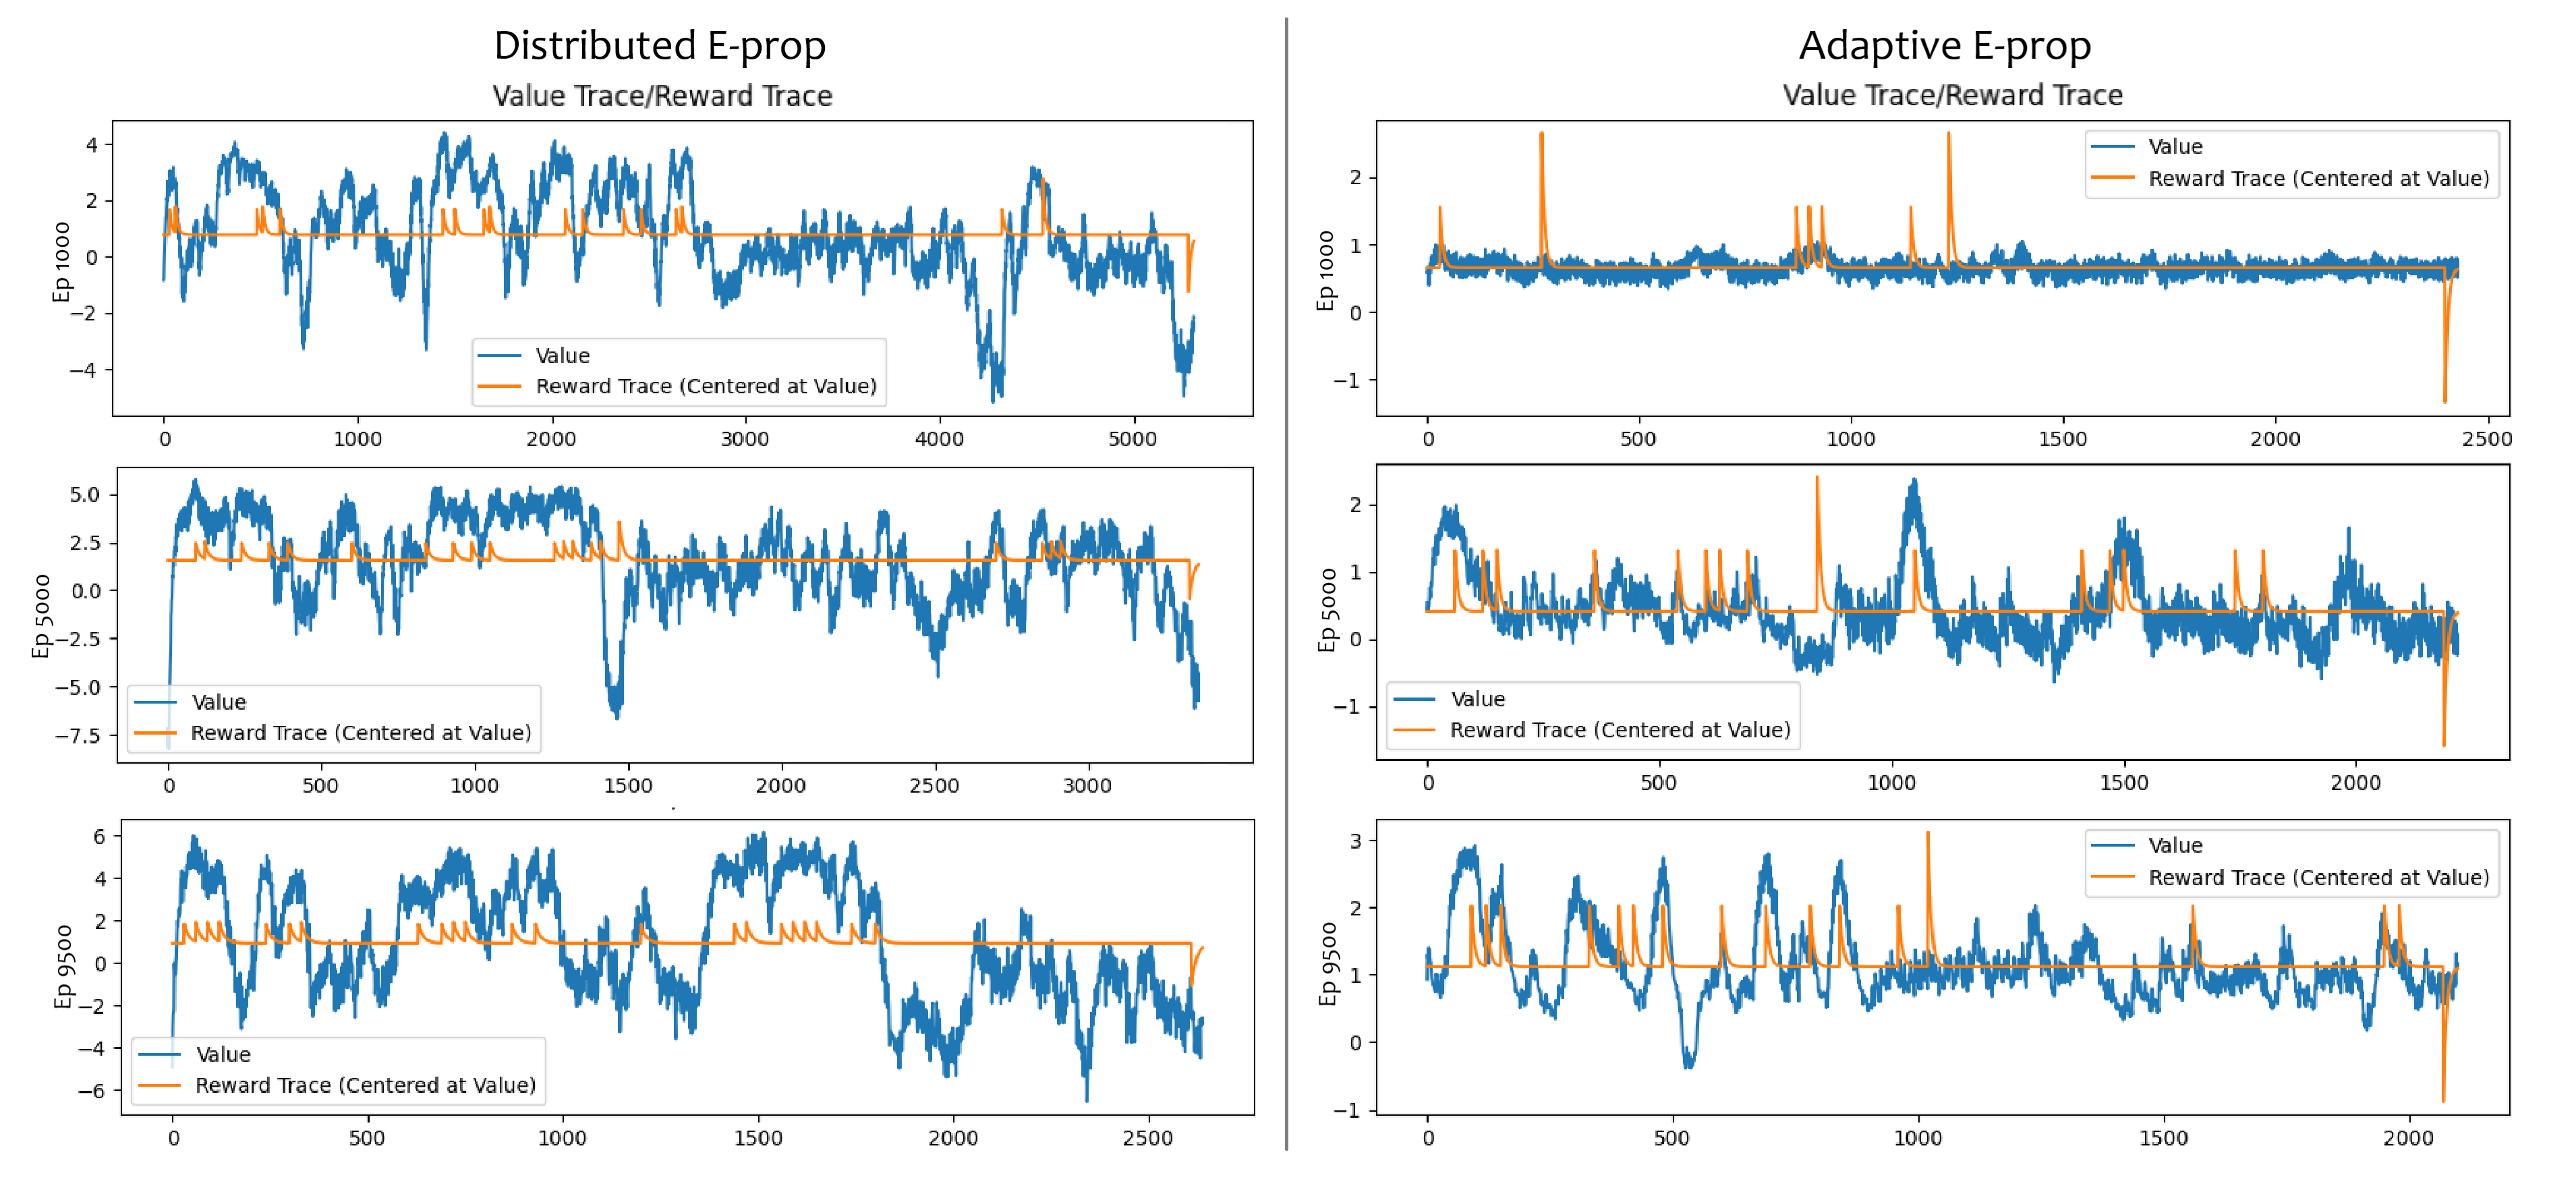
\includegraphics[width=1.0\textwidth]{images/ValueFunctionPacManComparison.png}
    \caption[Value traces: distributed vs.\ adaptive e-prop (Pac-Man)]{%
    Value function and centered reward trace for distributed e-prop (left) and
    adaptive e-prop (right) on Pac-Man, at three stages of a single training run,
    ordered from earlier (top) to later (bottom). As in the Snake value-trace
    figure, the two axes measure different things: down a column the rows are
    separate training snapshots, not one continuous signal, while across a panel the
    horizontal axis is the frame number within a single game at that stage, and
    restarts from zero, so panels spanning games of different lengths differ in
    width. The blue trace is the learned value estimate $V_t$; the orange trace is
    the reward trace, shifted to sit at the value level so
    that reward events can be read directly against the value. Vertical scales are
    independent per panel, since the magnitude of the learned value grows over
    training.}
    \label{fig:value_function_comparison}
\end{figure}

Across all three stages of training, the value function learned by
distributed e-prop tracks the reward trace more closely and with greater
dynamic range than that of adaptive e-prop, which remains comparatively
flat and close to a constant baseline throughout training. This mirrors
what was observed in the Snake experiments, and is again at odds with the
TD error plots: the absolute TD error grows over the course of training
for distributed e-prop while decreasing for adaptive e-prop. As discussed
in Section~\ref{sec:snake_comparison}, a flat value function naturally
produces small TD errors without necessarily carrying useful information,
while a more expressive and dynamic estimate will make larger predictions
that can be more wrong on any given step. The TD error should therefore
not be read as a measure of critic quality in isolation, and this
observation is particularly clear here.

An example of the richer value representation learned
by distributed e-prop can be seen in the traces, where on several occasions
the value estimate drops sharply into negative territory immediately before
a large positive reward spike of magnitude 2, corresponding to the agent
eating a frightened ghost. This indicates that the agent expected to die
in that moment, likely because it was in close proximity to the ghost, but
instead managed to eat it. The critic has evidently learned to associate
ghost proximity with danger, which is a meaningful and correct association in most
circumstances, but one that fails to account for the capsule state that
makes the ghost vulnerable. This kind of structured but imperfect prediction
is only possible if the value function has learned something genuine about
the task dynamics, and it stands in clear contrast to the flat adaptive
e-prop estimates which neither anticipate danger nor respond to the
ghost-eating reward in any structured way.

\subsection{No Integration During Refractory Period}
\label{subsec:no_refractory_integration}

\begin{figure}[htpb]
    \centering
    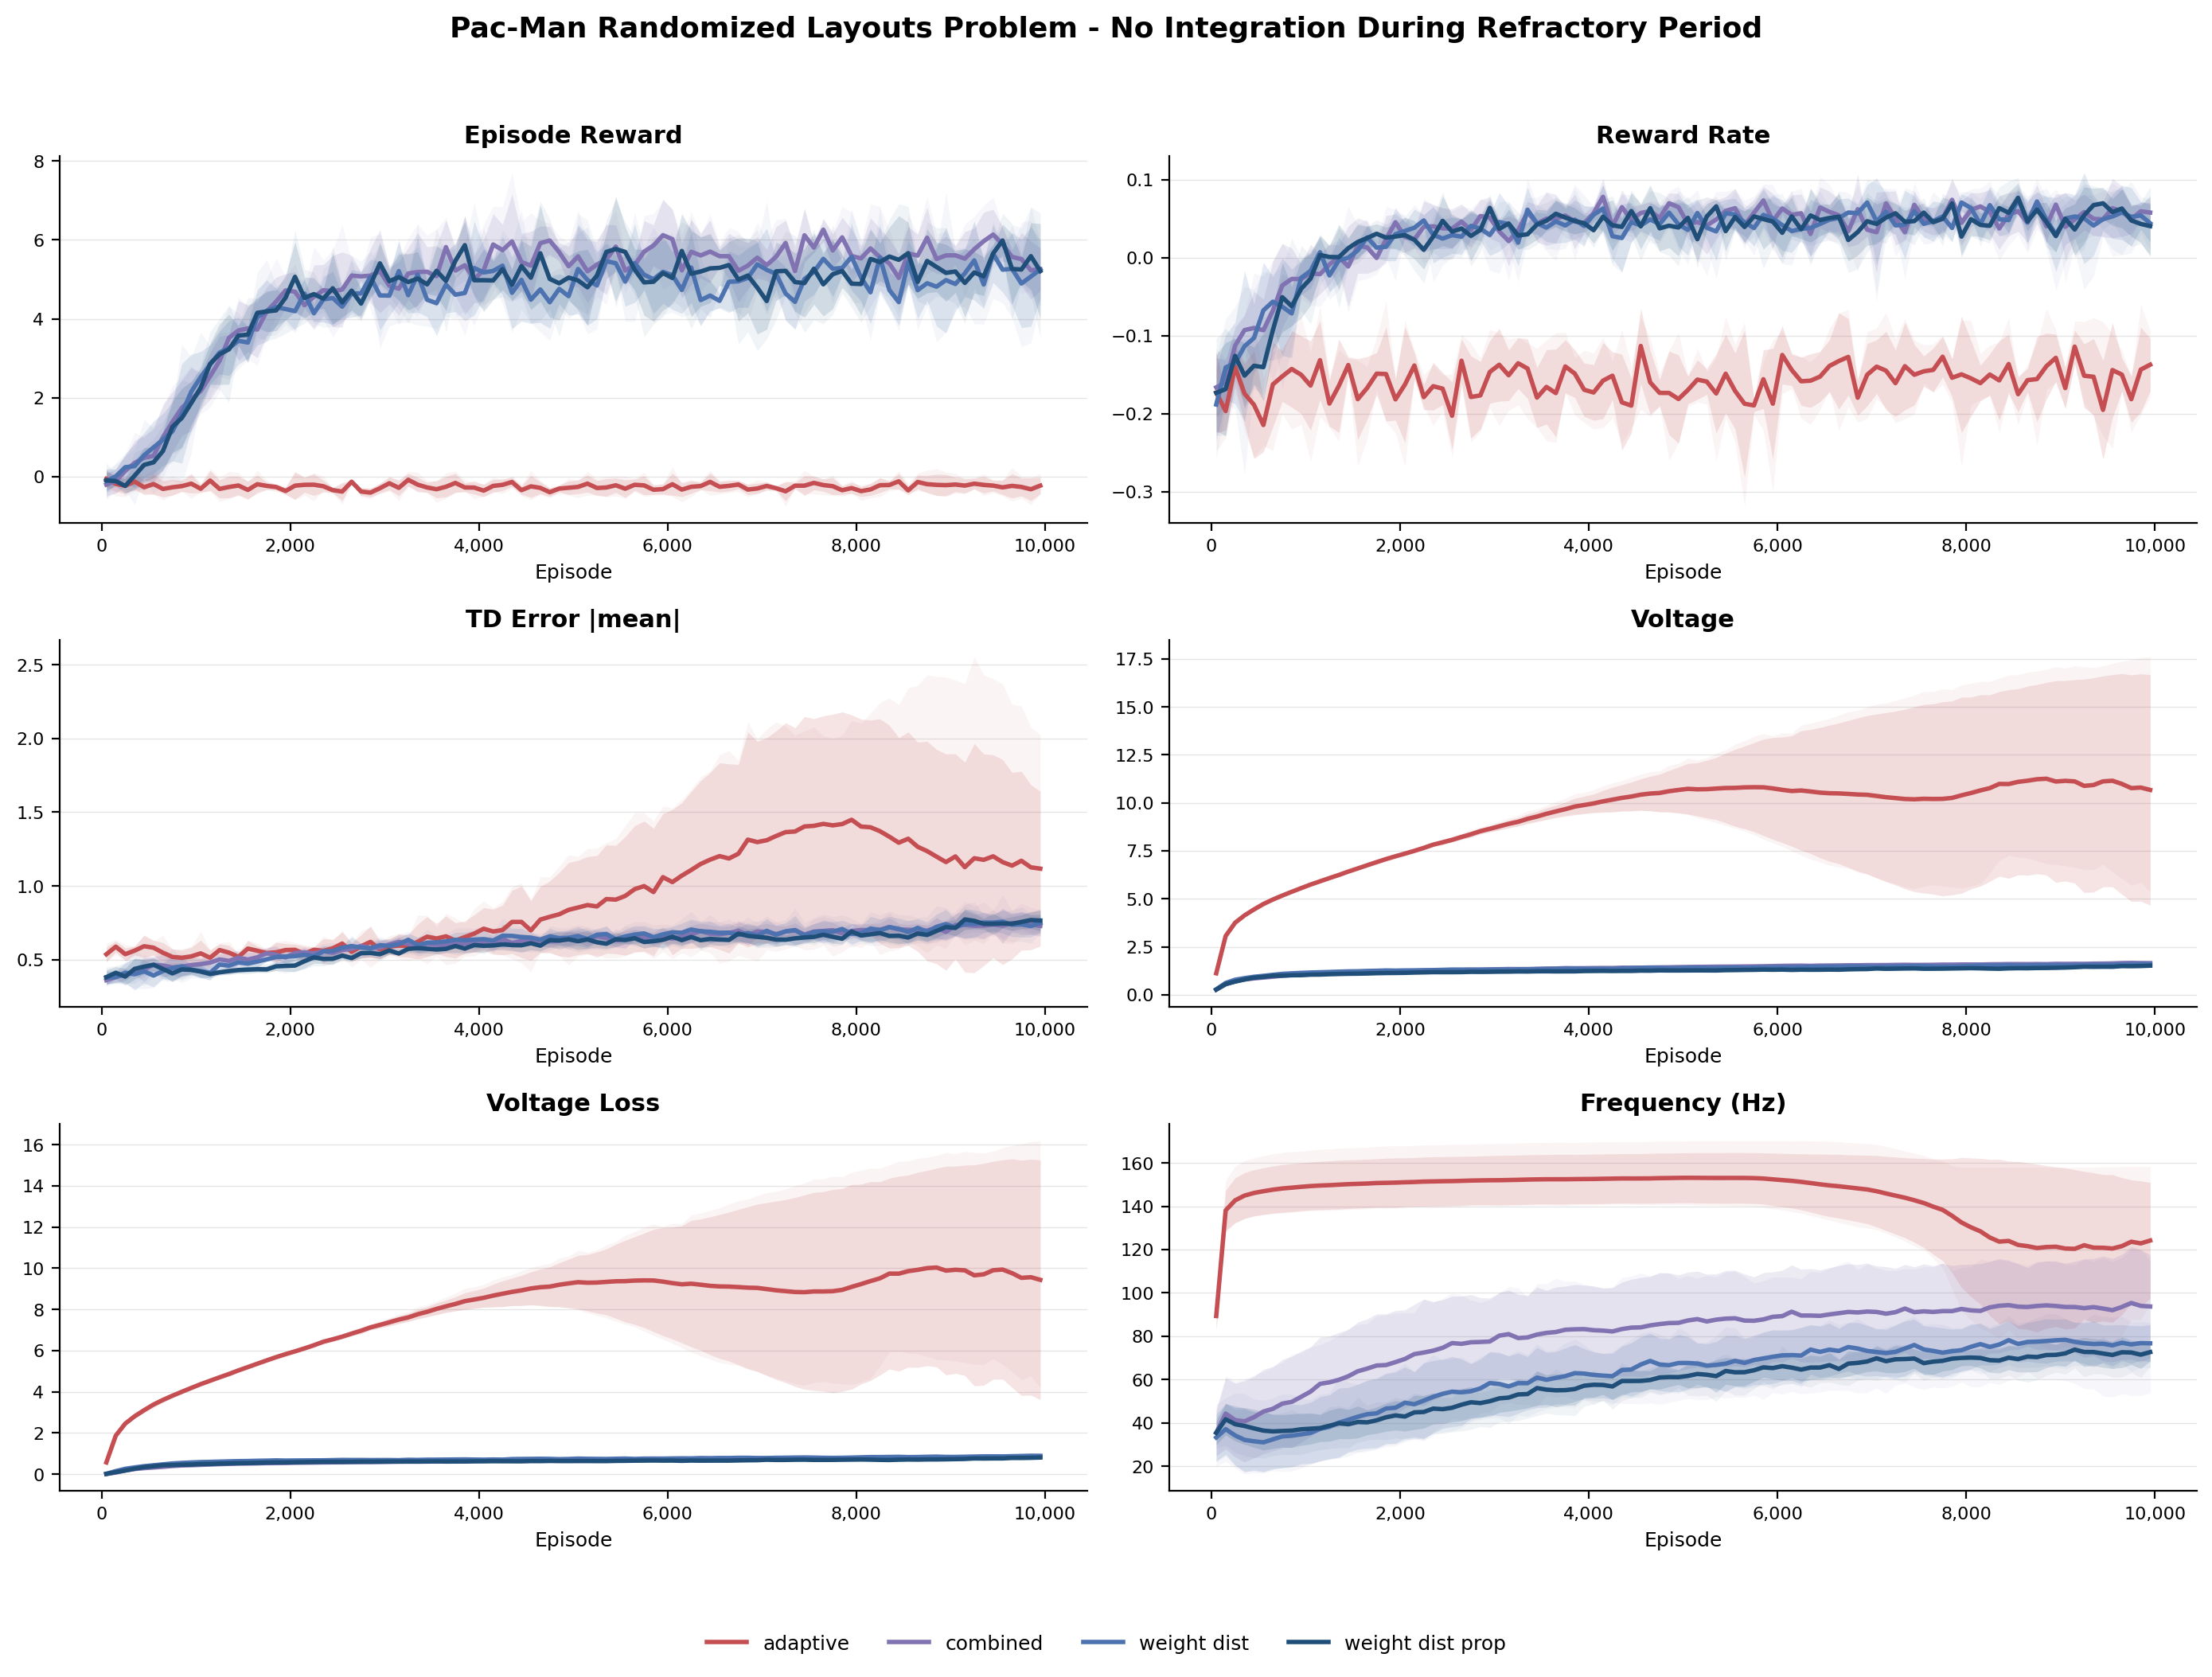
\includegraphics[width=1.0\textwidth]{images/PacManComparisonNoIntegration.png}
    \caption[No-refractory-integration comparison (Pac-Man)]{Comparison of distributed e-prop variants and adaptive e-prop
    on the Pac-Man randomized layouts problem under the
    no-integration-during-refractory-period neuron variant, with reward
    trace decay set to 0.1 for all variants, averaged over five independent
    runs with shaded standard deviation bands. Top row: episode reward and
    reward rate. Middle row: absolute TD error and mean membrane voltage.
    Bottom row: voltage loss and mean firing frequency.}
    \label{fig:pacman_no_integration}
\end{figure}

This experiment runs both algorithms under the neuron variant that does not integrate inputs during the refractory period, with the reward trace decay set to 0.1 for all variants. Standard
e-prop handles this variant poorly, its eligibility trace derivation assumes
integration continues during the refractory period, and violating this
assumption introduces inconsistencies between the forward dynamics and the
learning rule. Distributed e-prop is less sensitive to this assumption since
its credit assignment is based on perturbation correlations rather than on
a precise analytical decomposition of the gradient.

The results reflect this difference clearly. Adaptive e-prop barely learns
under this configuration, with episode reward remaining near zero and
voltage and frequency metrics diverging severely throughout training. The
distributed e-prop variants, by contrast, learn the task successfully and
maintain well-regulated spiking dynamics. Among them, \emph{combined}
achieves marginally higher episode rewards but at the cost of worse
frequency metrics, while \emph{weight dist prop} finds less active
configurations than both \emph{combined} and \emph{weight dist} while
maintaining comparable task performance. This contrasts with the Snake
results in Section~\ref{sec:snake_comparison}, where structured routing
was clearly detrimental to \emph{weight dist}; here it appears to find
sparser activity patterns that are sufficient for the task, though we do
not offer a mechanistic explanation for this difference.

The advantage of distributed e-prop in this setting is not merely a
consequence of a more favorable hyperparameter configuration; it reflects
a genuine difference in how the two rules interact with the network
dynamics when the refractory period assumption is violated. Whether this
robustness extends to other neuron variants or network configurations
remains an open question.

\subsection{Lambda Comparison}
\label{subsec:pacman_lambda_comparison}

Figure~\ref{fig:pacman_lambda} repeats the decay-factor sweep introduced in
Section~\ref{sec:snake_lambda_comparison} on the Pac-Man randomized layouts
problem, this time comparing adaptive e-prop and the structured-routing
distributed variant \emph{weight dist prop}. As anticipated there, the
two tasks produce markedly different pictures of which learning rule
tolerates a wide range of $\lambda$, and it is this contrast, that is most informative.

The distributed variant used throughout this comparison is run under the
\emph{no-integration-during-refractory-period} neuron variant introduced in
Section~\ref{subsec:no_refractory_integration}. This choice is
deliberate: among the configurations evaluated on the Pac-Man randomized
layouts problem, this variant was one of the strongest performers for 
the distributed eprop variants, and it also produced the most favorable
voltage and frequency statistics of the configurations tested, remaining
well-regulated where the standard-refractory configuration showed more
pronounced drift. Using this variant for the $\lambda$ sweep therefore
gives distributed e-prop a comparatively stable starting point from which
to isolate the effect of $\lambda$ specifically. Adaptive
e-prop, by contrast, is shown here under its standard configuration, since
Section~\ref{subsec:no_refractory_integration} found this same neuron variant
to be markedly detrimental to adaptive e-prop; the
two algorithms are therefore each shown under the neuron configuration
most favorable to them individually, which should be kept in mind when
comparing the absolute stability of their voltage and frequency curves
below.

\label{sec:lambda_comparison}
\begin{figure}[htbp]
    \centering
    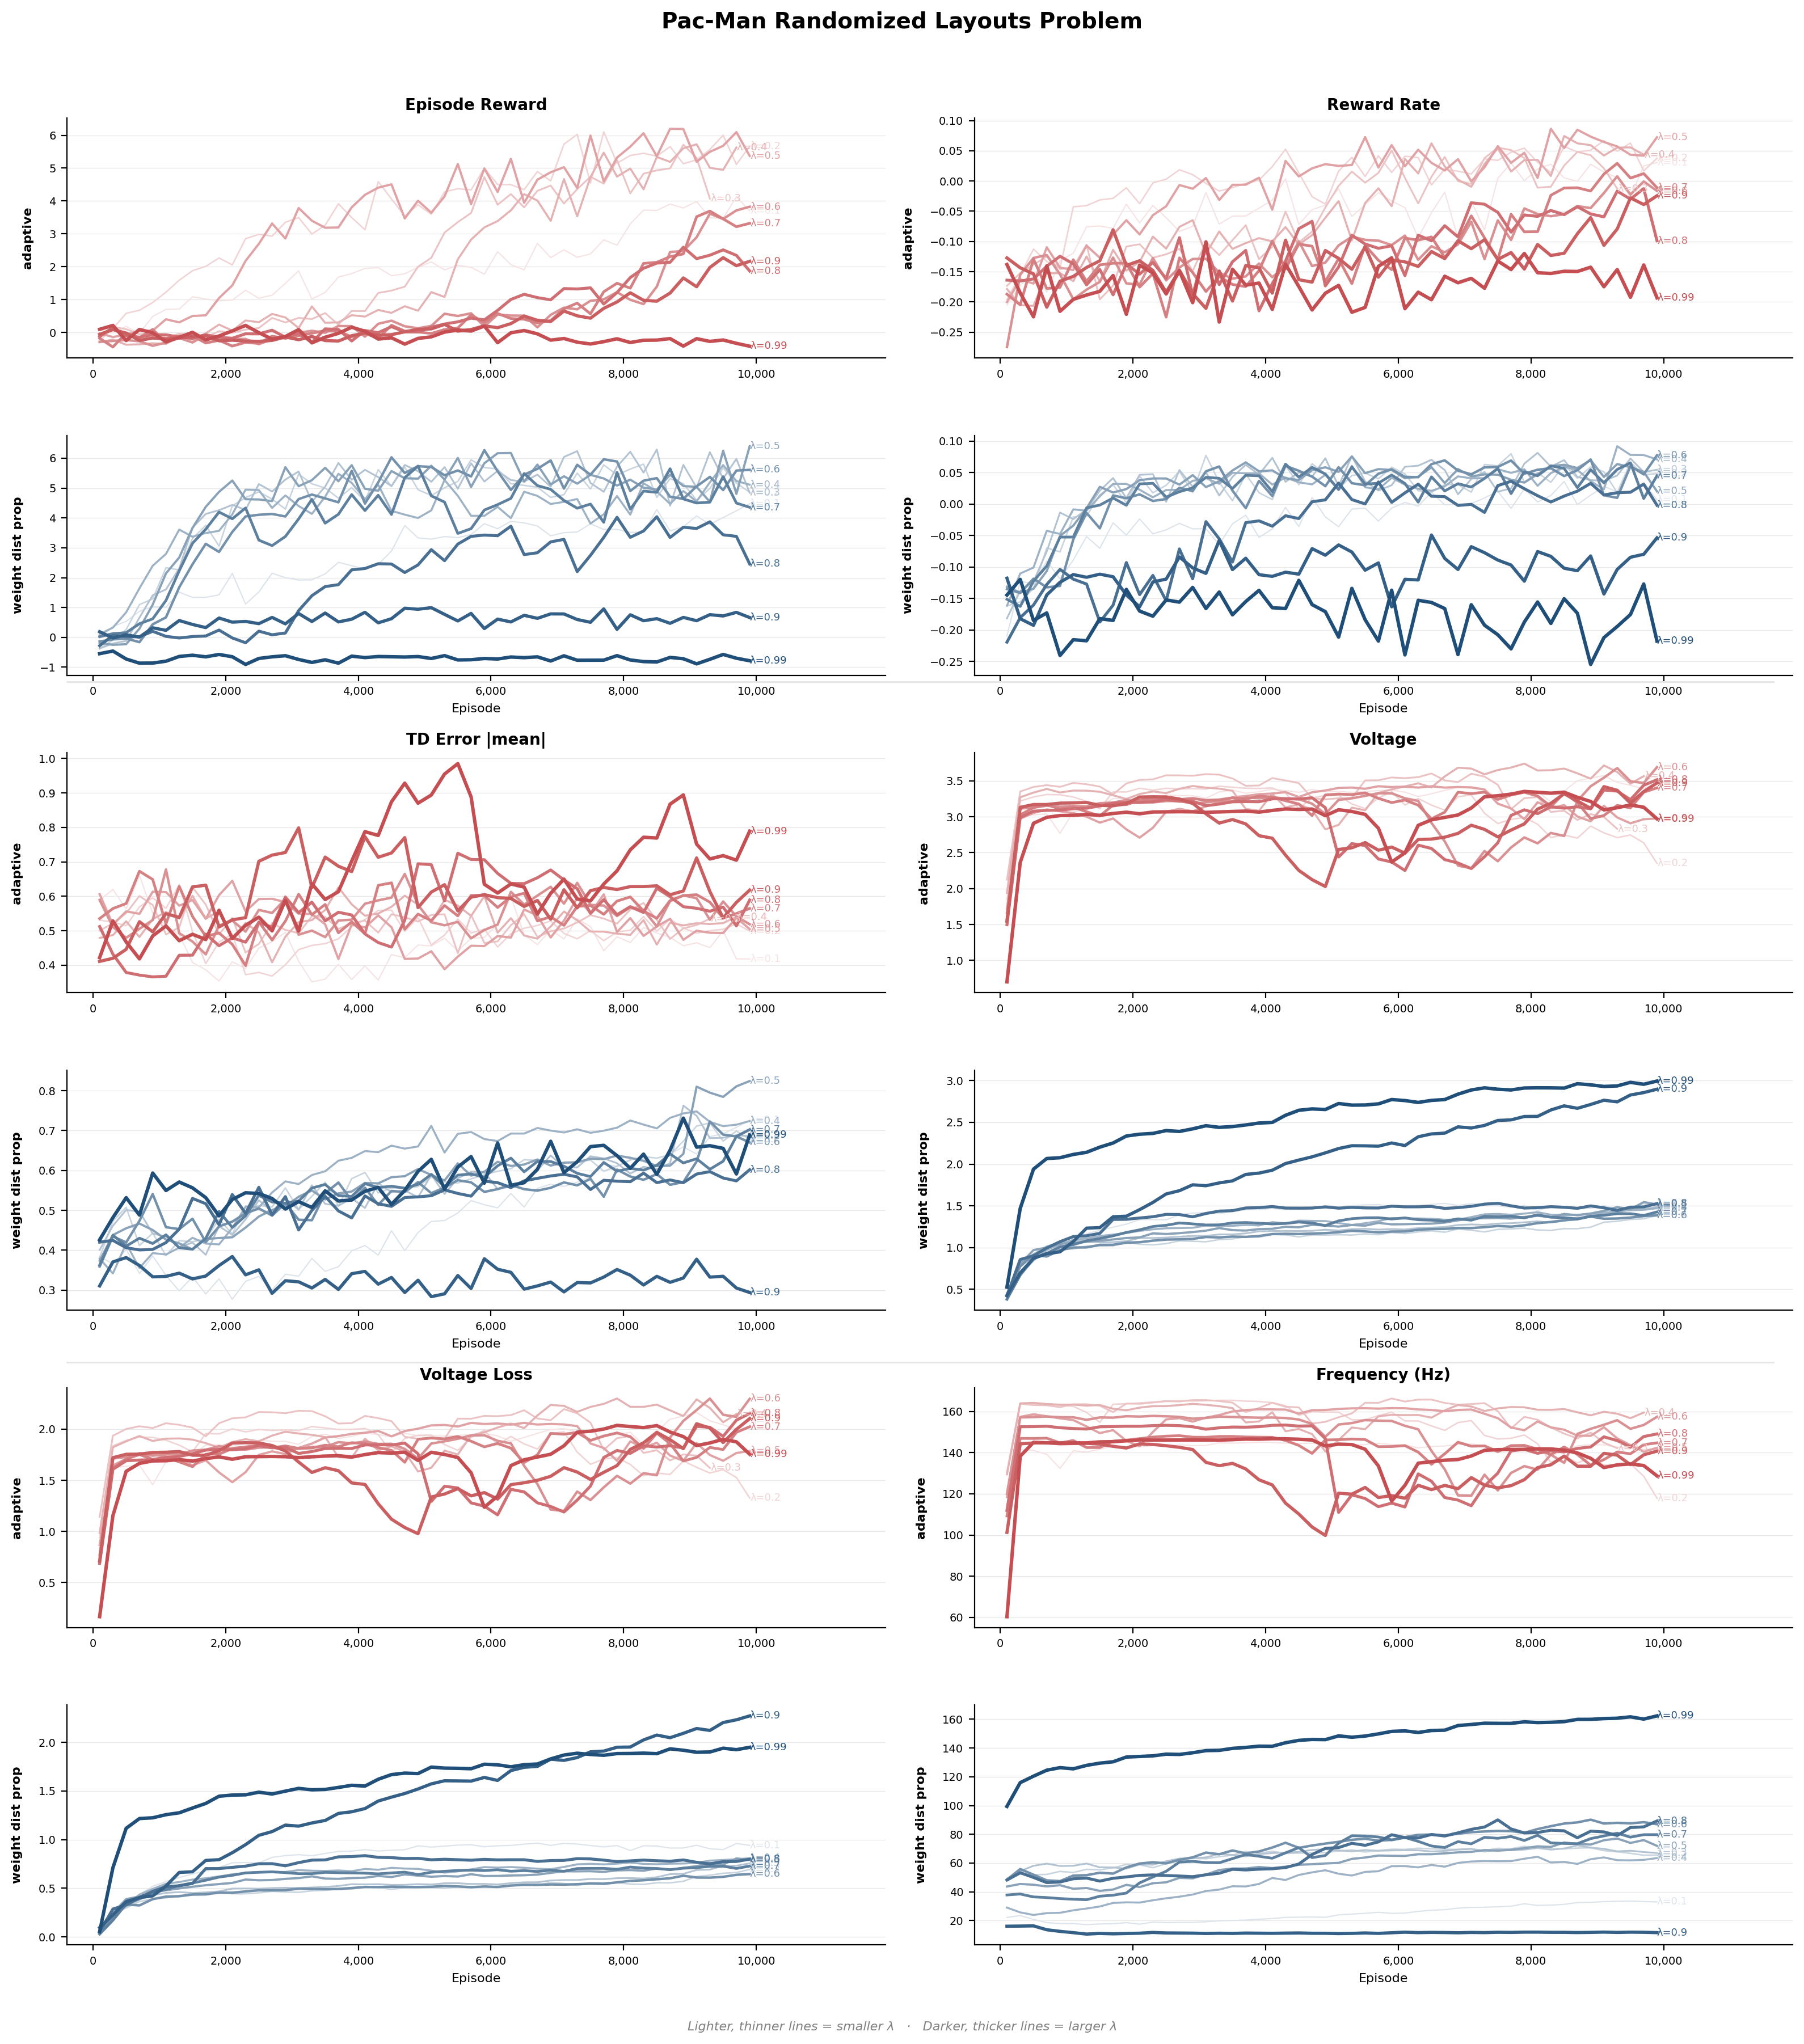
\includegraphics[width=\textwidth]{images/PacManComparisonLambdaGroups.png}
    \caption[Lambda sweep on Pac-Man]{Training performance across $10,000$
    episodes on the Pac-Man randomized layouts problem for adaptive e-prop
    (red) and \emph{weight dist prop} (blue), across varying decay
    factors $\lambda \in \{0.1, 0.2, \ldots, 0.9, 0.99\}$ (lighter, thinner
    lines correspond to smaller $\lambda$; darker, thicker lines to larger
    $\lambda$). Metrics reported include episode reward, reward rate, TD
    error (mean), voltage, voltage loss, and frequency (Hz).}
    \label{fig:pacman_lambda}
\end{figure}
For both algorithms, the best episode reward and reward rate are reached
around $\lambda = 0.5$, with performance generally falling off as
$\lambda$ increases. As
discussed in Section~\ref{sec:snake_lambda_comparison}, a larger $\lambda$
trades a longer credit-assignment reach for a higher-variance trace, and
on this task a short horizon already appears sufficient to capture the
relevant action-reward delays, so little is gained, and much is lost, by
extending it further. The more informative difference between the two
rules lies not in where the optimum falls but in the \emph{shape} of
learning across the sweep, and in this respect the picture is the reverse
of what was seen on Snake. Adaptive e-prop shows a markedly inconsistent
onset of learning across $\lambda$ values: several of its curves remain
flat for an extended initial period before rising, echoing the slow,
feedback-alignment-dependent start already observed in
Section~\ref{subsec:snake-depth-comparison}, with no clear relationship between
$\lambda$ and how long this initial delay lasts. The distributed variant,
by contrast, begins improving promptly across most of the sweep, with
$\lambda \in \{0.4, 0.5, 0.6\}$ all reaching comparable, strong performance
early in training. The clear losers for distributed e-prop in this run are
the larger values $\lambda \in \{0.8, 0.9, 0.99\}$, which trail the rest of
the sweep throughout training.

Interestingly, these three under-performing runs do not all fail in the
same way. The voltage and frequency panels show that the $\lambda = 0.8$
and $\lambda = 0.99$ runs drift toward the same runaway, pathologically
high-voltage and high-frequency regime, climbing steadily across training
instead of converging. The $\lambda = 0.9$ run, however, moves in the
opposite direction, with voltage and firing frequency trending lower. 
Both extremes are consistent with the 
loss of useful credit-trace information at a poorly
chosen $\lambda$, but they point to two distinct failure modes available
to this learning rule: one in which the network drifts toward saturated,
uninformative firing, and another in which it drifts toward excessive
silence and equally uninformative activity. Because this comparison
reflects a single run per $\lambda$ value, in the same sense already
flagged for the $\lambda = 0.4$ failure of \emph{combined} on Snake in
Section~\ref{sec:snake_lambda_comparison}, we cannot determine from this
experiment alone whether $\lambda = 0.9$ reliably falls toward the
low-activity failure mode or whether this particular run simply landed on
one side of what might be a more variable outcome across seeds; it is
equally possible that a different run at $\lambda = 0.9$ would drift
toward the high-activity pathology instead, or even stabilize.
What the figure does establish is that both failure modes are reachable by
the same learning rule under similar conditions, which is itself useful to
know even without a settled account of what determines which one a given
run falls into.

Taken together with the Snake comparison in
Section~\ref{sec:snake_lambda_comparison}, these results reinforce the
view that neither learning rule is uniformly more robust to the choice of
$\lambda$. On Pac-Man, distributed e-prop tolerates a wider range of
$\lambda$ before its dynamics degrade, and begins learning consistently
once a suitable range is found, whereas adaptive e-prop's reliance on an
approximate feedback pathway appears to make its time-to-learn less
predictable across $\lambda$, independently of where its eventual
performance ceiling lies, the opposite of the ordering found on Snake. At
the same time, the divergent failure modes observed for distributed e-prop
at large $\lambda$ here indicate that its apparent robustness should not
be overstated: poor choices of $\lambda$ can still destabilise the
network, simply through more than one route, and confirming how
consistently each route is associated with a given $\lambda$ would require
repeated runs beyond the single-seed comparisons presented in this
chapter.

\section{Best Individual Performances on Pac-Man Randomized Layouts}

\begin{table}[H]
\caption{Pac-Man results sorted by best mean of 100 Scores (highest to lowest) and Best mean of 100 episode Reward Rates. Each individual run belongs to an experiment, when the name is of the form \emph{variant}($x$) it belongs to the comparative result, otherwise the name discriminates which experiment it belongs to.}
\label{tab:pacman-best100-score}
\begin{tabular}{l r r r r}
\hline
File & Best100 RewardRate & Best100 Score & Wins & Win \% \\
\hline
weight dist(1)                    & 0.1039 & \textbf{8.2030} & 10 & 0.1000 \\
weight dist(3)                    & 0.1106 & 8.1440 & 9  & 0.0900 \\
weight dist(4)                    & \textbf{0.1400} & 7.9890 & 8  & 0.0800 \\
combined (NIDRP)(3)               & 0.1075 & 7.9420 & 10 & 0.1000 \\
weight dist(2)                    & 0.1050 & 7.8270 & 4  & 0.0400 \\
adaptive(2)                       & 0.1214 & 7.8090 & 6  & 0.0600 \\
adaptive(1)                       & 0.1195 & 7.7530 & \textbf{14} & \textbf{0.1400} \\
weight dist prop lambda 03        & 0.1173 & 7.6490 & 8  & 0.0800 \\
combined(1)                       & 0.1090 & 7.6140 & 7  & 0.0700 \\
adaptive lambda 05                & 0.1228 & 7.6030 & 3  & 0.0300 \\
combined (NIDRP)(2)               & 0.1046 & 7.4820 & 5  & 0.0500 \\
combined (NIDRP)(5)               & 0.1081 & 7.4760 & 10 & 0.1000 \\
combined(3)                       & 0.1127 & 7.4470 & 4  & 0.0400 \\
combined (NIDRP)(1)               & 0.1089 & 7.4360 & 3  & 0.0300 \\
combined(4)                       & 0.1085 & 7.3770 & 4  & 0.0400 \\
weight dist prop (NIDRP)(2)       & 0.1064 & 7.3720 & 11 & 0.1100 \\
weight dist (NIDRP)(1)            & 0.1074 & 7.3230 & 3  & 0.0300 \\
weight dist prop (NIDRP)(3)       & 0.1085 & 7.2990 & 5  & 0.0500 \\
weight dist (NIDRP)(3)            & 0.1052 & 7.1880 & 2  & 0.0200 \\
weight dist prop lambda 02        & 0.1122 & 7.1290 & 6  & 0.0600 \\
weight dist (NIDRP)(4)            & 0.1075 & 7.0670 & 3  & 0.0300 \\
weight dist (NIDRP)(2)            & 0.1081 & 6.4350 & 2  & 0.0200 \\
weight dist prop lambda 04        & 0.1204 & 6.3090 & 1  & 0.0100 \\
adaptive lambda 03                & 0.1069 & 6.3040 & 1  & 0.0100 \\
adaptive lambda 01                & 0.1654 & 4.8430 & 0  & 0.0000 \\
\hline
\end{tabular}
\vspace{2mm}
\footnotesize{NIDRP = No Integration During Refractory Period.}
\end{table}

The performance metrics in this environment are clearly dominated by the variants of distributed e-prop, but adaptive did have the run with more wins. With regards to the $Best100$ metrics the two best runs belong to \emph{weight dist}. Only 5 adaptive runs are in this top-26 table, which align with the charts, that show the distributed variants learning faster and converging to a higher ceiling, although, as noted in before, adaptive e-prop seems to need more time to learn in some settings, and it can overtake distributed e-prop if given enough time.

\clearpage
\section{Connect Four with Sparse Reward}
\label{sec:connect_four}

Connect Four is the most demanding of the environments considered here: the reward is sparse,
arriving only at the end of a game, so the agent must propagate credit across an entire game from a
single terminal outcome. Figure~\ref{fig:connect-four} reports the six standard metrics for the four
learning rules (adaptive e-prop, \emph{weight dist}, \emph{combined}, and the \emph{baseline}) on
this task, with one run per configuration over roughly $400{,}000$ episodes.

\begin{figure}[htpb]
    \centering
    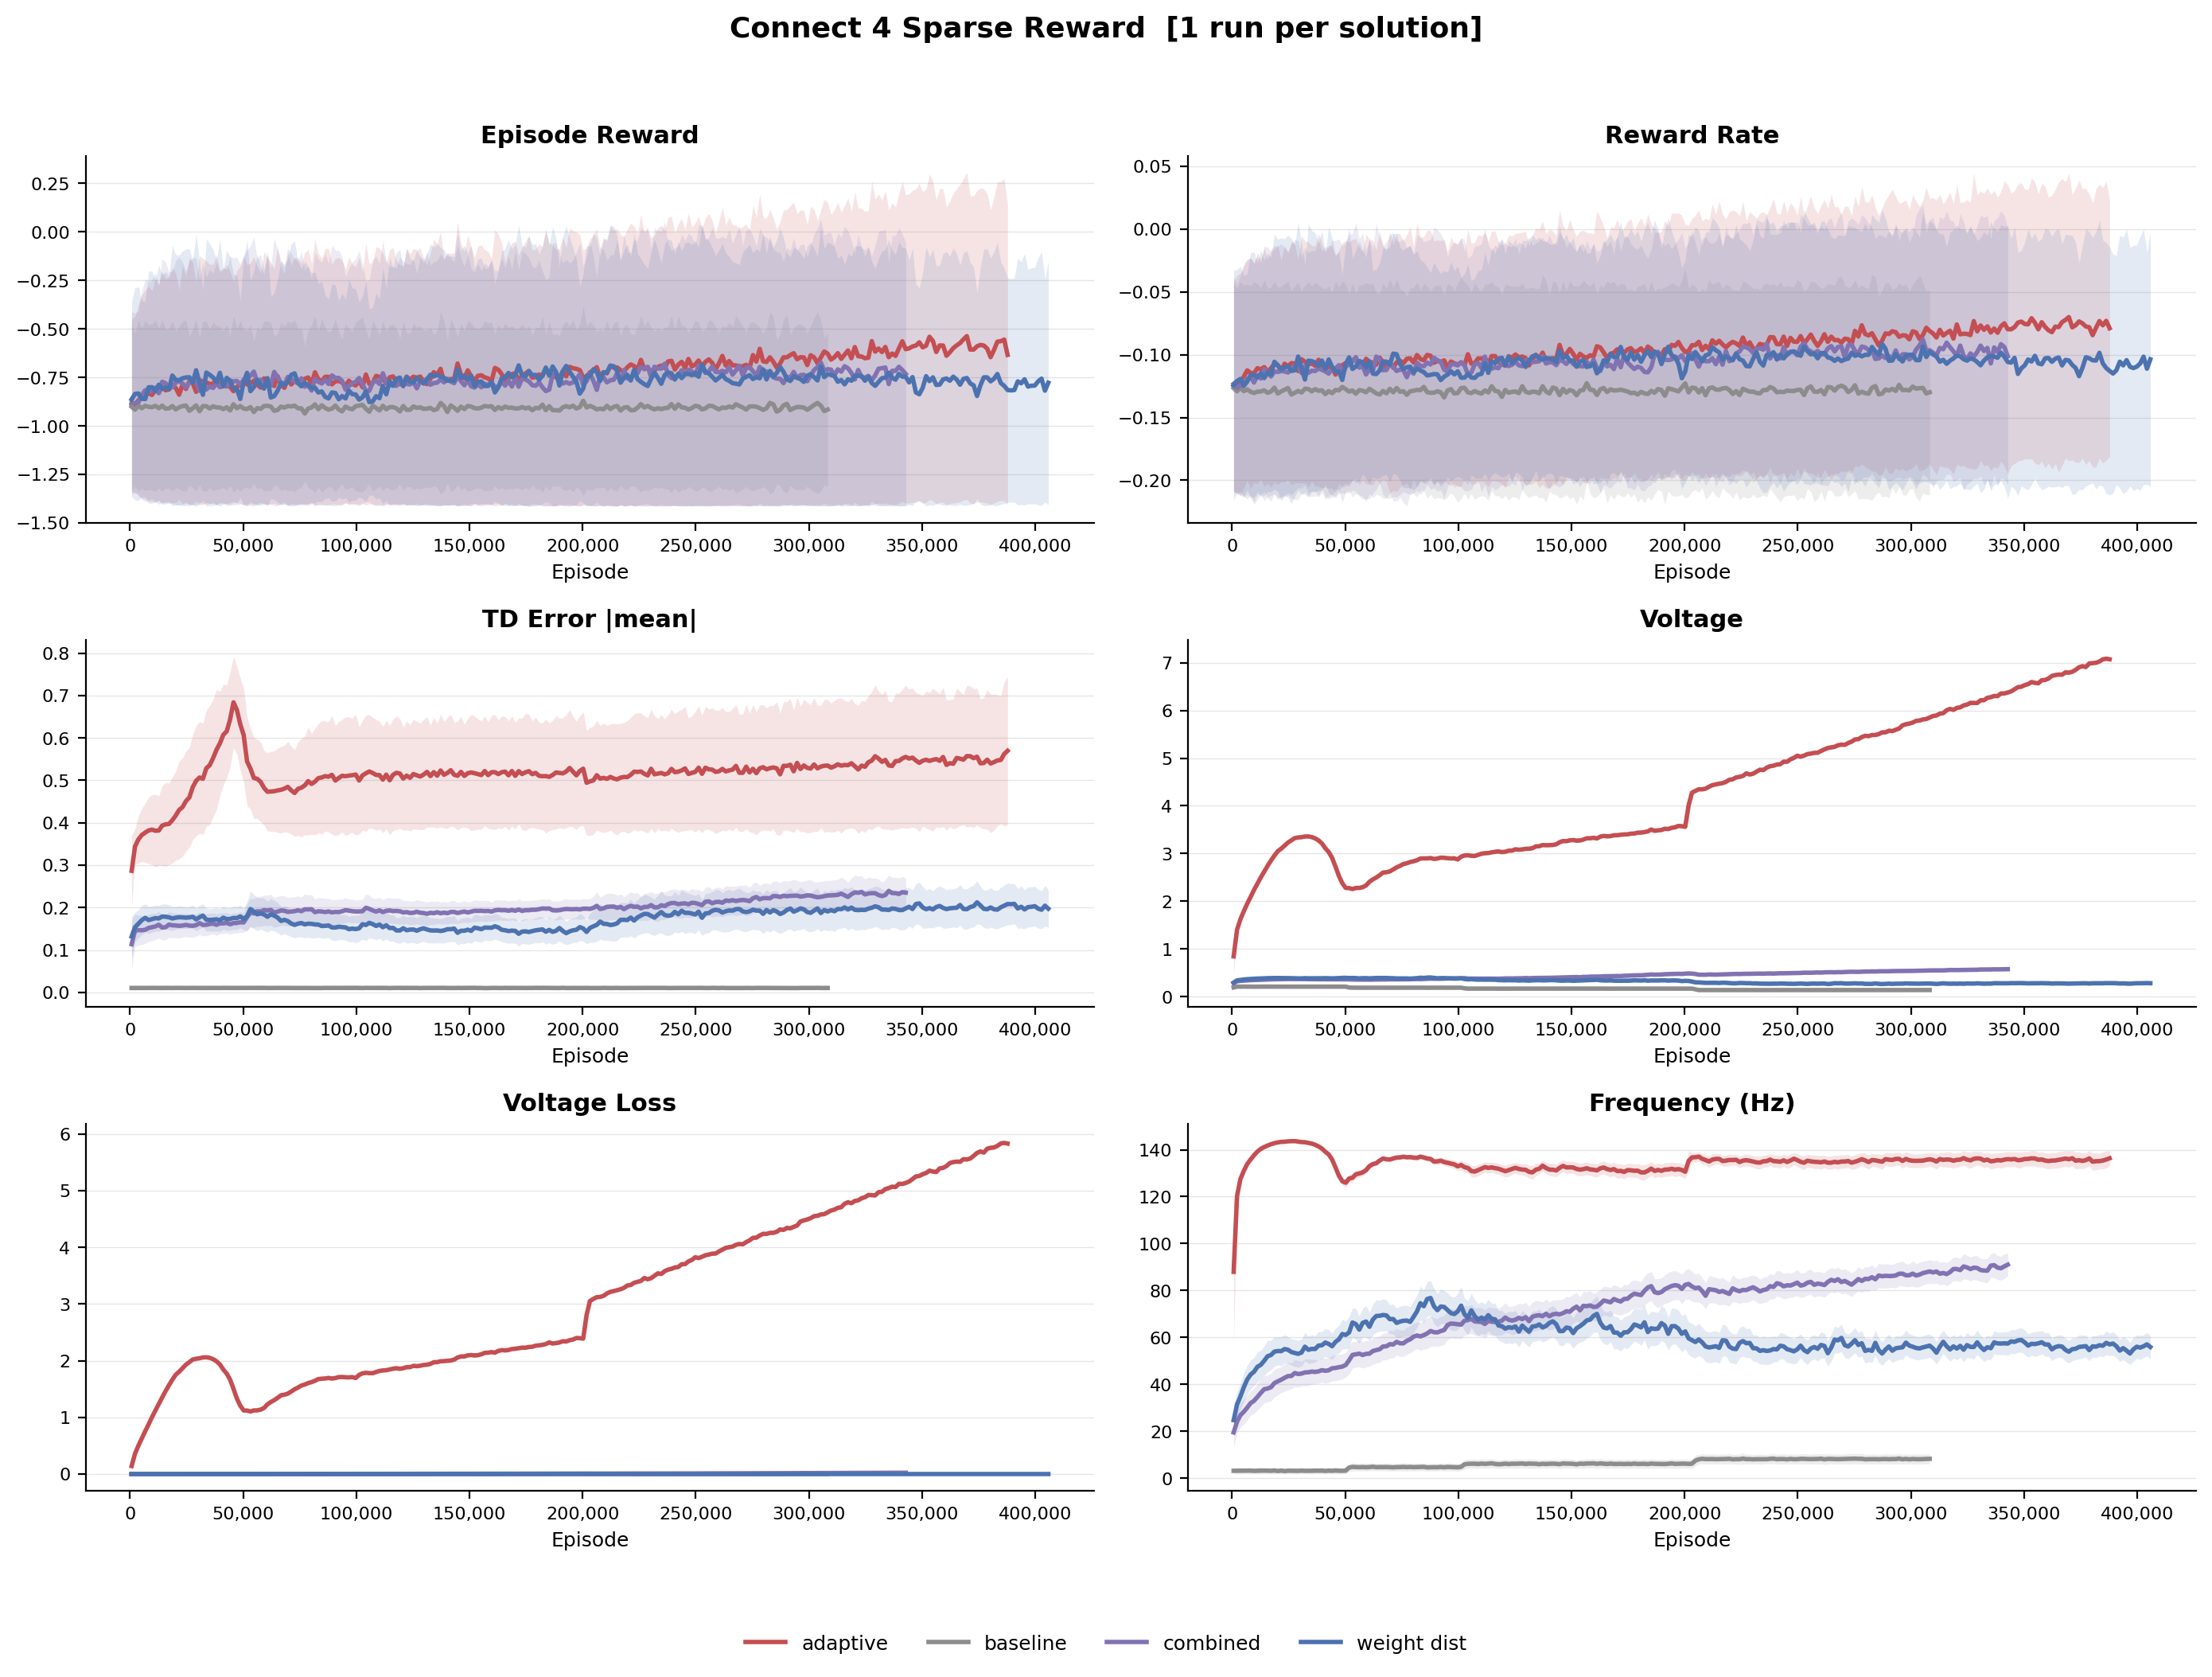
\includegraphics[width=1.0\textwidth]{images/comparison_misc_1_runs.png}
    \caption[Connect Four with sparse reward]{Training on Connect Four with a sparse terminal
    reward, comparing adaptive e-prop (red), \emph{weight dist} (blue), \emph{combined} (purple),
    and the \emph{baseline} (grey). One run per configuration; the six standard metrics are shown
    over roughly $400{,}000$ episodes. No configuration reaches a positive episode reward or reward
    rate. Adaptive e-prop shows a slight upward trend in both performance metrics, but with steadily
    growing voltage, voltage loss, and TD error, while the baseline remains essentially inert.}
    \label{fig:connect-four}
\end{figure}

None of the rules learns to play the task well, episode reward and reward rate remain negative
throughout training for every configuration. A consistent ordering nonetheless emerges in both
performance panels: adaptive e-prop sits highest and shows a slow but visible upward trend in episode
reward and reward rate, the distributed variants \emph{weight dist} and \emph{combined} follow close
behind and roughly flat, and the \emph{baseline} remains lowest and essentially flat.
The spiking-dynamics panels make clear that whatever progress adaptive e-prop makes comes at the cost
of increasingly pathological internal activity. Its membrane voltage and voltage loss do not stabilize
but climb steadily throughout training, reaching values far above any seen elsewhere in this chapter
(a voltage of around seven and a comparable voltage loss), and its mean absolute TD error sits at a
very high level, roughly an order of magnitude above the other rules. Its firing frequency saturates early in a high band around $140$~Hz. The \emph{baseline}, at the opposite extreme, is effectively
inert, its TD error stays near zero, its voltage and voltage loss remain flat and low, and its firing
rate is close to silence, the signature of a network that is not meaningfully learning a value
function or driving its neurons at all. The variants \emph{weight dist} and \emph{combined} occupy the middle
ground, with low and stable voltage and voltage loss and intermediate firing rates that drift upward
modestly, \emph{combined} rising to a higher frequency than \emph{weight dist}.

This is not a strong result, and we present it mainly to show that tasks of this kind, with a sparse
terminal reward and a long credit-assignment path, are hard for all of the learning rules considered:
none reaches a positive reward within the budget tested. What it does suggest is that adaptive e-prop
retains an advantage in learning the policy over the distributed variants even here, as it is the only
rule with a clear upward trend in episode reward and reward rate, albeit while its voltage, voltage
loss, and TD error grow steadily.

\section{Summary of the Experiments}
\label{sec:experiments-summary}

This section condenses the chapter into the messages a reader should retain.
The takeaways below are the substantive findings; the separate reading guide that follows explains
how confidently each should be held and addresses the recurring caveats.

\subsection*{Key takeaways}

\begin{itemize}
  \item \textbf{Metrics.} In the continuing, no-reset setup the operative objective is closer to the
  reward rate than to per-episode return; the two must be read together, as they can even move in
  opposite directions.
  \item \textbf{Objective horizon.} The episodic vs.\ continuing gap is set by $\gamma$, not
  $\lambda$: large at $\gamma=0.99$, nearly gone at $\gamma=0.5$. $\gamma$ fixes \emph{what} is
  optimized; $\lambda$ only sets the credit-assignment window.
  \item \textbf{Best rule on Snake.} \emph{symmetric} e-prop is the strongest single configuration,
  with the healthiest dynamics, but it collapses once the per-head field layers lengthen the causal
  path, because its feedback is tied to the output weights.
  \item \textbf{Best distributed optimizer.} Among the distributed variants, \emph{weight dist}
  optimizes best, in particular shared-postsynaptic-noise formulation.
  \item \textbf{The pseudo-derivative $\psi$ is essential.} Removing the heuristic surrogate factor
  $\psi^t_j$ (\emph{weight dist no heuristic}) collapses performance and lets the membrane voltage
  diverge (Section~\ref{sec:snake_comparison}); $\psi$ is not optional for these rules to work.
  \item \textbf{Adaptive and distributed are qualitatively different learners.} They differ less in
  final score than in \emph{how} they learn, in both spiking dynamics and the time-course of
  training. Concretely:
  \begin{itemize}
    \item \emph{Adaptive $\rightarrow$ pathological dynamics:} most prone to runaway voltage,
    voltage loss, and high firing rates, increasingly so as the causal path lengthens.
    \item \emph{Distributed $\rightarrow$ better value functions:} more stable, better-structured
    value estimates and well-regulated dynamics.
    \item \emph{Adaptive $\rightarrow$ policy edge:} on the two long-running examples (the extended
    five-layer network, Figures~\ref{fig:snake-extended-perstep}
    and~\ref{fig:snake-extended-perepisode}, and Connect Four, Section~\ref{sec:connect_four}) it is
    the only rule that keeps improving the policy, despite its noisier value estimates.
    \item \emph{Depth is a budget artifact:} at a fixed budget distributed e-prop looks more
    depth-robust, but with longer training adaptive starts slowly (feedback alignment) and then
    overtakes the distributed variants, which plateau early (Section~\ref{sec:snake_comparison}).
    \item \emph{Distributed tolerates model variations:} they could cope better with changes to the neuron
    model, e.g.\ the no-integration-during-refractory variant
    (Section~\ref{subsec:no_refractory_integration}).
  \end{itemize}
  \item \textbf{Combination adds little.} The hybrid \emph{combined} rule does not clearly
  outperform its parts, and is surprisingly the weakest on the deep per-episode run despite a strong
  showing in the one-layer comparison.
  
  \item \textbf{Update schedule.}Per-episode updates clearly help both rules on the deep (5-layer) network in Snake. On Pac-Man and Connect Four we did not run the per-episode/per-step comparison directly, though we informally observed that per-action updates tended to collapse on these tasks; we leave a systematic comparison for future work
  
  \item \textbf{regularization.} Voltage regularization works well because it is local; frequency
  regularization is harder; too much regularization strength degrades task performance.
  \item \textbf{Lambda robustness.} Neither rule is uniformly more $\lambda$-robust: distributed
  e-prop tolerates a wider $\lambda$ range on Pac-Man but shows two distinct failure modes at large
  $\lambda$ (runaway high activity vs.\ excessive silence), and the ordering is reversed on Snake.
  \item \textbf{Why deep nets fail (qualitative).} Deeper \emph{weight dist} networks develop flat,
  unstructured value estimates and near-deterministic policies, i.e.\ they lose exploration.
  \item \textbf{Hardest task: Connect Four (sparse reward).} Hard for every rule and solved by none;
  consistent with the policy-edge point above, adaptive e-prop shows the only positive learning
  trend.
  \item \textbf{The model assumptions are sound.} The \emph{baseline}, in which the recurrent
  weights are not trained, stays essentially flat in every experiment where it was tested, so the
  recurrent learning these rules perform is doing real work, the gains are not an artifact of the
  architecture or readout alone.
    \item \textbf{High firing rates are pervasive.} All learning rules across all
    tasks converge to firing rates of roughly 130 to 170~Hz, far above both the
    biological range and the $F^* = 10$~Hz regularization target. Our hypothesis is
    that the tasks studied require near-constant firing for reactive value and
    policy estimation, and that without a clear learning signal the dynamics tend
    to drift toward saturated activity.
\end{itemize}

\chapter{Conclusions}
\label{ch:conclusions}

\section{Summary of Contributions}
\label{sec:summary_contributions}

This thesis set out to study whether recurrent spiking neural networks can
learn effectively in fully online reinforcement learning settings using
learning rules that rely only on local computations and a globally
broadcast reward signal, and made two main contributions toward answering
this question.

The first contribution is the implementation of a continuously running reinforcement-learning agent
based on an excitatory-inhibitory recurrent spiking neural network, trained online with the e-prop
framework \citep{eprop2020}, without episodic resets, on a GPU-accelerated, event-based simulation
substrate \citep{Yavuz2016GeNN}. This online, single-agent, no-reset formulation is a strict setting
for reward-based e-prop, and we did not find an existing implementation run under the same
conditions to compare against directly. As part of this implementation we also integrated
TD($\lambda$) into the e-prop update, decoupling the discount factor $\gamma$ from the credit-trace
decay $\lambda$, a formulation used throughout the experiments in Chapter~\ref{ch:results}.

The second contribution is \emph{distributed e-prop}, a new family of learning rules that eliminates
the structured feedback weights used by standard e-prop to route loss information back to each
neuron. Building on the theoretical connection between perturbation-based learning and policy
gradient methods, every neuron is instead treated as an independent stochastic actor that perturbs
its own membrane dynamics and correlates this local exploration with a single, identical, globally
broadcast temporal-difference error. The key novel ingredient that makes this work is the heuristic
introduction of the pseudo-derivative $\psi^t_j$ as a gating factor on the local signal, although the
perturbation derivation does not by itself call for it, borrowing $\psi^t_j$ from e-prop concentrates
each neuron's update on the moments when its membrane is near the firing threshold, where its
perturbations actually influence spiking, and suppresses it otherwise. This heuristic gating turns
out to be essential, removing it collapses learning and lets the membrane
voltage diverge (Chapter~\ref{ch:results}). Several variants of the rule were derived,
differing in where the perturbation is injected (at the neuron or at the synapse) and in whether the
local perturbation signal is additionally routed through the recurrent connectivity, and these
variants were evaluated against standard e-prop with adaptive feedback on
three reinforcement learning tasks of varying complexity.

\clearpage
\section{Main Findings}
\label{sec:main_findings}

The experiments in Chapter~\ref{ch:results} support several
findings that, taken together, characterize when and how each family of
learning rules succeeds or fails.

\paragraph{In the continuing, no-reset setting the reward rate is the natural measure of performance,
and the small discount factor the spiking rules need for a stable critic limits the \emph{policy}
they can learn with respect to it.} Using PPO only as a reference optimizer to probe the objective, the ceiling
experiments (Section~\ref{sec:ppo_ceiling}) show on Snake $5\times5$ that with a large
$\gamma = 0.99$ the episodic and continuing formulations lead to markedly different policies, one
favouring episode return and the other the reward rate, each poor on the other, whereas a small
$\gamma = 0.5$ reaches a good policy under neither, settling into a compromise that is suboptimal on
both metrics. Crucially, this is a limit on the achievable policy, not on the network's ability to
learn. The spiking rules
operate in exactly this small-$\gamma$ regime and reach roughly the operating point the reference
optimizer attains there, so on this task they sit near the ceiling \emph{for that regime}, what holds
them back is the regime itself, not their credit assignment. Decoupling $\lambda$ from $\gamma$
(Section~\ref{sec:practical-lambda}) is the natural way to try to lift this, keeping a small $\gamma$
for critic stability while extending the credit horizon through $\lambda$, but it is self-limiting:
as the same experiment and the analysis in Section~\ref{sec:ppo_ceiling} show, once the
critic predicts the relevant rewards well the higher-order terms a larger $\lambda$ would contribute
vanish, so the longer credit assignment is effectively switched off precisely where the critic is
accurate, and $\lambda$ can extend the policy's effective horizon only where the critic cannot
predict those rewards.

\paragraph{Symmetric e-prop fails as causal path length grows, and this
motivates the alternatives studied in this thesis.} On Snake $5\times5$,
symmetric e-prop was the strongest individual configuration tested, but
its performance collapsed entirely once per-head field layers were
introduced between the recurrent core and the output heads
(Section~\ref{sec:symmetric-failure}). Because its feedback weights are
tied directly to the forward output weights, any neuron not directly
connected to an output head receives no feedback signal whatsoever once
the causal path length exceeds one. This is not a gradual degradation but
an outright failure mode, and it directly motivates both random/adaptive
e-prop, whose feedback is decoupled from the forward weights, and
distributed e-prop, which removes structured feedback altogether.

\paragraph{Distributed e-prop is competitive with, and sometimes faster than, adaptive e-prop, but with
a lower asymptotic ceiling in some settings.} Across the Snake and Pac-Man comparisons
(Sections~\ref{sec:snake_comparison} and~\ref{sec:pacman_comparison}),
several distributed e-prop variants reached usable policies as quickly or more quickly than adaptive
e-prop within the fixed training budget used throughout this thesis. Over longer horizons, however,
the ordering can reverse. On the extended five-layer Snake network (Section~\ref{subsec:snake-depth-comparison}),
the distributed variants converged within the first few thousand episodes and then plateaued, while
adaptive e-prop, after an extended period of near-zero reward consistent with the time feedback
alignment takes to take effect, continued improving past the distributed variants' plateau for the
remainder of the roughly $100{,}000$-episode run. The Connect Four results
(Section~\ref{sec:connect_four}) are consistent with the same ordering, adaptive e-prop ends up
highest and still slowly climbing while the distributed variants stay flat, although on that task the
runs differ in length, no rule reaches a usable policy, and adaptive's continued gain coincides with
steadily worsening spiking dynamics. Neither rule
should therefore be read as uniformly faster or uniformly better; their relative standing depends on
both the training budget and the task at hand.

\paragraph{Neither learning rule is uniformly more robust to the choice of
$\lambda$, and the two tasks studied gave opposite answers.} On Snake
$5\times5$ (Section~\ref{sec:snake_lambda_comparison}), adaptive e-prop
tolerated nearly the full range of $\lambda$ tested, failing only at the
most extreme value, while the distributed variant showed a narrower and
less monotonic band of values for which it learned promptly. On the
Pac-Man randomized layouts problem
(Section~\ref{sec:pacman_comparison}), the
distributed variant tolerated a wide range of $\lambda$, while adaptive
e-prop showed an inconsistent and often delayed learning onset across the
same sweep. This reversal is itself one of the more informative results
in this thesis, since it demonstrates directly that robustness to the
credit-assignment horizon is not an intrinsic property of either
algorithm, but depends on the task, and possibly on other interacting
factors such as architecture depth or reward sparsity that differ between
the two environments.

\paragraph{Distributed e-prop exhibits at least two distinct failure modes
under a poorly chosen $\lambda$, not one.} On the Pac-Man sweep, large
values of $\lambda$ destabilized the network's spiking dynamics, but not
always in the same direction, some values drove the network toward
runaway, pathologically high firing, while at least one drove it toward
the opposite extreme of excessive silence. Both are consistent with the
underlying credit trace losing useful information at long horizons, but
the fact that the same learning rule can fail in either direction, under
broadly similar conditions, suggests that the relationship between
$\lambda$ and network-level stability in this family of rules is more
intricate than a simple variance argument would predict.

\paragraph{The perturbation-based structure of distributed e-prop enables a
form of local reward shaping that standard e-prop could not support in
the same way.} The voltage-regularization experiment
(Section~\ref{sec:regularization-exploration}) found that a local,
perturbation-gated voltage reward could be used to keep membrane
potentials in a well-regulated range for distributed e-prop, while the
analogous regularization term applied within standard e-prop caused
membrane voltages to diverge instead of stabilizing it. The likely explanation
is that the perturbation trace naturally carries little signal when the
membrane is far from threshold, gating the regularization update away
from precisely the regime in which it would otherwise be poorly directed,
a self-suppression property that the standard e-prop update lacks.

\paragraph{Distributed e-prop is markedly more robust to a violated
modeling assumption in the neuron model than adaptive e-prop in at least one
observed setting.} When
membrane integration was disabled during the refractory period, a change
that invalidates an assumption in the analytical derivation of standard
e-prop's eligibility trace, adaptive e-prop failed to learn at all on the
Pac-Man randomized layouts problem, while the distributed variants
continued to learn successfully and maintained well-regulated spiking
dynamics (Section~\ref{subsec:no_refractory_integration}). This is consistent
with distributed e-prop's credit assignment being based on perturbation
correlations, which makes it comparatively insensitive to violations of the
specific assumptions that decomposition relies on.

\paragraph{The heuristic pseudo-derivative gating is essential to distributed e-prop, not an optional
refinement.} Although the perturbation-based derivation does not itself require it, gating each
neuron's local update by the pseudo-derivative $\psi^t_j$, so that credit accrues chiefly when the
membrane is near the firing threshold, proves necessary for the rule to learn at all. The ablation
that removes this factor (\emph{weight dist no heuristic}, Section~\ref{sec:snake_comparison}) does
not merely learn more slowly ,its performance collapses well below every other recurrent variant and
its membrane voltage diverges, growing without bound. This identifies the heuristic gating as a load-
bearing component of the rule, and suggests
that concentrating credit on the threshold-crossing regime, where a neuron's perturbations actually
affect its spiking, is what keeps the perturbation-based update both well-directed and dynamically
stable.

\paragraph{Distributed e-prop learns representations from which the value head regresses faster and more
cleanly than adaptive e-prop does, even though it carries no information about how it affects the
value function, which is one of the most surprising results of this work.} Across the qualitative
value-trace comparisons (Section~\ref{sec:value-traces}, Figure~\ref{fig:value_function_comparison}),
the distributed variants develop sharper, more anticipatory value estimates earlier in training than
adaptive e-prop, indicating that their recurrent representations are more readily linearly decodable
into an accurate value signal. This is counterintuitive given the two rules' information content:
adaptive e-prop routes an approximation of the loss gradient back through its feedback weights, so it
carries an approximate value gradient, an explicit signal of how each neuron should change to reduce
the value-prediction error, whereas distributed e-prop has no analogue at all, assigning credit only
from the correlation between local perturbations and a single broadcast scalar. On the value-function
regression task specifically, the gradient-aligned rule would therefore be expected to hold the
advantage, and yet the perturbation-based rule produces the more value-friendly representations. The
result suggests that shaping a representation that supports value estimation does not require an
explicit value gradient, and that the perturbation-based dynamics confer some advantage on
representation learning that the structured-feedback rule does not, an effect worth isolating in
future work.

\paragraph{The learning rules studied here are genuinely different objects, not minor variants of one
another, and distributed e-prop in particular performs surprisingly well given how much it gives up,
which makes it a promising target for further study.} Throughout the experiments the rules differed
not only in final performance but in how they learned, in their spiking dynamics, their sensitivity
to depth and to $\lambda$, their failure modes, and their robustness to violated modeling
assumptions, so they are better understood as distinct credit-assignment mechanisms that each
warrant study in their own right than as interchangeable choices. What stands out most is that
distributed e-prop remains competitive at all under the strictest constraints considered in this
thesis, it discards the structured feedback weights of standard e-prop entirely, assigns credit from
nothing more than the correlation between each neuron's own local perturbation and a single,
globally broadcast scalar TD error, and does so fully online and in constant memory. That a rule this
unconstrained can match or, in some settings, outpace adaptive e-prop, tolerate a violated neuron
model that defeats it, and support local reward shaping it cannot, is the most surprising outcome of
this work. It strongly suggests that distributed e-prop is worth studying further, both to map where
its advantages hold and to find the tasks and regimes that expose its limits.

\paragraph{High firing rates are a consistent operating regime, not a
pathology of any single rule.} Across all experiments, all learning rules, and
all three tasks, firing rates converge to a band of roughly 130--170~Hz,
far above both the biological range ($\approx$5--20~Hz) and the target rate
$F^* = 10$~Hz used in the firing-rate regularization. This holds regardless of
credit-assignment strategy, network depth, or task. The firing-rate
regularization term imported from standard e-prop proves insufficient to keep
rates near the target. Our hypothesis is that the some of the tasks studied here 
(Snake, Pac-Man) modeled as they are in this work, 
are highly reactive, requiring the network to maintain near-constant 
firing to produce value and policy estimates at every
step, which pushes the dynamics toward dense activity. Additionally, when the
learning signal is weak or absent, the dynamics tend to drift toward
saturation, as the mechanisms that would otherwise
reinforce sparse, informative firing patterns lack the signal to do so.
Whether stronger rate-control mechanisms or tasks with different temporal
structure would allow the network to settle into a sparser regime remains an
open question.

\paragraph{A single, globally broadcast scalar signal is enough to train recurrent spiking networks
effectively online, though with qualifications.} The question of whether credit assignment from
nothing more than local computation and one identical, globally broadcast reward-related signal can
drive effective learning, recurring throughout this thesis, is answered here in the affirmative for
the tasks studied: the distributed e-prop variants learn non-trivial behavior on Snake and Pac-Man,
including the anticipatory, partially observable navigation the latter requires, and do so fully
online, in constant memory, and within training budgets comparable to, and at times shorter than,
those of the gradient-aligned adaptive rule. The qualifications are equally part of the finding. The
extended-training comparison shows the distributed variants plateauing below adaptive e-prop's
eventual ceiling (Section~\ref{subsec:snake-depth-comparison}), the usable range of $\lambda$ is
task-dependent and can destabilize the dynamics when poorly chosen, and the hardest, maximally
sparse task, Connect Four, was not solved by any rule (Section~\ref{sec:connect_four}). The
broadcast signal is therefore sufficient to learn fairly complex policies efficiently, but not
without limits on asymptotic performance and on the difficulty of task it can currently reach.

\section{Limitations}
\label{sec:limitations}

Several limitations should be kept in mind when interpreting the results
of this thesis.

\paragraph{Most comparisons rely on a small number of runs, and several of
the depth and $\lambda$ sweeps reported in
Chapter~\ref{ch:results} are single runs per configuration.} Where
this is the case, it has been noted explicitly alongside the relevant
results, but it means that some of the more striking individual
observations, such as the specific failure of $\lambda = 0.4$ for the
\texttt{combined} variant on Snake, or the specific failure mode taken by
$\lambda = 0.9$ for \texttt{weight\_dist\_prop} on Pac-Man, cannot be
distinguished from idiosyncrasies of that particular run without repeated
seeds. The five-run comparisons presented for the primary Snake and
Pac-Man evaluations are more robust in this respect, but even there, the
hyperparameters were not tuned exhaustively for any single learning rule,
and a configuration that favors one rule may be poorly matched to
another, as noted repeatedly throughout Chapter~\ref{ch:results}.

\paragraph{No direct comparison was made against Truncated Backpropagation Through
Time as upper-bound baseline for task
performance.} The motivation for this thesis is squarely the online,
constant-memory setting in which this method is not applicable
in its unmodified form, but this also means that the absolute
performance ceiling achievable on these tasks is not known for the arquitectures
tested in this thesis. If the requirements were relaxed, 
we could test how these architectures would work using TBPTT and test it against 
the presented rules.

\paragraph{Several proposed extensions of distributed e-prop did not work
reliably enough to be included in the main comparisons.} The per-synapse
exploration-variance update (Section~\ref{subsec:exploration_variance}) was
found to add complexity without a clear benefit over the simpler
neuron-level update, and was therefore kept fixed in the main
experiments. The propagation of local regularization rewards through the
structured-routing machinery (Section~\ref{subsec:regularization}) showed
promising preliminary results but was not investigated systematically.

\section{Future Work}
\label{sec:future_work}

The limitations and open questions identified throughout this thesis
suggest several directions for future work, ranging from immediate
methodological extensions to more open-ended questions about how local,
perturbation-based learning rules might be developed further.

\paragraph{Systematic characterization of the discount $\gamma$.}
Throughout this work the discount was fixed to $\gamma = 0.5$ on the basis of
initial empirical exploration. This was
sufficient to obtain stable learning, but it leaves the role of $\gamma$
largely uncharted in our setting. The decoupling introduced in
Section~\ref{sec:decoupled-lambda-rule} now makes such a study well-posed, since
$\gamma$ is confined to the critic and no longer constrains the actor's credit
horizon, its effect is cleanly isolated to value estimation, and a dedicated
$\gamma$-sweep can be interpreted without confounding it with the
action-credit-assignment range. A natural next step is therefore to map, for
each learning rule, how critic learnability degrades as $\gamma$ grows,
identifying the point at which the compounding of small per-step value errors
across bootstrapping destabilizes the target $\delta_t = R_{t+1} + \gamma V_{t+1} -
V_t$ and the value head ceases to converge. Because the learning rules differ
in how they route the global feedback signal, their critics may tolerate
different maximum discounts; characterizing this per-rule threshold would
clarify whether the aggressive discount required here is a fundamental
constraint of the continuing, no-reset setting with a noisy spike-based critic,
or an artifact specific to certain rules. The interaction with an optional
critic-specific $\lambda_V$ and with the absence of episodic resets would be
worth examining in the same sweep.

\paragraph{Combining structured feedback and perturbation-based credit
assignment more deliberately.} Distributed e-prop was originally
conceived as a way of correcting the bias introduced by the approximate
feedback weights of standard e-prop, by supplementing the
structured learning signal with a perturbation-based estimate. In
practice, the \texttt{combined} variant explored in
Chapter~\ref{ch:results}, which simply sums the synaptic
perturbation update with the adaptively routed feedback update, behaved
similarly to the perturbation-only variants and did not show a clearly
synergistic improvement over either rule in isolation. This is somewhat
surprising given the flexibility of the underlying framework, and it
seems unlikely that no combination of the two signals can outperform
each individually. More structured ways of combining them remain
unexplored, the two signals could be weighted dynamically, 
for instance based on the agreement between the two estimates, 
in a manner similar to the heuristic agreement 
term already introduced for the perturbation and
backrouted traces in Section~\ref{subsec:structured_routing}; the feedback
signal could be used primarily as a variance-reduction term early in
training, when the perturbation-based estimate is least reliable, and
phased out as the feedback weights converge; or the two updates could be
applied to disjoint subsets of weights. 
Identifying a combination strategy that reliably outperforms
both constituent rules would be a natural next step.

\paragraph{Ablating the role of learned output weights.} As discussed in
Section~\ref{subsec:neuron_as_actor}, the output weights receive an exact
gradient at every step, unlike the perturbation-based estimates that drive the
recurrent layer, and the quality of the readout they learn largely determines
how informative the broadcast error $`\delta_t`$ is for the hidden neurons.
This suggests that much of the early learning may be driven by the readout
adapting to the recurrent layer's initial dynamics. A dedicated ablation
study (freezing the output weights at random initialization, or delaying
their learning for a fixed number of steps) would help disentangle how much
of the learning is attributable to the recurrent rule versus to the
adaptation of the readout that supplies its credit signal.

\paragraph{Alternative gating functions for the pseudo-derivative modulation.}
The pseudo-derivative $`\psi_j^t`$ that gates the perturbation-based update
is a specific choice, not a theoretical necessity, as noted in
Section~\ref{subsec:lif_update_rule}, one could replace
it with alternative gating mechanisms, such as smoother functions of the
membrane potential, and still obtain valid variants of the update rule. The
ablation in Chapter~\ref{ch:results} showed that removing the gating
altogether collapses learning, but this does not establish that the
particular form of $`\psi_j^t`$ borrowed from e-prop is optimal. A
systematic study of alternative gating functions (for instance smooth
sigmoid-like thresholds with tunable width, or functions that depend on
the recent spiking history of the neuron) could reveal whether the current gating is merely
sufficient or close to best among a broader family, and whether the
threshold-crossing regime it concentrates credit on is the most informative
regime for perturbation-based updates in general.

\paragraph{Alternative routing weights for the distributed routing pathway.}
The routed variants of distributed e-prop reuse the recurrent weights
$`W^{\mathrm{rec}}`$ themselves to propagate each neuron's local signal through
the network (Section~\ref{sec:feedback_connectivity}), which makes the routing
symmetric by construction, tied directly to the forward connectivity. This is
only one of the choices available, and it mirrors symmetric e-prop. The same
decoupling explored for standard e-prop's feedback matrices could be applied
here as the distributed routing could instead use a fixed random projection or an
adaptively learned matrix, separate from $`W^{\mathrm{rec}}`$, yielding random
and adaptive analogues of the routed distributed variants. Studying these would
clarify whether the benefits of routing the local signal stem specifically from
its alignment with the forward recurrent weights, or whether any structured
projection of the local signals across the population suffices, paralleling the
question of how much symmetric e-prop's performance depends on weight alignment
versus merely having a structured feedback path at all.

\paragraph{Exploring a gated per-neuron exploration-variance update.} The
per-neuron exploration variance $`\sigma_j`$ was held fixed throughout the
main experiments, and the adaptive update proposed in
Section~\ref{subsec:exploration_variance} did not yield a clear benefit over
a fixed value. One possible reason is that the variance update, as
formulated, accumulates credit from perturbations regardless of whether the
neuron's membrane was near threshold at the time, even though it is
precisely in that near-threshold regime that the perturbation actually
influences spiking. The pseudo-derivative gating $`\psi_j^t`$ was shown to
be essential for the weight update for exactly this reason, but the
variance update has no analogous mechanism. A natural direction is to
apply a similar gating factor to the $`\sigma_j`$ update, so that the
variance is adapted predominantly from perturbation correlations at
moments when the neuron's perturbations were behaviorally relevant. This
could reduce the noise in the variance estimate itself and potentially make
the adaptive $`\sigma_j`$ update viable where the ungated version was not.

\paragraph{Richer and state-dependent exploration.} The exploration variance
$\sigma_j$ used throughout this thesis is either a fixed hyperparameter
or, at best, a per-neuron scalar updated by its own local policy gradient
(Section~\ref{subsec:exploration_variance}), with no dependence on the
network's current state. A natural extension is to make $\sigma_j$ a
function of context, for instance increasing exploration in states where
the value estimate is uncertain or rapidly changing, and decreasing it
once a stable policy has been found for a given region of the state
space. This connects directly to ideas from meta-learning, since a
state-dependent exploration policy is itself a learned controller that
shapes how the underlying weights are updated, an instance of the network
modulating its own learning; we return to
this connection below. A second, largely orthogonal direction concerns
the structure of the injected noise itself. The perturbation variants
studied in this thesis inject either fully independent noise per neuron
or per synapse, or a single shared sample per postsynaptic neuron scaled
individually per synapse (Section~\ref{subsec:synaptic_perturbation}).
An interesting intermediate possibility, not explored here, is to draw
the perturbation noise from a small shared latent space, with a low-
dimensional noise vector sampled once per timestep and projected onto
each neuron or synapse through a fixed or learned projection. This would
deliberately correlate the exploration noise across the population,
in a manner reminiscent of how evolution strategies can benefit from
structured perturbations, and could offer
a different point in the bias-variance tradeoff than the perturbation
variants compared in Chapter~\ref{ch:results}.

\paragraph{A broader family of local reward signals.} The voltage- and
firing-rate-regularization rewards introduced in
Section~\ref{subsec:regularization} demonstrated that distributed e-prop can
incorporate purely local evaluative signals, compatible with its
perturbation-based update, in a way that standard e-prop could not
support as effectively. Voltage and firing rate are only two examples of
quantities a neuron could evaluate about itself; other candidates might
include the temporal sparsity or burstiness of a neuron's own spike
train, the correlation of a neuron's activity with that of its immediate
neighbors, or measures of how informative a neuron's recent activity has
been for the network's eventual output. More broadly, this raises the
question of what other local objectives admit a similarly natural
perturbation-based update, and whether a network exposed to several such
local rewards simultaneously, alongside the global task reward, would
develop qualitatively different internal representations than one trained
on task reward alone.

\paragraph{Structural plasticity and online rewiring.} Throughout this thesis the
network's synaptic topology was fixed at initialization, the toroidal Gaussian
connectivity, the excitatory-inhibitory partitioning, and the per-head field
layers were all static for the duration of training. Only the synaptic weights
were adapted. Yet in biological circuits, learning is not confined to changing
existing connection strengths; structural plasticity, including synaptic
formation and elimination, rewires the graph itself on a slow timescale, and
this process is thought to play a role in stabilizing dynamics and expanding
the functional representations available to the agent. An analogous mechanism
could be valuable in the setting studied here, particularly given the finding
that all learning rules converge to a high-firing regime with poorly
regulated membrane voltages (Section~\ref{sec:main_findings}).

\paragraph{Learning signals produced by a self-trained mechanism.} Throughout this thesis, the learning
signal each neuron receives is either a structured but fixed
approximation to the gradient, routed through feedback weights that are
random, symmetric, or themselves adaptively learned
(Section~\ref{subsec:eprop-variants}), or a single scalar TD error, identical
for every neuron, in the case of distributed e-prop.\
\citep{OneShotEprop} explore a related but distinct idea: a separate
network is trained to produce the per-neuron learning signal $L^t_j$
itself, taking on a role loosely analogous to dopaminergic areas of the
brain that gate plasticity elsewhere.

One possibility is a population of additional, self-trained neurons that
act as a kind of student network, learning online, alongside the main
network, to predict or shape the contribution each neuron should make to
the eventual outcome. A second, less architecturally
involved possibility is to give each neuron a supplementary learned
signal, produced by an additional set of
weights. A third possibility, echoing
the shared-latent-space idea discussed above for exploration noise, is to
project a small, shared, learned latent vector onto each neuron at every
timestep, so that neurons receive a population-level signal that is
richer than a single scalar but still far more constrained than a fully
structured, per-neuron feedback projection.

A point worth stressing for all three options is that, for them to remain
consistent with the rest of this thesis, whatever additional mechanism
produces these signals must itself be trained online, using the same
continuous stream of experience and the same constant-memory,
forward-in-time updates as the rest of the network. The appeal of distributed
e-prop is precisely that every component of its update is local and
online; a supplementary signal-generating mechanism that itself depended
on offline meta-training, or on machinery incompatible with the
online setting motivating this thesis, would reintroduce exactly the
kind of constraint the rest of this work tries to avoid. Whether a
self-trained signal of this kind, learned under the same online
constraints as everything else, can meaningfully enrich the credit
assignment available to each neuron without compromising locality is an
open question this thesis leaves for future investigation.

\paragraph{A more systematic exploration of architecture size and depth.}
The depth comparison in Section~\ref{subsec:snake-depth-comparison} varied the
number of layers for two specific learning rules on a single task, and
found that the two rules respond differently to depth within a fixed
training budget. This leaves open how either rule behaves as other
architectural dimensions are varied, such as the width of each
excitatory-inhibitory population, the fan-in of the toroidal Gaussian
connectivity, or the presence and size of the per-head field layers
independently of depth. A more systematic sweep across these dimensions,
ideally with the repeated seeds discussed above, would help separate
effects that are specific to causal path length from effects that are
more generally about network scale or capacity.

\paragraph{Tasks demanding longer-term memory.} The three environments
studied in this thesis were chosen to probe sparse-reward credit
assignment, working memory under partial observability, and behavioral
adaptation, but none of them require the agent to retain information over
very long horizons relative to the timescales of the underlying neuron
and adaptation dynamics. Tasks that demand longer-term memory, for
instance environments where relevant information must be retained for
hundreds or thousands of timesteps before it becomes useful, would test
the limits of the adaptive threshold mechanism's slow timescale 
and of the action-credit-assignment
horizon controlled by $\lambda$ considerably more severely than the tasks
studied here. Such tasks would also raise practical questions about how
training itself should be adapted, since a longer required memory horizon
may demand a correspondingly longer $\lambda$, which Chapter~\ref{ch:results}
showed can itself destabilize the algorithms spiking dynamics;
resolving this tension may require some of the other directions
discussed above, such as a state-dependent or self-modulated $\lambda$.

\paragraph{Repeated-seed evaluation of the depth and $\lambda$ sweeps.} The
single-run nature of several of the comparisons in this thesis, noted in
Section~\ref{sec:limitations}, means that converting the more striking
qualitative observations, such as the divergent failure modes of
distributed e-prop at large $\lambda$ on Pac-Man, into statistically
grounded claims would require repeating these sweeps across multiple
seeds.

\paragraph{A systematic study of the relationship between $\lambda$ and
network-level stability in distributed e-prop.} The observation that
large $\lambda$ can drive the network toward either runaway firing or
excessive silence, depending on the specific value and possibly the
random seed, is currently unexplained. Understanding what determines
which failure mode a given configuration falls into would clarify
whether this is a fundamental property of the perturbation-based update
or an artifact of the specific architecture and task studied here.

\paragraph{Deployment on neuromorphic hardware.} The implementation
developed in this thesis was deliberately constrained to be expressible
entirely in terms of local, per-synapse updates and event-driven
computation (Section~\ref{sec:implementation}), with the explicit
goal of acting as a faithful prototype for spike-driven accelerators such
as Loihi \citep{Davies2018Loihi} or SpiNNaker \citep{Painkras2013SpiNNaker}.
Carrying out this deployment directly would be a natural next step, and would allow
the energy-efficiency motivations discussed in Chapter~\ref{ch:introduction} to
be evaluated empirically.


\clearpage
\addcontentsline{toc}{chapter}{Bibliography}
\bibliography{references}

\end{document}